\documentclass[a4paper,11pt,twoside]{report}
%\documentclass[a4paper,11pt,twoside]{book}
\setcounter{errorcontextlines}{999}

% line spacing
\usepackage{setspace}
\onehalfspacing

%%%pre-amble%%%%%%%%
\usepackage{graphicx}
\usepackage{siunitx} % for degree symbols 90\si{\degree}C
\usepackage{hyperref} %this makes everything hyper-refed
\usepackage{parskip} % spaces between paragraphs instead of indents
\usepackage[font={small},labelfont={bf},margin=10pt]{caption} % make figure captions small and italic
%\usepackage{subfigure}
\usepackage{textgreek}
\usepackage{enumitem}
\usepackage{booktabs}
\usepackage{verbatim}
\usepackage{longtable}
\usepackage{multirow}
%\usepackage{color}
\usepackage{grffile}
\usepackage{amsmath, amsthm, amssymb}
\usepackage{lscape}
\usepackage[table,xcdraw]{xcolor}
\usepackage{setspace}
\usepackage{subfig}
\usepackage{makecell}
\renewcommand\theadalign{cb}
\renewcommand\theadfont{\bfseries}
\renewcommand\theadgape{\Gape[4pt]}
\renewcommand\cellgape{\Gape[4pt]}
\usepackage{multirow}
\usepackage{longtable}
\usepackage{flexisym} % for prime symbols \textprime
\usepackage{anyfontsize}
\usepackage{emptypage} % all cleardoublepage are without page numbers

\usepackage[round]{natbib}
\usepackage{pdfpages} % for adding pdfs in to the appendices
\usepackage{pdflscape} % for landscape pages
\usepackage{sidecap} % for side captions
\usepackage{gensymb} % for the degree symbol
\usepackage{titlesec, blindtext, color}
\definecolor{gray75}{gray}{0.75}
\newcommand{\hsp}{\hspace{1pt}}
\usepackage[a4paper,left=3.81cm,right=2cm,top=2cm,bottom=2.5cm,footskip=30pt]{geometry}

\titleformat{\chapter}[hang]{\Huge\bfseries}{\thechapter\hsp\textcolor{gray75}{|}\hsp}{0pt}{\LARGE\bfseries}
\titlespacing{\chapter}{0pt}{0pt}{1cm}

\usepackage[T1]{fontenc}
\usepackage[toc,page]{appendix}

\usepackage{fancyhdr} % for headings
\pagestyle{plain}

%\fancyhead[LO,RE]{}
%\fancyhead[RO,LE]{}
%\fancyhead[LE]{\textsl{\leftmark}}
%\fancyhead[RO]{\textsl{\rightmark}}

%\fancyhead[LE]{\textsl{\rightmark}}
%\fancyhead[RE]{\textsl{\leftmark}}
%\fancyfoot[C]{\thepage}
%\lhead{} 
%\fancyfoot[C]{\thepage}
%\addtolength{\headwidth}{\marginparsep}
%\addtolength{\headwidth}{\marginparwidth}
%\renewcommand{\chaptermark}[1]{\markboth{#1}{}}
%\renewcommand{\sectionmark}[1]{\markright{\thesection\ #1}}
%\fancyhf{}
%\fancyhead[LE,RO]{\textbf{\thepage}}
%\fancyhead[LO]{\textbf{\rightmark}}
%\fancyhead[RE]{\textbf{\leftmark}}



\usepackage{amsmath} % for equations
\setlength{\headheight}{12pt}
\graphicspath{{/Users/Jack/google_drive/Work/PhD_Year_4/Thesis/Figures}} %this is the path to all your figures


%%%%%%%%%%%%%%%%%%%%%%%%%%%%%%%%%%%%%%%%%%%%%%%5
\begin{document}

% FRONT MATTER

\begin{titlepage}%%%%%%%%%%%%%%%%%%%%%%%%%%%%%%
\newcommand{\HRule}{\rule{\linewidth}{0.5mm}}

\center 

%logo

\includegraphics[width=7cm]{Figures/misc/ucllogo.jpg}\\[1cm]
%headings
\textsc{\LARGE University College London}\\[2cm] % Name of your university/college
%title
\HRule \\[1cm]
%CHANGE TITLE?
{ \huge \bfseries RNA dysregulation in models of frontotemporal dementia and amyotrophic lateral sclerosis}\\[0.4cm] 
\HRule \\[2cm]


\textsc{\Large Doctoral Thesis}\\[1.5cm] % Minor heading such as course title


%Author
%\begin{minipage}[t]{0.8\textwidth}
%\begin{flushleft} \large
%\raggedright
\emph{Author:}\\
Jack \textsc{Humphrey}\\[1cm] % Author's Name
%\end{flushleft}
%\end{minipage}

%\begin{minipage}[t]{0.8\textwidth}
%\begin{flushright} \large
%\raggedleft
\emph{Supervisors:} \\
Prof. Adrian \textsc{Isaacs}\\ 
Dr Vincent \textsc{Plagnol}\\ 
Dr Pietro \textsc{Fratta}\\[1cm]


\textsc{\Large UCL Institute of Neurology}\\[0.5cm] % Major heading such as course name
\textsc{\Large UCL Genetics Institute}\\[2cm] % Major heading such as course name


%\end{flushright}
%\end{minipage}\\[3cm]

%date
%{\large \today}\\[3cm] 

\vfill % Fill the rest of the page with whitespace

\end{titlepage}%%%%%%%%%%%%%%%%%%%%%%%%%%%%%%%%%%%
\cleardoublepage
%\clearpage

%\phantomsection


I confirm that the work presented in this thesis is my own.  Where information has been derived from other sources, I confirm that this has been indicated in the thesis.

Jack \textsc{Humphrey}
\vfill




\cleardoublepage

%\phantomsection
%\begin{abstract}
\section*{Abstract}
%% update! 300 words max!

Amyotrophic lateral sclerosis (ALS) and frontotemporal dementia (FTD) are two rare but devastating neurodegenerative diseases that share pathological features and genetic factors. A central problem in  both diseases is understanding the role of RNA-binding proteins, exemplified by transactive response DNA-binding protein 43kDa (TDP-43) and fused in sarcoma (FUS). These proteins play a vital role in RNA regulation in all cells but in diseased neurons they alter their function to form potentially pathogenic aggregates. These can be linked to genetic mutations in some rare cases, although most cases of ALS/FTD have no known genetic cause. My work uses the revolutionary technology of RNA sequencing to understand changes in RNA expression, splicing and transport in different cellular and animal models of sporadic and genetic disease.\\
I present a meta-analysis of published RNA sequencing experiments which deplete TDP-43 or FUS as a crude model of sporadic disease. Using these datasets, I assess the evidence for cryptic splicing, an unusual RNA phenotype caused by a loss of mRNA splicing fidelity. I demonstrate that repression of cryptic splicing is a specific function of TDP-43 and not FUS. My analysis predicts that cryptic splicing leads to expression changes due to disrupted mRNA stability and may therefore be a cause of neurodegeneration in ALS and FTD.\\ 
I then describe work on a new mouse model of FUS-mediated ALS. I observe that gene expression changes are seen only in the spinal cord and not in the cortex. These expression changes are progressive, occurring late into the lifespan of the mice and are accompanied by motor neuron loss. The altered mRNAs are enriched in mitochondrial and ribosomal genes, which warrant further investigation into the mutant protein's role in translation and transport of its target mRNAs. 
Lastly, I map out the remaining projects for the rest of my PhD. My goal is to transfer the insight gained from the model work into establishing mechanisms of disease course and aetiology in the analysis of human patient data. 






%\end{abstract}
%\clearpage

\cleardoublepage

\section*{Impact Statement}

% intro
% aims of thesis
% how these insights are useful to the field
This thesis comprises four studies on TDP-43 and FUS, two RNA-binding proteins linked to the devastating neurodegenerative diseases Amyotrophic Lateral Sclerosis and Frontotemporal Dementia.
I analysed RNA sequencing data to develop insights in to the regulation of RNA by these two proteins in both normal physiology role and in models of disease.
This work has uncovered new roles for TDP-43 and FUS in specific types of RNA regulation.
Additionally, I have discovered new mechanisms to explain how disease-associated mutations in the two proteins affect these roles.
Conclusions from my work are broadly applicable to the RNA biology field as a whole as well as efforts to understand and treat these diseases.
%Following the Ice Bucket Challenge of 2014, there has been increasing public awareness of ALS and a large amount of money has been raised to research basic science. 
Insights into RNA-binding proteins and RNA regulation from this work can be transferred to many non-neurological diseases where RNA regulation plays a role, including muscular diseases, certain subtypes of cancer and retinal diseases \citep{Scotti2015}. 
Several of my chapters focus on developing new methods or adapting existing methods to analyse RNA splicing, a key mechanism of RNA regulation.
RNA-sequencing is becoming a standard experiment across all fields of biology and the use of sequencing data in analysis of RNA splicing is an area of extreme interest and method development. 

% impacts arising from this thesis:
Three peer-reviewed papers have been published from this thesis.
As of November 2018, "Quantitative analysis of cryptic splicing associated with TDP-43 depletion" \citep{Humphrey2017} has been cited 11 times, "Humanized mutant FUS drives progressive motor neuron degeneration without aggregation in FUS Delta14 knockin mice" \citep{Devoy2017} has been cited 11 times and "Mice with endogenous TDP-43 mutations exhibit gain of splicing function and characteristics of amyotrophic lateral sclerosis" \citep{Fratta2018} has been cited 7 times and was the subject of a "News and Views" article in The EMBO Journal \citep{Rouaux2018}.
These outcomes illustrate the importance of this work to the ALS/FTD and RNA biology fields.

Three new mouse models of ALS/FTD have been generated for projects carried out in this thesis: the FUS $\Delta$14 mouse, the TDP-43 RRM2mut mouse, and the TDP-43 LCDmut mouse. 
All three mice are available for labs around the world to use in further experiments.
RNA-seq data created from these mice have been made publicly available and can be downloaded from the Sequence Read Archive (\url{https://www.ncbi.nlm.nih.gov/sra}).
Several of my chapters rely on the re-analysis of published RNA sequencing data. 
I am pleased to see that sequencing data analysed in this thesis (chapter 5) has been re-used in a follow-up paper \citep{Sivakumar2018}.

I have tried to make all software written during this thesis publicly available where possible.
This is all available to download on the GitHub platform. 
 This includes the RNA-seq analysis pipeline used in all chapters\footnotemark , software developed to find and classify cryptic splicing (chapter 3)\footnotemark, and software written to classify splicing events found in the TDP-43 LCDmut and RRM2mut mice (chapter 5)\footnotemark.


\footnotetext[1]{\url{https://github.com/plagnollab/RNASeq_pipeline}}
\footnotetext[2]{\url{https://github.com/jackhump/CryptEx} }
\footnotetext[3]{\url{https://github.com/jackhump/Two_TDP-43_Mutant_Mice}}

\cleardoublepage

%\pagenumbering{roman}
\tableofcontents %prints table of contents
\listoffigures %prints list of figures	
\listoftables %prints list of tables

\section*{\LARGE{List of abbreviations}}
\begin{table}[h!]
	\begin{tabular}{ll}
		ALS & Amyotrophic lateral sclerosis \\
		CLIP & UV crosslinking and immunoprecipitation \\
		eCLIP & Enhanced UV crosslinking and immunoprecipitation \\
		ES cell & Embryonic stem cell \\
		ENU & N-ethyl-N-nitrosourea \\
		FDR & False discovery rate \\
		FTD	& Frontotemporal dementia \\
		FUS & RNA-binding protein Fused in Sarcoma \\
		GO & Gene ontology \\
		hnRNP &	Heterogeneous nuclear ribonucleoprotein\\
		iCLIP & Individual nucleotide resolution UV crosslinking and immunoprecipitation \\
		KO & Knockout \\
		LCD & Low complexity domain \\
		LCDmut & TDP-43 Low complexity domain mutation\\
		LINE & Long interspersed nuclear element \\
		MUT & Mutant \\ 
		NLS & Nuclear localisation signal \\
		NMD & Nonsense-mediated decay \\
		PSI & Percentage spliced in \\
		PTC	& Premature termination codon \\
		RBP & RNA-binding protein \\
		RNA & Ribonucleic acid \\
		RRM & RNA-recognition motif \\
		RRM2mut & TDP-43 RNA recognition motif 2 mutation \\
		RNA-seq & RNA sequencing \\
		RT-PCR & Reverse transcription polymerase chain reaction \\ 
		SINE & Short interspersed nuclear element \\
		snRNA & Small nuclear RNA \\
		snRNP & Small nuclear ribonucleoprotein \\
		SRA & Sequence read archive \\
		TDP-43 & Transactive response DNA binding protein, 43 kDa (protein) \\
		\textit{TARDBP} & Transactive response DNA binding protein (gene) \\
		TSS & transcription start site \\
		UTR & untranslated region \\
		WT & Wildtype \\
	\end{tabular}
\end{table}
\clearpage



\pagestyle{fancy}
% set header styles here - chapter title on the even (left) page, section title on the right (odd) page
\fancyhead[LO,RE]{}
\fancyhead[LE]{\textsl{\leftmark}}
\fancyhead[RO]{\textsl{\rightmark}}

% CONTENT

%% Two different strands here - Disease biology (the problem) 
% and sequencing technology (the method) to generate insight

\chapter{Introduction}

\section{Amyotrophic Lateral Sclerosis and Frontotemporal Dementia comprise a spectrum of disease} % the disease problem

%introduce two diseases, compare and contrast
Amyotrophic Lateral Sclerosis (ALS) is a progressive neurodegenerative disorder primarily affecting the motor neurons of the cerebral cortex and the spinal cord. It affects between 2 and 16 people per 100,000 \citep{Logroscino2010}. 
Patients gradually lose voluntary motor control of their limbs and the muscles involved in speech and swallowing. 
Death usually occurs within 2-3 years after the first sign of symptoms, usually from infection caused by the inability to swallow. 
Frontotemporal Dementia (FTD) is a progressive neurodegenerative disorder primarily affecting the frontal and temporal lobes of the cerebral cortex. 
It affects 15-22 people per 100,000 and is the second most common dementia after Alzheimer's disease \citep{Onyike2013}. 
Depending on the subtype of FTD, patients exhibit worsening behaviour inhibition, language production or comprehension. 
Both disorders peak in incidence at around 60 years of age, are invariably fatal and have no cure. 
These two disorders are now recognised to be two ends of a spectrum of disease called ALS/FTD. 
This is in part due to a sharing of symptoms in some cases, as FTD patients can exhibit motor deficits and ALS patients can exhibit cognitive decline, but also due to a striking concordance in pathology and genetics.  % ref

Both disorders have recognisable brain pathology upon autopsy, with the affected brain regions showing aggregated protein inclusions in the nucleus and cytoplasm of neurons and glia. In FTD around 35\% of patients have inclusions that contain Tau, a microtubule-associated protein also linked to Parkinson's and Alzheimer's disease \citep{Rademakers2004}. 
The rest of FTD patients present inclusions containing one of two proteins: TAR DNA-binding protein 43kDa (TDP-43) \citep{Neumann2006, Arai2006} or fused in sarcoma (FUS) \citep{Neumann2009}. In ALS almost all patients present with TDP-43 positive inclusions \citep{Neumann2006, Arai2006} and a small number display FUS inclusions \citep{Vance2009-ye,Kwiatkowski2009}, firmly cementing the link between the two disorders and a suggesting key role for TDP-43 and FUS in ALS/FTD.

% Genetics - following SOD1, the identification of rare TARDBP and FUS mutations.  
The progress in understanding the pathology of ALS/FTD has been mirrored by the progress in locating causative genes. 
This was initially done by linkage studies, where blocks of shared genetic variation were identified in the affected members of large families. 
\textit{SOD1} was the first gene linked to ALS in series of families over 20 years ago \citep{Rosen1993}. 
Patients with SOD1 mutations have SOD1 containing inclusions and not TDP-43.
Mutations in \textit{MAPT}, the gene coding for the Tau protein were then found in familial FTD cases \citep{Hutton1998}, linking the protein pathology with alterations to the gene itself. 
This theme continued in the discovery a series of rare mutations in \textit{TARDBP}, the gene that codes for TDP-43 in familial cohorts of ALS, FTD and combined ALS/FTD \citep{Sreedharan2008-xv, Kabashi2008, Benajiba2009,Borroni2009}. 
Mutations in FUS were then found in ALS patients \citep{Vance2009-ye, Kwiatkowski2009}, completing the link between pathology and genetics.
Shortly after this, a long-standing mystery was solved.
Multiple ALS and FTD families had been linked to a region on chromosome 9, which was revealed to be a large expansion in the intron of the \textit{C9orf72} gene \citep{Renton2011,DeJesus-Hernandez2011}. 
In individuals of Caucasian ancestry the expansion is found in 5-10\% of sporadic ALS and FTD cases, 40\% of ALS and 25\% of FTD cases with a family history \citep{Majounie2012}, more than all the other known genes put together, making \textit{C9orf72} the single largest genetic contribution to ALS/FTD. 
Patients with \textit{C9orf72} expansions have TDP-43 pathology, as well as RNA foci containing the expanded \textit{C9orf72} RNA and dipeptide repeat proteins which are translated from the \textit{C9orf72} repeat sequence in both sense and antisense direction \citep{DeJesus-Hernandez2011, Renton2011}.

The emergence of next-generation sequencing technologies has moved the gene hunting field from conducting linkage in family pedigrees to large-scale studies comparing the allele frequencies between groups of affected and unaffected people, at first in exomes (the total protein coding portion of the genome) and now to whole genomes. 
These studies have found extremely rare mutations that individually account for a very small number of cases but provide vital information on which cellular pathways are involved in disease  \citep{Taylor2016,Pottier2016}.
Broadly, the proteins these genes code for can be grouped by their functions into three categories. 
\textit{OPTN} \citep{Maruyama2010} , \textit{UBQLN2} \citep{Deng2011}, \textit{SQSTM1} \citep{Fecto2011}, \textit{CHMP2B} \citep{Skibinski2005} and \textit{TBK1} \citep{Cirulli2015,Freischmidt2015} have all been linked to protein degradation. 
\textit{MAPT}, \textit{DCTN1} \citep{Puls2003} , \textit{CHCHD10} \citep{Bannwarth2014} and \textit{TUBA4A} \citep{Smith2014} have been linked to microtubule transport and stability. 
The third group of genes encode RNA-binding proteins, and this is the function of \textit{TARDBP} and \textit{FUS}. 
Other RNA-binding proteins associated with ALS/FTD through genetics are \textit{ATXN2} \citep{Elden2010}, \textit{TAF15} \citep{Ticozzi2011}, \textit{hnRNPA1} and \textit{hnRNPA2B1} \citep{Kim2013}, \textit{MATR3} \citep{Johnson2014}, \textit{SFPQ} \citep{Thomas-Jinu2017}, and \textit{TIA1} \citep{Mackenzie2017}. 
The proteins these genes code for have been linked to splicing, transcription, translation and transport of mRNA. 
The converging evidence from the pathology and genetics together create the RNA hypothesis of ALS/FTD, where impaired RNA regulation due to mutations or mislocalisation of RNA binding proteins is progressively toxic to neurons. 
Understanding and refining this hypothesis is the focus of my PhD, although the other genetic results suggest it is merely one facet of a complex set of disease pathways. 

\section{RNA splicing is a key step for RNA regulation}

\begin{figure}[h!]
	\centering
	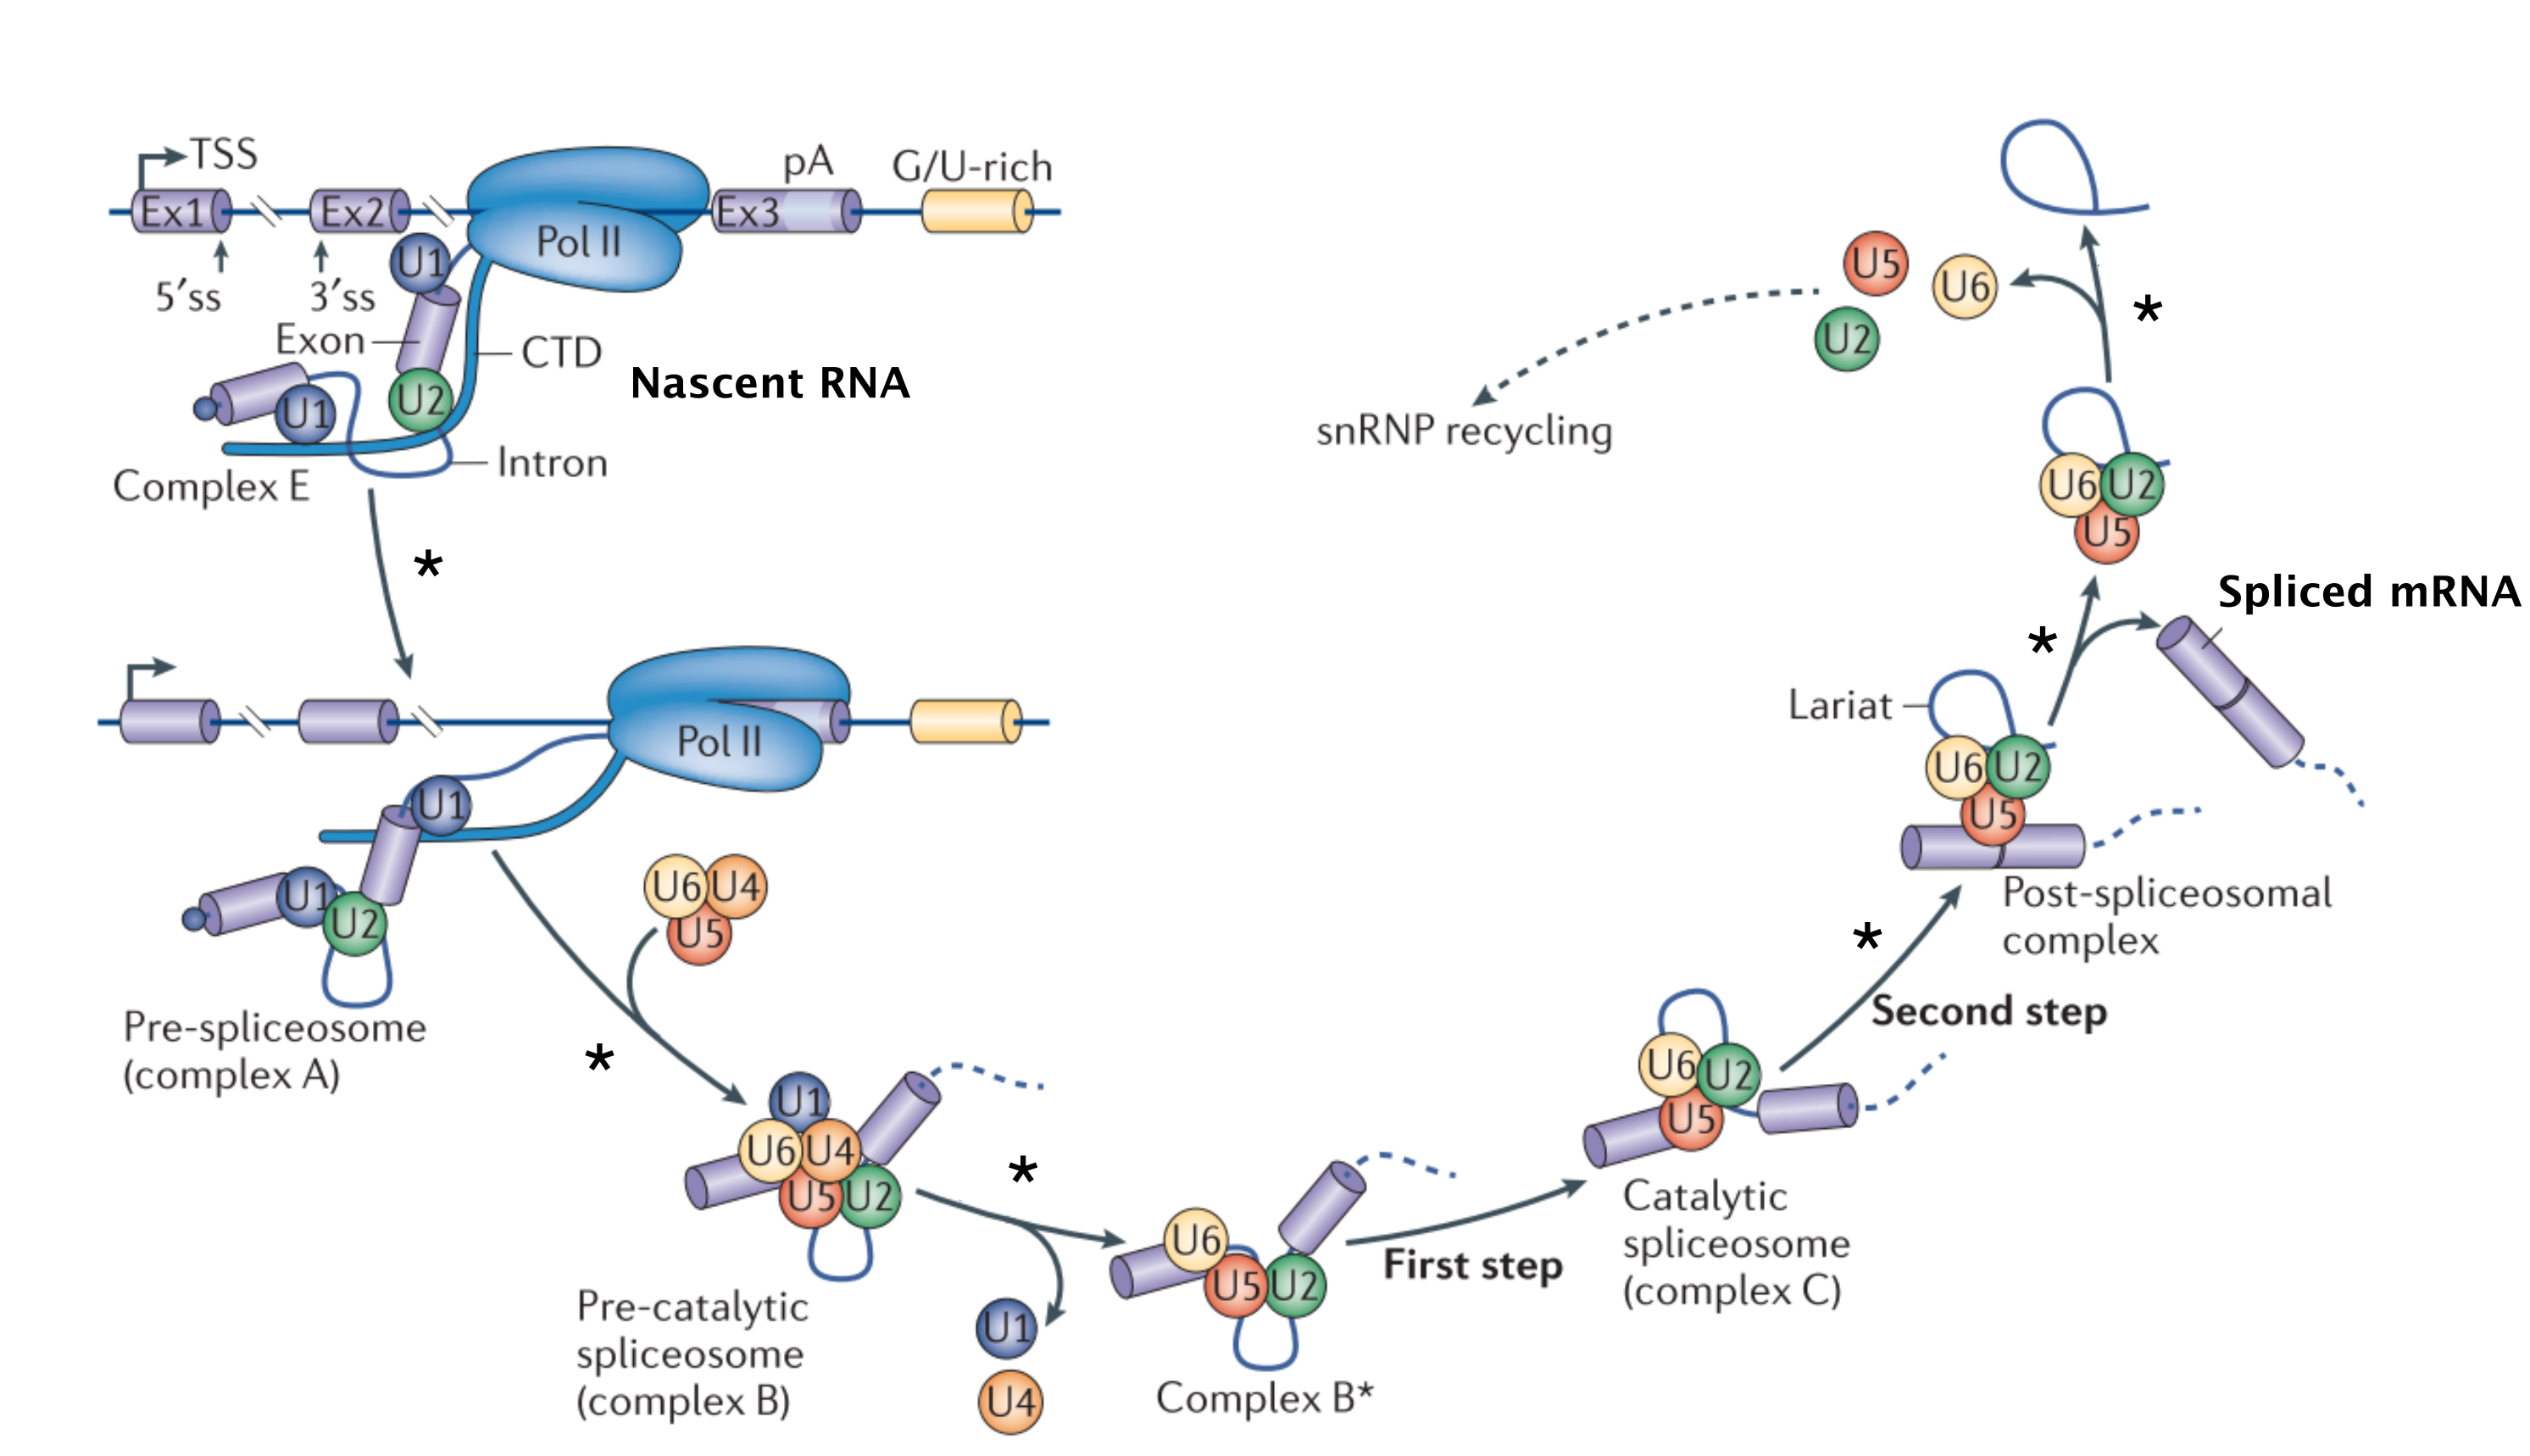
\includegraphics[width=\textwidth]{Figures/01_introduction/splicing.png}
	\caption[Splicing of a U2-dependent intron]{
		\textbf{Splicing of a U2-dependent intron.}
		Splicing proceeds through the recruitment of snRNP particles on the nascent RNA and the formation of different complexes, which transition through different arrangements. 
		* denotes the transition is dependent on the action of ATP and RNA helicases to proceed.
		Figure taken from \citep{Matera2014}. Names of specific helicases have been removed for simplicity.
	 }
	\label{fig:intro_splicing}
\end{figure}

The discovery of a large discrepancy between the length of a gene and the length of its mRNA ushered in new paradigm for biology: RNA splicing \citep{Berget1977,Chow1977}.
This is in essence a process of distinguishing which sections of a nascent RNA molecule are to be kept (the exons), and which are to be removed (the introns) to create a final transcript.
The majority of protein-coding genes are made up of multiple exons and so require splicing for the creation of their mature mRNAs. 
Beyond this, 95\% of multi-exon genes are alternatively spliced \citep{Pan2008,Wang2008}. 
Alternative splicing is the process where a particular set of exons in a gene are selected to be spliced together.
For protein-coding genes this is mechanism for creating functional diversity in the proteome, where a single gene can encode multiple proteins with different functions.
This has consequences for understanding gene regulation and cell biology.

Splicing depends on the reliable recognition of exons and subsequent removal of introns by the spliceosome complex. 
The spliceosome is a dynamic molecular machine made up of small nuclear ribonucleoprotein (snRNP) complexes containing small nuclear RNAs (snRNA) and their partnering proteins \citep{Matera2014}. 
Splicing proceeds by a set of interactions between the nascent RNA and the snRNP complexes (Fig. \ref{fig:intro_splicing}).
Eukaryotes have two types of introns which are spliced by separate groups of snRNPs: major or U2-dependent introns, and minor or U12-dependent introns. 
Major introns make up 99.5\% of human introns. I will describe the process of U2-dependent intron splicing.

snRNAs form base-pairing interactions with consensus RNA sequences called splice sites. 
These demarcate the boundaries between introns and exons. 
The 5\'\ splice site is recognised by the U1 snRNP and the 3\'\ splice site and the upstream branch point sequence is recognised by the U2 snRNP.
U1 snRNP binding precedes the U2 snRNP and the two complexes first pair together across an exon in a process known as exon definition. 
This is due to the long length of introns in higher eukaryotes that immediate pairing across the intron is unfavoured.
This complex transitions to an intron-defined arrangement across the adjacent intron which brings the two splice sites and the branch point into close contact.
At this point the U4/5/6 tri-snRNP is recruited and through a set of ATP-dependent rearrangements the spliceosome catalyses two transesterification reactions to remove the intron and join the two exons together.
The intron is circularised at the branchpoint to form a lariat structure which is then degraded.

% RBPs and alternate splicing
During splicing, other sequences in the nascent RNA can recruit RNA-binding proteins to modulate splicing by promoting or repressing the splicing of particular exons.
This is the mechanism behind alternative splicing and is an interplay between the \textit{cis}-acting RNA sequence and \textit{trans}-acting proteins.
Whether an exon is included in a mature mRNA transcript depends on the local environment around the splicing reaction.
Sequence motifs can be classified based on which factors they recruit and by what the result of binding is, whether binding enhances or silences the splicing of the exon.
Therefore a motif in an exon that promotes its inclusion is an exonic splicing enhancer element. 
Whether a sequence is used to silence or enhance the splicing of an exon depends on its location within the exon-intron structure.
For example, the neuro-oncological ventral antigen (NOVA) proteins have a binding preference for YCAY sequences, where Y indicates a pyrimidine \citep{Buckanovich1996,Jensen2000}.
NOVA binding directly immediately downstream or distally upstream of an exon acts to promote its inclusion, whereas binding directly on top of an exon or adjacent to the upstream exon promotes exon skipping \citep{Ule2006}.
Multiple splicing factors can bind the same sequence elements and function as a network depending on their levels of expression \citep{Wang2013a}.
These splicing networks can be created by protein-protein interactions between factors or through protein-RNA interactions whereby a splicing factor can control its own splicing and the splicing of other factors. 
Therefore different tissues or development time points can promote the splicing of particular sets of genes through changing the expression levels of different RNA-binding proteins.

% functional consequences of alternate splicing
The inclusion of a particular exon can have a wide range of consequences for an RNA molecule and its eventual protein, if it is to be translated. 
The inclusion of an alternative or cassette exon may alter stability, add a new functional domain, change localisation or change protein-protein interactions.
One way the splicing can alter RNA stability is through the PTC-NMD pathway.
Exons can destabilise their host transcript by introducing premature termination codons (PTCs), stop codons that appear upstream of the final stop codon. 
These can make a transcript sensitive to degradation by the nonsense-mediated decay (NMD) pathway \citep{McGlincy2008-wh}. 
This occurs during the pioneer round of translation, where the ribosome detects a stop codon appearing before the final exon junction, which is demarcated by the exon-junction complex.
This triggers degradation.  % ref?
Intriguingly, splicing factors themselves often have NMD-sensitive isoforms \citep{Ni2007}. 
The splicing of NMD-sensitive isoforms in a splicing factor transcript is often triggered by the binding of that same splicing factor protein \citep{Jangi2014a}. 
This is a mechanism by which splicing factors regulate their own translation: a phenomenon known as autoregulation \citep{Rosenfeld2002}.

% co-transcriptional splicing
Splicing generally occurs as the nascent RNA is being transcribed by RNA polymerase II \citep{Beyer1988,Ameur2011}.
This allows for interaction behind the transcription and splicing machinery.
Two reciprocal models for this have been proposed: a recruitment model, where RNA motifs recruit splicing factors which themselves recruit transcriptional modifiers, and a kinetic model, where the modulation of elongation speed alters this recruitment by changing the availability of RNA motifs for recruitment \citep{Kornblihtt2004a}.
Alternate exons have weaker splice sites, whose sequence deviates from the high affinity consensus sequence \citep{Stamm2000}.
Pausing or slowing transcription speed can allow these weaker splice sites to be recognised and compete with stronger constitutive splice sites to promote alternate exon inclusion.
Alternatively, more time can allow for low-affinity silencing elements to be used to promote exon skipping.
A number of exons sensitive to transcription speed are found in genes for splicing factors \citep{Ip2011}, suggesting deep connections between transcription and splicing. 

% localise the problem to neurons
Of all the cells in the human body, neurons arguably make the largest demands upon the transcription and splicing machinery. Neuron-specific genes tend to be much longer than in other tissues \citep{Sibley2015} and an individual neuronal gene can be processed by alternate splicing to create 1000s of mRNA and subsequent protein isoforms \citep{Treutlein2014}. 
The distinct compartments of a neuron's architecture requires exquisite fine-tuning of protein function to suit its location, for example on either side of a synapse. 
There is also the matter of transport. 
Motor neurons can have axons over a metre long, along which an mRNA would have to travel to reach ribosomes close to a synapse for local translation. 
Small defects in splicing could have catastrophic consequences for neurons and motor neurons in particular. 

% long introns and cryptic exons
One example of neuronal vulnerability to splicing dyregulation is the phenomenon of cryptic exons.
Due to the reduced evolutionary conservation of intronic sequence, pairs of 3\'\ and 5\'\ splice sites can emerge randomly to create new exons, with long neuronal introns being most vulnerable. 
These cryptic exons (also known as pseudoexons) can arise due to mutations that create new splice sites or remove the existing binding sites for splicing repressors. 
These type of mutations have been implicated in a number of genetic diseases \citep{Eng2004-lq, Buratti2007-iz, Vorechovsky2006-wb,Meili2009-hc}. 
Inclusion of a cryptic exon, untested by evolution, can destabilise its host transcript or radically alter the eventual protein structure. 

% cryptic exons
Another source of cryptic exons are transposable elements. 
One such example are Alu elements, the predominant transposable element in primates which are often found within introns in the antisense direction \citep{Deininger2011-hc}. 
The consensus Alu sequence consists of two arms joined by an adenine-rich linker ending with a poly-adenine tail.  
When transcribed in the antisense direction these uridine-rich sequences can act as cryptic polypyrimidine tracts and only a few mutations are required to convert them into viable exons in a process termed exonisation \citep{Sorek2002-cm}.
\textit{De novo} mutations that lead to Alu exonisation have been found in a range of diseases \citep{Vorechovsky2010-or} suggesting a need for regulation of potentially damaging Alu exons. 
Alu exonisation is repressed by the RNA binding protein hnRNP C, which competes with the spliceosome component protein U2AF65, the partner of the U2 snRNA, for binding cryptic 3\'\ splice sites \citep{Zarnack2013}. 
Due to the potentially negative effects of incorporation of new exons, recognition of cryptic exons needs to be repressed. 
It is unknown how many other RNA-binding proteins play a role in repressing the recognition of cryptic splice sites.

% summarise
Splicing is a key biological mechanism for increasing protein function and regulating gene expression.
Studying RNA processing has been made substantially easier and more powerful by the emergence of new technology to survey the entire transcriptome at once: RNA sequencing.



\section{RNA-sequencing is a revolutionary technology to quantify gene expression and splicing} % the new hot method

RNA sequencing, henceworth written as RNA-seq, is the application of modern high throughput sequencing to directly determine the sequences and quantity of RNA molecules in a group of cells \citep{Wang2009}. 
Unlike the older microarray technology which relies on choosing a set of RNA probes to measure, RNA-seq is hypothesis-free. 
It is also highly sensitive, allowing for the detection of lowly expressed transcripts. 
Instead of measuring the intensity of a microarray probe, the abundance of a particular RNA molecule is calculated simply by counting the number of sequencing reads that contain its sequence. 
As sequencing technology has improved and reduced in cost, more complicated aspects of RNA regulation are now observable. 
Alternative splicing can be measured by the number of sequencing reads split across multiple exons: the splice junction. 
Complicated isoforms can be reconstructed from splice junctions where sequencing is sufficiently deep.

The real power of an RNA-seq experiment is that it is an open platform. 
Once the data is generated it can be downloaded and used in light of whatever the most up-to-date references, annotations or novel hypotheses happen to be. 
As it is now a requirement for publication that all raw sequence data is made available, this allows for large scale re-analysis and meta-analysis in light of new discoveries and ideas. 
Throughout my work I capitalise on this by re-analysing public datasets and combining their results to find new and interesting biology.
This ease of replication is a triumph for modern science and will hopefully lead to more robust findings.


\section{RNA-binding proteins implicated in ALS/FTD}

The RNA hypothesis of ALS and FTD has emerged from evidence from pathology and genetics that centres around RNA-binding proteins, chief among them TDP-43 and FUS.
My work attempts to better understand the biological roles of these two proteins and link them to animal models of disease.

\begin{figure}[h!]
	\centering
	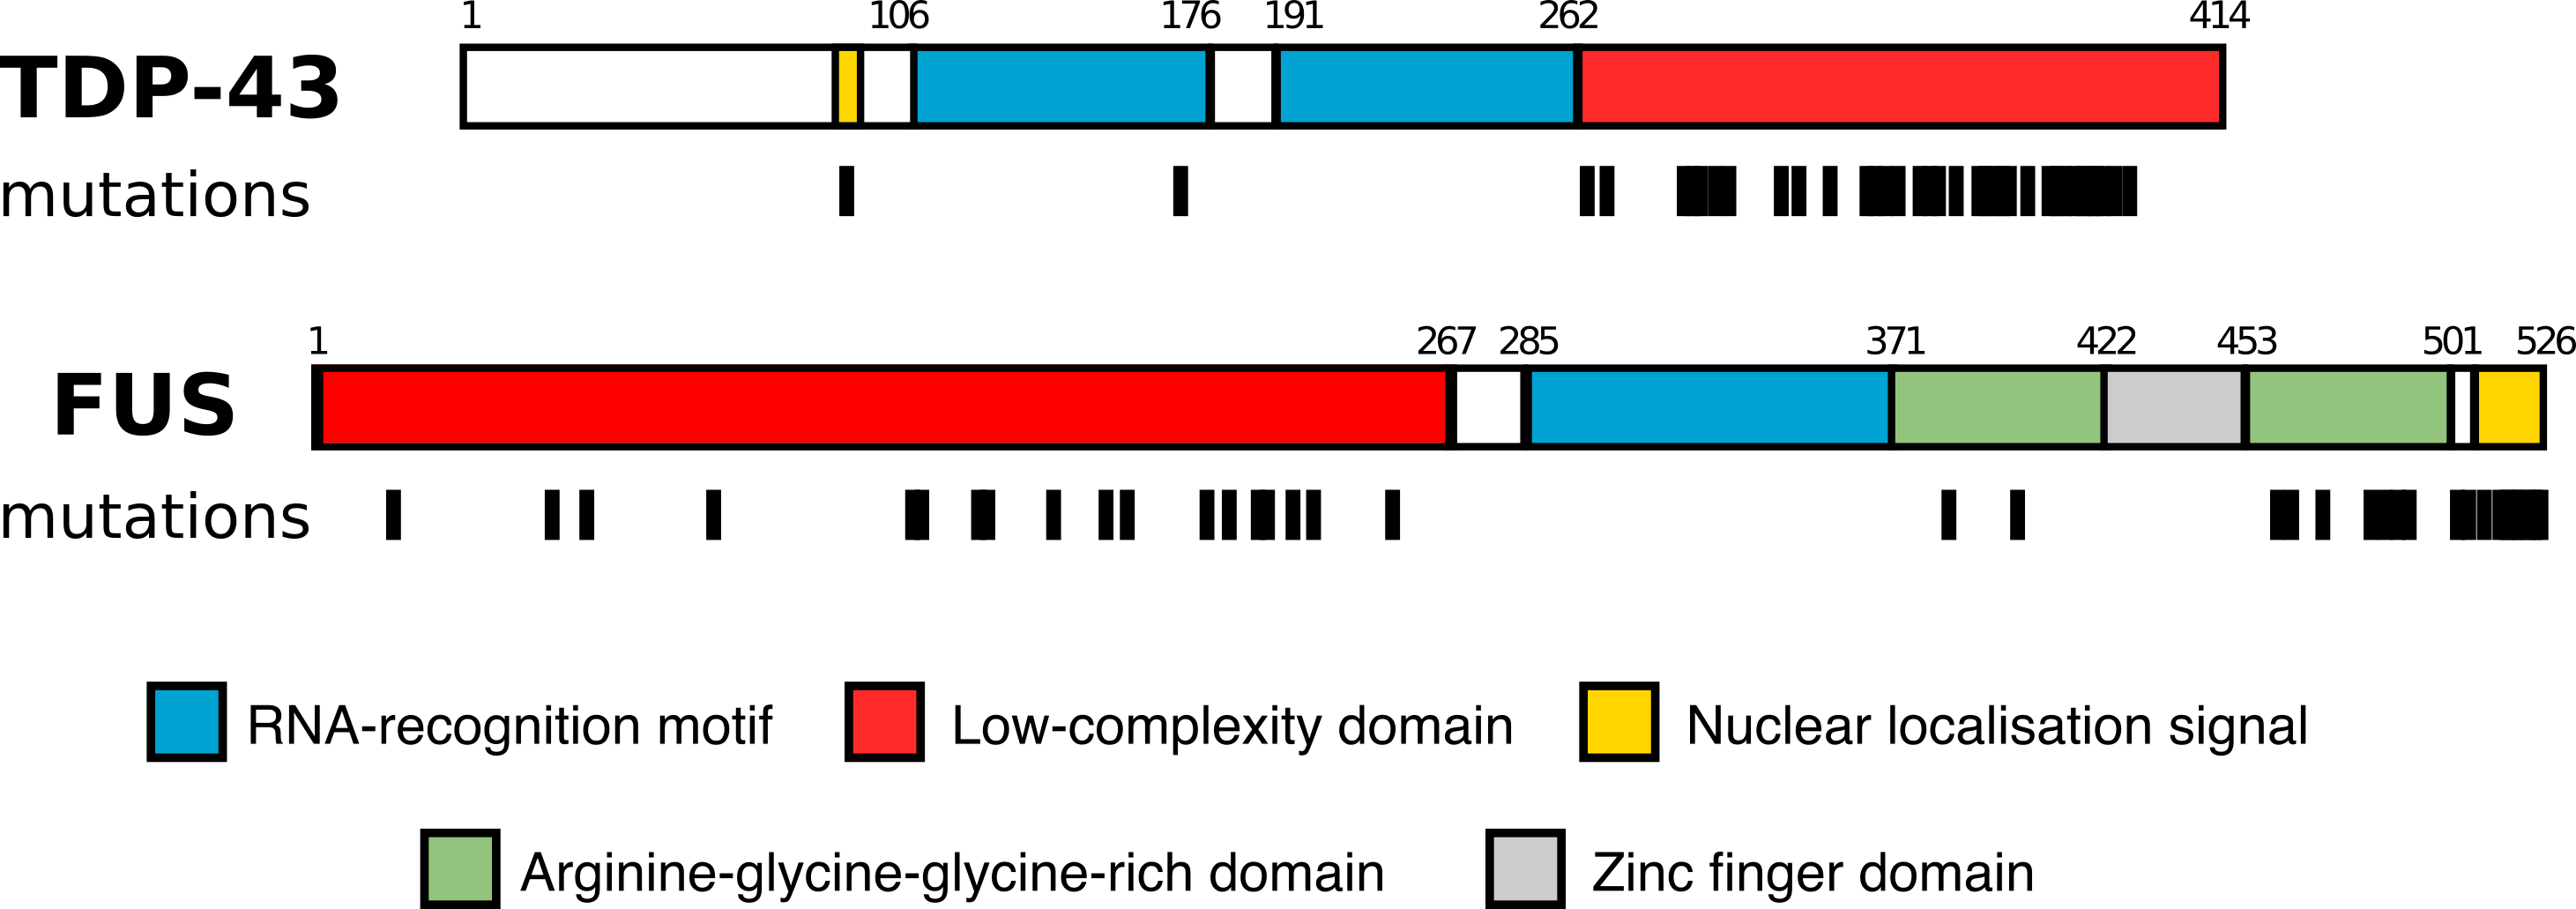
\includegraphics[width=\textwidth]{Figures/01_introduction/tdp_fus_structures.png}
	\caption[Protein domains of TDP-43 and FUS]{
		\textbf{Protein domains of TDP-43 and FUS}. Structures of the two proteins, coloured by functional domain. Positions of each mutation are represented by black bars. Figure adapted from \citep{Kapeli2017}. 
	}
	\label{fig:intro_domains}
\end{figure}


\subsection{TDP-43}

% intro
Transactive response DNA-binding protein 43 kDa (TDP-43) is a ubiquitously expressed RNA and DNA-binding protein encoded by the \emph{TARDBP} gene. 
It contains two RNA-recognition motifs, a nuclear localisation signal and a long glycine-rich low-complexity domain (Fig \ref{fig:intro_domains}).
Loss of TDP-43 from the nucleus accompanied by TDP-43 positive inclusions in the cytoplasm of cortical and spinal cord neurons is the hallmark pathology found in nearly all sporadic cases of ALS as well as the majority of non-Tau cases of FTD \citep{Neumann2006,Arai2006} as well as cases of Alzheimer's disease \citep{LaClair2016} and Huntington's Disease \citep{Doi2008}. 
Cytosolic TDP-43 has also been found in mouse models of traumatic brain injury, suggesting mislocalisation is a general neuronal stress response \citep{Moisse2009}. 
In addition, missense mutations in \emph{TARDBP} have been shown to cause familial ALS \citep{Sreedharan2008-xv}.  Mutations cluster in the low-complexity domain \citep{Kapeli2017};(Fig. \ref{fig:intro_domains}).
These findings point to a key role of TDP-43 in the development of ALS/FTD. 
There is still much debate on whether the mislocalisation of TDP-43 plays a role in neurodegeneration through a loss of normal nuclear function or a gain of cytoplasmic function.  
A further question is the influence of rare mutations in the TDP-43 low-complexity domain and how they contribute to pathology.

\subsubsection{Roles in RNA regulation}

TDP-43 is a predominantly nuclear protein but can shuttle to the cytoplasm \citep{Ayala2008}. 
This has implicated it both in nuclear roles in transcription and splicing, but also in RNA transport and translation. 
In splicing, TDP-43 binds UG-rich RNA motifs \citep{Buratti2001a, Buratti2001}, validated by X-ray crystallography \citep{Lukavsky2013}. 
TDP-43 binding can either repress or enhance cassette exon splicing depending on the motif position, as was found for individual genes \citep{Mercado2005-js,Bose2008-du,Shiga2012-it}.
This was expanded genome-wide by RNA-protein interaction experiments to find RNA targets of TDP-43 and correlate TDP-43 binding with cassette exon splicing \citep{Polymenidou2011,Tollervey2011,Kapeli2016}. % RNA maps?
For cassette exons, TDP-43 binds on top of or close to exons which it represses and further away from the exons it enhances \citep{Tollervey2011}, similarly to NOVA proteins.
However, the majority of TDP-43 binding was found to be deep within introns and on 3' untranslated regions (3'UTRs).
Long intron genes were strongly downregulated under TDP-43 depletion \citep{Polymenidou2011}, suggesting an important role for TDP-43 in their splicing and stabilisation. 
TDP-43 knockdown was found to cause the emergence of a set of cryptic exons from poorly conserved introns \citep{Ling2015}, suggesting that intronic binding of TDP-43 acts to repress cryptic splice sites. 
Unlike hnRNP C this has not been linked to a particular class of retrotransposon element, despite TDP-43 being observed to bind a range of retrotransposons including Alu elements \citep{Li2012,Zarnack2013,Kelley2014}.
Attempts to correlate TDP-43's effect on the splicing of a gene with a change in the level of the subsequent protein have found few examples \citep{DeConti2015,Stalekar2015}.

In the cytoplasm TDP-43 binds a set of genes at the 3'UTR \citep{Colombrita2012} and can form cytoplasmic RNA granules which in neurons are transported along axons \citep{Alami2013, Fallini2012}. This gives TDP-43 a role in local translation.
TDP-43 has been shown to either repress or enhance the translation of a small number of target transcripts \citep{Majumder2012, Majumder2016, Neelagandan2018}.
In addition, many of the proteins identified to interact with TDP-43 are involved in translation \citep{Freibaum2010-hw}.
TDP-43 controls its own translation by autoregulation.
This is achieved by TDP-43 binding the 3'UTR of the \textit{TARDBP} transcript \citep{Ayala2011,Koyama2016}. 
Under conditions of cellular stress, translation is temporarily paused when actively translated mRNAs and RNA-binding proteins assemble into processing bodies and stress granules \citep{Anderson2008}. 
This assembly relies on protein-protein interactions between low-complexity domains of RNA-binding proteins.
TDP-43 is recruited to stress granules \citep{Colombrita2009} and ALS-linked mutations in the low-complexity domain increase this level of recruitment \citep{Liu-Yesucevitz2010}.
These granules can then rapidly disassemble once stress is stopped.

% other roles for TDP in RNA
%Other roles in RNA regulation have been observed for TDP-43, such as microRNA creation \citep{Kawahara2012} and the binding of retrotransposon elements 

\subsubsection{Roles in disease}

In affected neurons and glial cells with ALS/FTD, TDP-43 leaves the nucleus and forms protein aggregates in the cytoplasm \citep{Neumann2006}. 
Efforts in understanding TDP-43 in disease have looked at both loss and gain- of function, as well as the relevance of TDP-43 mutations to pathogenesis.

% TDP aggregates
TDP-43 aggregates contain fragments of the TDP-43 C-terminal as well as full length TDP-43 that are phosphorylated and ubiquitinated \citep{Neumann2006,Arai2006, Bosque2013, Hasegawa2008}.
These aggregates are toxic to neurons  \citep{Zhang2009} and also contain a number of other RNA-binding proteins \citep{Dammer2012}.
TDP-43 can spontaneously aggregate with itself, and mutations in the low complexity domain increase the propensity to do so \citep{Johnson2009}.
TDP-43 aggregates are types of amyloid \citep{Fang2014}, specific structures that are toxic to neurons and found in multiple neurodegenerative diseases.
The relationship between the dynamic role of TDP-43 in RNA granules, including stress granules, and the formation of toxic TDP-43 aggregates is not yet fully understood.

Global loss of TDP-43 is lethal in the mouse embryo \citep{Kraemer2010} and postnatal deletion leads to rapid death \citep{Chiang2010}. 
Conditional knockout of TDP-43 in mouse postnatal motor neurons causes a gradual degeneration of affected neurons and atrophy of muscle \citep{Iguchi2013}. 

Overexpression of wildtype human TDP-43 in mice caused motor neuron degeneration in the spinal cord and severe motor impairment in proportion to the dose of the transgene \citep{Wils2010, Shan2010}.
However toxicity caused by TDP-43 overexpression occurs in mice without the observation of TDP-43 aggregates \citep{Wegorzewska2009, Barmada2010}.
Conversely, wildtype human TDP-43 was not found to be toxic when expressed at a physiological level \citep{Arnold2013} and only the ALS-causing mutant forms were found to cause motor neuron degeneration. 
Again, this occurred without observed TDP-43 loss in the nucleus nor cytoplasmic aggregation. 
This works suggests that TDP-43 toxicity to neurons does not require TDP-43 aggregates to form.
Clearly neurons are very sensitive to the expression level of TDP-43 protein, and this is compounded by autoregulation. 
Therefore, any changes in TDP-43 protein levels through knockdown or over-expression will interfere with this feedback loop, making it hard to gauge the true expression change of a particular targeting strategy. 





%% what do I do about FUS here?
%Rare ALS-causing mutations have been found in another RNA-binding protein, FUS \citep{Vance2009-ye}, further raising the possibility that the impairment of RNA processing is a central cause of ALS.  TDP-43 and FUS have both been shown to bind a set of overlapping RNA targets \citep{Lagier-Tourenne2012-wa}.

%%TDP-43 and splicing
%%FIRST thing to be found on TDP-43. How much agreement between studies?

%"TDP-43 binds to (GU)16 repeats in apoA-II intron 2 and represses exon 3 splicing" \citep{Mercado2005}

%965 altered splicing events seen in adult mouse brain with TDP-43 depletion \citep{Polymenidou2011}
%%\citep{Tollervey2011} TDP-43 can bind within exons to repress them but can also bind up or downstream of them. Generally binding further away (up to 250nt from the exon) acts to enhance inclusion.
%
%Other splicing factors are perturbed in TDP-FTD \citep{Mohagheghi2015}: "the expression of hnRNPA1/A2 and PTB/nPTB is significantly altered in patients with frontotemporal dementiawith TDP-43-positive inclusions" A large number of splicing factors also alter the inclusion of SORT1 exon 17b.


%tDP-43 and POLDIP3 splicing - annotated exon 3 in POLDIP is enhanced by TDP, loss of TDP reduces the inclusion. Laser capture of neurons from ALS brain show a reduction in exon 3 containing POLDIP3. POLDIP3 involved in maintaining cell size. Exon3 lacking POLDIP3 cannot rescue cell size as well from POLDIP3 or TDP-43 knockdown. \citep{Shiga2012}.

%"Validation of the bona fide splicing events that are consistent data, both in neuronal and non-neuronal cell lines demonstrated that TDP-43 substantially alters the levels of isoform expression" in four genes but only in 2 these changes could also be confirmed at the protein level \citep{DeConti2015}. - Assessing splicing changes is hard and there is no guarantee that this leads to changes in protein level. 

%Repeat elements - dpn't put in introuction
%5




%%HERE is a bunch of different findings from TDP-43 animal models
%How does each support loss- or gain-of-function hypothesis?

%"knockout of transactive response DNA-binding protein 43 in mouse postnatal motor neurons using Cre/loxp system, progressive weight loss and motor impairment around the age of 60 weeks, and exhibited degeneration of large motor axon, grouped atrophy of the skeletal muscle, and denervation in the neuromuscular junction. The spinal motor neurons lacking transactive response DNA-binding protein 43 were not affected for 1 year, but exhibited atrophy at the age of 100 weeks; whereas, extraocular motor neurons, that are essentially resistant in amyotrophic lateral sclerosis, remained preserved even at the age of 100 weeks" \citep{Iguchi2013}

%"increased excitatory synaptic inputs and dendritic spine densities in early presymptomatic mice carrying a TDP-43Q331K mutation" \citep{Fogarty2016}

%"postnatal deletion of Tardbp in mice caused dramatic loss of body fat followed by rapid death. Moreover, conditional Tardbp-KO ES cells failed to proliferate" \citep{Chiang2010}

%"mice expressing a mutant frm of human TDP-43 develop a progressive and fatal neurode- generative disease reminiscent of both ALS and FTLD-U. Despite universal transgene expression throughout the nervous system, pathologic aggregates of ubiquitinated proteins accumulate only in specific neuronal populatioons, including layer 5 pyramidal neu- rons in frontal cortex, as well as spinal motor neurons, recapitu- lating the phenomenon of selective vulnerability seen in patients with FTLD-U and ALS. Surprisingly, cytoplasmic TDP-43 aggregates are not present, and hence are not required for TDP-43-induced neurodegeneration." \citep{Wegorzewska2009} Overexpression of mutant human TDP A315T in mice at levels "3-fold higher" 

%"Mice expressing hu- man TDP-43 in neurons exhibited growth retardation and prema- ture death that are characterized by abnormal intranuclear inclusions composed of TDP-43 and fused in sarcoma/translocated in liposarcoma (FUS/TLS), and massive accumulation of mitochon- dria in TDP-43-negative cytoplasmic inclusions in motor neurons, lack of mitochondria in motor axon terminals, and immature neuromuscular junctions" \citep{Shan2010} 

%\citep{Igaz2011} "Expression of either hTDP-43-ΔNLS or hTDP-43-WT led to neuron loss in selectively vulnerable forebrain regions, corticospinal tract degeneration, and motor spasticity recapit- ulating key aspects of FTLD and primary lateral sclerosis. Only rare cytoplasmic phosphorylated and ubiqui- tinated TDP-43 inclusions were seen in hTDP-43-ΔNLS mice"

%"Two ALS-causing mutants (TDP-43Q331K and TDP-43M337V), but not wild-type human TDP-43, are shown here to provoke age-dependent, mutant-de- pendent, progressive motor axon degeneration and motor neu- ron death when expressed in mice at levels and in a cell type- selective pattern similar to endogenous TDP-43. Mutant TDP-43-dependent degeneration of lower motor neurons occurs without: (i) loss of TDP-43 from the corresponding nuclei, (ii) accumulation of TDP-43 aggregates, and (iii) accumulation of insoluble TDP-4" \citep{Arnold2013}




%tTDP-43 regulates the levels of other neurodegenerative disease mRNAs like FUS and PGRN \citep{Polymenidou2011} and preferentially stabilises the expression of long intron genes, something shared with FUS. iCLIP of TDP-43 showed "unusually long clusters of TDP-43 binding at deep intronic positions downstream of silenced exons." \citep{Tollervey2011}.

%tTDP-43 and UG motifs: "TDP-43 has a unique capacity to recognize dispersed clusters of UG-rich motifs, or to spread its RNA binding to positions proximal to the UG-rich motifs" \citep{Tollervey2011} Both RRMs come together to bind UG-rich RNA \citep{Lukavsky2013} - interactions between the two RRMs are crucial for RNA binding




%%OTHER stuff TDP does


%%RNA transport
%\citep{Alami2013} finds "TDP-43 is a component of mRNP transport granules in neurons, including human stem cell-derived motor neurons, and identify a new role for TDP-43 in the cytoplasm supporting anterograde axonal transport of target mRNAs from the soma to distal axonal compartments"

%%TDP-43 autoregulation 
%first seen by Polymenidou \citep{Polymenidou2011} then assessed by \citep{Ayala2011} \citep{Er??ndiraAvenda??o-V??zquez2012} and \citep{Koyama2016}. TDP-43 binds the 3'UTR of the TARDBP mRNA to prevent the usage of the proximal polyA site. The longer TARDBP 3'UTR transcript undergoes multiple splicing rounds that ultimately reduce the levels of TDP-43 protein. With TDP-43 depletion the proximal polyA site is used and the levels of cytoplasmic TARDBP mRNA are increased.

%%TDP-43 proteomics
%proteomic study on loss of TDP-43 \citep{Stalekar2015} "TDP-43 is an important regulator of RNA metabolism and intracellular transport."
%%TDP interactome \citep{Freibaum2010-hw} shows TDP-43 interacts with multiple splicing factors (MATR3/hnRNPAB/SFPQ) as well as ribosomal proteins. "Disease-causing mutations in TDP- 43 (A315T and M337V) do not alter its interaction profile. TDP-43 interacting proteins largely cluster into two distinct interaction networks, a nuclear/splicing cluster and a cytoplasmic/translation cluster, strongly suggesting that TDP-43 has multiple roles in RNA metabolism and functions in both the nucleus and the cytoplasm"

%Impaired nuclear import of WT TDP-43 as general mechanism
%Screen of 82 nuclear import proteins "knockdowns of karyopherin-b1 and cellular apoptosis susceptibility protein resulted in marked cyto- plasmic accumulation of TDP-43." \citep{Nishimura2010} "considerable reduction in expression of cellular apoptosis susceptibility protein in frontotemporal lobar degeneration."




%Prion-like C terminal 
%
%"TDP-43 does have inter-domain in- teractions which is coordinated by the intrinsically-disordered prion-like domain" \citep{Wei2016}
%
%Mitochondria
%%TDP-43 localises to the mitochondria of motor neurons and this increases with the increase in cytoplasmic TDP in ALS. TDP-43 mutations increase mitochondrial localisation. In mitochondria TDP binds complex I components TDP-43 protein sequence contains multiple mitochondrial import sequences. Competitive inhibition of TDP-43's mitochondrial localisation rescues neurotoxicity. \citep{Wang2016}
%
%
%%TDP depletion in Alzheimers - "TDP-43 proteinopathy, initially associated with ALS and FTD, is also found in 30–60\% of Alzheimer’s disease (AD) cases and correlates with worsened cognition and neurodegeneration." Some forebrain AD sensitive neurons are selectively vulnerable to TDP-43 loss.
%




% FUS


\subsection{FUS}

Fused in sarcoma is a ubiquitously expressed RNA-binding protein encoded by the \textit{FUS} gene. 
The FUS protein consists of a long low-complexity domain, an RNA-recognition motif, two arginine-glycine-glycine domains, a zinc finger domain and a N-terminal nuclear localisation signal (Fig. \ref{fig:intro_domains}).
%The previously identified nuclear export signal is in fact non-functional and FUS leaves the nucleus through passive diffusion \citep{Ederle2018}. 
FUS is a member of the FET family of RNA binding proteins, sharing high sequence homology with EWSR1 and TAF15 \citep{Kovar2011}.
Mutations in \textit{EWSR1} and \textit{TAF15} have both been found in a small number of ALS patients \citep{Neumann2011, Couthouis2011,Ticozzi2011,Couthouis2012}.
Over 40 mutations in FUS have been found to cause ALS, accounting for around 5\% of familial cases and 1\% of sporadic cases \citep{Vance2009-ye,Kwiatkowski2009}.  
Mutations cluster in the low complexity domain and the nuclear localisation signal.
FUS-ALS is distinguished from sporadic ALS by its aggressive early onset and the presence of FUS protein in cytoplasmic aggregates and not TDP-43. 
FUS mutations have also been found in a very small number of FTD cases \citep{VanLangenhove2010,Broustal2010}.
However, FUS-positive inclusions are seen in around 10\% of FTD cases in the absence of any FUS mutation \citep{Neumann2009}. 
Additionally, FUS has also been detected in aggregates from cell and mouse models of Huntington's disease \citep{Doi2008, Kino2016}.

\subsubsection{Roles in RNA regulation}

Although predominantly localised to the nucleus, FUS appears have a role in every step of RNA processing in both the nucleus and cytoplasm. 
As a splicing factor it binds to GGU motifs within introns and 3' UTR sequences to either enhance or repress exon inclusion and polyadenylation \citep{Rogelj2012,Lagier-Tourenne2012}.
As with TDP-43, FUS preferentially binds within introns and 3'UTRs \citep{Lagier-Tourenne2012,Rogelj2012,Ishigaki2012}. 
However the overlap between FUS and TDP-43 RNA targets is small  \citep{Lagier-Tourenne2012,Rogelj2012,Colombrita2012, Honda2014}.
A small number of genes were found to have FUS binding antisense to the promoter \citep{Ishigaki2012}.
In genes with long (>100kb) introns, FUS binding has a sawtooth pattern which appears to decline over the length of the intron \citep{Rogelj2012}. 
FUS depletion leads to downregulation of long intron genes \citep{Lagier-Tourenne2012}, suggesting FUS plays a role in stabilising the splicing of particularly long introns.
FUS also has a role in polyadenylation through its interaction with RNA polymerase II \citep{Schwartz2012} as it can stall transcription at 3'UTRs to encourage premature polyadenylation \citep{Masuda2015}. 
FUS has been observed to modulate 3' end processing of RNA, as observed in the GluA1 AMPA receptor subunit \citep{Udagawa2015}. % what does it modulate?
FUS knockdown has also shown to alter levels of intron retention, particularly in splicing factors \citep{VanBlitterswijk2013, Nakaya2013}.

In transcription, FUS interacts with RNA polymerase II, which could modulate transcription elongation speed \citep{Schwartz2012}.
FUS interacts with both the major spliceosome via the U1 snRNP \citep{Sun2015a, Yu2015a} and the minor spliceosome through binding to  the U11 snRNP \citep{Reber2016}, both of which define the 5' splice site at major or minor introns.
Within splicing factor networks FUS also interacts with TDP-43, MATRIN3, hnRNP A1, PTBP1 and other SR splicing factors \citep{Lagier-Tourenne2012,Yamaguchi2016,Yang1998,Meissner2003, Kamelgarn2016}. 
Some of these interactions are RNA-dependent \citep{Kamelgarn2016}.
The role of FUS in splicing is therefore highly complex and nuanced.

Beyond mRNA, FUS facilitates the creation of both microRNA \citep{Morlando2012} and circular RNA \citep{Errichelli2017}, two RNA species with complex regulatory functions.
In the cytoplasm FUS has also been observed in RNA transport granules \citep{Kanai2004, Fujii2005}.
FUS is also present in cytoplasmic SMN complexes which create the spliceosomal snRNP complexes  \citep{Yamazaki2012,Groen2013}.
% Stress granules
As with TDP-43, FUS aggregation has been linked to stress granule formation.
FUS itself is recruited into stress granules \citep{Andersson2008,Yasuda2013}. 
NLS mutations increase cytoplasmic FUS and increase FUS stress granule recruitment \citep{Dormann2010, Bosco2010}.
This requires RNA-binding activity of FUS to occur \citep{Daigle2013}	.
FUS aggregates found in ALS/FTD patients also contain stress granule proteins \citep{Dormann2010} suggesting a link between stress granule formation and disease.
Like TDP-43, FUS can control its own translation by autoregulation.
This is thought to occur by FUS binding creating an NMD-sensitive exon skipping isoform \citep{Zhou2013}.



\subsubsection{Roles in disease}

Although causative ALS mutations have been found throughout the FUS protein, mutations associated with the lowest age of onset and shortest disease course are clustered in the proline-tyrosine) nuclear localisation signal (NLS). 
Nuclear import of FUS is controlled by the nuclear import receptor protein Transportin binding to the NLS \citep{Dormann2010}.
The most aggressive FUS mutations either mutate the key proline residue in the terminal PY motif (P252L; \citep{Chio2009}) or remove the NLS entirely through a frameshift (G466VfsX14; \citep{DeJesus-Hernandez2010}) or a stop codon (R495X; \citep{Bosco2010}). 
Patients with these NLS ablating mutations tend to die in their early 20s whereas patients with NLS mutations further from the PY sequence have disease onsets resembling sporadic ALS \citep{Shang2016}.
The fact that most aggressive FUS-ALS mutations ablate the NLS suggests that mislocalisation of FUS in the cytoplasm is the key pathogenic event. However, whether this is due to a loss of nuclear FUS or toxic gain of function from the increased cytoplasmic FUS is still unclear.
Like TDP-43, FUS protein can spontaneously aggregate \textit{in vitro} through its low complexity domain \citep{Murray2017}. 
NLS mutations do not alter the propensity of FUS to self-aggregate \citep{Sun2011}.
Instead NLS mutations mislocalise FUS to the cytoplasm, which may encourage aggregation. The interaction between Transportin and the FUS NLS has recently been recognised to promote the dissolution of FUS aggregates \citep{Guo2018, Yoshizawa2018}. 
Reduced nuclear FUS would also impair autoregulation, increasing translation of FUS protein. This would then increase cytoplasmic FUS.
% animal models
In the mouse, complete knockout of endogenous FUS is lethal in an inbred C57BL/6 J background  \citep{Hicks2000, Kuroda2000} but survive until adulthood on a mixed background with no apparent motor deficits at 90 weeks of ages \citep{Kino2015}.
% overexpression
Overexpression studies have found a dosage dependence for the expression of human FUS to cause disease symptoms \citep{Verbeeck2012,Mitchell2013, Shiihashi2016}, with neurodegeneration and death only seen when human mutant FUS was highly expressed.
Overexpression of NLS mutant FUS does not appear to alter the splicing of FUS RNA targets \citep{Shiihashi2016}, despite mutant FUS interacting with the endogenous wildtype FUS \citep{Qiu2014}.
% gain of function
Other studies suggest a gain of function mediated by mutant FUS being responsible for neurodegeneration. 
Post-natal knockout of endogenous FUS  in motor neurons did not lead to motor dysfunction \citep{Sharma2016}.
A direct comparison between FUS knockout and mutation demonstrated embryonic lethality in both conditions, but with motor neuron loss only seen in the mutant mice \citep{Scekic-zahirovic2016}.  
There are still no mouse models of FUS ALS that study mutant FUS at a physiological expression level.



%of human FUS in mice causes a progressive motor neuron loss and death by 3 months, accompanied by cytoplasmic FUS protein expression \citep{Mitchell2013}. 
%This occured only when the FUS knockout transgene was homozygous, suggesting a dose sensitivity to the wildtype human protein for neurodegeneration. 
%
%Expression of mutant human FUS in the mouse brain caused an increased cytoplasmic accumulation of FUS relative to that of the wildtype, though no neurodegeneration was observed after 3months \citep{Verbeeck2012}. 
%
%Verbeeck and colleagues generated mice overexpressing FUS with either wildtype, an NLS mutation (R521C) or the NLS-ablating $\Delta14$ mutation \cite{Verbeeck2012}. Only mutant FUS was found to localise to the cytoplasm and the $\Delta14$ mutation also showed formation of cytoplasmic aggregates. 
%Overexpressing NLS-ablated FUS in mice leads to motor deficits and neuronal loss in motor cortex \citep{Shiihashi2016}. The authors did not observe any changes in FUS-mediated splicing activity.
%
%Overexpression of human FUS causes a progressive motor neuron loss and death by 3 months, accompanied by cytoplasmic FUS protein expression \citep{Mitchell2013}. 
%This only occurred when the FUS transgene was homozygous, suggesting a dose sensitivity to the wildtype human protein for neurodegeneration. 
%
%Qiu and colleagues created a transgenic mouse overexpressing R521C mutant FUS \citeyear{Qiu2014}. 
%They found that mutant FUS interacted with endogenous wildtype FUS and wildtype FUS protein is increased in the presence of mutant FUS. They also found neurodegeneration and DNA damage phenotypes, as well as widespread intron retention changes. 
%
%
%



\section{Aims of my PhD} 

% TDP and FUS biology - what do they do?

% TDP and FUS mouse models - how to better understand disease

Understanding the role of TDP-43 and FUS in disease requires studying their roles in neuronal cells.
The aim of my PhD is to capitalise on the RNA-seq revolution and bring together disparate datasets to assess the nature of RNA regulation by TDP-43 and FUS.
I can then apply that insight to novel animal models of disease generated by the UCL Institute of Neurology.


\section{Overview of chapters}

\subsection{Cryptic splicing occurs in published TDP-43 but not FUS depletion data}
TDP-43 has been observed to repress non-conserved intronic sequence from recognition by the spliceosome \citep{Ling2015}. 
I combined multiple public datasets on TDP-43 or FUS depletion and developed a method to discover and quantify cryptic splicing.
I expanded the number of cryptic exons found to be repressed by TDP-43 in human and mouse but did not find evidence of cryptic exon splicing in FUS.

\subsection{FUS mutant mice show progressive changes in mitochondrial and ribosomal transcripts}
Most attempts to model FUS ALS in mice either knock out endogenous FUS or over-express human mutant forms of FUS. 
Any study of RNA processing and/or motor neuron toxicity in these models is therefore confounded.
Dr Anny Devoy developed a new mouse model where an aggressive ALS mutation was knocked in to endogenous mouse FUS. 
This allows for the study of mutant FUS when expressed at a physiological level. 
I analysed RNA-seq data collected from two tissues and time points and observed a progressive change in mitochondrial and ribosomal transcripts restricted to the spinal cord.

\subsection{Loss and gain of TDP-43 splicing function in two mutant mouse lines}
ALS mutations in TDP-43 cluster in the C-terminal low-complexity region of the protein.
I studied RNA-seq datasets from two mutant mouse lines generated by random mutagenesis. 
One line had a mutation in the RNA-recognition motif which reduced the RNA-binding ability of TDP-43.
This was accompanied by cryptic exons, a sign of a loss of splicing function.
The second line had a mutation in the low-complexity domain.
I observed widespread skipping of normally constitutive exons, the inverse phenomenon to cryptic exon repression.

\subsection{ALS-causative FUS mutations impair FUS autoregulation through intron retention}
The most aggressive forms of ALS arise from mutations in the nuclear localisation signal of FUS.
I combined 3 embryonic mouse datasets where FUS was either knocked out or the nuclear localisation signal was removed.
This allowed me to jointly model the effects of the two different conditions, increasing detection power and confidence.
I observed substantial overlap in both gene expression and splicing, suggesting that the FUS mutations primarily reduce the nuclear function of FUS.
I identified a novel mechanism by which FUS could regulate its own translation.



% explain what RBPs do
% use examples from FUS and TDP-43 literature

% transcription

% splicing


% RNA transport

% Stress granules


%
%Introduce the two diseases. Introduce the RNA regulation theory of disease but also discuss the other possibilities

%Two bad neurodegenerative diseases
%Describe clinical presentations of both
%The ALS/FTD spectrum - linked through TDP-43 and FUS
%
%Evidence for RNA processing involvement in ALS/FTD
%
%
%%ALS/FTD and RNA-binding proteins


%In the case of TDP. FUS, A1/A2, Matr3, RBPs are mutated but with C9 RBPs are sequestered by the repeat. And yet all patients have similar phenotype.


% the biological problem
% from the paper:
%explain RNA regulation
%
%What do neurons need?
%Long genes with complex isoforms to increase protein diversity
%Need to transport RNA and protein over long distnace
%Local translation at synapses - control over protein expression


% progress in animal models of disease - put in discussion?
%The field as a whole is progressing towards more subtle and genuinely disease-like models; from the first knock-out mice, to over-expression of human mutant proteins to the more modern knock-in models where the mutant protein is expressed at a physiological level. While we can be more confident that the results from these more sophisticated experiments are closer to the the truth in humans, they suffer from a much longer generation time due to replicating diseases of old age. Changes in RNA may be subtler than we currently have the power to detect or more baroque than we can yet understand. 


% review of FUS functions citep{Ling2013}

%%FUS proteinopathies - citation?


%%TAF15 and EWSR1 share prion like domains with TDP-43 and FUS, missense variants in TAF15 in ALS patients \citep{Couthouis2011}
%%EWSR1 and TAF15 also in FTD-FUS cytoplasmic inclusions \citep{Neumann2011}
%variants in EWSR1 in ALS \citep{Couthouis2012}
%rare variants found in TAF15 in fALS causes \citep{Ticozzi2011-bs}


%Recent studies have demonstrated an interaction with RNA-polymerase II and the U1 snRNP \citep{Yu2015,Sun2015a}. 
%%SMN:
%"Expression of different FUS mutants (R521C, R521H, P525L) in neurons caused axonal defects. A protein interaction screen performed to explain these phenotypes identified numerous FUS interactors including the spinal muscular atrophy (SMA) causing protein survival motor neuron (SMN). Biochemical experiments showed that FUS and SMN interact directly and endogenously, and that this interaction can be regulated by FUS mutations" \citep{Groen2013}.
%"This studyshows that neuronal aggre- gatesformedbymutantFUSproteinmayaberrantlysequesterSMNandconcomitantlycauseareductionofSMN levels in the axon, leading toaxonal defects"
%
%It has also been linked to the minor splicesome \citep{Reber2016}. 
%
%Other roles for FUS:
%binding RNA polymerase II \citep{Schwartz2012}
%chromatin binding through binding to SAF3B and MATR3 \citep{Yamaguchi2016}
%regulates the expression of other RNA-binding proteins \citep{Nakaya2013}
%\citep{Rogelj2012}: binds GGU motifs within introns - less strongly than TDP-43 binds UG, represses inclusion of cassette exons, regulates splicing of Ewsr1 - same protein family as FUS. Genes with FUS-regulated splicing are enriched for neuronal development
%alternate polyadenylation \citep{Masuda2015} - position specific -  stalls RNA Polymerase II to initiate alternate polyadenylation of shorter transcripts
%
%Stress granules:
%	mutant FUS, but not wildtype FUS, forms stress granules in response to stress in Zebrafish \citep{Bosco2010}
%	"RNA-binding-deficient FUS strongly localized to the nucleus of Drosophila motor neurons and mammalian neuronal cells, whereas FUS carrying ALS-linked mutations was distributed to the nucleus and cytoplasm. Importantly, we determined that incorporation of mutant FUS into the SG com- partment is dependent on the RNA-binding ability of FUS" \citep{Daigle2013}
%
%\citep{Yasuda2013}: FUS recruited to APC-dependent granules which are translationally active, unlike stress granules. FUS promotes translation within these granules 
%
%Autoregulation:
%	\citep{Zhou2013} FUS binds its own introns to regulate its own expression - mutant FUS leaves the nucleus so cannot reduce its own expression levels - feedback. 

%
\chapter{A pipeline for RNA sequencing data analysis}
\label{chapter:methods}
% this should be for general methods 
% within each chapter I can talk about how I used these methods


The workhorse of my PhD is the processing of a large amount of RNA sequencing data, henceforth described as RNA-seq. To do so efficiently and effectively at scale requires a carefully thought out pipeline. Below I describe each section of the analysis pipeline collaboratively developed by the group of Vincent Plagnol but adapted and occasionally broken by myself. The pipeline is optimised for the UCL Computer Science cluster but is freely available to all from \url{github.com/plagnollab/RNASeq_pipeline/}

% insert flowchart of RNA-seq pipeline
\begin{figure}[h!]
	\begin{center}
		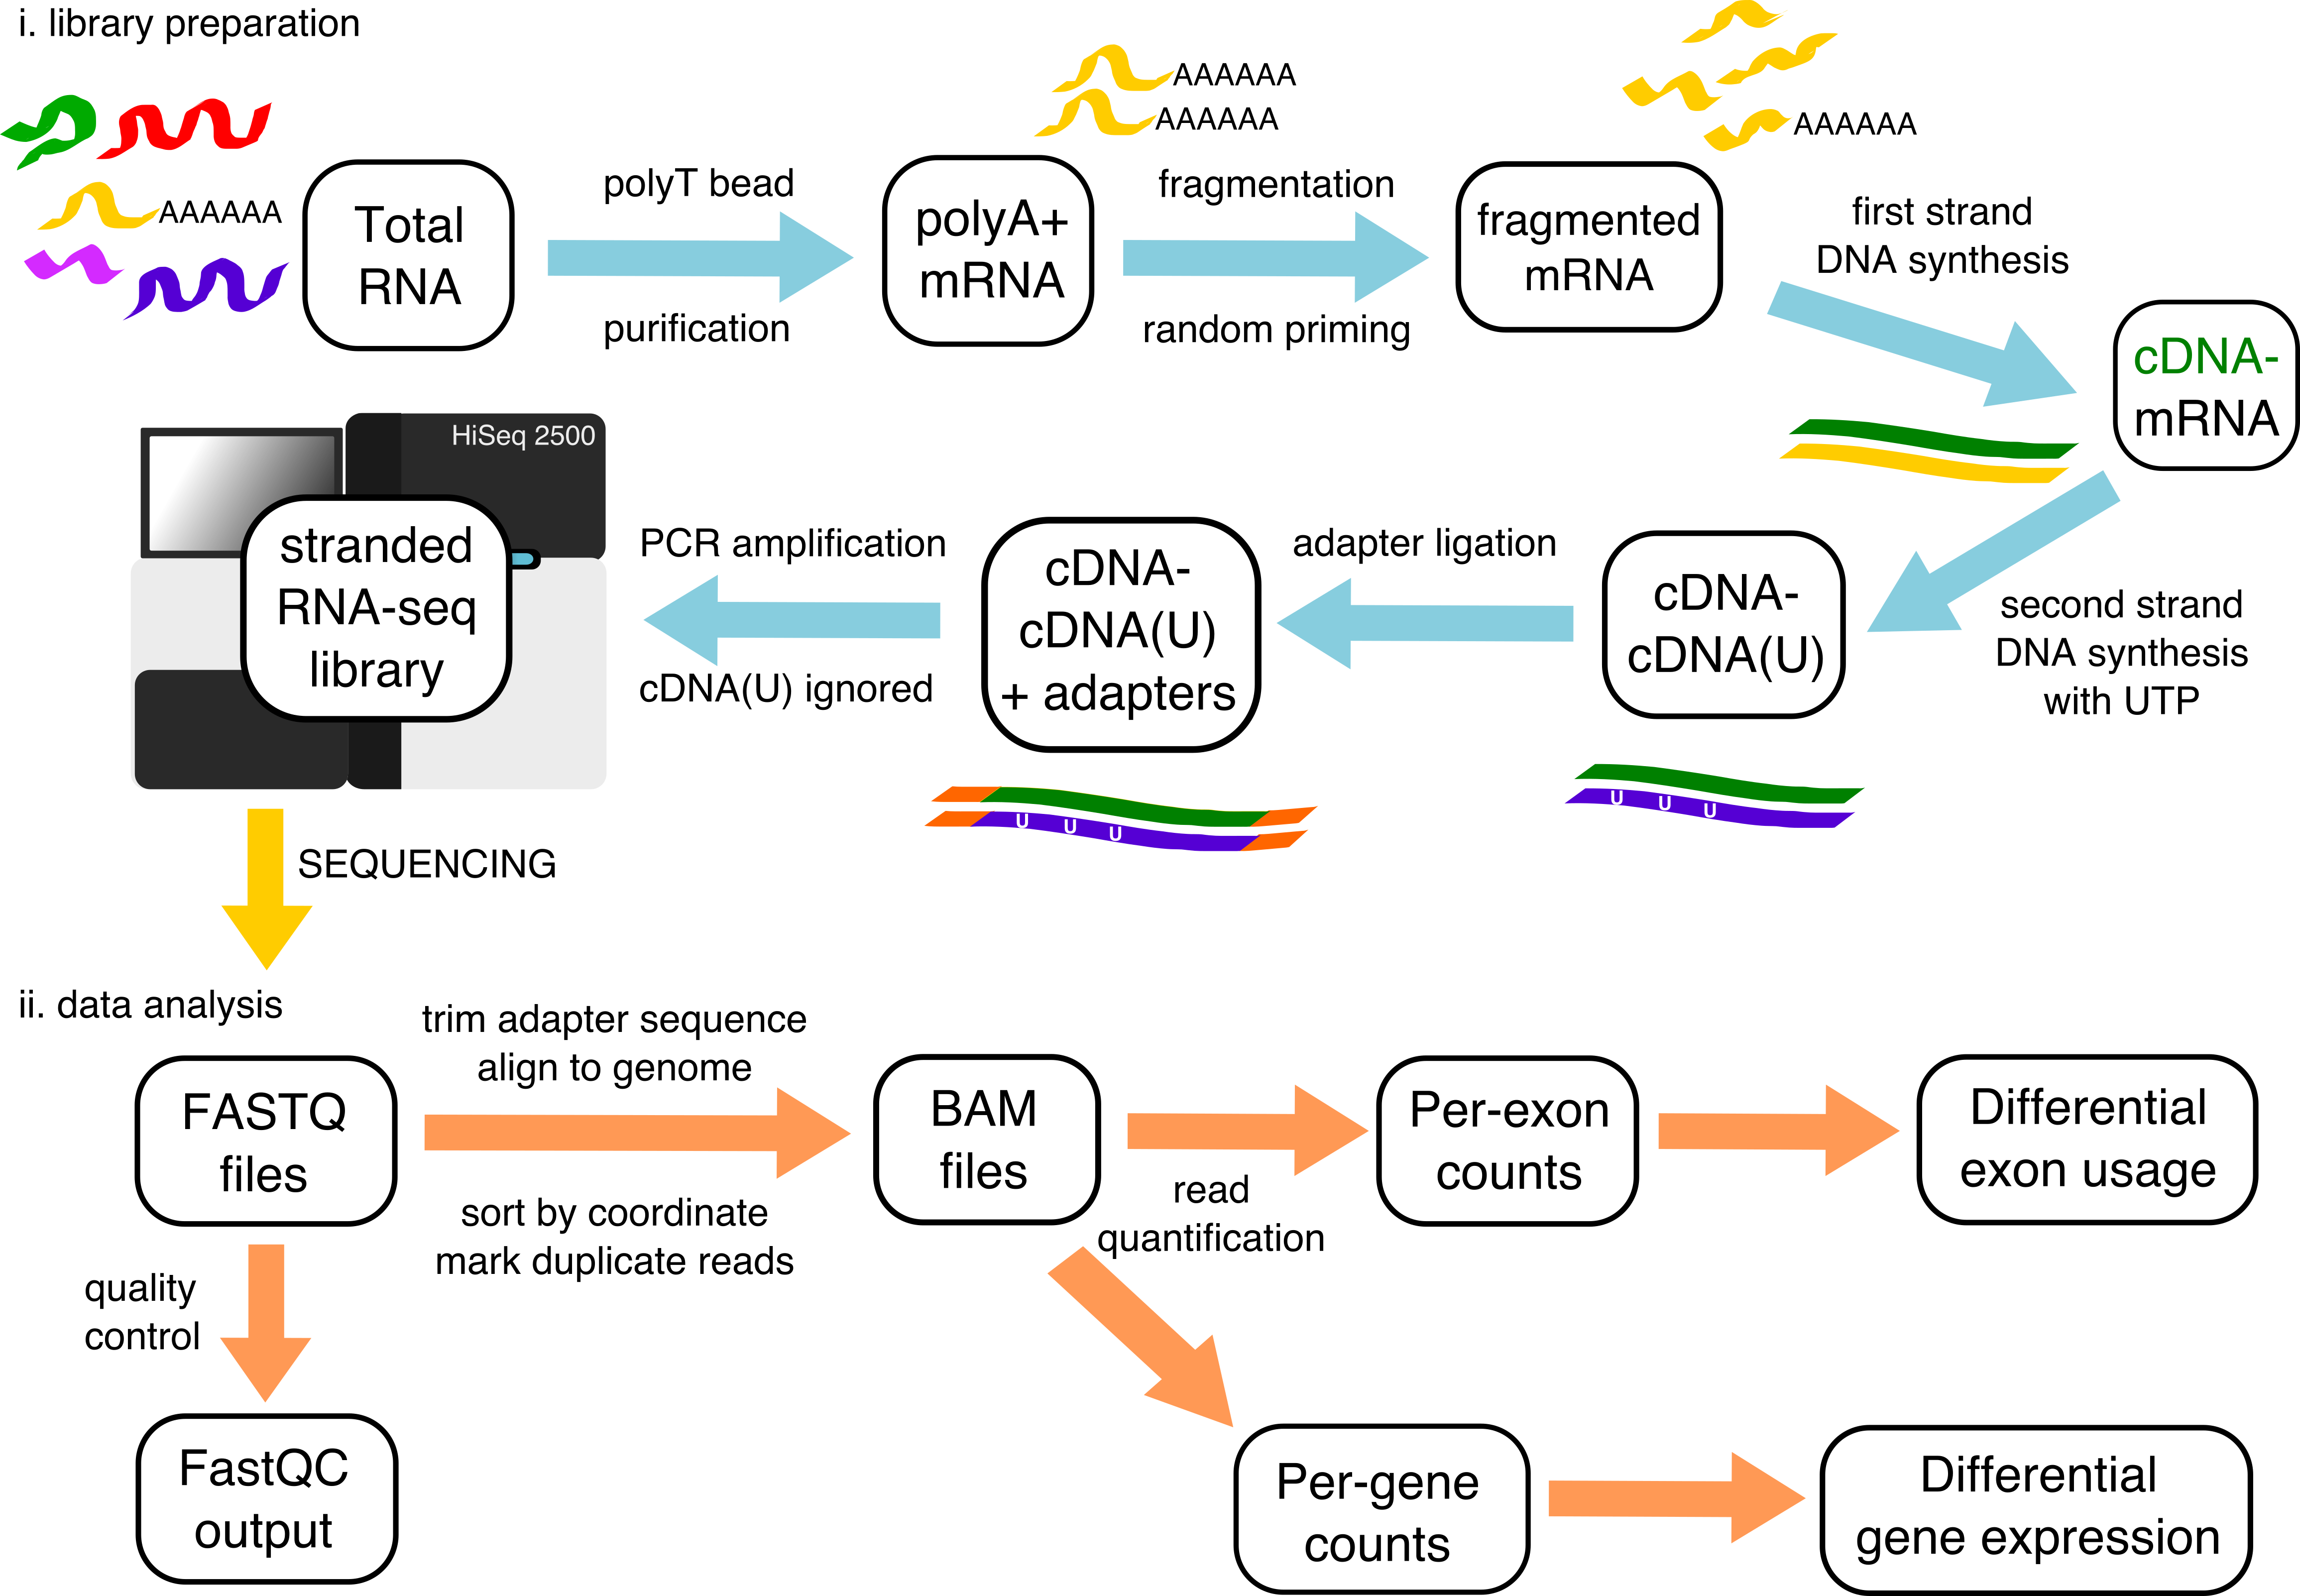
\includegraphics[width=14cm]{Figures/02_methods/RNAseq_pipeline_schematic.png}
	\end{center}
	\caption{Pipeline for stranded RNA-seq preparation and analysis}
	i) Library preparation from total RNA extraction and strand-specific amplification\\
	ii) Bioinformatic analysis workflow to align reads and test for differential gene expression and exon usage
\end{figure}

\section{Library preparation and sequencing}
I feel it is important to understand the preparation of a short read sequencing library so as to best interpret the data in downstream analyses. The description below is of a typical Illumina stranded RNA-seq library preparation.

Briefly, total RNA is extracted from cells or tissues using Trizol or a similar phenol/chloroform reagent \citep{Chomczynski1987}. The majority of RNA species in the cell are ribosomal RNAs. To enrich for mRNA species the RNA is mixed with magnetic beads that are bound to poly(Thymine) oligonucleotides, complementary to the poly(Adenine) tail at the 3' end of mRNA. The RNA is then fragmented. As paired-end sequencing extracts information from each end of the fragment it is important to consider the fragment size in light of the subsequent length of the reads, as with short fragments and long reads the read pairs will overlap leading to redundant information. Pseudo-random barcodes are ligated to each fragment to allow for reverse transcription. The first round of reverse-transcription is carried out forming double stranded DNA-RNA hybrids. These complexes are annealed and a second reverse-transcription reaction is carried out in the presence of Uracil instead of Thymine, creating double stranded DNA. The Uracilated DNA strand is now in the same orientation as the original mRNA fragment. Polymerase chain reaction amplification is then carried out where the uracil containing DNA and the RNA are ignored by the polymerase. The resulting library is strand-specific as all the DNA fragments are antisense to the original RNA fragments. Further adapters are added for sequencing in the flowcell and to give the fragments from each sample an identifier as multiple samples are usually pooled together. 
The standard Illumina paired-end sequencing reaction ligates the amplified fragments to wells in the flowcell which then form clusters of identical amplified fragments. Sequencing then occurs by sequential addition of fluorescent nucleotides along the length of a fragment in both directions, the  colour of which is recorded by a high resolution sensor. The identity of each nucleotide is determined and given a quality score based on the confidence of the measurement. The reads are converted to a FASTQ file, with separate files for the forward and reverse reads. This is a digital encoding of the sequence of both ends of each DNA fragment.

\section{Quality control and read alignment}
The first step in any analysis is quality control of the FASTQ files. Popular tools like \textit{FastQC} (\url{bioinformatics.babraham.ac.uk/projects/fastqc/}) analyse a set of FASTQ files and produce visualisations of multiple diagnostic tests. It can be useful to observe the range of quality scores and how they alter throughout the length of a read to diagnose faults during the sequencing reaction. Another important diagnostic is the presence of adapter sequences within reads. This can occur when the fragmentation step is too aggressive or when the original RNA sample is heavily degraded, often the case in human brain samples. With very short fragments, the sequential addition of nucleotides runs into the adapter sequence of the reads, making these reads much more difficult to align. These universal adapter sequences can be removed by software such as \textit{Trim Galore!} (\url{bioinformatics.babraham.ac.uk/projects/trim_galore/}), which can also remove low quality sequence from the ends of reads, which often occurs towards the end of a sequencing run. 

Following trimming, the FASTQ files must then be aligned to the genome of the species in question. There have been great advancements in speed and accuracy in alignment algorithms, but the key difference between DNA and RNA alignment is the need for read splitting. As most mRNAs are spliced, any RNA fragment that originates from the boundary between two exons will need to be split and both pieces separately aligned to the genome. The interval between two pieces is then recorded by the aligner as a splice junction, the demarcation of where an intron was excised. The current state-of-the-art algorithm in both speed and accuracy at resolving splice junctions is \textit{STAR} \citep{Dobin2013-ra}, which derives its speed from loading the entire genome into memory and then mapping millions of reads per hour using a seed-and-extend algorithm, where small pieces of each read are aligned and incrementally extended to find the best possible split alignment. The alignment information for each read is recorded in a BAM file. Reads from each pair are initially recorded next to each other and the BAM file is ordered by the read name. However for most downstream analyses the BAM file must be re-ordered by genomic position. Our pipeline does this using the \textit{Novosort} algorithm (\url{http://www.novocraft.com/products/novosort/}). 

Another potential issue in RNA-seq data, particularly in older data or from human brain-derived RNA, is a bias towards fragments from the 3' end of mRNAs. This can also occur due to mRNA degradation before the poly(Thymine) purification which will then bias the library to sequences closest to the bound polyadenylation site at the 3' end. This can be obvious when observing coverage across all genes with a diagnostic package such as \textit{QoRTS} \citep{Hartley2015a}. As most differential expression software assumes even coverage throughout a gene body, heavily degraded samples can skew the estimates of gene or exon expression.

For downstream expression analysis, the aligned reads are then quantified for a set of features. These features can either can be whole genes or individual exons. There are multiple annotations for the human and mouse genome for where the known genes and exons are but our pipeline uses the Ensembl transcript annotation as our reference \citep{Cunningham2015}. Reads that overlap each gene or individual exon are counted using \textit{HTSeq} \citep{Anders2015-wz}.


\section{Differential gene expression}
The most common application of RNA-seq is for an experiment comparing the abundances of different RNAs between conditions, for example between the knockdown of a particular gene and a control. These experiments should be made up of multiple biological replicates, where RNA libraries have been prepared from different organisms or cell culture samples under the same conditions. This is so a fair assessment can be made of the biological variation in RNA abundance within each condition. This is in comparison to technical replicates, where the same library is sequenced multiple times, which only tells you about the variance in the measurement. The still-expensive cost of sequencing usually limits a lab to sequence a small number of biological replicates, which limits one's statistical power to detect small variations in RNA abundance and the confidence in the truth of one's results. There are multiple algorithms to test for differential expression but we have settled on using the \textit{DESeq2} package for its statistical robustness and speed \citep{Love2014}.
Differential expression algorithms attempt to compensate for the small sample sizes by making use of the fact that each sequencing library measures the abundance of tens of thousands of genes. The number of reads generated by each library can be highly variable and so this is also accounted for. \textit{DESeq2} normalises the read counts for each gene in each sample by the size of each sample's library, a \textit{size factor}. It then assumes that the normalised read counts fit a negative binomial probability distribution. It then estimates the variance or dispersion in read count for each gene across the samples. To compensate for small sample sizes, which tend to give a very high estimate of dispersion, it compares the dispersion between all genes and shrinks the estimate to a local average dispersion based on genes expressed at a similar level. Using these shrunken dispersion estimates, the software then fits two generalised linear models: a null model where condition has no effect and an alternative model where the change in condition explains the change in gene expression. The two models are compared with a Wald test on which model fits the data better, computing a P-value. The P-values generated for each gene are adjusted to correct for multiple testing using the Benjamini-Hochberg procedure \citep{Benjamini1995}. The output of a differential expression analysis gives you both an adjusted P value for each gene and a $log_2$ of the fold change in expression between the two conditions to give you an estimate of the effect size. A positive fold change indicates an increase in the treatment versus the control. 

%%\section{Gene ontology analysis } % only keep in if I have to write up Anny's work
%%Using GOSeq to correct for length bias in RNA-seq gene ontology 

\section{Quantifying annotated splicing changes }
Following differential gene expression analysis, the next most popular use for RNA-seq is in understanding changes in splicing across conditions. This can be tackled with multiple approaches but one of the most widely used methods is differential exon usage analysis, which was made available by the \textit{DEXSeq} package \citep{Anders2012}. Rather than measuring the abundance of individual isoforms, \textit{DEXSeq} requires a flattened list of "union exons" which is a set of non-overlapping intervals for each exon from each annotated transcript in a given gene. RNA-seq seq reads can then be counted at each union exon. \textit{DEXSeq} then compares the \textit{size factor} normalised counts from each exon with the counts from all the exons in a gene and how they vary across biological conditions, again with the use of generalised linear model. 
The output of a \textit{DEXSeq} analysis is each union exon in a gene is given a $log_2$ fold change between conditions and an adjusted P value from the test. Although this output can be used to demonstrate whether differential exon usage occurs due a condition, it is inherently difficult to extract meaningful information about the underlying biology. A significant union exon may not correspond to real exon. Therefore, hits from \textit{DEXSeq} need to be closely analysed in the context of the gene they reside in. Chapter 5 discusses recent alternatives to \textit{DEXSeq}. 



%\chapter{Cryptic splicing occurs in published TDP-43 but not FUS depletion data}
\label{chapter:cryptic_exons}
%SORT OUT APPENDICES

This chapter has been published as \citep{Humphrey2017}. See appendices for full reproduction of the manuscript.

\section{Overview}
A recent paper \citep{Ling2015} demonstrated a novel RNA phenotype following the knockdown of the RNA-binding protein TDP-43 from mouse and human cell lines that they termed "cryptic exons". The first project of my PhD was to build a tool that could replicate these results in other previously published RNA sequencing datasets. In doing so I have extended the scale and understanding of cryptic exons and their relation to TDP-43. In addition, I have demonstrated a key difference between TDP-43 and FUS, as the knockdown of FUS does not result in a similar splicing phenotype.

\section{Background}

Recently, Ling and colleagues observed the inclusion of cryptic exons when TDP-43 was depleted in HeLa or mouse embryonic stem cells \citep{Ling2015}. These cryptic exons were shown to originate from poorly evolutionarily conserved sequence and shared no positions between the two species. These findings raise the possibility that impaired exon recognition contributes to TDP-43's role in ALS aetiology.

Given the intriguing possibility that impaired recognition of exons plays a causal role in ALS, I aimed at replicating and expanding the findings of Ling and colleagues. I first developed a quantitative genome-wide analysis pipeline to detect and classify cryptic splicing. I then applied this pipeline to seven datasets (four human and three murine models) to systematically quantify cryptic splicing alterations associated with depletion of TDP-43. In addition I investigated FUS in order to determine whether modulation of cryptic splicing was a common feature of RNA-binding proteins implicated in ALS. Furthermore I analysed hnRNP C, as it had been previously shown to repress cryptic exons originating from Alu repeat elements. Lastly, I used independent protein-RNA interaction datasets, conservation data, repeat element annotation and splice site scoring to investigate the potential mechanisms linking TDP-43 depletion with the cryptic exon phenomenon.

	
\begin{table}[h!]
	\caption{\textbf{List of accessions}}
	%\begin{centerline}
	\begin{footnotesize}
		\begin{tabular}{lllllll}
			%\centering
			Assay & Accession Code & Downloaded & Target & Cell/Tissue & Pubmed ID\\
			\hline
			RNA-seq & PRJNA282887 & SRA\footnotemark & TDP-43 & Mouse ES  & 26250685 \\
			RNA-seq & PRJNA282692 & SRA & TDP-43 & Human Hela & 26250685 \\
			RNA-seq & PRJNA127211 & SRA & TDP-43 & Mouse ES & 20660762\\
			RNA-seq & PRJNA141971 & SRA & TDP-43 & Mouse adult brain & 21358643 \\
			RNA-seq & ENCSR129RWD & ENCODE\footnotemark & control & K562 mRNA & -\\
			RNA-seq & ENCSR134JRE & ENCODE & TDP-43 & K562 mRNA & -\\
			RNA-seq & ENCSR372DZW & ENCODE & control & K562 total RNA & -\\
			RNA-seq & ENCSR455TNF & ENCODE & TDP-43 & K562 total RNA & -\\
			RNA-seq & PRJNA174534 & SRA & FUS & Mouse adult brain & 23023293 \\
			RNA-seq & ENCSR084SCN & ENCODE & control & K562 mRNA & -\\
			RNA-seq & ENCSR325OOM & ENCODE & FUS & K562 mRNA & -\\
			RNA-seq & PRJEB3048 & SRA & hnRNP C & HeLa & 23374342 \\
			iCLIP & 20100222\_LUjt3 & iCOUNT\footnotemark & TDP-43 & Mouse embryonic brain 1 & 22934129\\
			iCLIP & 20091102\_LUjt5	& iCOUNT & TDP-43 & Mouse embryonic brain 2 & 22934129\\
			iCLIP & 20100222\_LUjt3 & iCOUNT & TDP-43 & Human neural stem cells & 21358640\\
			iCLIP & 20101125\_LUjt8 & iCOUNT & TDP-43 & Human SH-SY5Y 1 & 21358640\\
			iCLIP & 20091102\_LUjt5 & icount.biolab.si & TDP-43 & Human SH-SY5Y 2 & 21358640\\
			eCLIP & multiple & ENCODE & Multiple RBPs & HepG2 and K562 & -
		\end{tabular}
	\end{footnotesize}
	%\end{centerline}
\end{table}

\footnotetext[1]{Sequence read archive: \url{www.ncbi.nlm.nih.gov/sra} }
\footnotetext[2]{Encyclopedia of DNA elements:  \url{www.encodeproject.com} }
\footnotetext[3]{iCOUNT iCLIP web server: \url{www.icount.biolab.si} }



\section{Methods}

\subsection{Data preparation}
Table 1 lists all the public data used in this study. All RNA-seq data was downloaded in the FASTQ format and processed using our RNA-seq pipeline (chapter 2).
Processed iCLIP peak data was downloaded from the iCOUNT server. Both the human and mouse TDP-43 iCLIP data have been previously published \citep{Tollervey2011,Rogelj2012}.

Processed eCLIP data (previously described by \citep{Van_Nostrand2016-su}) was downloaded from the ENCODE project. The narrowPeaks bed format was used with the first nucleotide of the cluster defined as the peak. Peak coordinates from iCLIP and eCLIP were converted to the hg38 and mm10 builds using the \emph{LiftOver} tool from UCSC. 

\subsection{Cryptic splicing definition}
I define cryptic splicing as the inclusion of sequence into mRNA transcripts that is not annotated by an existing database of known exons. 
Splicing aware alignment software such as \emph{STAR} \citep{Dobin2013-ra} cut short reads that originate from a spliced transcript and align the pieces separately, marking the distance between them as a splice junction. Splice junctions can be used to reaffirm known splicing patterns or infer novel splicing. I therefore base my computation of cryptic splicing as a relative increase in splice junctions that join known splice sites to unannotated positions within introns, with this increase correlating with the depletion of a particular RNA binding protein. 
Different repositories have differing levels of proof for annotating exons but I define an annotated exon as one listed in the Ensembl list of transcripts (release 82) \citep{Cunningham2015} which contains many more alternatively spliced exons than the RefSeq database \citep{Pruitt2014} but is still more conservative than the GENCODE database \citep{Harrow2012}.

\subsection{Cryptic splicing discovery with the \emph{CryptEx} pipeline}

\begin{figure}
	\centering
	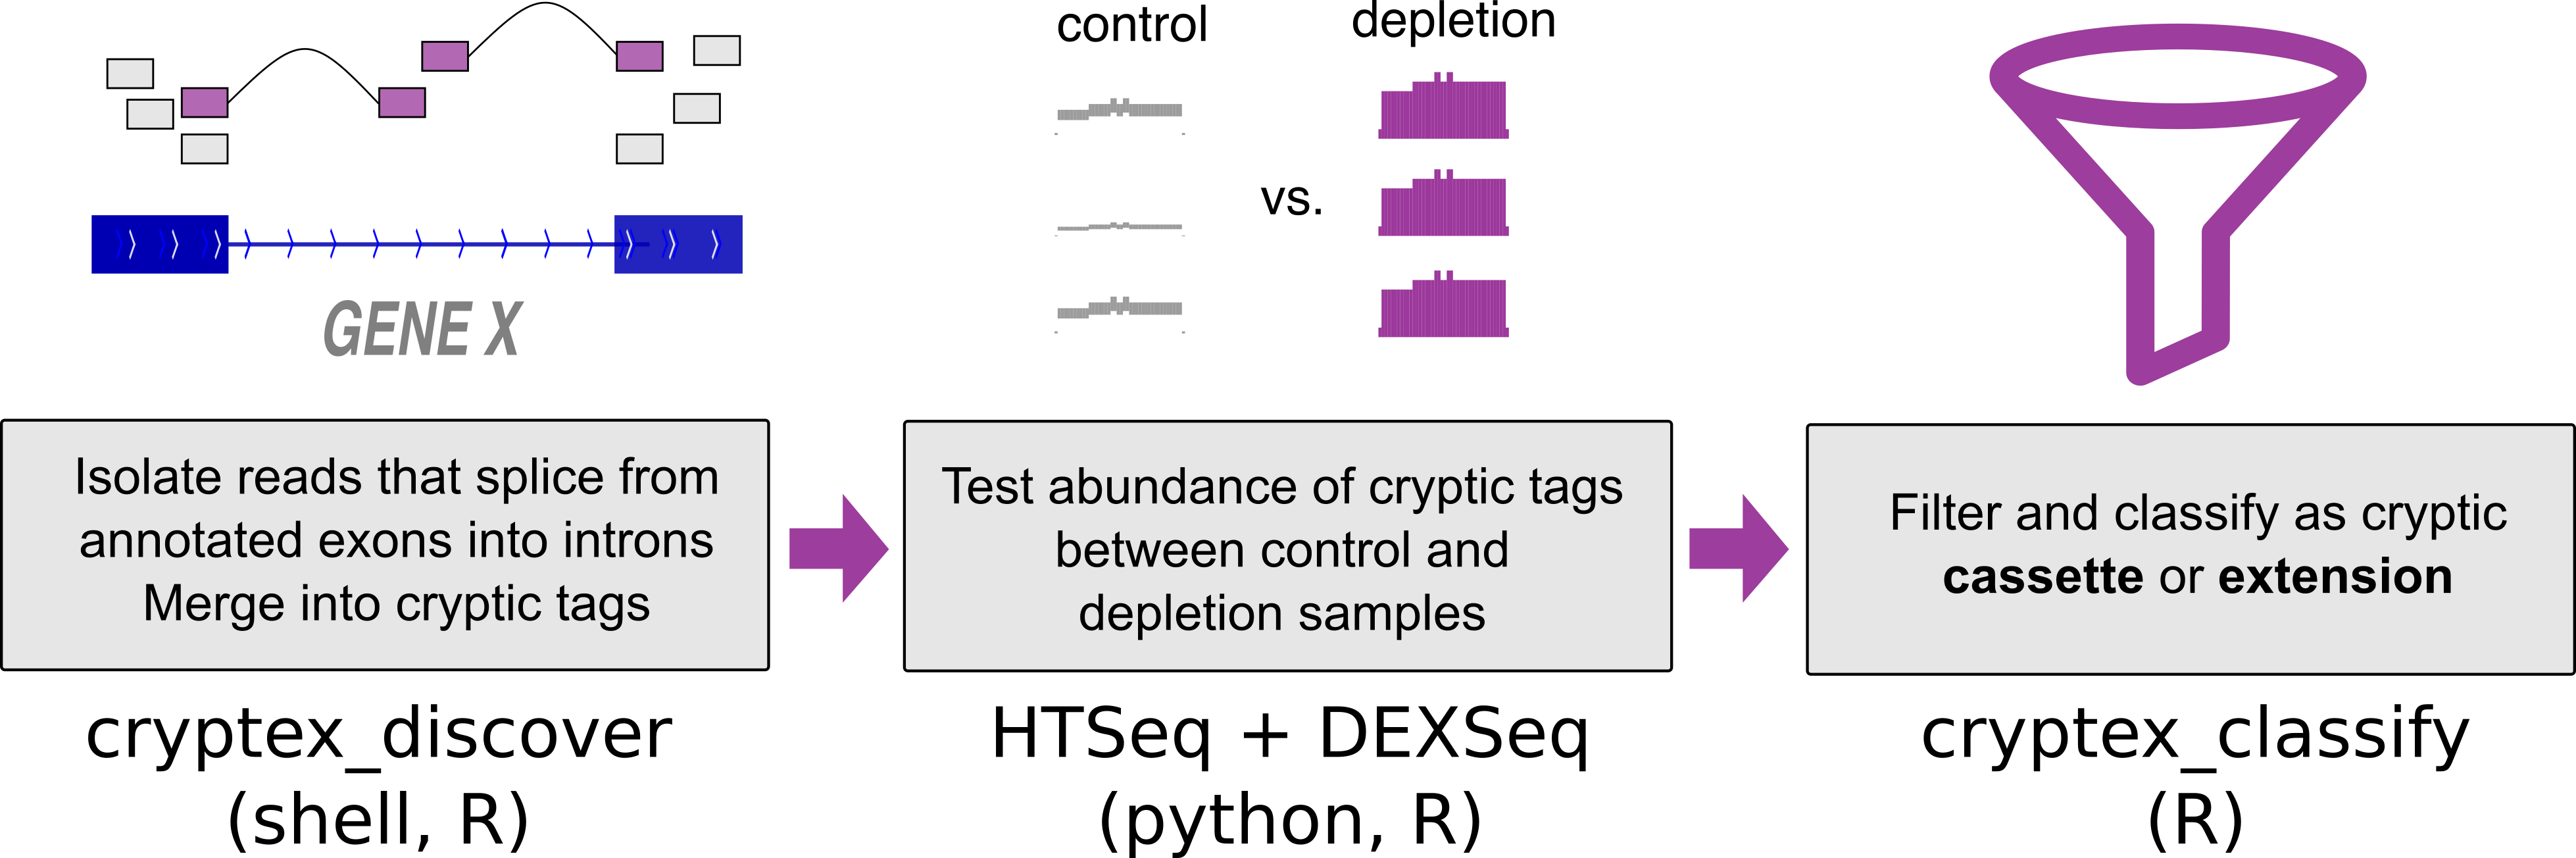
\includegraphics[width=14cm]{Figures/03_cryptic_exons/cryptex_pipeline.png}
	\caption{\textbf{Schematic of the \textit{Cryptex} workflow}}
	\label{cryptic_workflow}
\end{figure}


RNA-seq is a constantly improving technology. As I wanted to analyse all TDP-43 depletion data created from 2010 onwards, the use of modern RNA-seq analysis software, with its requirement for long reads and high depth paired-end stranded sequencing, was sadly out of the question. The cryptic splicing discovery pipeline (\textit{CryptEx}) I developed is designed to be used on any RNA-seq library, whether single or paired end, stranded or unstranded, total RNA or polyA-selected RNA. This flexibility inevitably results in a large number of false positive hits which have to be aggressively filtered downstream. I am indebted to Yafang Li and colleagues whose paper on intron retention \citep{Li2015-en} was the inspiration for my repurposing of existing bioinformatic tools to mine published data for an overlooked RNA phenotype.
 
I wrote the code for \textit{CryptEx} in the Bash shell scripting language, making use of the \emph{SAMTools} (version 1.2) \citep{Li2009-hm} and \emph{BEDTools} (version 2.25.0) \citep{Quinlan2010-up} libraries of commands for manipulating read alignments and lists of genomic features respectively. Reads were counting using HTSeq \citep{Anders2015-wz}. The statistical testing for differential cryptic exon usage was carried out using the \textit{DEXSeq} package \citep{Anders2012} in the R statistical computing environment. I subsequently wrote all code for downstream processing and filtering of cryptic hits in the R language (version 3.1.1) due to the wealth of existing software packages for genomic analysis, data processing and visualisation. I made extensive use of the \emph{Biostrings, data.table, DEXSeq, dplyr, GenomicRanges, ggplot2, gridExtra, optparse, plyr, stringr,} and \emph{tidyr} packages. The code for reproducing the results of this chapter is available in a GitHub repository \url{www.github.com/jackhump/CryptEx}.

In order to discover all possible splice junctions that travel into the intron, spliced reads were extracted from each aligned bam file using \emph{SAMTools}, discarding any secondary alignments. To extract only the spliced reads that overlap an annotated exon the lists of spliced reads were intersected in \emph{BEDTools} with a flattened list of exons, created using the \url{dexseq\_prepare\_annotation.py} Python script included with the \emph{DEXSeq} package \citep{Anders2012}. An inverse intersection was then performed with the same exon list to retain only the spliced reads which do not bridge two annotated exons. The intronic mapping sections of each read were split off from the rest and retained, thus keeping a set of aligned reads that splice to, but are not part of, an annotated exon. The results of this for each sample were merged together irrespective of condition. Split reads that were within 500bp of each other were merged into larger intervals, hereby referred to as tags. This ideally captures both the upstream and downstream splice junction to a central cryptic cassette exon.  To keep only the tags that are splicing within the gene body another intersection was performed with a list of introns. This was generated from the same flattened exon file by an R script written by Devon Ryan (\url{seqanswers.com/forums/showthread.php?t=42420}). The tags were then incorporated into the flattened list of exons, the GFF file. Each tag was given a unique identification number including a reference to the upstream annotated exon, allowing for comparisons of different datasets. The reads that overlap annotated exons and tags were counted using \textit{HTSeq} \citep{Anders2015-wz} on the default settings, ignoring reads marked as PCR duplicates. The read counts were used to calculate differential usage of each exon with respect to condition with \textit{DEXSeq}. 

All the cryptic tags with an adjusted P-value (false discovery rate) $<$ 5\% and a $|\log_{2}$(fold change)$| > 0.6$ were extracted from the \textit{DEXSeq} results table. The splice junctions from the alignment of each sample were used to work out the coordinates of the canonical junction that spans the intron within which the cryptic tag is or isn't spliced in control samples. Using splice junctions from the depletion condition samples, the upstream and downstream junctions that connect the adjacent annotated exons to the cryptic tag were re-discovered and quantified. Any cryptic example that did not have at least one upstream or downstream junction per sample or had fewer than ten canonical splice junctions was removed. These junctions were used to calculate per-condition mean Percent Spliced In (PSI) values which are a ratio of cryptic splicing over the sum of cryptic and canonical splicing \citep{Katz2010-ir}. As a number of cryptic splicing events are present at a low level in control samples, $\Delta$PSI values were created for both upstream and downstream splicing for each tag. This is the difference in PSI between the depletion samples and the control samples. Any cryptic tag that had either an upstream or downstream $\Delta$PSI $<$ 5\% was removed.




\subsection{iCLIP/eCLIP enrichment}
Crosslinking and immunoprecipitation is a method to identify the RNA targets of RNA-binding proteins \citep{Ule2003}. This involves UV crosslinking of RNA-protein interactions within a sample and immunoprecipitating the crosslinked RNA-protein complexes with an antibody against the RNA-binding protein of interest. Individual nucleotide resolution CLIP (iCLIP) is an extension of CLIP which allows for very precise spatial measurement of protein binding to RNA  \citep{Huppertz2014-ip}. An extension to iCLIP that allows for higher throughout and easier sample preparation is eCLIP \citep{Van_Nostrand2016-su}. Both methods create stranded RNA-sequencing libraries from the bound RNA. By comparing RNA populations between immunoprecipation with a specific and non-specific antibody, peaks of protein binding can be mapped to the genome with high confidence. I downloaded lists of iCLIP and eCLIP peaks (see Table 3.1) and used the UCSC LiftOver tool to convert the coordinates into the human build 38 and mouse build 10.
The coordinates of each cryptic tag were flanked by 100 base pairs on either side to capture binding around the putative splice sites. In order to compare the overlap between cryptic exons and RNA-protein binding peaks, two sets of null exons were created for comparison, which maintain the same length as their corresponding cryptic exon but sample either the intronic sequence outside of the flanked exon or that of the adjacent introns within the same gene if available. Overlaps between exons and iCLIP and eCLIP peaks were calculated using BedTools. The proportions of overlap between the cryptic exons and the two sets of null exons were compared using a proportion test with the null hypothesis that the proportion of exons overlapping an iCLIP or eCLIP peak would be the same.

\subsection{Motif enrichment analysis}
FASTA sequence was generated for the cryptic exons flanked by 100 nucleotides either side and submitted to the \emph{MEME} web tool \citep{Bailey2009-lw} under the default settings. The analysis was repeated using the \emph{HOMER} algorithm \citep{Heinz2010-ym} on RNA mode. Motifs were created using \emph{WebLogo} \citep{Crooks2004-yg}. Frequencies of the 16 possible dinucleotides were compared between flanked cryptic exon sequences with adjacent intron sequences from the same set of genes.

\subsection{Transposable element enrichment} 
Lists of transposable elements in human and mouse (hg38 and mm10 respectively) were previously generated by the \emph{RepeatMasker} tool \citep{Smit_AFA_Hubley_R_Green_P2015-ye} and were downloaded from UCSC. Overlap between different transposable elements and the cryptic exons was calculated in each orientation using \emph{BedTools}. 

\subsection{Conservation analysis}
\textit{PhyloP} compares the sequence alignments of multiple species to produce per base conservation scores \citep{Pollard2010-fj}. Average conservation score per cryptic tag was calculated using \emph{bigWigSummary} (UCSC) for both human and mouse data. The lists of splice junctions created by \emph{STAR} when aligning each sample were used to identify the coordinates of the exons adjacent to the cryptic exon. The randomly sampled intronic sequence from the cryptic-containing intron was used as a negative control.

\subsection{Protein prediction analysis}
Any cryptic exon which did not fall within the coding sequence of a transcript was omitted. Splice junctions were used to determine the upstream and downstream exons adjacent to each cryptic exon. These exons were matched to their corresponding annotated exon in the Ensembl transcript file for each species to work out the correct frame of translation. Nucleotide sequences for transcripts either including or excluding the cryptic tag were created. If the cryptic exon had been previously flagged as an extension then the entire continuous intronic sequence was inserted up to the remaining cryptic splice site. These transcripts were then translated \textit{in silico} and defined as premature termination codon (PTC)-containing if the inclusion transcript contained a stop codon and as a frameshift if the sequence of the downstream exon no longer matched. A null distribution of PTC-containing or frame shifted transcripts was created by shuffling the identity of the central exon 1000 times. 

\subsection{Splice junction scoring }
The strength of 5\'\ and 3\'\ splice sites was calculated for the human cryptic exons using \emph{maxEnt} \citep{Yeo2004-pz}. Higher scores indicate the increased log odds of a given splice site being a true splice site. The 5\'\ splice site is defined as the last 3 nucleotides of the upstream exon flanked by 6 intronic nucleotides, of which the first two are invariably GU. The 3\'\ splice site is defined as the last 20 intronic nucleotides of which the final two are invariably AG, flanked by the first 3 nucleotides of the downstream exon. The splice sites of annotated exons were used as a positive control. Randomly generated sequence with invariant AG or GT was used as a negative control. Paired t-tests were carried out to test the direction of change between the cryptic and annotated splice sites for each class of cryptic exon.


\section{Results}
\subsection{Depletion of TDP-43 but not FUS results in cryptic exons}
I analyzed publicly available TDP-43 depletion RNA-Seq datasets (three human, three murine, datasets 1-6 in Table 3.2), FUS depletion RNA-Seq datasets (1 human, 1 murine, datasets 7-8 in Table 3.2) and as a positive control a human hnRNP C depletion dataset for which cryptic exons have previously been reported (dataset 9 in Table 3.2).  While these datasets differ in library preparation method, read depth and length, and protein depletion method (Table 2), the FUS datasets match the TDP-43 datasets in cell type. 
Significant cryptic exons discovered by \textit{Cryptex} were classifed into three categories: (i) cassette-like, where novel 3\'\ and 5\'\ splice sites are recognised, which forms a completely new exon; (ii) 5\'\ extension, where a novel 3\'\ splice site is recognised and an existing exon is extended upstream of its annotated start and (iii) 3\'\ extension, where a novel 5\'\ splice site is recognised and an exon is extended downstream of its annotated end (Figure 3.1A). Note that \textit{Cryptex} does not consider fully retained introns, but other methods have been designed for this purpose \citep{Li2015-en,Bai2015-aq}.

Figure 3.1A lists the counts of both pre-classification cryptic regions (``unfiltered output'') and the post-classification cryptic exons. Comparing the two human ENCODE K562 cell line TDP-43 depletion datasets (3-4), the poly-A selected mRNA-Seq dataset yielded far more splicing events than the total RNA dataset, presumably due to polyA selection leading to a higher coverage of mature spliced mRNA species. In total 95 human cryptic exons were discovered and classified, with the majority only detected in the mRNA-seq dataset. 11 cryptic splicing events were shared between datasets 3 and 4 (Figure 3.1C). Of the 26 human cryptic exons reported by Ling, 12 were detected in at least one of the two datasets 3 and 4. 

Both mouse datasets differ in both cell type (adult striatum in dataset 5 vs embryonic stem (ES) cell in dataset 6) and read depth (35-60M in dataset 5 vs 2-10M in dataset 6). 52  cryptic exons were identified in total, with 46 detected in the adult striatum and 15 in ES cells, with 6 exons observed in both. Of the 46 cryptic splicing events identified in murine samples by Ling et al, 13 were detected in at least one of datasets 5 and 6. Side by side visual inspection suggests that differences in library preparation and read depth are behind the low the concordance rates in both human and mouse, as cryptic exons detected in the higher depth dataset (K562 mRNA and mouse adult brain) can be observed by eye in the lower depth dataset (K562 total RNA and mouse ES cell). These exons currently fail to be detected by the \emph{CryptEx} algorithm.

No cryptic splicing events were shared between human and mouse as previously reported \citep{Ling2015}. Note that to report overlap with Ling and colleagues (datasets 1 and 2), the raw data was unsuitable for the cryptic exon discovery pipeline due to a lack of biological replicate samples. Instead the sequence data was aligned and the splice junctions generated by the aligner were used to classify previously reported cryptic exons.

In contrast, while a large number of novel splicing events were observed in the FUS depletion datasets, our algorithm only classified 3 in mouse and 1 in human as cryptic exons. FUS depletion was not observed to produce any cassette-like cryptic exons in either species. Appendix Tables 2 and 3 list the coordinates of each cryptic exon along with the results of each analysis.

\begin{table}[h!]
	\caption{\textbf{All RNA-sequencing data used in this study}}
	 ES: embryonic stem cell. K562: human leukaemia cell line. siRNA: small interfering RNA. shRNA: short hairpin RNA. ASO: antisense oligonucleotide. PE: paired end sequencing. SE: single end sequencing. For single end sequencing, depth is measured in millions of mapped reads whereas paired end sequencing depth is measured in millions of mapped fragments.
	\label{table:cryptic_data}
	\centering
		\begin{small}
			\begin{tabular}{l|lllp{1.5cm}llll}
				& Species & Cell & Protein & Depletion method & Library & Read type & Depth & Citation\\
				\hline
				1 & Human & HeLa & TDP-43 & siRNA & mRNA & 100bp PE & 97-116M & Ling, 2015\\
				2 & Mouse & ES & TDP-43 & deletion & mRNA & 100bp PE & 70-75M & Ling, 2015\\
				3 & Human & K562 & TDP-43 & shRNA & RNA & 100bp PE & 55-62M & ENCODE\\
				4 & Human & K562 & TDP-43 & shRNA & mRNA & 100bp PE & 25-29M & ENCODE\\
				5 & Mouse & Brain & TDP-43 & ASO & mRNA & 75bp SE & 35-60M & Polymenidou, 2011\\
				6 & Mouse & ES & TDP-43 & deletion & mRNA & 40bp SE & 2-11M & Chiang, 2010\\
				7 & Human & K562 & FUS & shRNA & mRNA & 100bp SE & 12-21M & ENCODE\\
				8 & Mouse & Brain & FUS & ASO & mRNA & 72bp SE & 20-60M & Lagier-Tourenne, 2012\\
				9 & Human & HeLa & hnRNP C & siRNA & mRNA & 72bp SE & 26-28M & Zarnack, 2013\\
			\end{tabular}
		\end{small}
\end{table}


\begin{figure}[h!]
	\centering
  	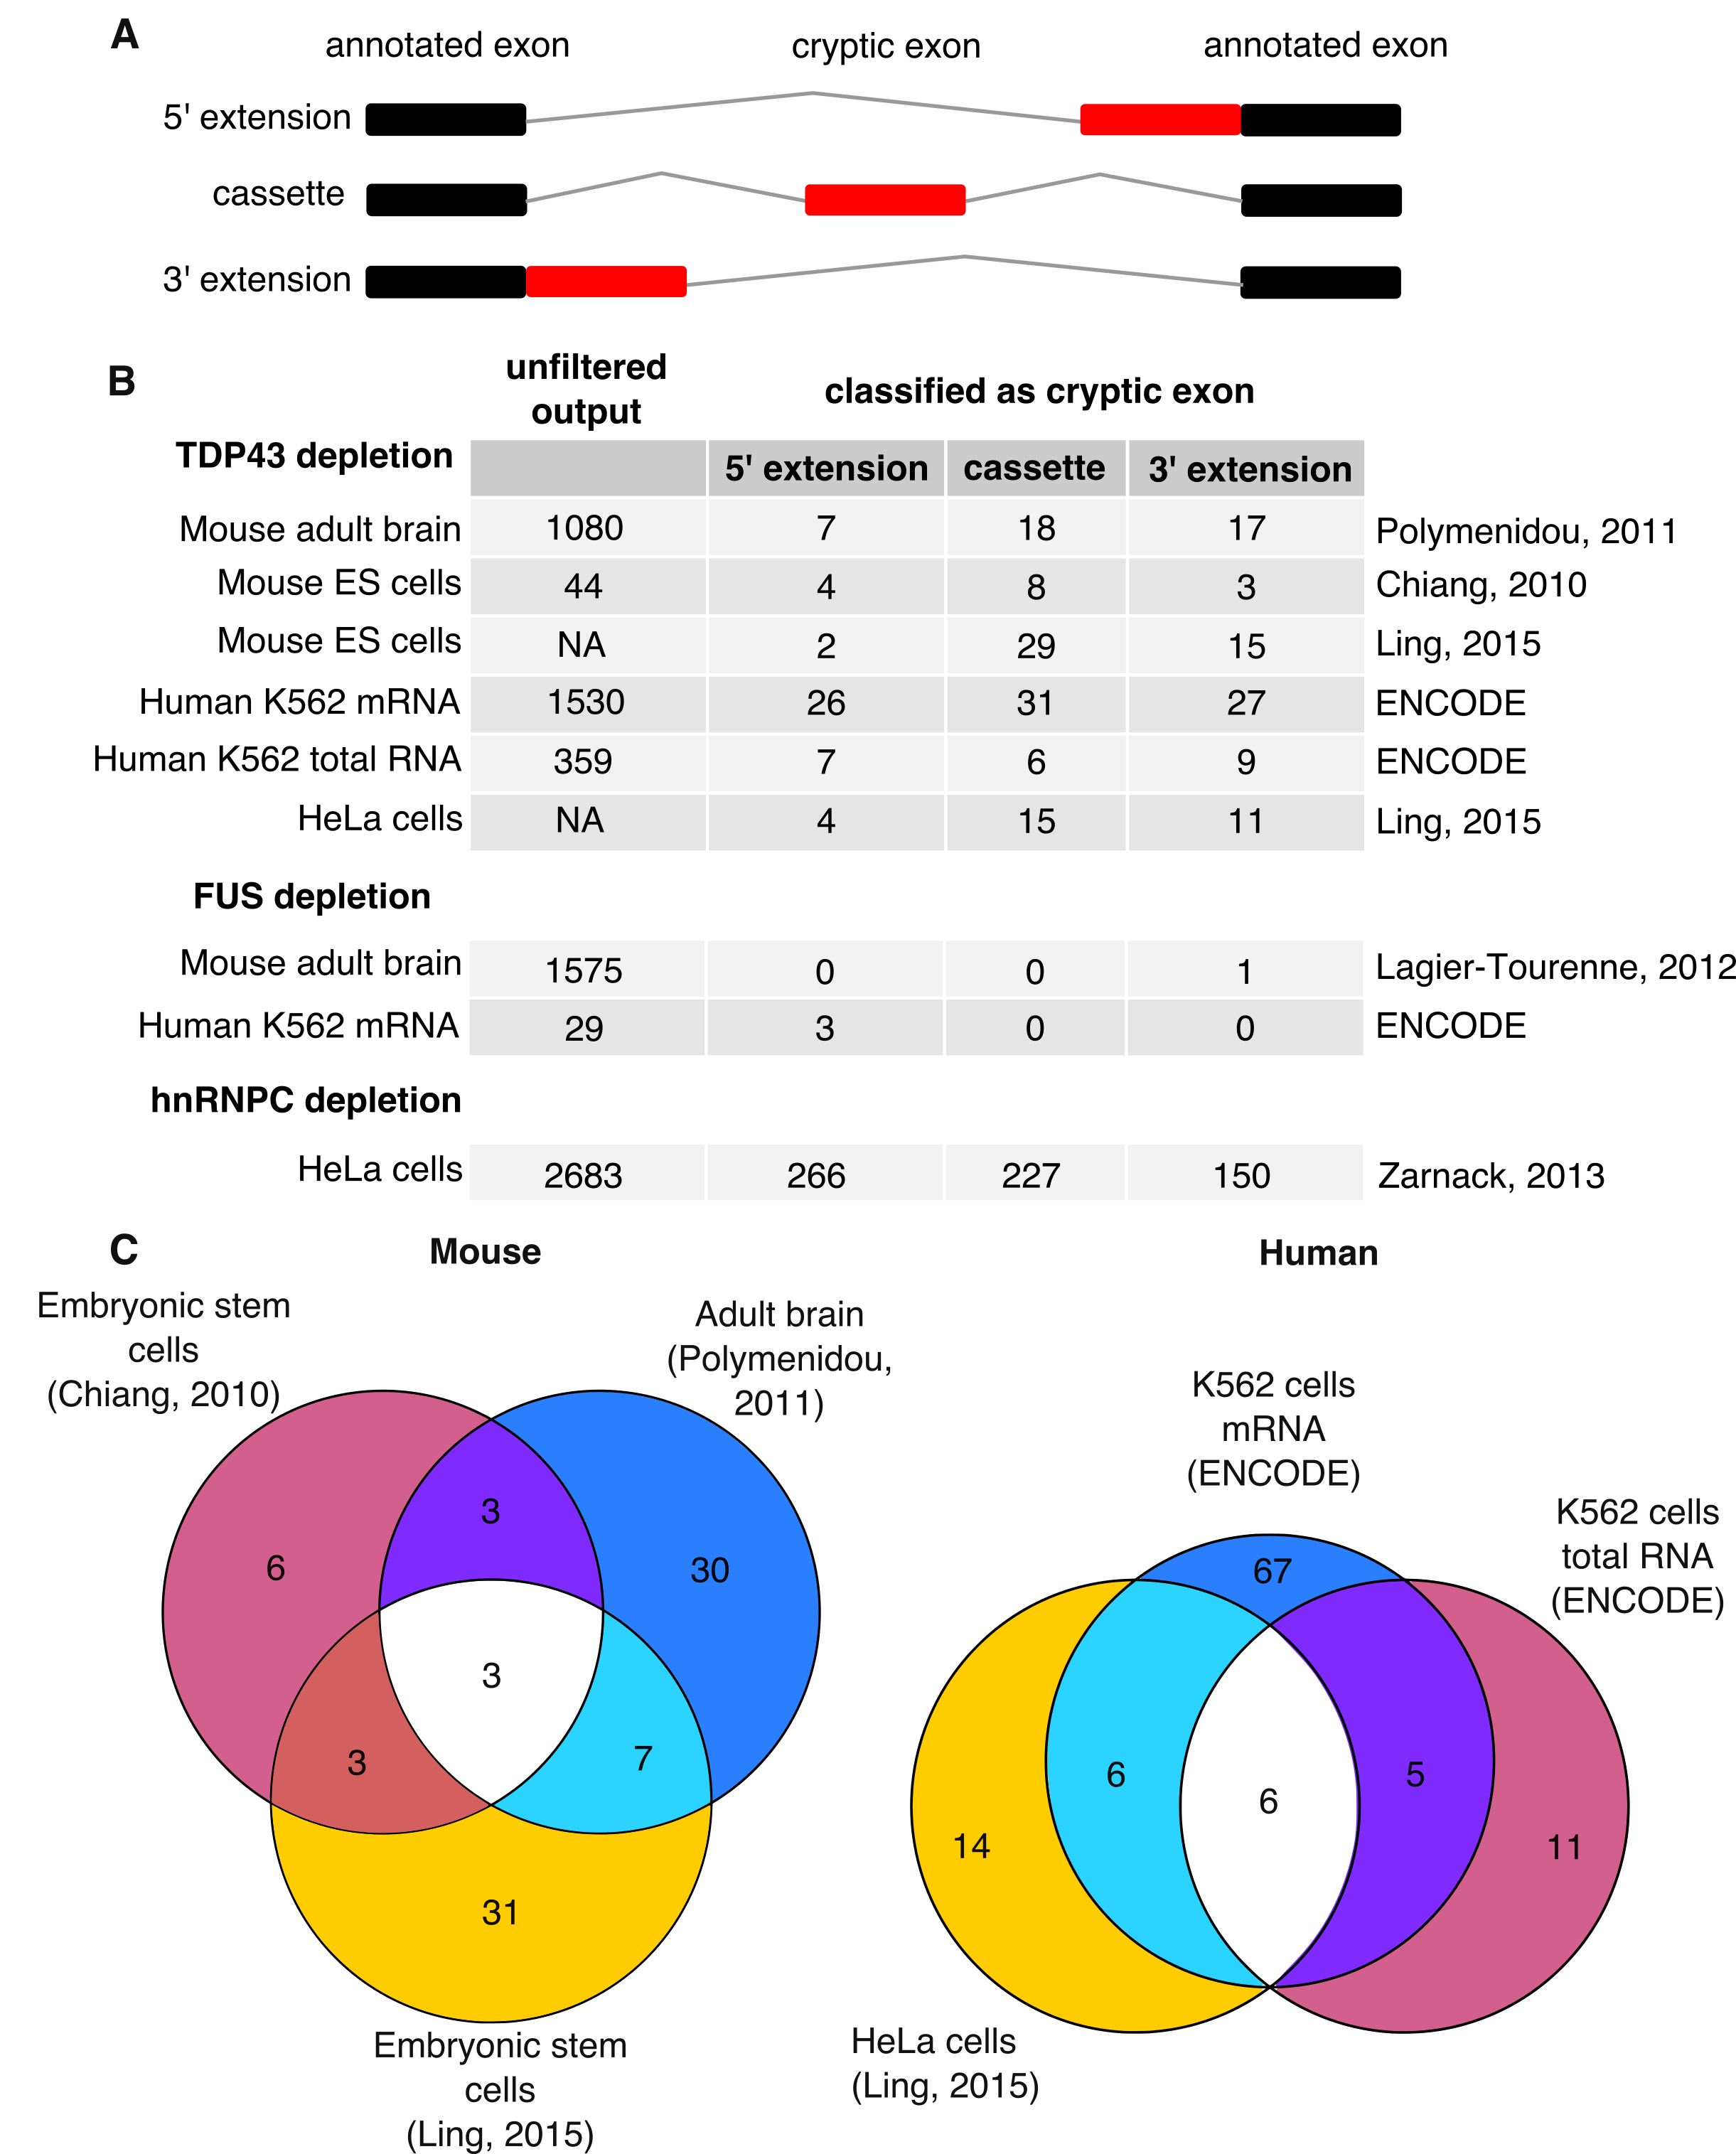
\includegraphics[width=\textwidth]{Figures/03_cryptic_exons/Figure_1_venn_inkscape.png}
	\caption{\textbf{Cryptic splicing discovered by the \emph{CryptEx} pipeline}}
		A) Schematic of the three classes of cryptic exon. Black boxes represent annotated exons and red boxes represent a cryptic exon. Grey lines represent the spliced intron. B) Tally of the three classes of cryptic exon discovered by the Cryptex pipeline across the nine datasets. ``Unfiltered output'' refers to the number of differentially used cryptic splicing events at a false discovery rate (FDR) $<$ 5\% before undergoing cryptic exon classification. Counts from Ling et al's data are taken from the paper itself. C) Venn diagrams showing the overlap between the six TDP-43 depletion datasets.
	\label{fig:cryptic_venn}
\end{figure}


\subsection{Cryptic exons are bound by TDP-43}
TDP-43 linked cryptic exons were grouped into unions of all cassette-like exons and extension events discovered in human and mouse, totalling 95 human and 52 murine cryptic exons. I then explored whether TDP-43 binding could explain the observed splicing changes in RNA-Seq data, as observed by Ling and colleagues. I took two complementary approaches: (i) searching for enriched motifs in the RNA sequence including and surrounding the cryptic exons and (ii) correlating the positions of cryptic exons with TDP-43 protein-RNA interaction data.

TDP-43 can repress or enhance the inclusion of a given exon by either binding within or adjacent to the exonic sequence \citep{Tollervey2011}. Hence, for our motif search, I flanked cryptic exon sequences by 100 nucleotides on either side. UG-rich motifs were found to be enriched in both mouse and human cryptic exons using two different algorithms: \emph{MEME} (Fig 3.2A) and \emph{HOMER} (appendix 1). Of the 52 mouse cryptic exons, 29 had a run of UG up to 40 nucleotides in length. Similarly, human cryptic exons were enriched in a UG motif but not in a continuous manner. By comparing  the frequencies of  16 possible dinucleotides between the flanked cryptic exon sequence and the sequence of the adjacent intron either up or downstream of the cryptic-containing intron it was possible to resolve the enrichment of UG dinucleotides (Fig 3.2D). UG and GU were enriched in flanked cryptic exon sequence in both human (fold change GU = 1.53; UG = 1.48; $P < 10^{-50}$; proportion test) and mouse (fold change GU = 2.14; UG = 1.85; $P < 10^{-50}$; proportion test). 
If TDP-43 binding was uniform throughout an intron or gene then one would expect to see similar proportions of overlap in each. However, both species show an enrichment in TDP-43 binding peaks specific to the cryptic exons in every iCLIP dataset used, with as much as 25\% of human cryptic exons and 50\% of mouse cryptic exons overlapping at least one iCLIP peak each (both species: $P < 10^{-16}$, proportion test). 

\begin{figure}[h!]
	\centering
	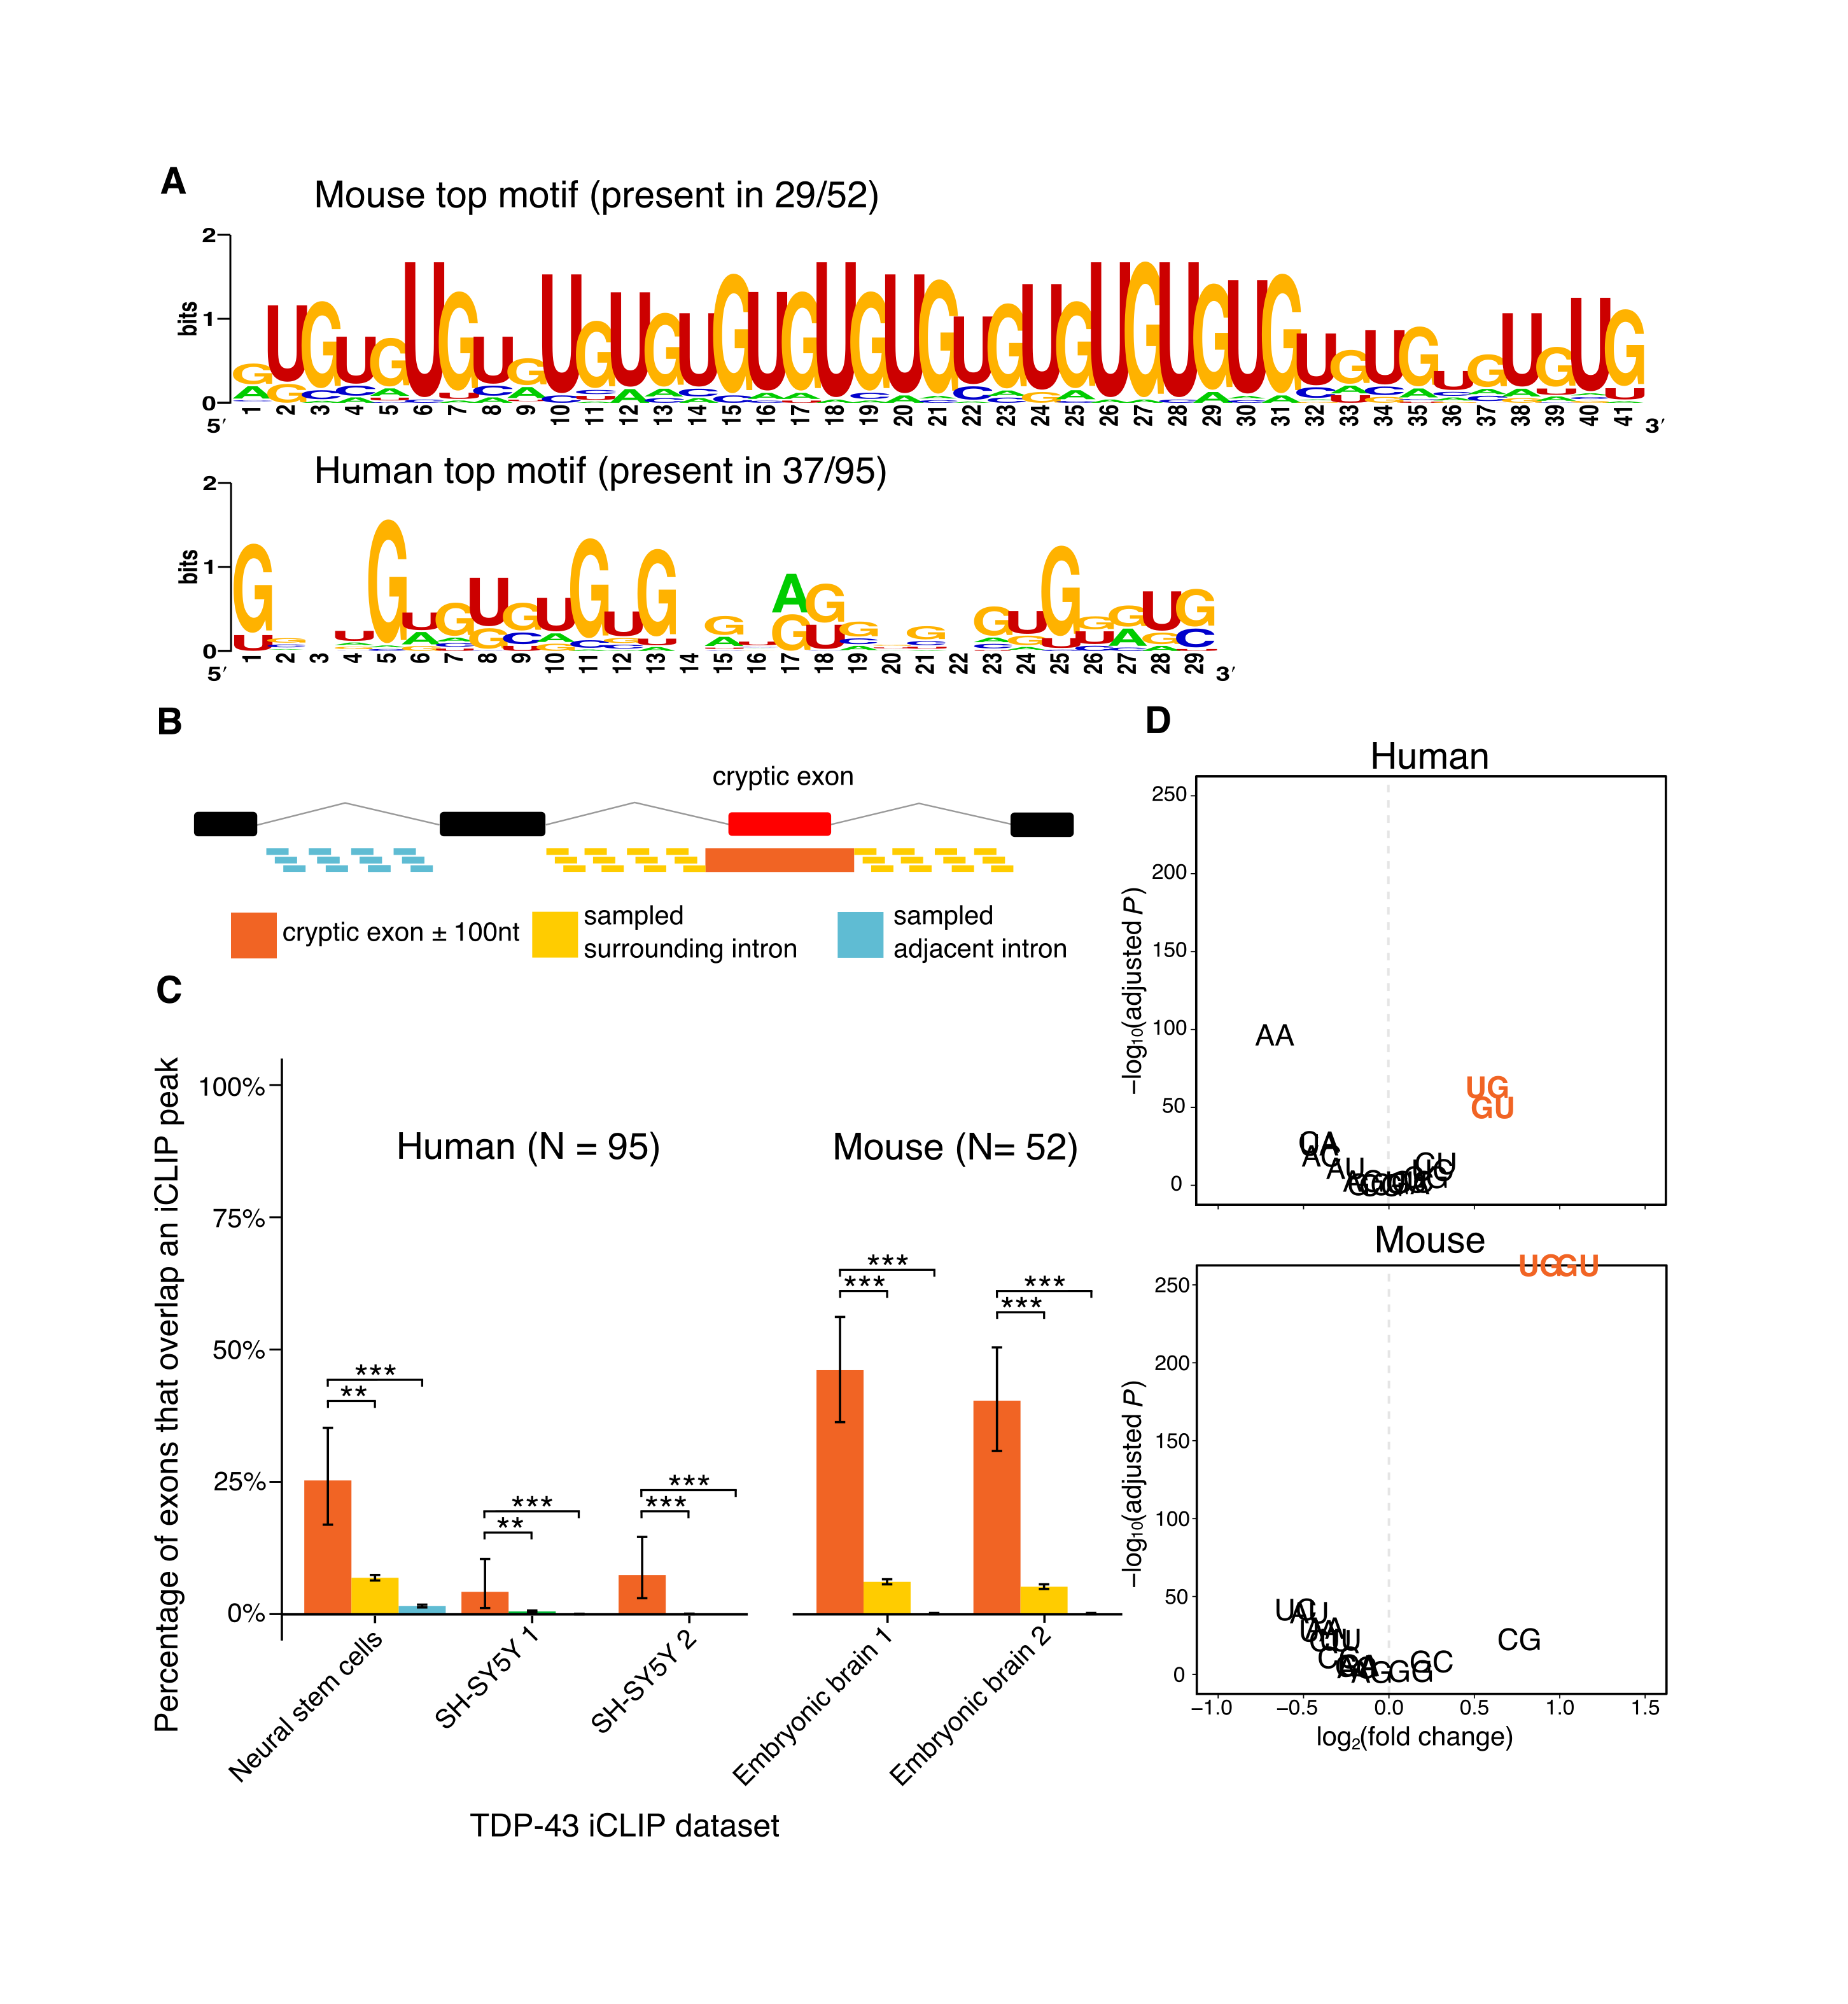
\includegraphics[width=\textwidth]{Figures/03_cryptic_exons/Figure_2_motif_iCLIP.png} 
	\caption{\textbf{Evidence of TDP-43 binding cryptic exons}}
		A) Results of \emph{MEME} motif search. Only the motif with the greatest enrichment compared to background sequence is presented. B) Schematic of iCLIP peak enrichment test. For illustration a cassette-like cryptic exon (green box) is shown between two annotated exons (black boxes) separated by intronic sequence (black lines). The proportion of the group of cryptic exons flanked either side by 100 nucleotides (orange) that overlap at least one iCLIP peak is compared to the proportion of overlaps in a group of length matched sequences from either the surrounding intron (yellow) or an adjacent intron (blue) each randomly sampled 100 times per gene. C) iCLIP peak overlap enrichment for the 95 human cryptic exons found in either K562 cell TDP-43 depletion dataset and the 52 cryptic exons found in either mouse TDP-43 depletion dataset. D) Dinucleotide enrichment in the flanked cryptic exons compared to adjacent introns. Error bars denote 95\% confidence intervals of the binomial distribution. $^* P < 0.05 $, $^{**} P < 0.001$, $^{***} P < 10^{-16}$ . All P-values adjusted for multiple testing by Bonferroni method.
	\label{fig:cryptic_motifs}
\end{figure}


\subsection{Cryptic exon recognition is unrelated to the binding of transposable elements by TDP-43}
TDP-43 has been demonstrated to bind antisense Alu elements, which are the source of cryptic exons repressed by hnRNP C \citep{Kelley2014-sr,Zarnack2013-nv}. I therefore investigated whether TDP-43 induced cryptic exons preferentially overlap specific families of transposable elements and/or class of repetitive sequences. Transposable and repeat elements annotations were obtained using the \emph{RepeatMasker} software, and these features were split by family and orientation. Although Alu elements are a subfamily within the primate SINE element family, I included them separately given the prior hnRNP C result.
Control regions were obtained as before. Figure 3.3 shows only modest enrichment patterns in the TDP-43 depletion datasets in the "simple repeat" family, owing to the aforementioned UG motifs. This contrasts with hnRNP C depletion, which shows a striking enrichment of antisense SINE elements of which all are of the Alu type ($P < 10^{-16}$, proportion test), a result consistent with previous analyses of dataset 9 \citep{Zarnack2013-nv}.

\begin{figure}[h!]
	\centering
	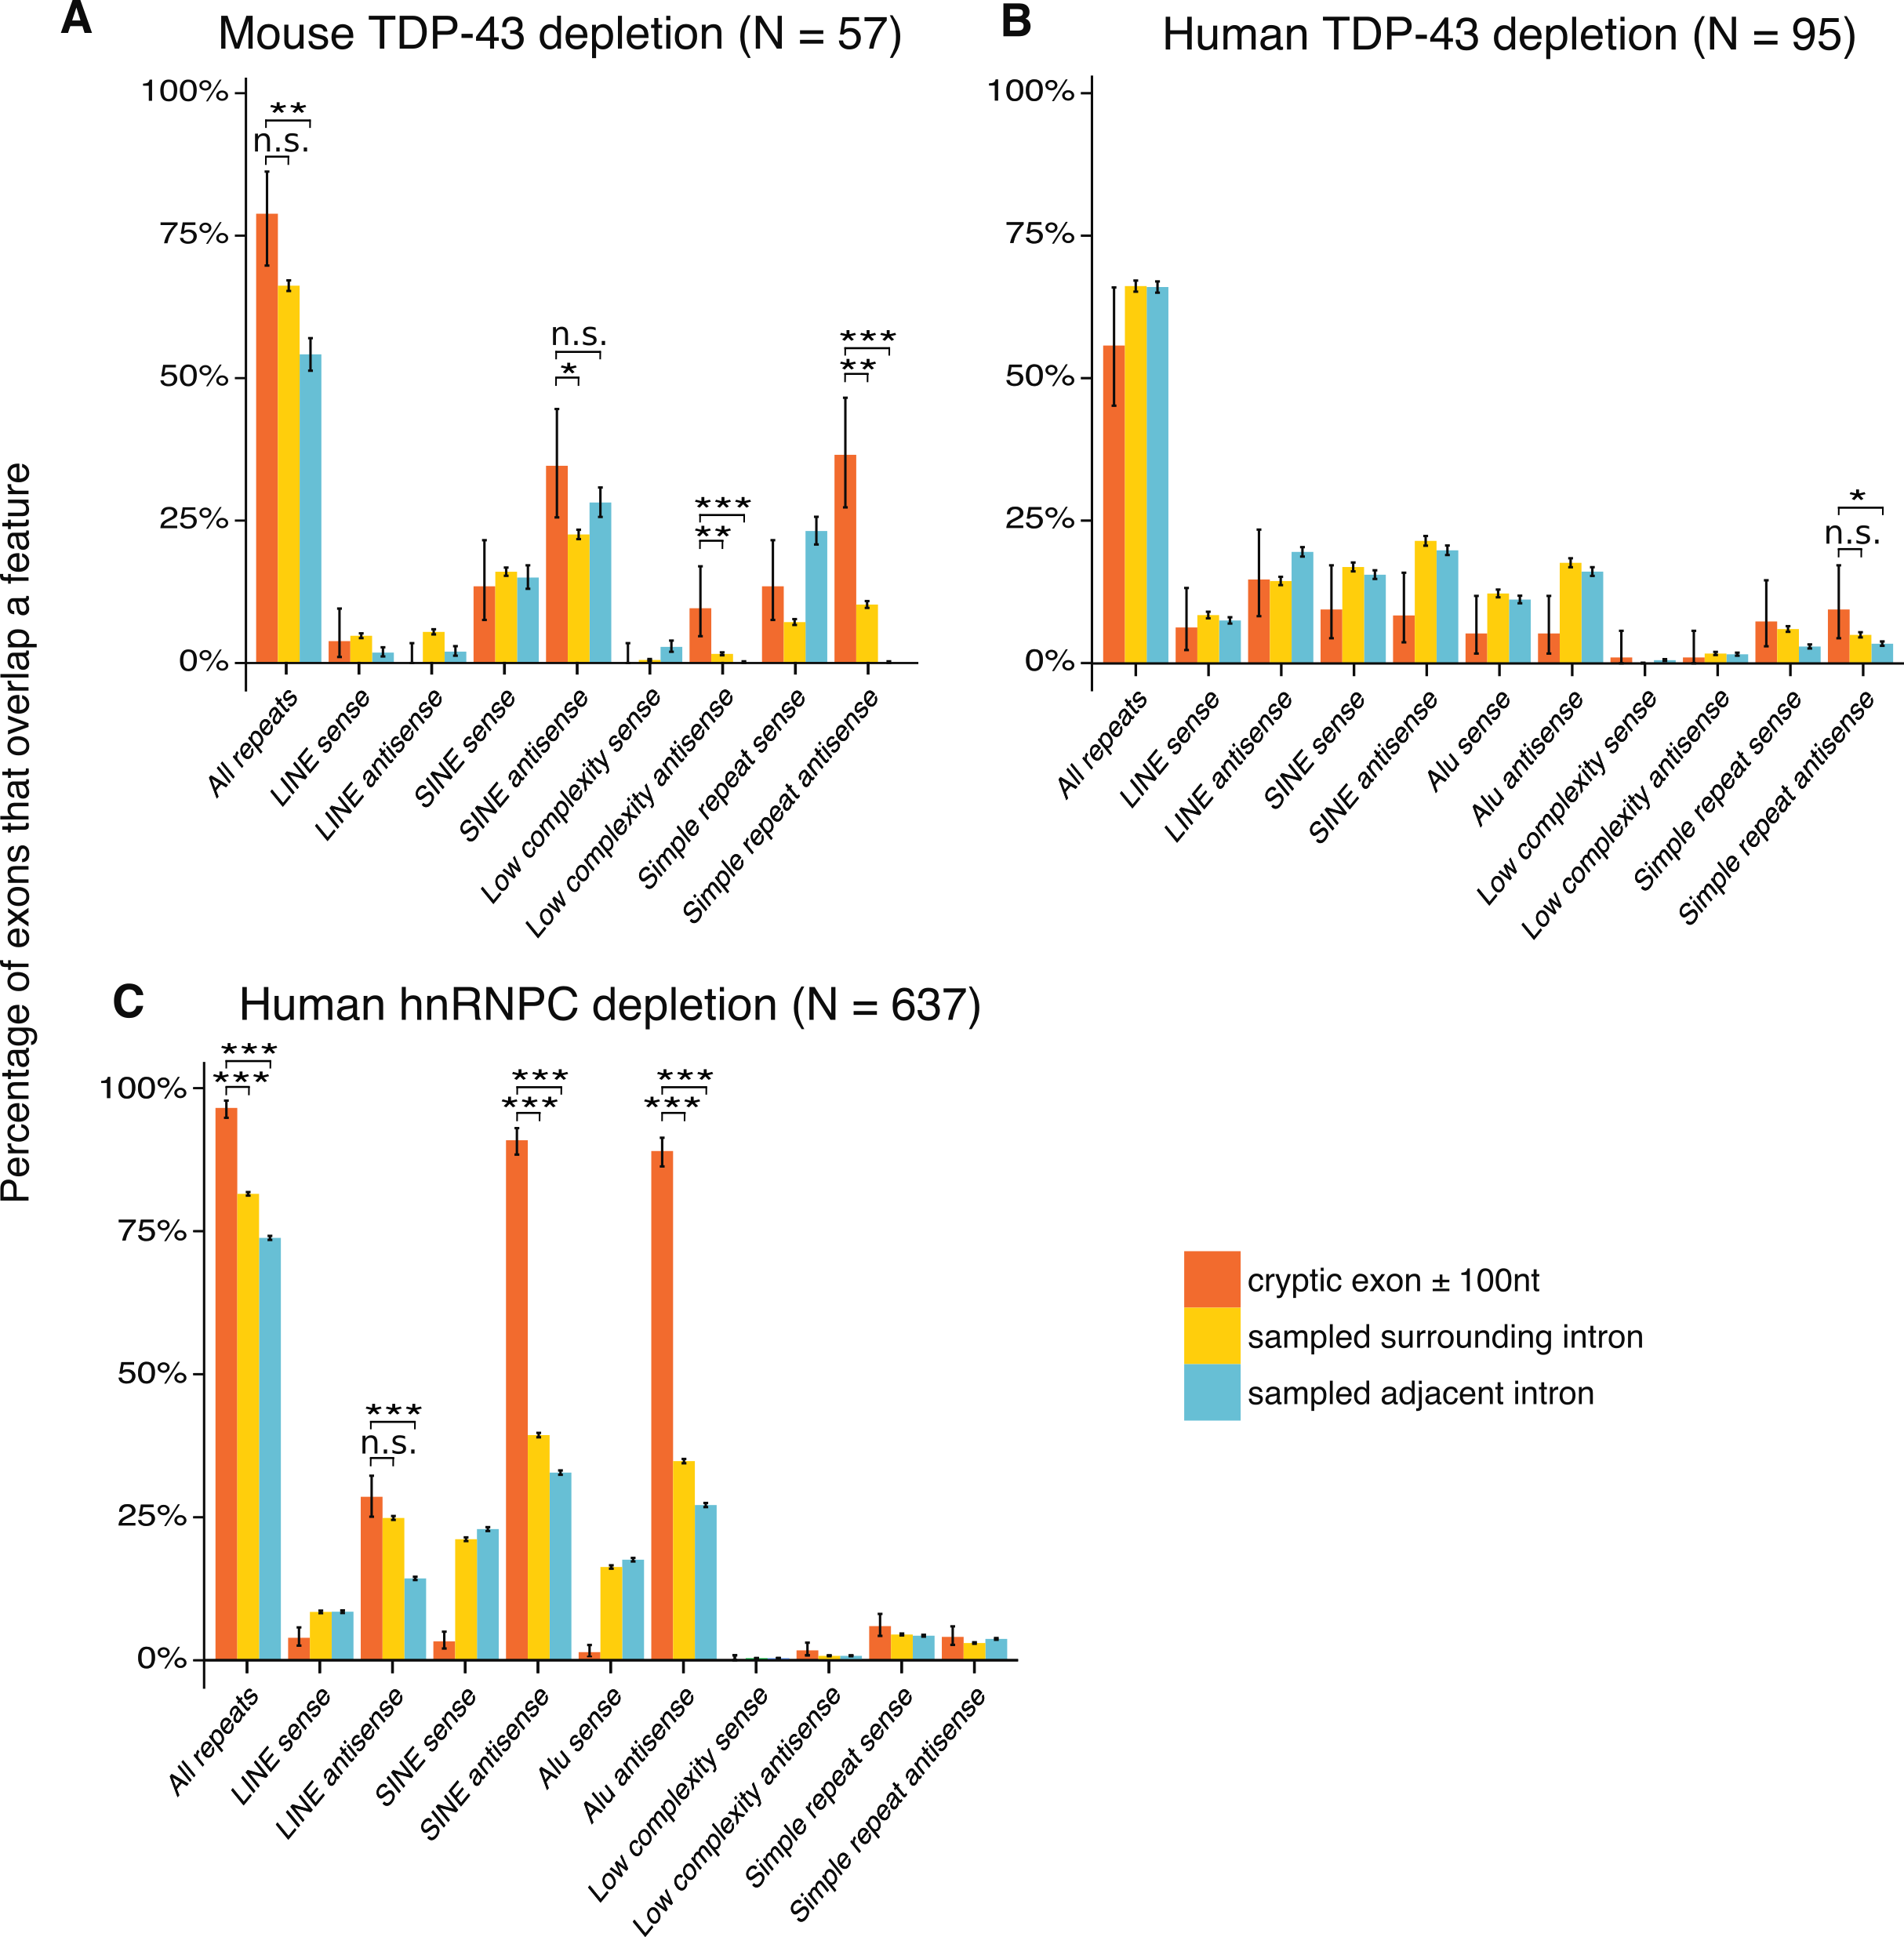
\includegraphics[width=\textwidth]{Figures/03_cryptic_exons/Figure_3_repeat_elements.png}
	\caption{\textbf{Cryptic exons in transposable elements}}
		Overlap between different families of repetitive element with lists of exons, separated by orientation. A) Mouse TDP-43 depletion. B) Human TDP-43 depletion. C) Human hnRNP C depletion. The proportion of the cryptic exons that contain a particular element are shown in orange. Length matched random samples from the surrounding intron (yellow) and adjacent introns (blue) are used as controls. LINE: Long Interspersed Nuclear Element; SINE: Short Interspersed Nuclear Element.  $^*: P < 0.05$, $^{**}: P < 0.001$, $^{***}: P < 10^{-16}$ . All P-values corrected for multiple testing with Bonferroni method.
	\label{fig:cryptic_repeats}
\end{figure}

\subsection{Cryptic exons are poorly conserved and generate premature stop codons}
I then quantified the extent of evolutionary conservation of cryptic exons using the multiple species alignment conservation scores generated by \textit{PhyloP}. I calculated mean conservation scores per exon for the cryptic exons and compared them to scores from both the annotated exons and randomly sampled intronic sequences from the same genes. No differences were observed between cryptic exons and matched intronic sequences (Figure 3.4A), and a much lower conservation level than adjacent annotated exons.

I also investigated the consequences of inclusion of cryptic exons on translation of the transcript. Potential outcomes for each gene are: (i) a functional transcript, (ii) a premature termination code (PTC) or (iii) a frameshift variant. I compared these estimates to random simulations where the identity of the included exon has been permuted 1000 times. The results were consistent with the null expectation, with around 66\% of cryptic exons leading to a frameshift due to length mismatches and less than 10\% of cryptic exons predicted to create functional transcripts (Figure 3.4B).

\begin{figure}[h!]
	\centering
	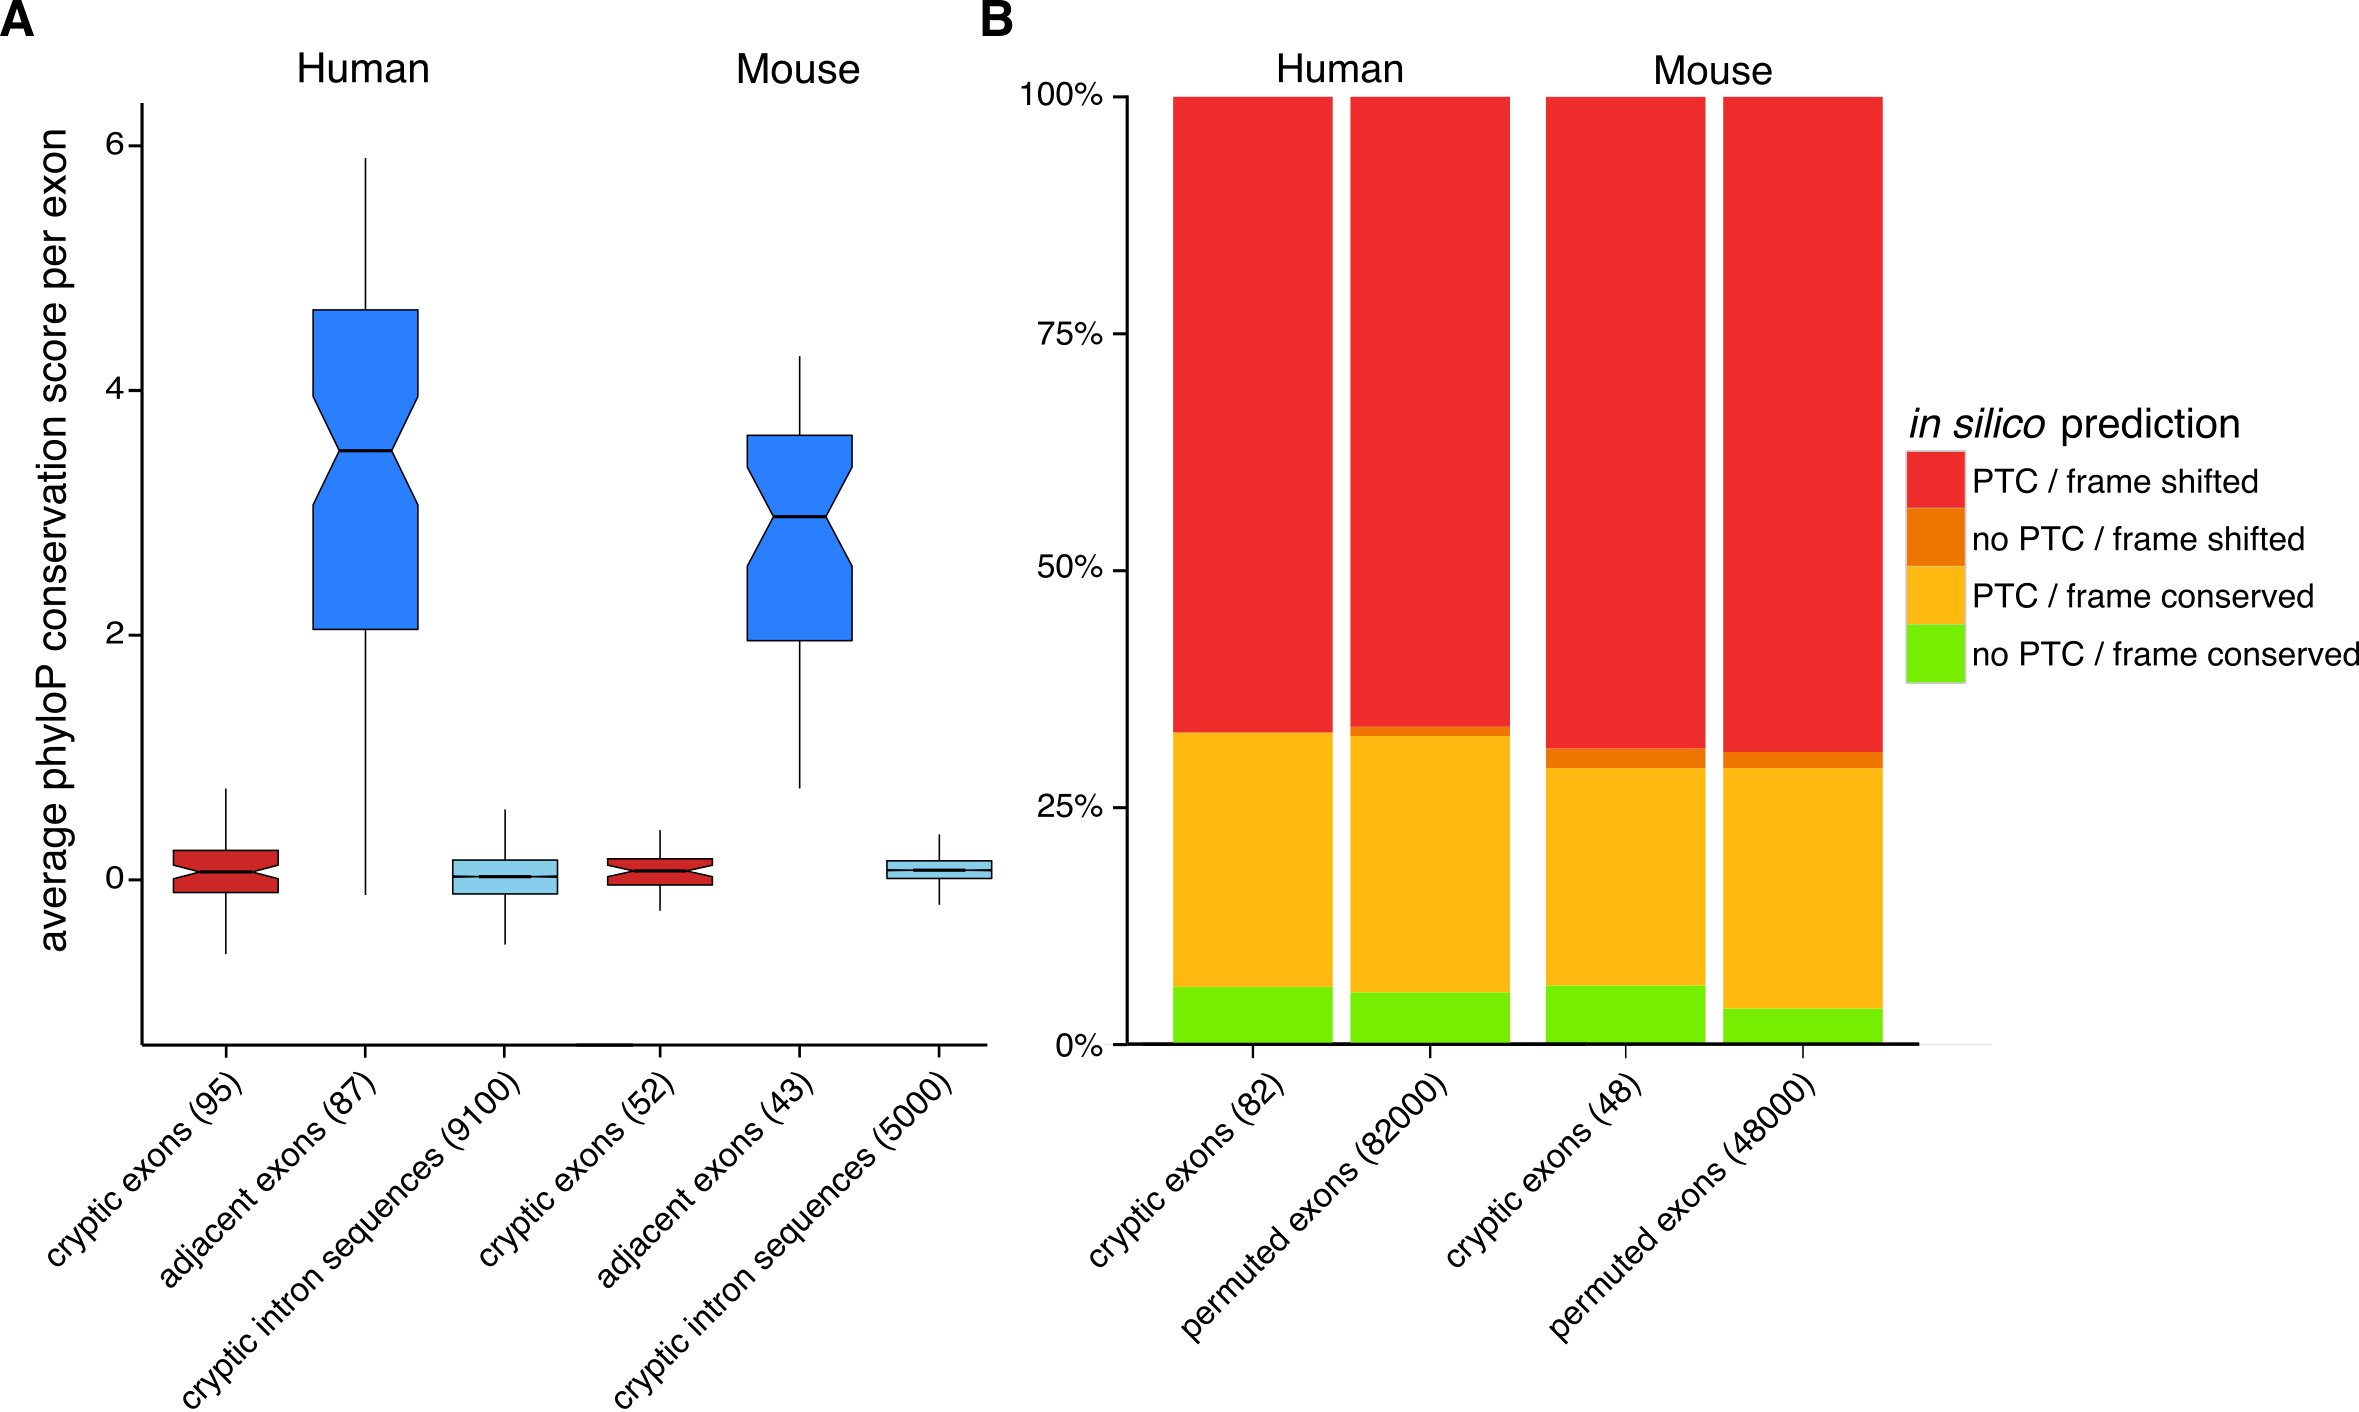
\includegraphics[width=\textwidth]{Figures/03_cryptic_exons/Figure_4_conservation_poison.png}
	\caption{\textbf{Conservation and premature termination codon analysis}} 
		A) Per exon average PhyloP conservation scores in cryptic exons, adjacent exons within the same set of genes (when available) and randomly sampled sequences from the cryptic containing intron. Box plots show first quartile, median and third quartile with the notches representing the 95\% confidence interval of the median. Whiskers represent the minimum and maximum values that fall within 1.5 times the interquartile range. B) The functional impact of cryptic exon inclusion on the host transcripts in human and mouse. Colours indicate the category of prediction and box size indicates the proportion of the total group of exons in each category. Categories from top to bottom: at least one premature termination codon (PTC) introduced and frame shifted (red); no PTCs introduced but frame shifted (orange); PTCs introduced but frame conserved (yellow); no PTCs introduced and frame conserved (green). For each species there is a corresponding set of null exons where the central exon has been permuted 1000 times.
	\label{fig:cryptic_conservation}
\end{figure}

\subsection{Cryptic exon containing genes are downregulated}
I then investigated, in datasets 3-6, whether genes containing cryptic exons showed a specific pattern of altered expression. I calculated the proportion of the cryptic exon containing genes in each dataset that were differentially expressed at a FDR of 10\%. This was then compared with the proportion of differential expression of all genes with an expression level at or greater than the lowest expressed cryptic exon found in that dataset. Figure 3.5A shows the number of differentially expressed genes in each dataset as a proportion of the total, separated by direction. In all four TDP-43 depletion datasets, the cryptic exon containing genes as a group are more likely to be significantly downregulated compared to the genome-wide proportion ($P < 0.001$, hypergeometric test).

Furthermore, I performed the same analysis for each dataset with the cryptic exon containing genes that were only found in the other dataset of the same species (Figure 3.5B). Surprisingly, in the mouse ES cell dataset 6 there was an enrichment of downregulated genes that contain cryptic exons only detectable in the mouse adult brain dataset 5 ($P < 0.001$, hypergeometric test). Visual inspection of these 10 introns in the mouse ES cell data suggests that 7 of them may harbour cryptic exons in the ES cell data that are currently undetectable by the \emph{CryptEx} algorithm.

\begin{figure}[h!]
	\centering
	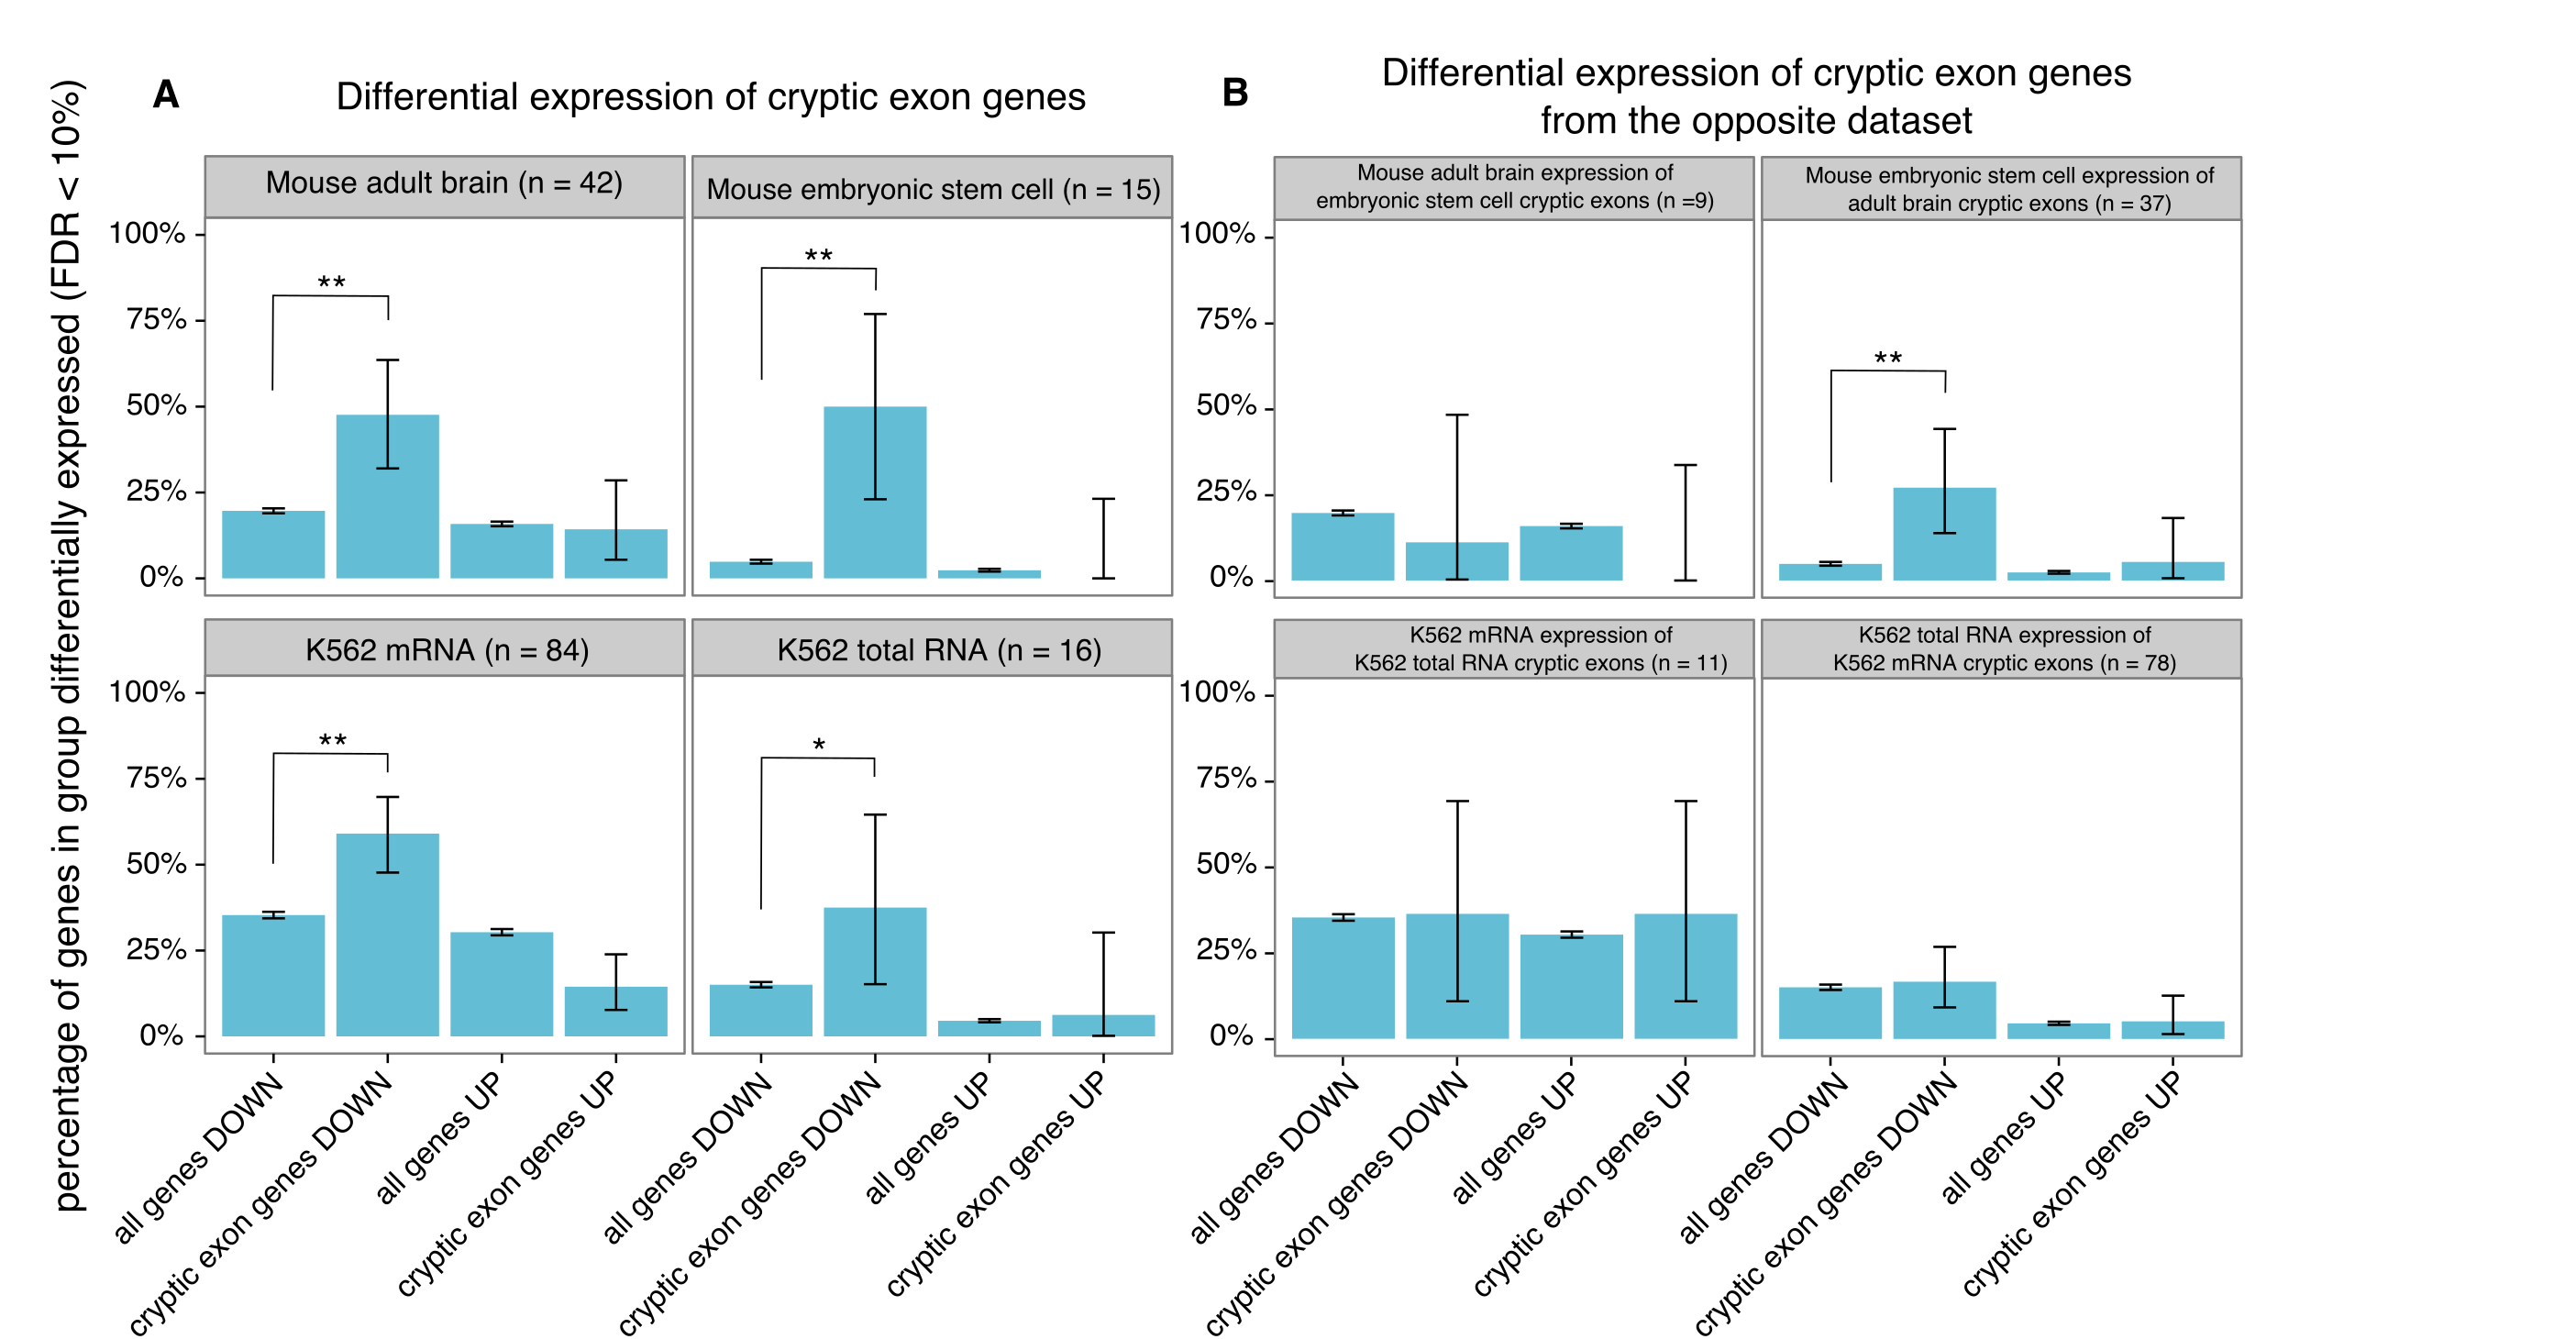
\includegraphics[width=\textwidth]{Figures/03_cryptic_exons/Figure_5_Gene_Expression.png}
	\caption{\textbf{Differential expression of cryptic exon genes}}
		A) Significantly differentially expressed genes between TDP-43 depletion and control samples (false discovery rate = 10\%) in datasets 3-6. Comparisons were made between all genes tested with an expression level at or greater than the lowest expressed cryptic exon (``all genes'') and the genes where cryptic exons were discovered (``cryptic exon genes'') with each group divided by direction of change. B) As above but for cryptic exon genes from the other dataset of the same species. Error bars show 95\% confidence intervals for each proportion. $^* : P < 0.05$, $^{**} : P < 0.001$. All P-values adjusted by Bonferroni correction.
	\label{fig:cryptic_expression}
\end{figure}

\subsection{Human cryptic exons are driven by the recognition of strong splice sites that are normally repressed}
Whereas cassette-like cryptic exons appear as separate exons distinct from their surrounding exons, extension events must rely on a switch from a canonical splice site to a newly accessible splice site. I hypothesised that these extension events result from competition between two splice sites upon TDP-43 depletion. This would require the sequence of and around the cryptic splice site to be similarly recognisable to the spliceosome. Using the \emph{MaxEnt} statistical model to score splice sites by comparing their DNA sequences with constitutive observed canonical sequences, I scored the 5\'\ and 3\'\ splice sites of our cryptic exons and compared them with the scores of the surrounding canonical splice sites. The model compares splice sites from annotated exons with decoy splice sites that retain the consensus AG/GT at the 3\'\ or 5\'\ splice site respectively. Therefore I also scored randomly generated sequences which retained the consensus AG/GT positions.  Figure 3.6 shows the scores for both the 3\'\ and 5\'\ splice sites for each class of human cryptic exons. Although the canonical splice sites were on average stronger than their corresponding cryptic splice site ($P < 0.05$, paired t-test), the majority had scores far greater than those from random sequence, suggesting that they are able function as real, albeit weaker, splice sites when TDP-43 is depleted.

\begin{figure}[h!]
	\centering
	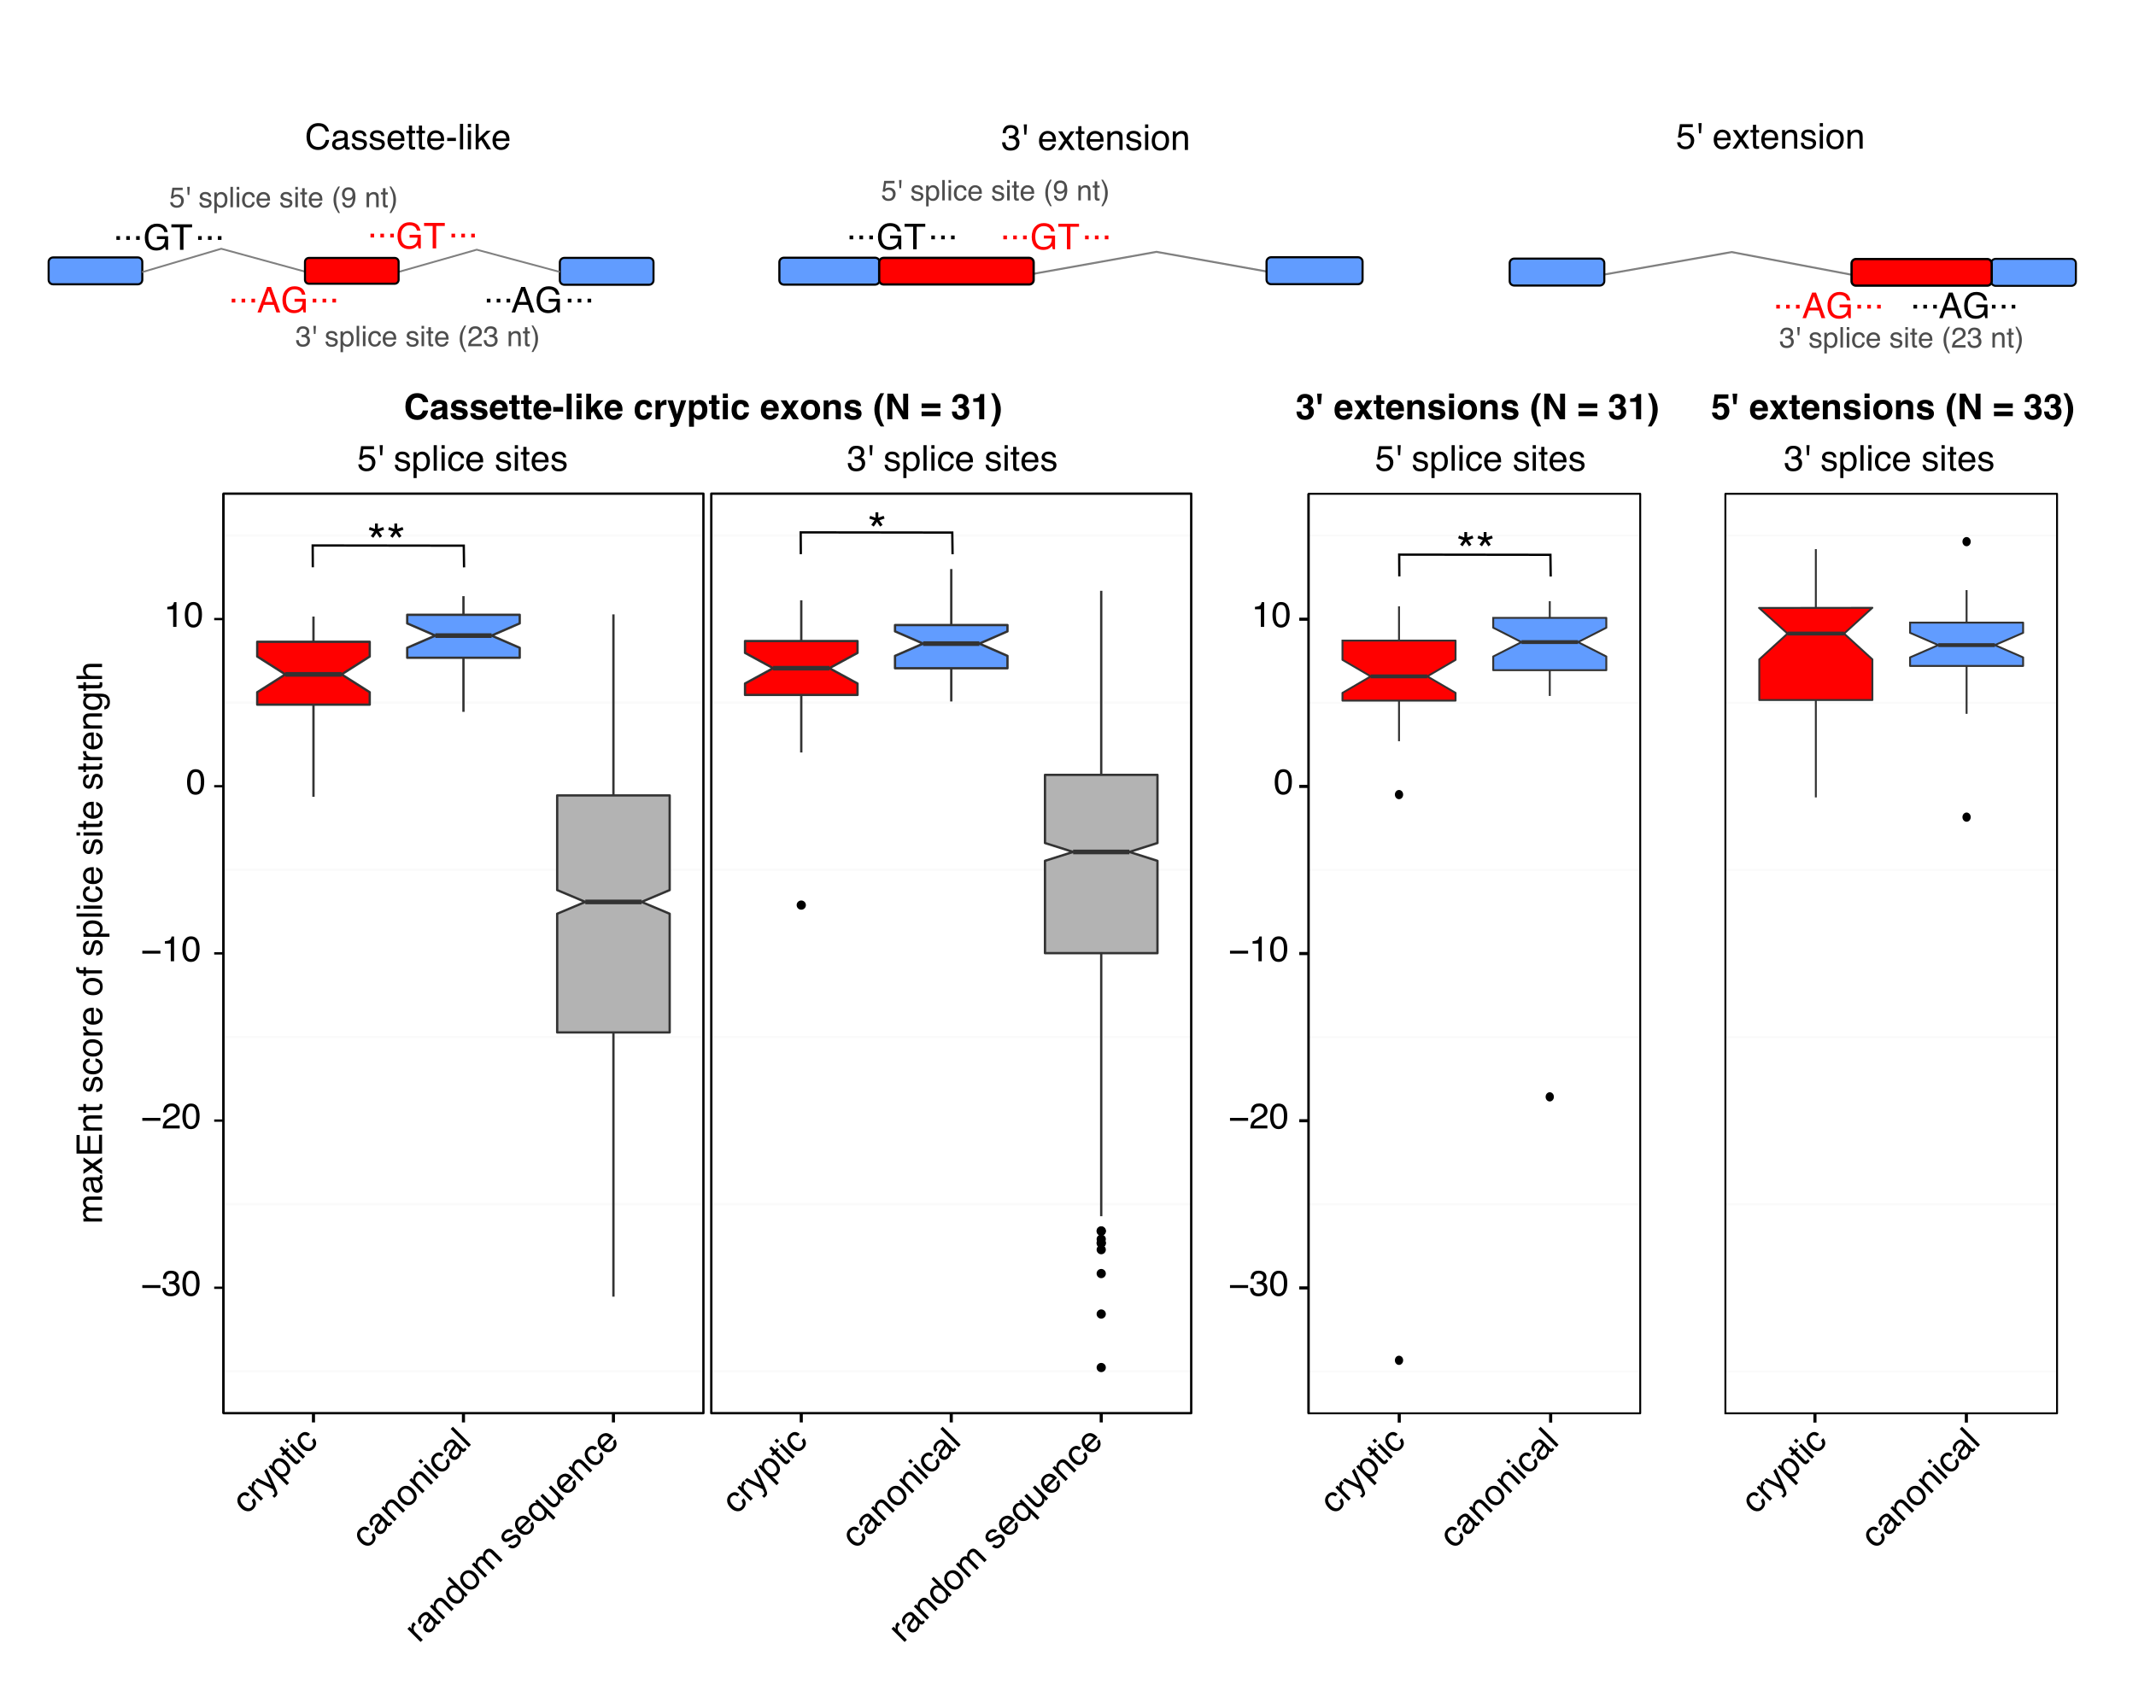
\includegraphics[width=\textwidth]{Figures/03_cryptic_exons/Figure_6_splice_site_scoring.png}
	\caption{\textbf{Scoring cryptic splice sites against canonical splice sites}}
		Cassette-like cryptic exons have 5\'\ and 3\'\ splice sites that are recognised by the spliceosome under TDP-43 depletion. 5\'\ and 3\'\ splice site scores are plotted separately. Cryptic splice sites are shown in red, canonical splice sites are shown in blue. Random sequences with AG or GT consensus are plotted in grey. Cryptic extensions are the result of a cryptic splice site competing with the canonical splice site. 5\'\ extensions result from cryptic 3\'\ splice sites whereas 3\'\ extensions result from cryptic 5\'\ splice sites. Box plots show first quartile, median and third quartile with the notches representing the 95\% confidence interval of the median. Whiskers represent the minimum and maximum values that fall within 1.5 times the interquartile range. Outliers are plotted as black dots. Cryptic splice sites are compared to canonical splice sites with paired t-tests. $^{*}: P < 0.05$, $^{**}: P < 0.001$.
	\label{fig:cryptic_scoring}
\end{figure}

\subsection{Cryptic exons are bound by other RNA binding proteins}
Proteomic studies have demonstrated that TDP-43 interacts with a number of RNA-binding proteins (RBPs), including multiple members of the heterologously expressed ribonucleoprotein (hnRNP) family and other splicing factors \citep{Blokhuis2016-hw,Ling2010-sr,Freibaum2010-hw}. The splicing of specific annotated exons has been shown to depend on the interaction of TDP-43 with multiple splicing factors \citep{Mohagheghi2016-zf}.  I hypothesised that some cryptic exons may be included indirectly through a loss of interactions with different RBPs. Van Nostrand and colleagues have performed eCLIP, a higher throughput modification of the iCLIP protocol, on 73 different RBPs including TDP-43 and FUS \citep{Van_Nostrand2016-su}. The experiments were carried out in 2 human cell lines (K562 and HepG2) with 29 of the RBPs being tested in both cell lines. I performed the same overlap analysis between our human cryptic exons and each set of eCLIP peaks, using the same two sets of control sequences as before. Each eCLIP experiment was performed in duplicate. This gives each RBP four possible enrichment results using a proportion test. For each RBP, the highest P-value from the four tests was reported and corrected for multiple testing. Only proteins with a resulting $P < 0.05$ are reported. Unsurprisingly TDP-43 had the highest number of overlapping exons ($p < 10^{-22}$; proportion test), followed by U2AF65, TIA1, SRSF7, U2AF35, PPIG, SRSF1 and IGF2BP1. Figure 3.7A shows the overlap between the different RBPs and the human cryptic exons. Figure 3.7B shows the overlap between each gene (columns) against each RBP (rows). Hierarchical clustering was performed on the RBPs. The three largest clusters consist  of TDP-43 alone, the U2 snRNP binding proteins U2AF35 and U2AF65, and a third cluster containing the other proteins. 

\begin{figure}[h!]
	\centering
		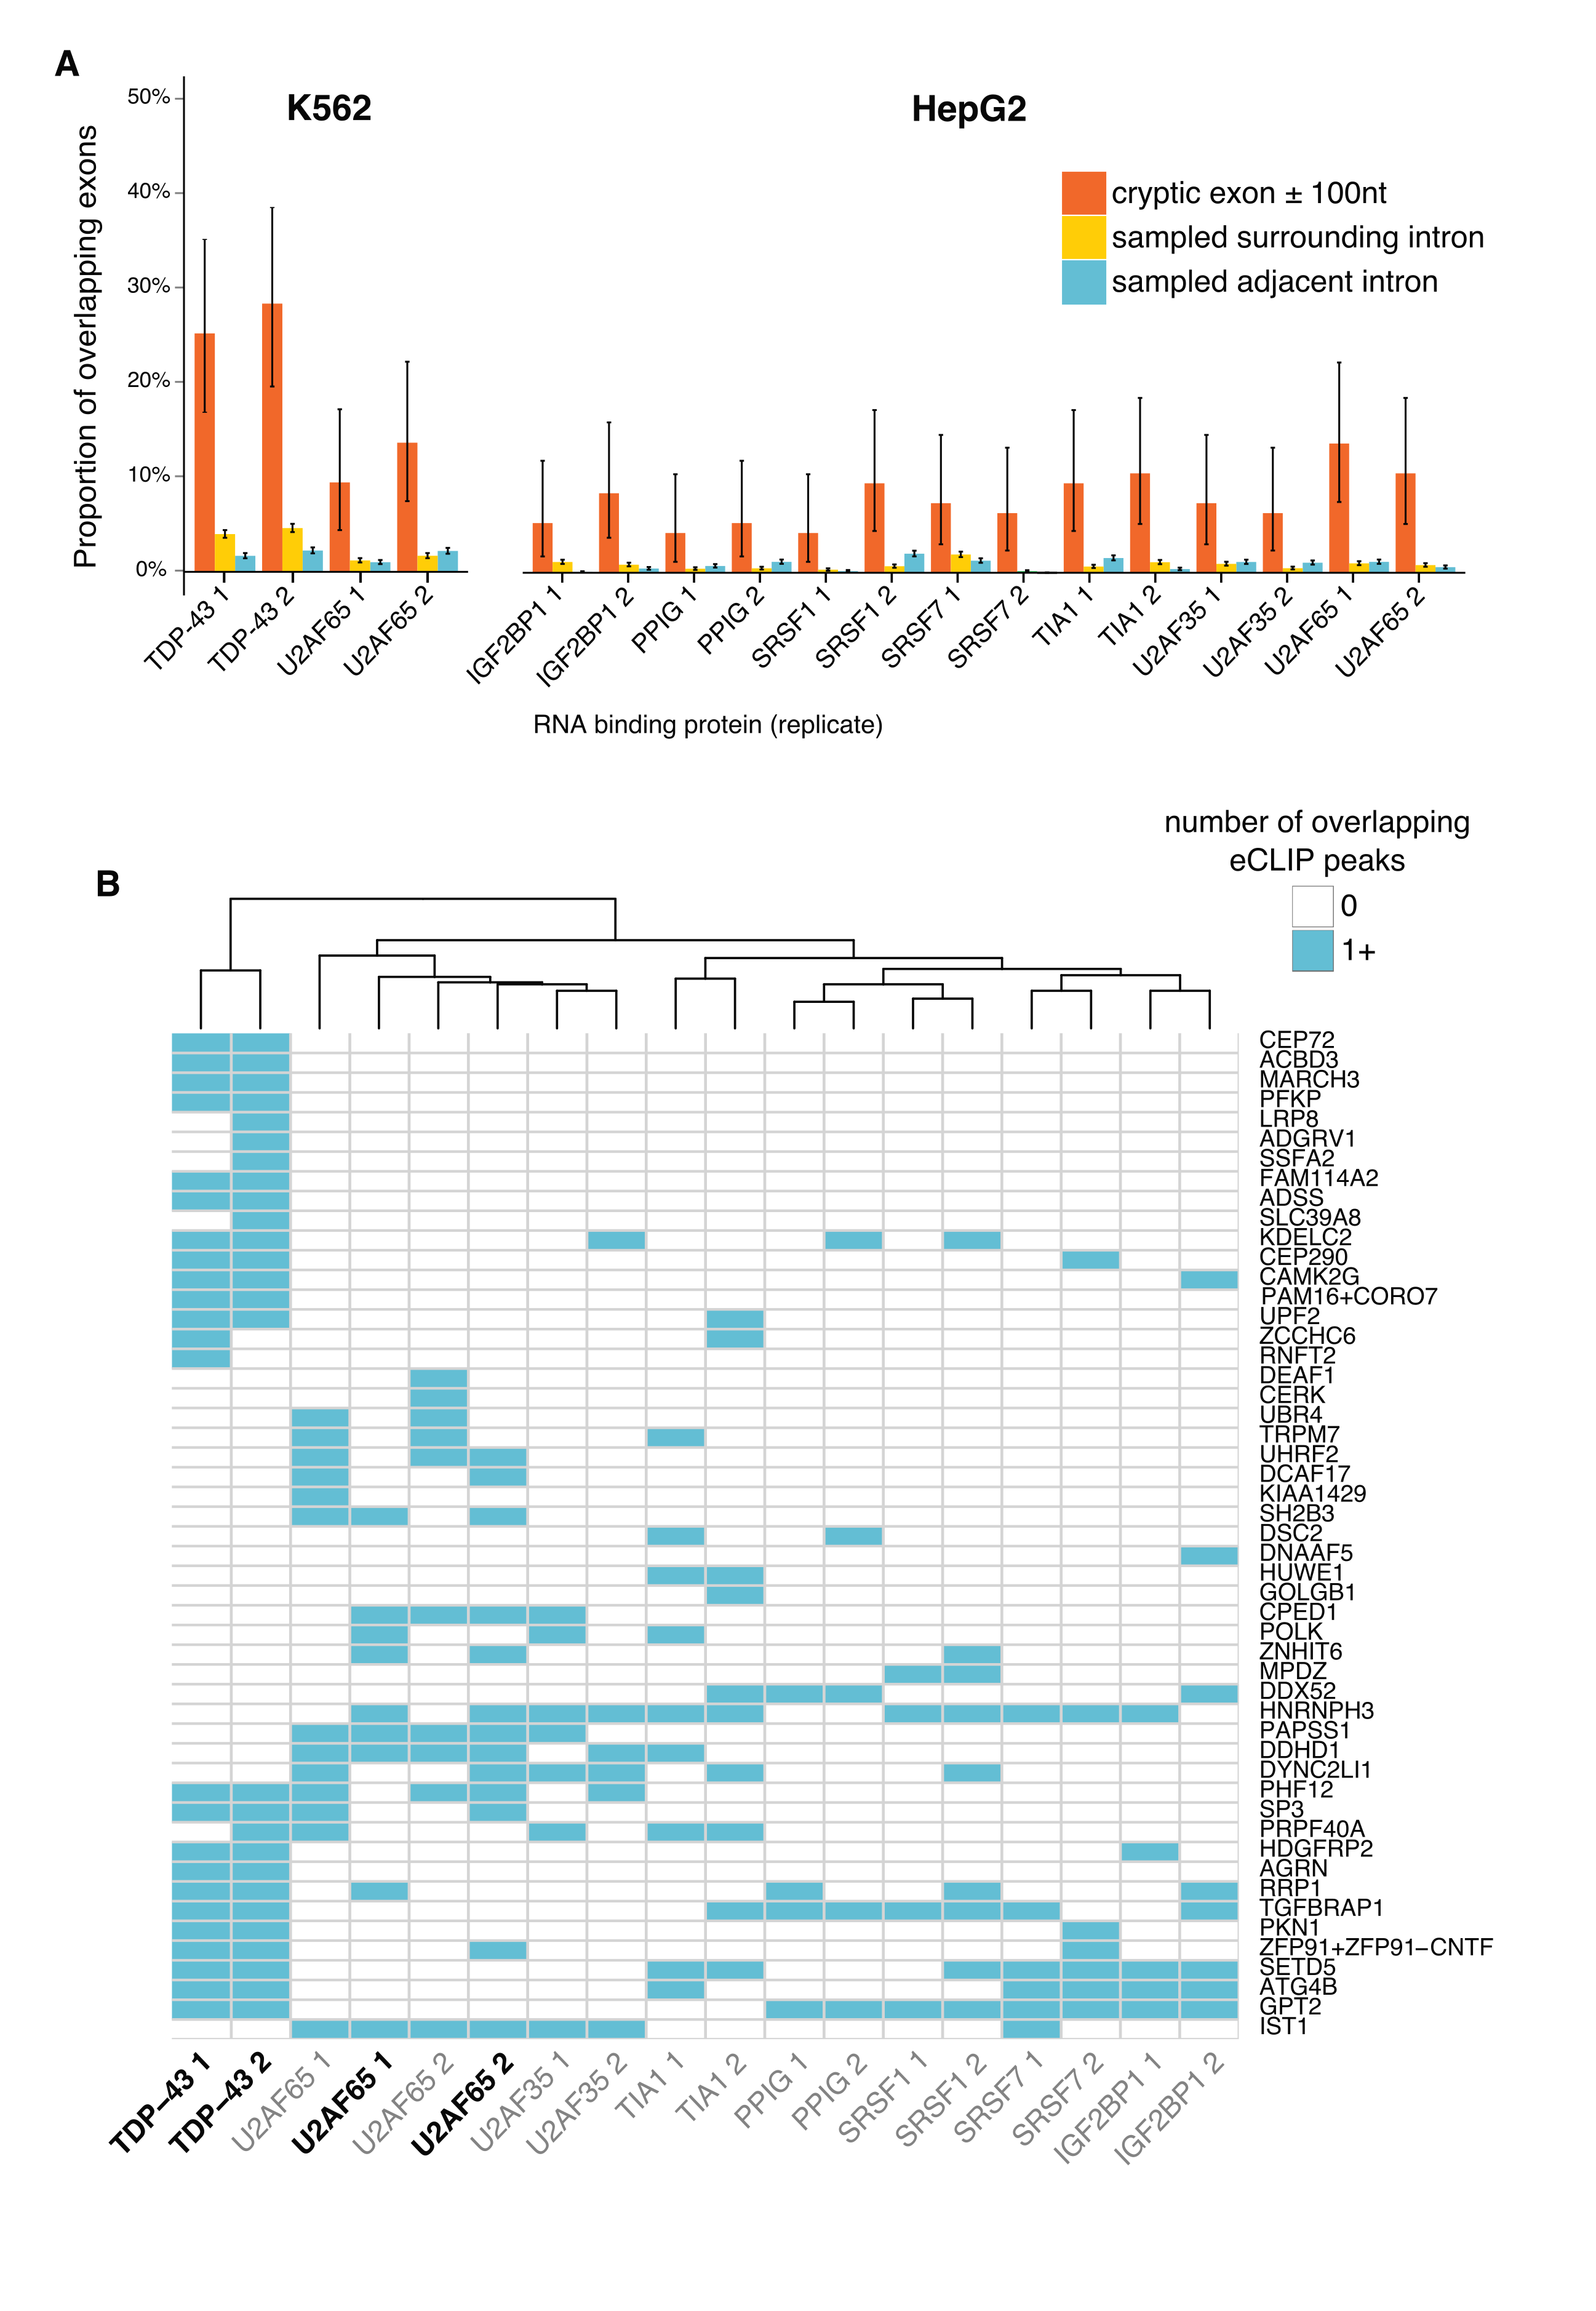
\includegraphics[width=\textwidth]{Figures/03_cryptic_exons/Figure_7_ENCODE_mining.png}
	\caption{\textbf{Mining of ENCODE eCLIP data in K562 and HepG2 cells}}
		A) RNA-binding proteins (RBPs) with significant ($P < 0.05$) proportion of overlapping cryptic exons (red) compared to sampled intronic sequence from the same (green) and adjacent introns (blue). B) Comparison of eCLIP datasets from different RNA binding proteins (columns) showing the overlap with the cryptic exons (rows). RBPs in bold typeface are from K562 cells whereas those in regular typeface are from HepG2 cells.
		\label{fig:cryptic_mining}
\end{figure}

\section{Discussion}
I designed an analytical strategy to identify cryptic splicing that takes advantage of biological replicates in RNA sequencing data. I have applied this tool to a set of human and murine TDP-43 depletion datasets, as well as datasets that deplete hnRNP C or FUS. The results are consistent with the previous findings that depletion of TDP-43 or hnRNP C leads to the inclusion of novel cryptic exons in both human and mouse. Although FUS undoubtedly plays an important role in splicing and mRNA stability and shares a number of targets with TDP-43 \citep{Lagier-Tourenne2012-wa}, the low number of cryptic exons observed due to FUS depletion suggests that it does not play a major role in cryptic splicing and is a key point of differentiation with TDP-43.

Further examination of TDP-43 linked exons suggests they tend to possess the necessary UG-rich sequence elements to be bound by TDP-43 and using iCLIP data I observed that a subset of the cryptic exons are shown to be bound by TDP-43 \emph{in vivo}. I went on to investigate the origins of these TDP-43 bound cryptic exons, as has been done for the targets of hnRNP C. I observed that unlike hnRNP C linked cryptic exons, which invariably originate from antisense Alu elements, TDP-43 linked cryptic exons do not originate from any single family of transposable element. Furthermore their sequences show very low species conservation, akin to random intronic sequence, but remarkably they contain splice sites very close in strength to those of their adjacent annotated exons. Differential expression analysis suggests that the bulk of cryptic exon containing genes are significantly downregulated upon TDP-43 depletion. I hypothesize that this is due to nonsense mediated decay of the inclusion transcript, which I predict would occur in over 90\% of cryptic exon containing transcripts. Comparing my human cryptic exons with a recent proteomic study of TDP-43 depletion in human SH-SY5Y cells \citep{Stalekar2015-qd} showed that protein levels were changed for 3 of the 95 human cryptic exon containing genes. Two, \emph{HUWE1} and \emph{GOLGB1} had protein levels that were 8\% and 31\% of the control cells respectively whereas the third, \emph{HNRNPH3} was found to be 7-fold increased under TDP-43 depletion. Interestingly, the cryptic exon discovered in hnRNP H3 falls upstream of the start codon whereas those found in \emph{HUWE1} and \emph{GOLGB1} are predicted to trigger NMD by inclusion of intronic RNA into the coding sequence (see Supplementary Table 1).  Another gene with cryptic splicing seen in both K562 datasets and in the initial Ling HeLa data, \emph{AGRN}, has been shown to be decreased at the protein level in the cerebrospinal fluid of ALS patients compared to healthy controls and other neurological diseases \citep{Collins2015-xd}. Correct splicing of \emph{AGRN} has shown to be crucial for the formation of the neuromuscular junction \citep{Ruggiu2009-qx}.

My understanding of TDP-43's role in cryptic splicing is that of a safeguard against the inclusion of potentially damaging intronic sequence into transcripts. However, the relationship between the UG-rich sequences and the strong 5\'\ and 3\'\ splice sites and their changes over evolutionary time are unknown as we observed no conserved cryptic exons between human and mouse. 

Using publicly available ENCODE eCLIP data, I identified a number of RNA binding proteins that also bind subsets of human cryptic exons under normal conditions, that is, in the presence of TDP-43.  It is unsurprising that the splicing factors U2AF35 and U2AF65 are enriched as they preferably bind pyrimidine-rich 3\'\ splice site sequences which all cryptic exons appear to possess. That only 10-15\% of cryptic exons show U2AF35/65 binding may be due to competition from TDP-43 in a manner similar to that seen between hnRNP C and U2AF65 \citep{Zarnack2013-nv}. TIA-1 is an exciting finding due to its role in the formation of stress granules, which are key regulators of RNA stability \citep{gilks2004stress}. In addition, IGF2BP1 has been reported to be bound to TDP-43 in HEK293T and HeLa cell extracts \citep{Ling2010-sr,Freibaum2010-hw}, whereas SRSF7 was reported as binding to TDP-43 in mouse N2A cells \citep{Blokhuis2016-hw}. None of the observed proteins have been reported to change their protein level in response to TDP-43 depletion \citep{Stalekar2015-qd}.

As the majority of cryptic exons are predicted to lead to nonsense-mediated decay of the inclusion transcript it seems peculiar that we can observe these transcripts at all. I hypothesise that cryptic splicing may be much more widespread than can be observed by RNA sequencing due to the highly efficient nature of nonsense mediated decay. Over half of all cryptic exon genes are significantly downregulated in each dataset (Fig 3.2B), suggesting that cryptic exon inclusion may be a key mechanism in the widespread changes in RNA expression that occur upon TDP-43 depletion. This has been explored in hnRNP C, where a large increase in the number and observed inclusion of Alu-derived cryptic exons was seen when both hnRNP C and the nonsense mediated decay-associated protein UPF1 were co-depleted compared to just hnRNP C or UPF1 alone \citep{Attig2016}.

Two genes, \emph{ATG4B} and \emph{GPSM2}, have previously been demonstrated to have cryptic exon inclusion RNA transcripts in ALS patient brain samples, suggesting a role for cryptic splicing in disease \citep{Ling2015}. My analysis also identified a cryptic exon in \emph{ATG4B} in human cells, but not \emph{GPSM2}; however I did not analyse human brain data. By expanding the list of cryptic exons, it will be interesting to explore whether these are also dysregulated in ALS patient brains. However, such analysis may prove challenging owing to the likely small concentrations of RNA originating from diseased cells in brain homogenate and the likelihood of degradation by NMD. Alternate strategies may involve mass spectrometry screens for the subset of cryptic exon containing genes that escape the NMD process, for example because the cryptic exon is in frame. Such proteins may represent useful biomarkers for ALS. 

A recent paper has used a complementary bioinformatic method to increase the number of cryptic exons seen in the original Ling data \citep{Tan07102016}. This study extends the cryptic splicing phenomenon to RBM17, another RNA-binding protein, making the very low number of cryptic exons observed in the FUS depletion datasets even more surprising,

Defining cryptic exons by their absence in existing annotation is not a suitable long term strategy. For example, the \textit{SORT1} gene contains an exon normally repressed by TDP-43 and not constitutively included in any tissue \citep{Prudencio2012}. But due to the studies that have documented its existence the "cryptic" exon in SORT1 is annotated in all transcript databases. There are certainly many examples of annotated exons that are extremely rarely included and may be repressed by splicing factors like TDP-43. Future studies may have to take a more measured approach based on the frequency of inclusion in multiple tissues and conditions to assess whether an exon is truly cryptic or not.


\section{Summary}
In this project I replicate and confirm the presence of cryptic exons after TDP-43 depletion and show they have a negative impact on the genes they reside in, leading to decreased expression levels. Further work is warranted to determine the relevance of cryptic exons to ALS and FTD pathogenesis.



%\chapter{FUS mutant mice show progressive changes in mitochondrial and ribosomal transcripts}

\label{chapter:fus_mouse}

Work presented in this chapter has been published as part of \citep{Devoy2017}. See appendices for full reproduction of the published manuscript.

\section{Overview}
This chapter describes work carried out in collaboration with Dr Anny Devoy of the UCL Institute of Neurology. 
Dr Devoy created a "humanised" mouse model of ALS resulting from a mutation in the FUS RNA-binding protein. 
I analysed RNA-seq taken from two tissues and time points and demonstrated a specific transcriptomic signature that correlates with a progressive neurodegenerative phenotype seen in aged mutant mice.
This involves the downregulation of mitochondrial and ribosomal transcripts.

\section{Contributions}
\begin{itemize}
	% Check with Pietro
	\item Transgenic mice were created by Dr Anny Devoy
	\item RNA sequencing libraries were prepared by Dr Anny Devoy
	\item RT-PCR validation was performed by Dr Anny Devoy
	\item Fig. \ref{fig:delta14_structure} was created by Dr Anny Devoy
\end{itemize}
All bioinformatic analysis and interpretation was designed and performed by myself in consultation with Dr Anny Devoy and my supervisors. 


\section{Background}
% REWRITE
All previous studies alter FUS expression to levels that wildly differ to the normal biological situation. Overexpression or knockout are clearly toxic but these do not help to differentiate the effects of the mutations of normal FUS function. 
%recently
Until recently there have been no studies where the effects of a human FUS mutation are seen on the mouse at a physiological level of expression. 
The FUS $\Delta$14 mutation was found in an early onset ALS patient who died at the age of 22 following a very rapid disease course \citep{DeJesus-Hernandez2010}. The mutation alters the 3\'\ splice site of exon 14 of FUS, causing it to be skipped.  Comparison of the $\Delta$14 mutation with other, late-onset ALS causing mutations have shown an increased propensity by FUS $\Delta$14 to accumulate in the cytoplasm \citep{Verbeeck2012}. Analysis of mice carrying a single copy of the FUS $\Delta$14 mutation enables a reconstruction of progressive neurodegenerative disease. By analysing RNA-seq data collected across the lifespan of the mice, I can observe specific RNA dysregulation caused by the mutant protein.

\subsection{The FUS $\Delta$14 mouse is a humanised model of ALS}
The FUS $\Delta$14 mouse was created by directed mutagenesis of the mouse Fus exon 14 splice site as well as humanisation of exon 15 with 4 separate mutations.The result of splicing exons 13 and 15 together is a frameshift which at the protein level removes the C-terminal nuclear localisation signal (Fig. \ref{fig:delta14_structure}A) but leaves a novel peptide sequence which can used to create specific antibodies. Reverse-transcription PCR to detect FUS mRNA showed the $\Delta$14 FUS mRNA to be expressed at a similar level to wildtype FUS (Fig. \ref{fig:delta14_structure}B). 


\begin{figure}[h!]
	\begin{center}
		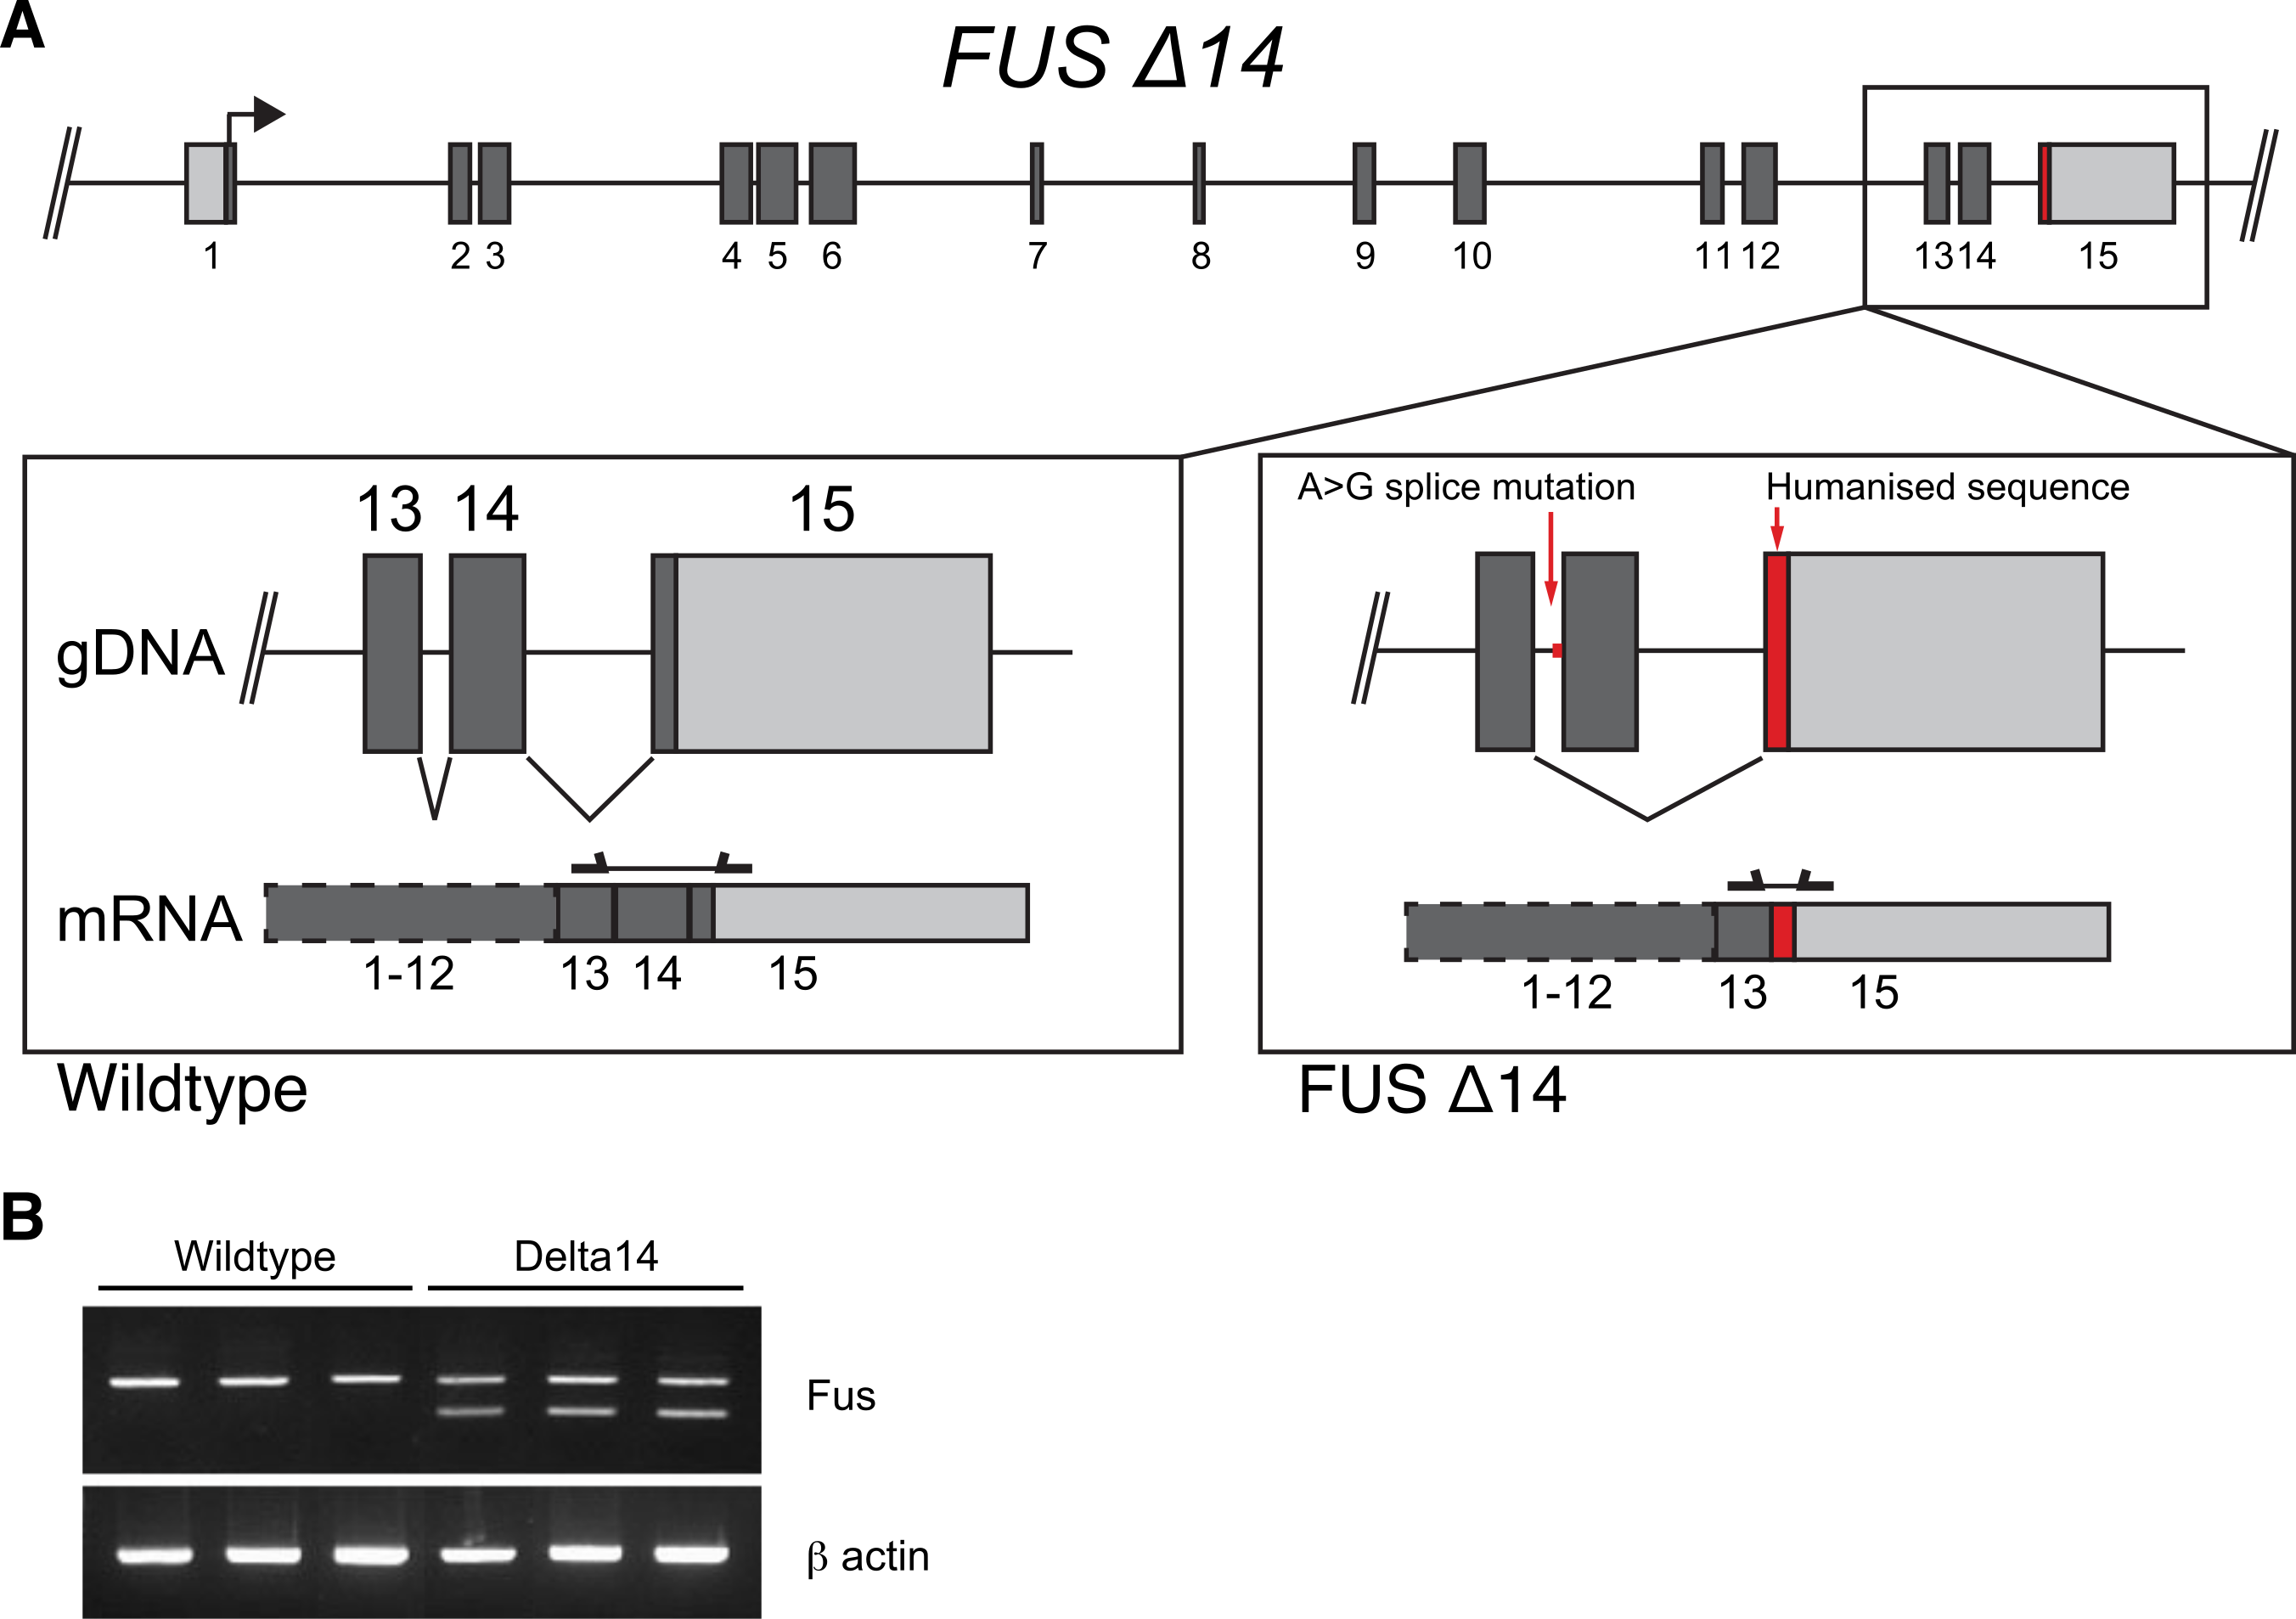
\includegraphics[width=\textwidth]{Figures/04_fus_mice/anny_FUS_schematic.png}
	\end{center}
	\caption[The FUS $\Delta$14 model]{
		\textbf{The FUS $\Delta$14 model.}
		\textbf{(A)} The FUS locus with a closeup of the terminal three exons in the wildtype mouse (left) and the FUS $\Delta$14 mouse (right). 
		\textbf{(B)} RT-PCR of FUS mRNA from spinal cord of wildtype and mutant mice.
	}
		\label{fig:delta14_structure}
\end{figure}


\section{Methods}

\subsection{Data preparation}
All RNA-seq data used is listed in table \ref{table:fus_mice_rnaseq}. All samples were aligned to the mm10 mouse reference genome using the previously discussed analysis pipeline.


\begin{table}[h!]
	\caption[All RNA-sequencing data used in this study]{
		\textbf{All RNA-sequencing data used in this study}
	Library info describes the type of library prepared, the length of each read and whether the sequencing was single or paired end. PE: paired end sequencing. Depth is defined the number of uniquely mapped read pairs, in millions.
}
	\label{table:fus_mice_rnaseq}
	\begin{center}
		\begin{small}
			\begin{tabular}{llllp{1.5cm}llll}
				Species & Cell type & Time point & Library info & Depth & Number\\
				\hline
				Mouse & Spinal Cord & 3 months & stranded mRNA 75bp PE & 33-43M & 4 vs 4\\
				Mouse & Spinal Cord & 12 months & stranded mRNA 75bp PE & 35-46M & 4 vs 4\\ 
				Mouse & Motor/Frontal Cortex & 3 months & stranded mRNA 75bp PE & 35-52M & 4 vs 4\\
				Mouse & Motor/Frontal Cortex & 12 months & stranded mRNA 75bp PE & 35-48M & 4 vs 4\\ 
			\end{tabular}
		\end{small}
	\end{center}
\end{table}

\subsection{Differential gene expression}
Differential expression was carried out with \textit{DESeq2} \citep{Love2014} comparing wildtype with mutant mice. All P-values were adjusted at a false discovery rate of 10\%. To assess the variance between each sample the raw counts for each gene were normalised to account for library size and then normalised again by the regularized log normalisation method \citep{Love2014}. The counts were further transformed into Z-scores, which express the number of standard deviations from the mean of all counts for that gene. Heatmaps were created for all significantly differentially expressed genes using the \textit{pheatmap} R package \citep{Kolde2012}.  

\subsection{Gene Ontology analysis}
Gene ontology (GO) analysis is a method to extract inference from gene expression experiments by annotating each gene and protein within a unified vocabulary of molecular and cellular function. This can be used to identify dyregulated pathways or broader trends \citep{Ashburner2000}. For each differential expression results set the multiple correction threshold was dropped to P < 0.005 for each gene to increase the number of input genes. The resulting list of hits was then annotated for GO terms and a hypergeometric test was applied to test the enrichment of particular categories against a background set of genes. It is important to account for selection bias for long genes in RNA-seq data as longer genes have more power to be differentially expressed than shorter genes \citep{Young2010}. The R package \textit{GOseq} implements a GO term annotation and enrichment test which takes account of this length bias \citep{Young2010}. The resulting P-values were then Bonferroni corrected for multiple testing. In each category the number of genes that were up- or downregulated in the $\Delta$14 mice relative to wildtype littermates were expressed as a percentage. 

\subsection{Differential splicing}
Differential splicing was analysed for the 12 month spinal cord samples using SGSeq \citep{Goldstein2016} to find novel and annotated splicing events. Counts of inclusion and exclusion were used to fit a model with DEXSeq \citep{Anders2012} to test the effect of condition on splicing event inclusion. Splicing events were reported at FDR < 0.05.

\section{Results}

\subsection{Gene expression changes are tissue- and time point-specific}

\begin{figure}[h!]
	\centering
	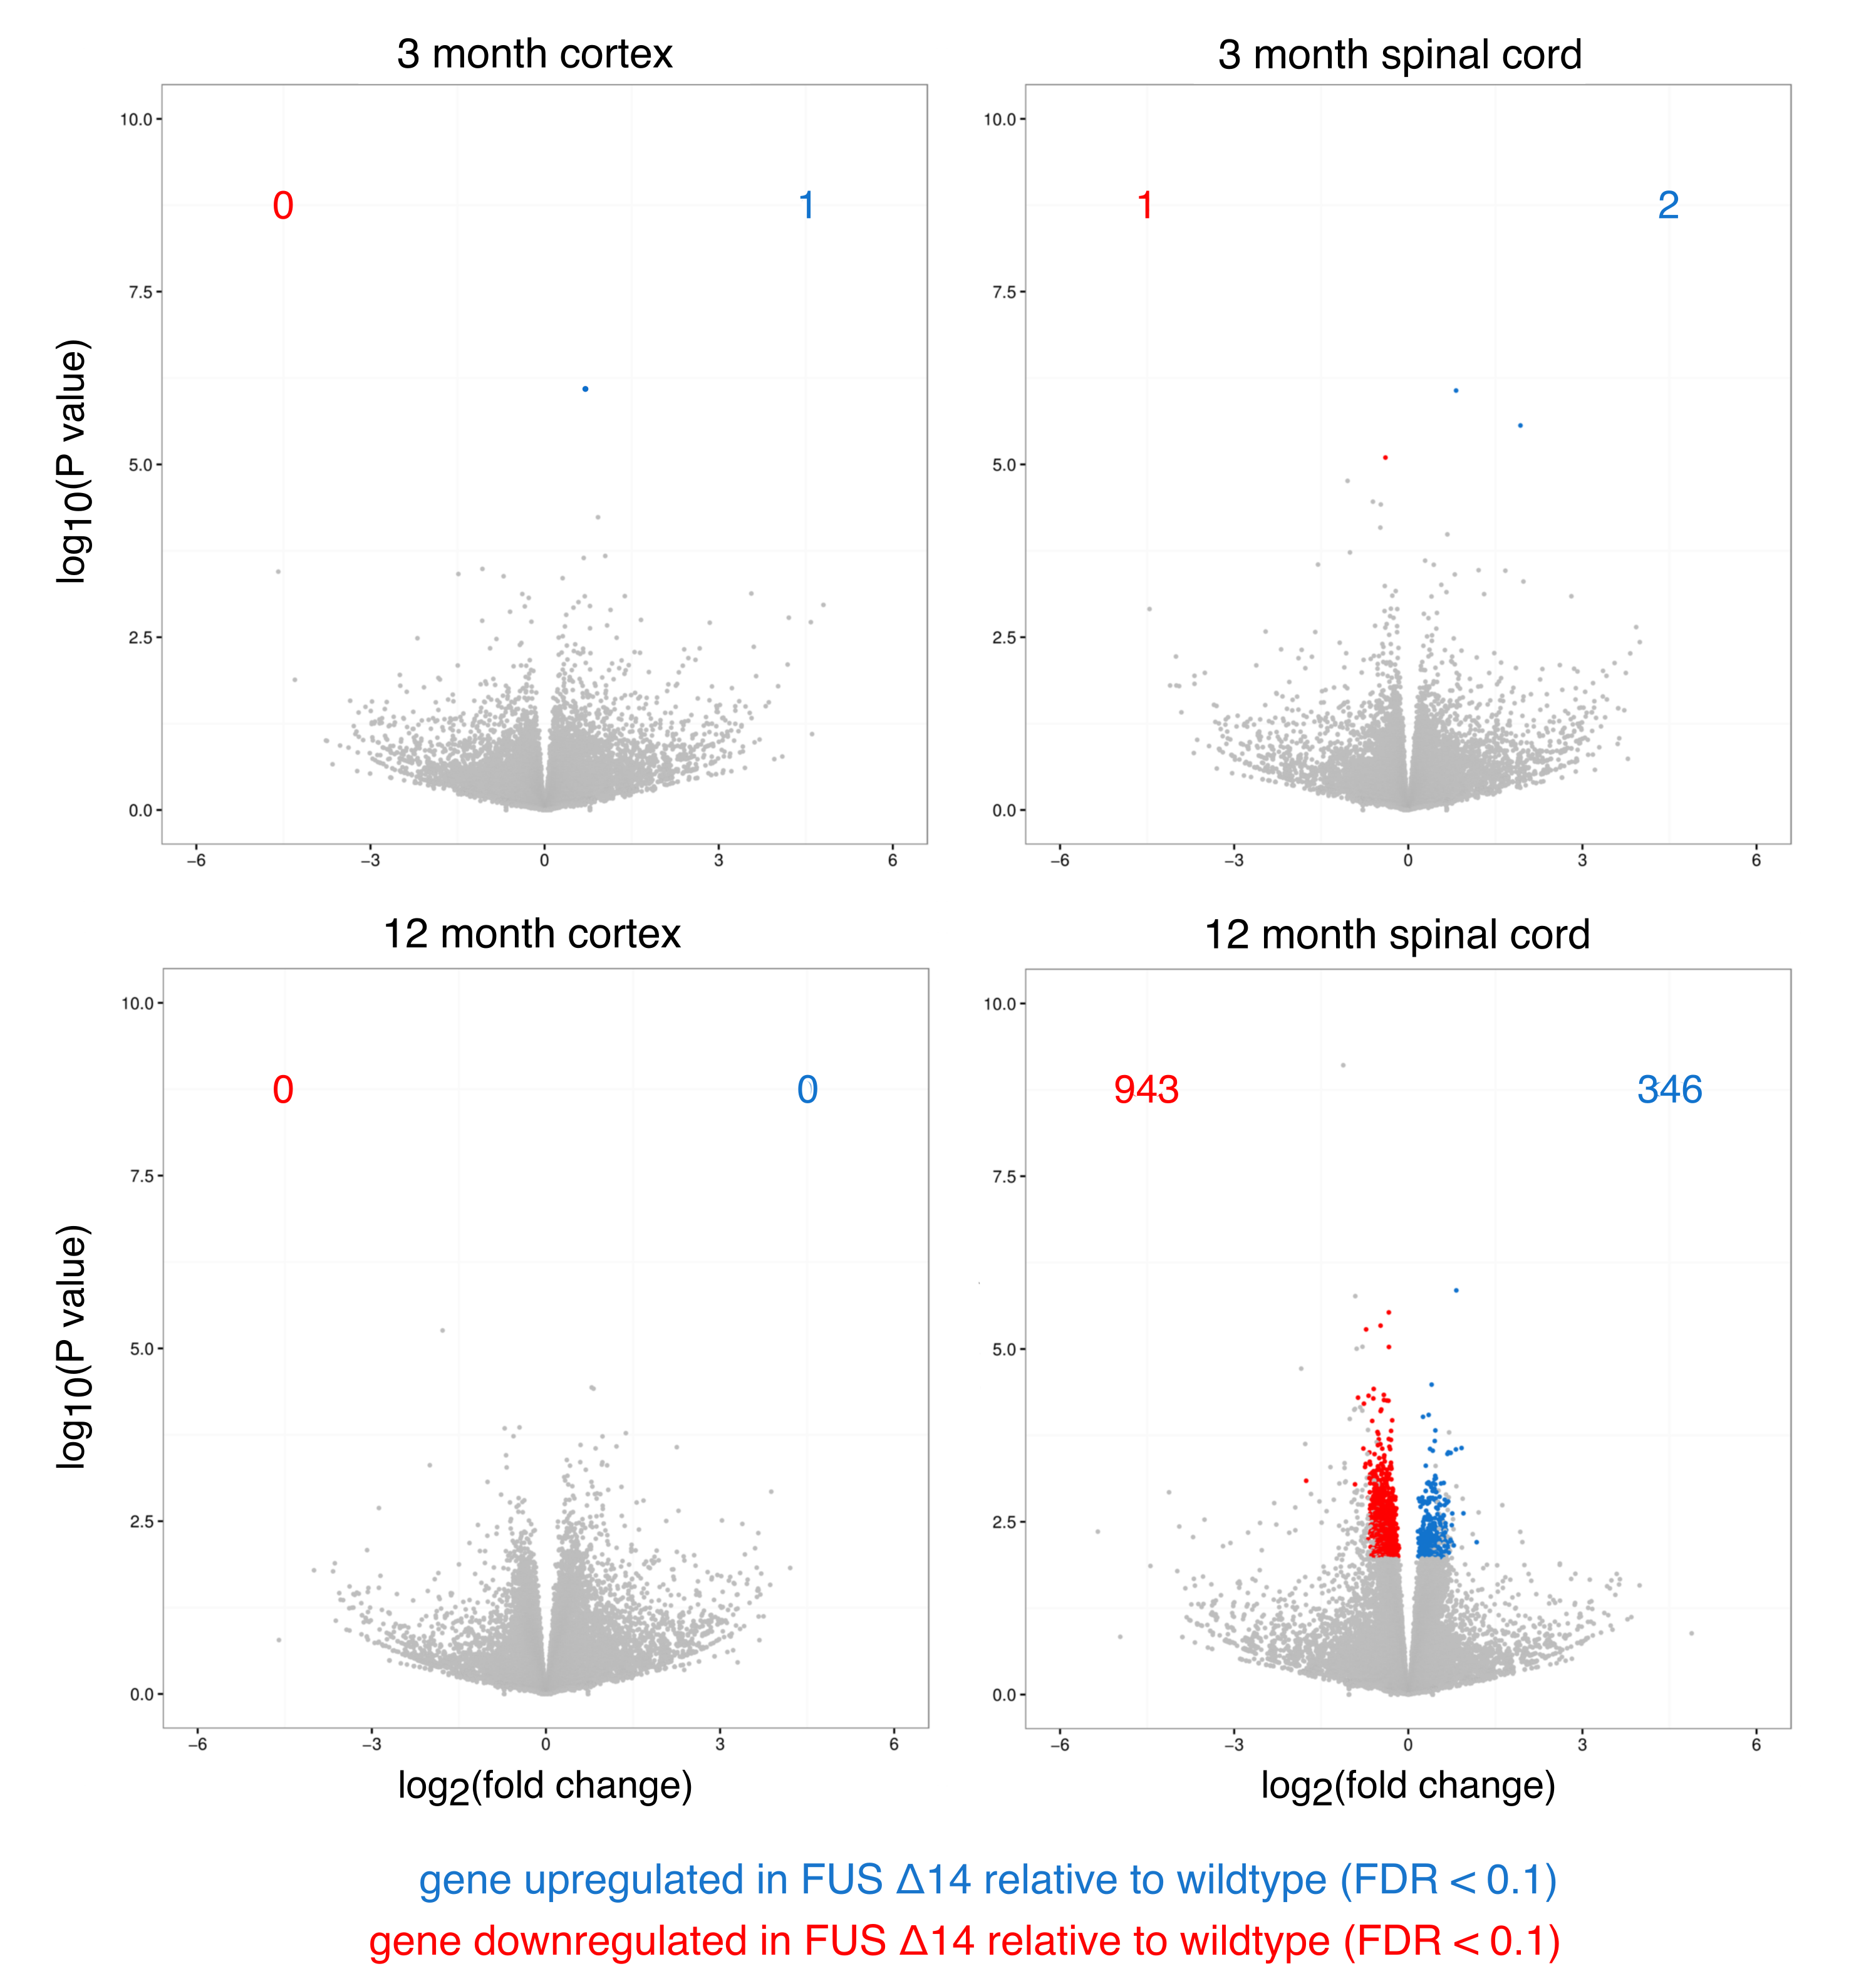
\includegraphics[width=\textwidth]{Figures/04_fus_mice/anny_volcanos.png}
	\caption[Differential gene expression analysis on the $\Delta$14 mouse]{
		\textbf{Differential gene expression analysis on the $\Delta$14 mouse across two tissues and time points.}
		Each gene is represented as a point. The x axis is the $log_2$ of the ratio between the average expression in the $\Delta$14 mice against that of the wildtype mice. The y axis is the $log_10$ of the unadjusted P-value for the differential expression test. The numbers of upregulated genes (adjusted \textit{P} < 0.1 with a $log_2$(fold change) > 0) are in blue and the the downregulated ( adjusted \textit{P} < 0.1 with $log_2$(fold change) < 0) are in red.
	}
	\label{fig:delta14_volcanos}
\end{figure}

To examine progressive changes in RNA regulation, total RNA was extracted from both spinal cord and forebrain from mice across two time-points: 3 months and 12 months. Four male mice of each genotype ($\Delta$14 and wildtype littermate) were used at each timepoint. At 3 months of age, the forebrain and spinal cord samples had 1 and 3 genes differentially expressed respectively. At 12 months of age there were no differentially expressed genes found in the forebrain but 1,289 found in the spinal cord, with genes predominantly decreased in expression (Fig. \ref{fig:delta14_volcanos}). To examine the variance between each sample in the 12 month spinal cord dataset, the read counts for each gene were normalised and converted to Z-score values. Plotted as a heatmap it is clear that the size of each change is small and there is considerable inter-condition variability (Fig. \ref{fig:delta14_heatmap}).


\begin{figure}[h!]
	\centering
	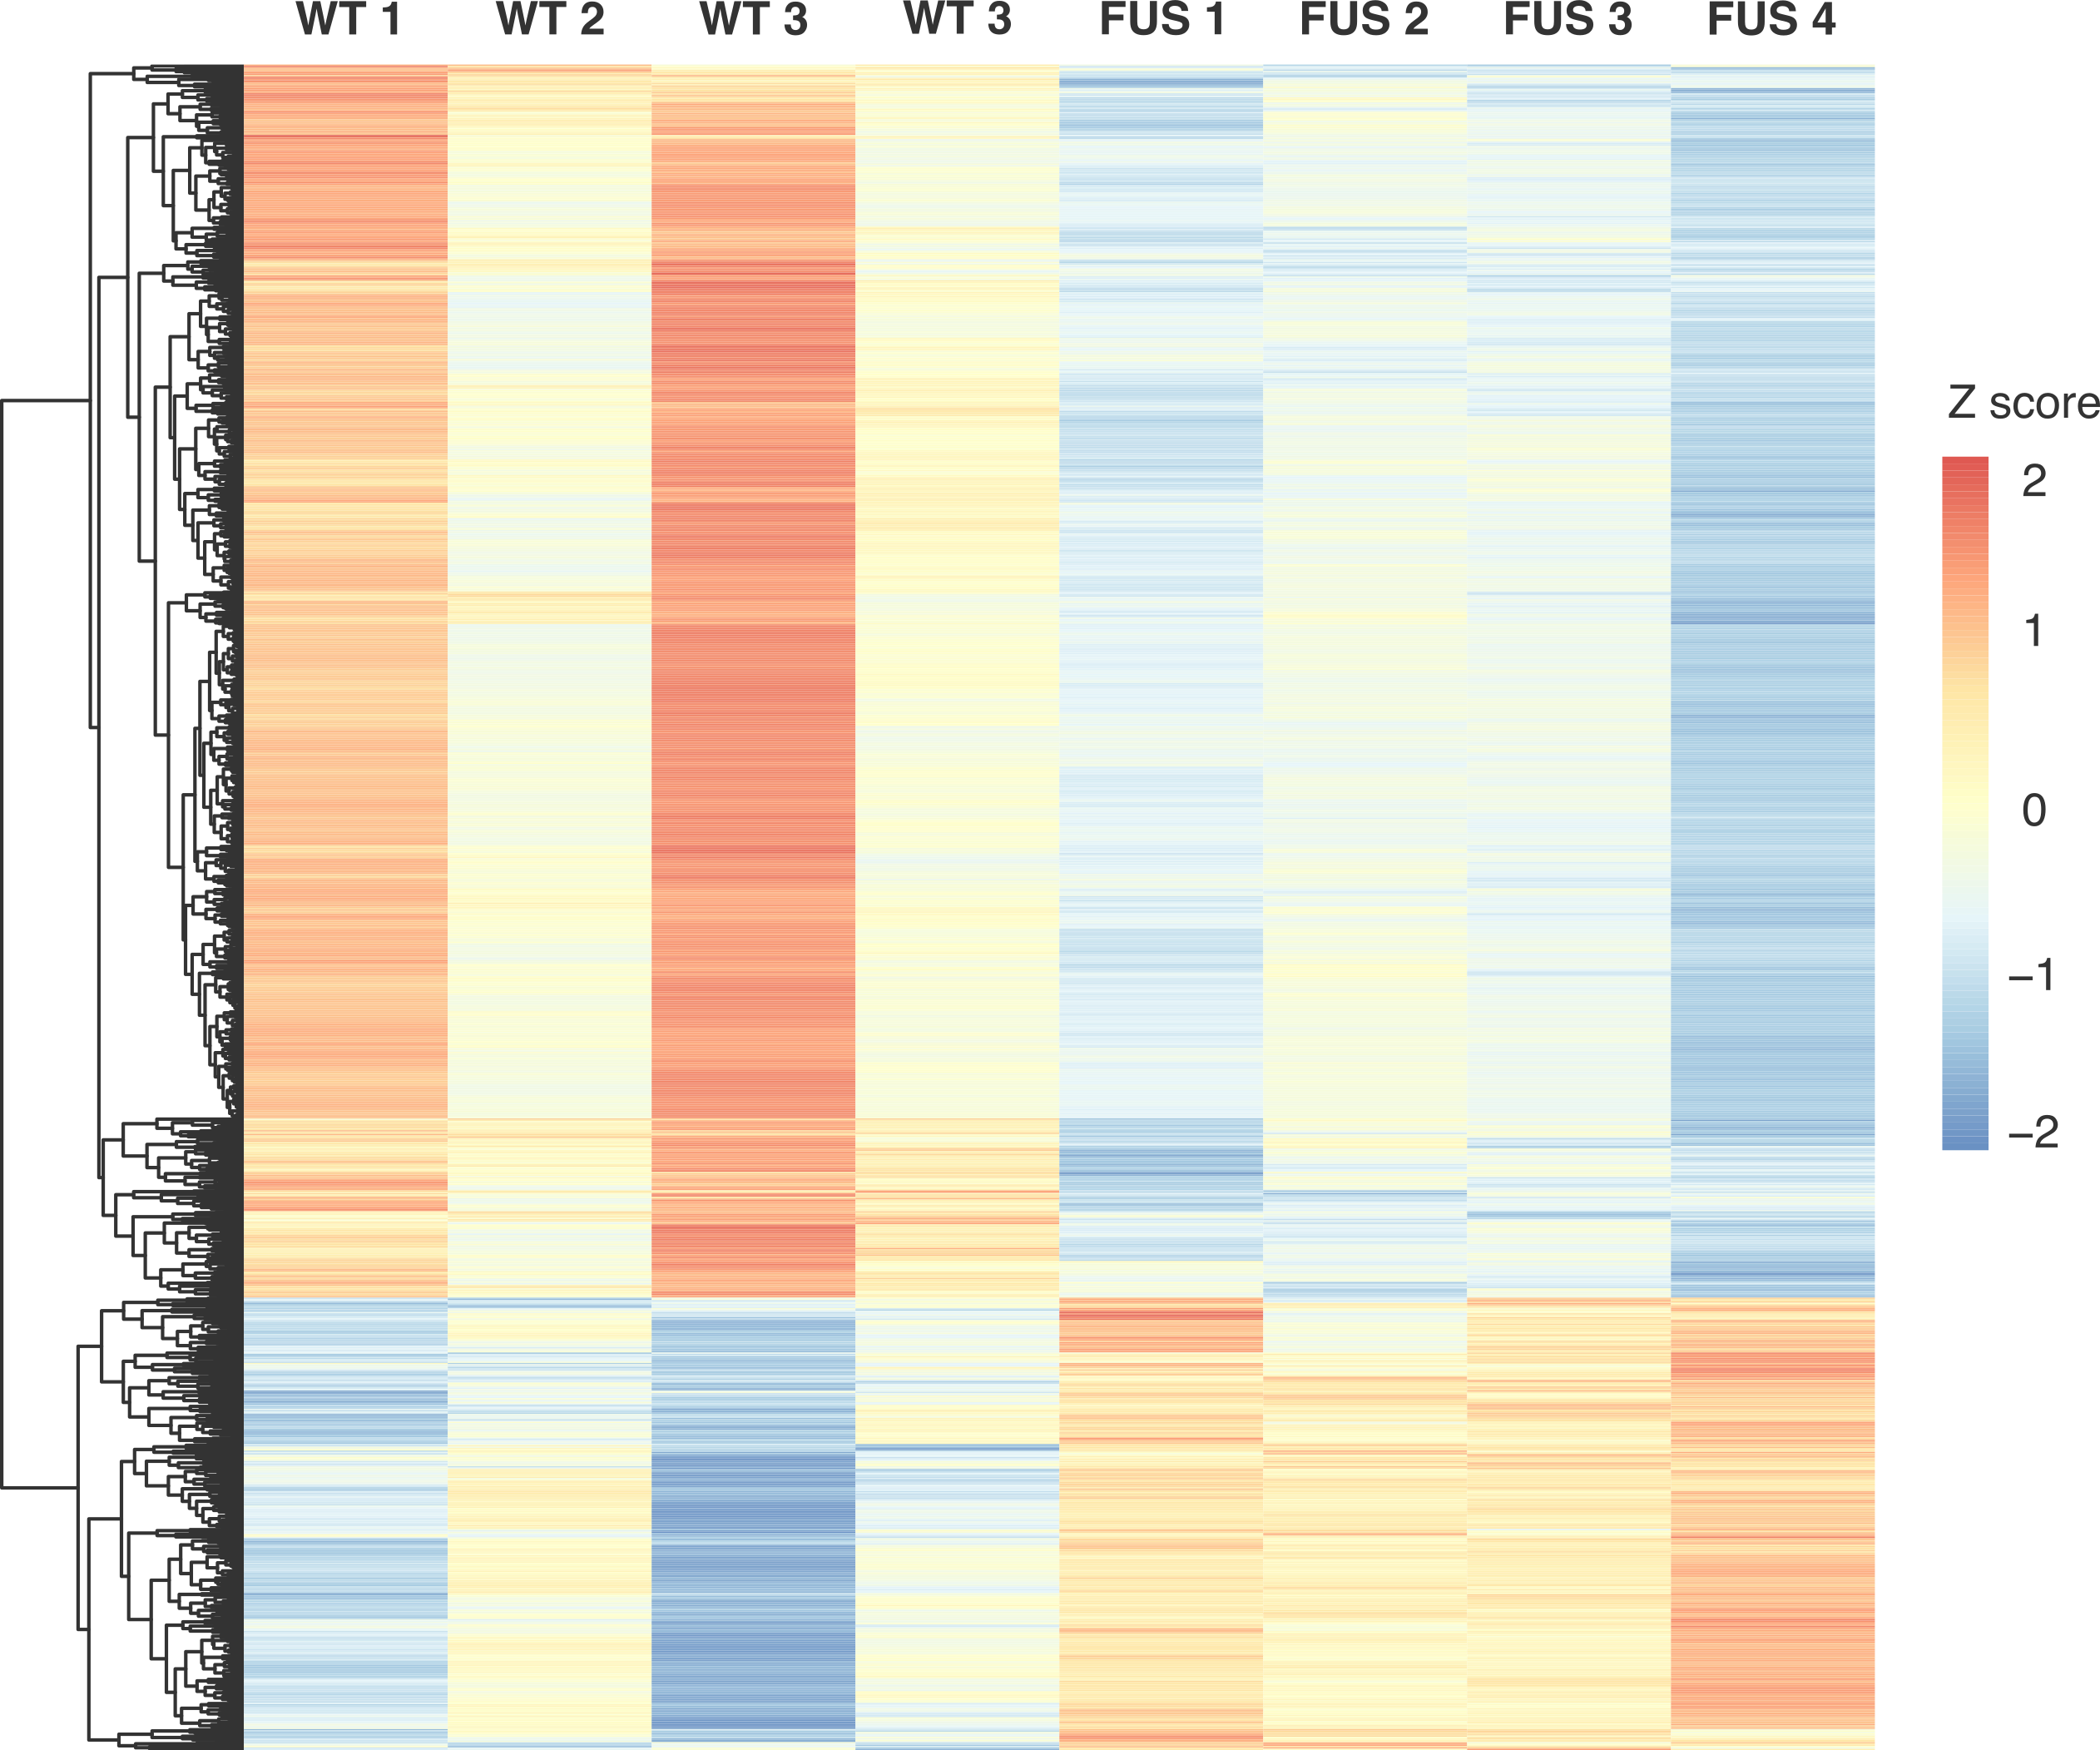
\includegraphics[width=\textwidth]{Figures/04_fus_mice/anny_normalised_heatmap.png}
	\caption[Z-score heatmap of the 12 month spinal cord dataset]{
		\textbf{Z-score heatmap of the 1289 differentially expressed genes in 12 month spinal cord dataset}
	WT: wildtype littermate; FUS: FUS $\Delta$14 heterozygote. 
}
	\label{fig:delta14_heatmap}
\end{figure}


\subsection{Gene ontology analysis indicates changes in mitochondrial and ribosomal pathways}
Genes from the 12 month spinal cord dataset differentially expressed at a relaxed threshold of \textit{P} < 0.005 were sent for gene ontology enrichment analysis. This compares the number of genes that are members of a particular ontology category with the expected distribution. This analysis identified a strong enrichment in genes belonging to mitochondria, ribosome and proteasome cateogories. Strikingly, almost all the genes in these categories were downregulated (Fig. \ref{fig:delta14_go}).

\begin{figure}[h!]
	\centering
	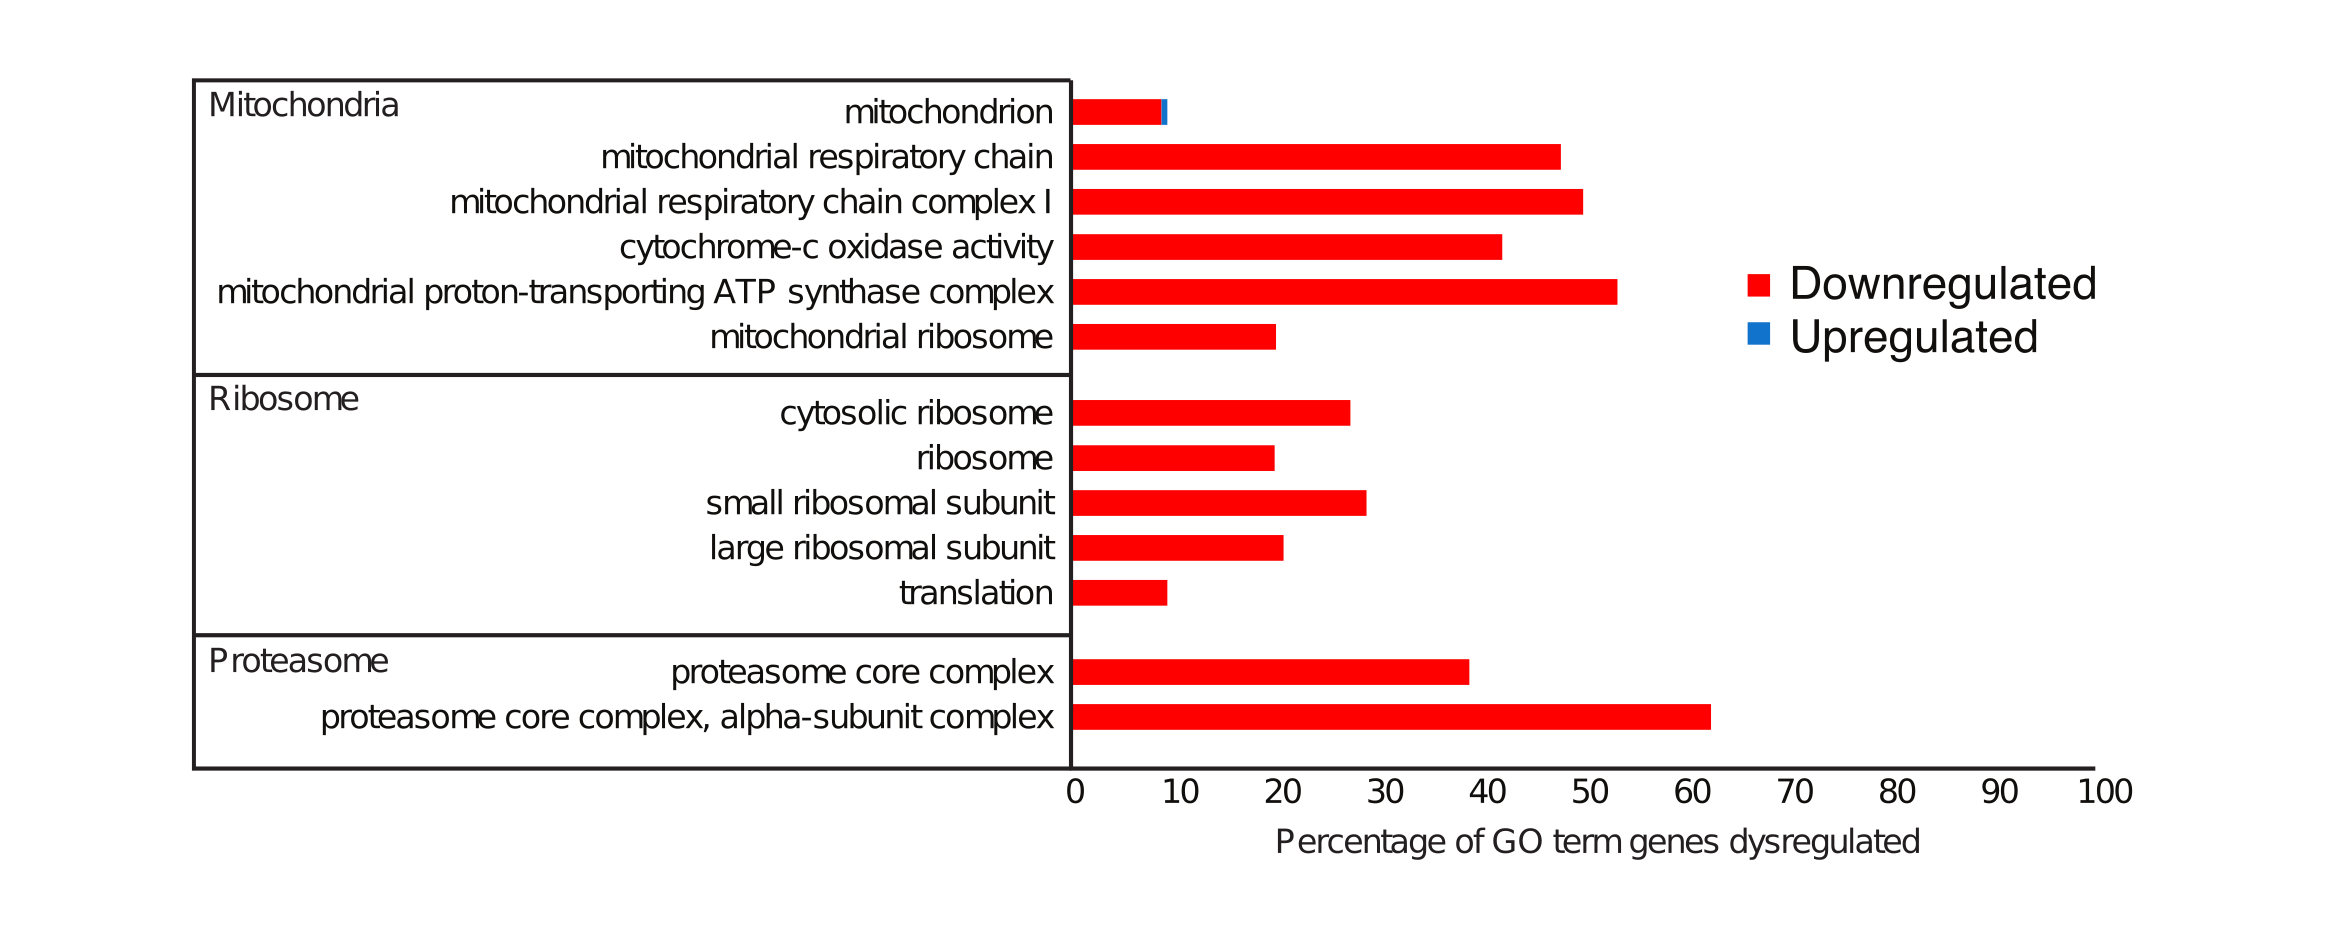
\includegraphics[width=\textwidth]{Figures/04_fus_mice/anny_GO_terms.png}
	\caption[Gene ontology categories in the 12 month spinal cord samples]{
		\textbf{Gene ontology categories significantly enriched in the 12 month FUS $\Delta$14 spinal cord samples}
		Each significant gene ontology category ( adjusted P < 0.05) is expressed as a proportion of upregulated (red) or downregulated (blue) genes.
	}
		\label{fig:delta14_go}
\end{figure}


\subsection{Splicing events are limited to FUS itself and few other genes}
Due to the lack of gene expression changes seen in other comparisons, differential splicing was assessed on 12 month spinal cord samples only.  
11 splicing events were found at FDR < 0.05, 4 of which were found in \textit{Fus} itself.
The top 2 splicing events in \textit{Fus} overlap exon 14, the skipping of which in the $\Delta$14 mice is classified as both an alternative last exon and an alternative start site.
The latter is a mis-annotation by \textit{SGSeq} due to the poor mappability of the central sequence of exon 14, leading to a gap in reads that span both ends of the exon.
The other 2 splicing events in \textit{Fus} are in the middle of the transcript where two introns, 6 and 7, are retained more in the wildtype mice and less retained in the $\Delta$14 mice.
Two overlapping complex events are seen in the \textit{Mbp} gene which encodes for Myelin basic protein, a major component of the myelin sheath. \textit{Mbp} is alternatively spliced to create different isoforms \citep{DeFerra1985}. A complex event involving 4 cassette exons is subtly altered in $\Delta$14.
\textit{Ewsr1} is a closely-related RNA-binding protein that interacts with FUS at the protein and RNA level \citep{Kapeli2016,Lagier-Tourenne2012}. 
A novel intron retention event in \textit{Ewsr1} is retained less in FUS $\Delta$14 mice.
This may in fact be a differential polyadenylation event that has previously been observed \citep{Rogelj2012} and mis-classified by the splicing software.
The other splicing events found affect 4 other genes of unknown significance.

\begin{table}[!htbp] 
	\centering 
	\caption[Splicing events found in 12 month spinal cord samples]{
		\textbf{Splicing events found in 12 month spinal cord samples}
	All splicing events found comparing FUS $\Delta$14 mice to wildtype at FDR < 0.05. 
	$log_2$FC: $log_2$ fold change.
	}
	\label{tab:fus_mouse_splicing} 
	\begin{tabular}{@{\extracolsep{5pt}} llccl} 
		\\[-1.8ex]\hline 
		\hline \\[-1.8ex] 
		Gene & type & $log_2$FC & FDR & coordinates (mm10)\\ 
		\hline \\[-1.8ex] 
		\textit{Fus} & alternate last exon & $-0.132$ & $1e^{-118}$ & chr7:127981291-127981458 \\ 
		\textit{Fus} & alternate start site & $-0.413$ & $1e^{-116}$ & chr7:127981522-127981791 \\ 
		\textit{Fus} & retained intron & $-0.217$ & $1e^{-13}$ & chr7:127974434-127975888 \\ 
		\textit{Fus} & retained intron & $-0.191$ & $1e^{-6}$ & chr7:127972770-127974400 \\ 
		\textit{Mbp} & complex  & $-0.014$ & $0.007$ & chr18:82575633-82584116 \\ 
		\textit{Mbp} & complex & $0.022$ & $0.007$ & chr18:82575633-82584112 \\ 
		 \textit{Ewsr1} & retained intron & $-0.066$ & $0.014$ & chr11:5079485-5078952 \\ 
		\textit{Cyhr1} & alternate 3\'\ splice site & 0.127 & $0.028$ & chr15:76659955-76659439 \\ 
		\textit{Gm32856} & alternate 3\'\ splice site & $-0.317$ & $0.038$ & chr8:129281397-129282476 \\ 
		\textit{Cd47} & cassette exon & 0.148 & $0.038$ & chr16:49906812-49910869 \\ 
		\textit{A330023F24Rik} & retained intron & 1.420 & $0.044$ & chr1:195021564-195021688 \\ 
		\hline \\[-1.8ex] 
	\end{tabular} 
\end{table} 

% 1 and 2 are due to delta 14 splicing
% mis-annotated as alternate start due to low mappability of exon 14


\section{Discussion}
My gene expression analysis demonstrates a progressive and tissue-specific change in RNA regulation, with 1,289 genes differentially expressed in the spinal cord of 12 month mutant mice. This finding is complemented by other contributions to the project. Behavioural experiments have shown the $\Delta$14 mice to have a progressive loss of motor function that is observable from 12 months of age. In addition, a reduction in number of motor neurons in the lumbar spinal cord has been observed from 12 months onwards, accompanied by an increase in cytoplasmic mislocalisation specifically of the mutant FUS.
The broad downregulation of mitochondrial, ribosomal and proteasomal genes specifically in the spinal cord of late-stage mice is an interesting finding that deserves further investigation. 
A recent study of a mouse model where mouse FUS was entirely replaced by either wildtype or ALS mutant human FUS showed similar downregulation of ribosomal (but not mitochondrial) genes \citep{Lopez-Erauskin2018}.
An enrichment of mitochondrial GO categories was previously seen in a FUS knockdown experiment conducted in human embryonic kidney cells  \citep{Schwartz2012}, suggesting that mitochondrial changes may be due to a loss of normal FUS function. Mitochondrial defects have been observed in the brains of FTD-FUS patients accompanied by FUS translocating to mitochondria \citep{Deng2015}. FUS overexpression has also been observed to cause mitochondrial defects at the neuromuscular junction \citep{So2018}. This points to an important role for FUS in mitochondria that may be perturbed by the $\Delta$14 mutation.
As mutant FUS has been shown to impair axonal transport \citep{Guo2017}, this impairment could explain the changes seen in both ribosomal and proteasomal transcripts.
% mitochondrial and ribosomal changes - new papers!

FUS knockout and knockdown experiments have demonstrated that large numbers of splicing events are sensitive to FUS protein levels \citep{Rogelj2012,Lagier-Tourenne2012,Ishigaki2012,Honda2014,Scekic-zahirovic2016}. The small number of splicing events found in the 12 month spinal cord samples suggest that the $\Delta$14 mutation has little affect on splicing with the exception of the \textit{Fus} transcript itself. The two \textit{Fus} intron retention events seen to be less retained in $\Delta$14 compared to wildtype as well as the events seen in \textit{Mbp} and \textit{Ewsr1} are deserving of further study. Defects in myelination have been seen in another FUS NLS mutation \citep{Scekic-zahirovic2017} and this may explain the changes seen in the myelin component \textit{Mbp}. The fellow FET family member \textit{Ewsr1} is also mis-spliced in FUS $\Delta$14. As it is also an intron retention event which changes in the same direction as those seen in \textit{Fus}, this could imply a connection between FUS and \textit{Ewsr1} at the RNA level.
%\chapter{Loss and gain of TDP-43 splicing function in two mutant mouse lines}
\label{chapter:tdp_mice}

Work presented in this chapter has been published as part of \citep{Fratta2018}. See appendices for full reproduction of the published manuscript.

\section{Overview}

TDP-43 is a ubiquitously expressed RNA-binding protein with multiple roles in RNA processing including mRNA splicing.
TDP-43 mislocalisation and aggregation is a common ALS pathology observed in the majority of patient brains.
Additionally, rare  TDP-43 mutations are causative for ALS. 
How TDP-43 mutations lead to disease and how TDP mislocalisation occurs in the absence of mutations is unknown. 
Whether loss of TDP-43 from the nucleus or a gain of TDP-43 in the cytoplasm is the pathological consequence is also under debate.
TDP-43 Mutations cluster in the low-complexity domain of the protein which has been implicated in aggregation and interaction with other proteins.

We generated two mutant mouse lines to study different aspects of TDP-43's role in mRNA splicing.
By comparing the two we discovered that mutations in the low-complexity domain of the protein lead to a gain of splicing function. 
This is radically distinct from mutations that affect RNA-binding which act as a relatively simple loss of splicing function.


\section{Contributions}
\begin{itemize}
	\item All RT-PCRs and Western blots presented were performed, quantified and plotted by Prasanth Sivakumar
	\item All RNA-seq and iCLIP sequencing libraries were created by Prasanth Sivakumar, DrAgnieszka Ule and Dr Pietro Fratta
	\item Mice were handled by Dr Thomas Ricketts and Dr Cristian Bodo
	\item Preliminary analysis of splicing was performed by Dr Warren Emmett and Kitty Lo
	\item I processed all RNA-seq data and performed all the splicing analyses bar Fig. \ref{fig:mef_scatters}, performed by Dr Kitty Lo, and figures \ref{fig:cassette_scatters} and \ref{fig:autoregulation}, which were created by Prasanth Sivakumar.
\end{itemize}




\section{Methods}
% drop in from paper as I wrote them

\subsection{RNA sequencing}
Details on all RNA-seq datasets are presented in table \ref{table:tdp_mice_sequencing}, including a published dataset of TDP-43 knockdown in mouse adult striatum \citep{Polymenidou2011}. 
All RNA-seq libraries were polyA+ enriched. 

% table of all sequencing data used
\begin{table}[h!]
	\caption[List of accessions]{\textbf{List of accessions}}
	\begin{footnotesize}
		\begin{tabular}{lllll}
			Tissue & Genotype & N &	Read length & Range uniquely mapped reads\\
			\hline	
			Embyonic fibroblasts & RRM2mut &3 &50nt	x 2 & 4-13M\\
			& LCDmut & 3 & 50nt	x	2 & 10-13M\\
			& TDP-43 shRNA & 3 & 50nt x 2 & 7-12M\\
			Embryonic head & RRM2mut & 3 & 40nt	x 2 & 26-48M\\
			& LCDmut & 3 & 40nt	x 2 & 27-34M \\
			%& Double & 3 & 40nt	x 2 & 15-50M \\
			Adult	spinal	cord & RRM2mut & 4 & 75nt x	2 & 41-53M\\
			& LCDmut & 4 & 75nt x 2 & 45-58M\\
			Embryonic	Brain	& RRM2mut & 4 & 100nt x 2 & 31-36M\\
			Adult striatum & TDP-43 ASO & 4 & 75bp x 1 & 35-60M\\
			\citep{Polymenidou2011-hs}
		\end{tabular}
	\end{footnotesize}
	\label{table:tdp_mice_sequencing}
\end{table}


\subsection{Data processing}

All data pre-processing, quality control and alignment were done with the standard RNA-seq pipeline (see \autoref{chapter:methods})




\subsection{Differential splicing}
Three different generations and qualities of sequencing data were generated over the course of the study.  Therefore the methods I  used  to  measure  splicing  changes  were  tailored to each dataset. 
For the low depth and short read embryonic fibroblast and  embryonic head samples, I used DEXSeq package \citep{Anders2012} to estimate changes in differential exon usage of annotated exons only.
Due the high depth and long read length of the RRM2mut embryonic brain and LCDmut adult spinal cord samples I used the SGSeq package \citep{Goldstein2016}.
Although SGSeq will discover and classify more complex splicing events, I focussed solely on cassette exons for their ease of interpretation.

\subsection{Annotation of splicing events}

As TDP-43 depletion is associated with the splicing of non-annotated cryptic exons \citep{Ling2015} I wanted to examine both mouse lines for  novel splicing events.
However, as transcript annotation progresses the number of novel splicing events will diminish over time. 
Instead  I decided td classify splicing events by the levels of inclusion rather than annotation. 
For each exon, the percentage spliced in (PSI) was computed and the difference in mean PSI between mutants and controls ($\Delta$PSI) was calculated.
Exons were classified as extreme inclusion or cryptic exons if they show negligible inclusion in wildtype ( $PSI_{control}$ < 5\%) and an increased $\Delta$PSI (> 5\%).
Extreme exon skipping events or "skiptic exons" occured where an exon that is apparently constitutive ($PSI_{control}$ > 95\%) is then skipped in the mutants ($\Delta$PSI < $-5$\%).

\subsection{iCLIP analyses}
Analysis  of  high-throughput  iCLIP  libraries  was  conducted  using  the  iCount  pipeline,  mapping  reads  to  the mm10 build of the mouse genome.
Only  uniquely-mapped  sense  reads  from each dataset were used. All peak calling and false discovery rate correction was carried out as described in \citep{Huppertz2014-ip,Konig2010}.  
Peaks were then clustered together and the resulting clusters were used in all further analysis.
% are they peaks or clusters? Jernej will ask
RNA maps are a visualisation tool for examining the enrichment of a set of features within a set of RNA sequences at a nucleotide level \citep{Ule2006}. 
They are very effective at aggregating multiple genomic loci together to demonstrate position specific enrichments of features such as sequence motifs within RNA-protein interaction data (CLIP, iCLIP, eCLIP). 
I developed software that would overlap one set of genomic coordinates with another and transform the output of this intersection into a large matrix that could be normalised and then visualised.  
RNA maps were created  for groups of cassette exons by quantifying per-nucleotide iCLIP coverage across the entire length of each parent intron that contained the splice sites of each cassette exon. 
To maximise  potential  coverage,  I pooled together all  iCLIP  replicates created  by the Fratta lab with  TDP-43  iCLIP generated previously \citep{Rogelj2012}. 
Analysis was  then  restricted  to 300nt around  the parent intron splice sites and 300nt around the cassette exon splice sites. 
Per-nucleotide iCLIP coverage was defined as the number of overlaps with at least one iCLIP cluster at an individual nucleotide divided by the total number of exon sequences. 
The normalised iCLIP coverage distributions are presented with gaussian smoothing for aesthetic appeal. 
Due to variance in exon lengths, it was simply noted whether the exon overlapped with at least one iCLIP cluster and this is plotted as a proportion of all exons with a separate axis. 
For the cryptic and skiptic exons, The 20 exons with the greatest total coverage are plotted individually. 

\subsection{Long intron genes}
To assess the relationship between intron length and differential expression, I found the longest intron in each gene using annotations from GENCODE mouse release 25 \citep{Harrow2012} by writing a Python script (2.7.1) that parses the GENCODE GTF file. 
I converted unadjusted differential gene expression \textit{P}-values from DESeq2 into Z-scores and give them the sign of the $log_2$ fold change. 
Genes were ordered by signed Z-score and binned into groups of  200. 
The plots present mean intron length and  standard error of the mean for each group.  

To assess  the  dependence between  iCLIP  coverage and  intron  length,  total TDP-43  iCLIP  coverage  across  the entire length of genes was calculated and normalised  to give a per-nucleotide coverage proportion. 
Genes were divided into those contained introns >100kb (see above) and to whether they were  upregulated  or  downregulated in  the RRM2mut compared  to wildtype littermates.  
Coverage distributions were compared using a Mann-Whitney-Wilcoxon non-parametric test in R.

\subsection{Permutation of splicing results}
I permuted the sample order of the 4 wildtype and 4 LCDmut homozygotes 50 times to get all possible permutations and reran the splicing analysis for each comparison. 
Distributions of \textit{P}-values are presented as quantile-quantile plots to visualise the inflation from the expected distribution under the null hypothesis of there being no difference between the two groups. 

\subsection{Functional analysis of extreme cassette splice events}
Cassette exons and their parent introns were extracted from the SGSeq results.
A per-nucleotide list of  PhyloP  conservation  scores \citep{Pollard2010-fj} for  the mouse  aligned  to  59  other  vertebrates (mm10.60way.phyloP60way.bw) was downloaded from UCSC. 
Mean scores were calculated for each exon  using  bigWigSummary  (UCSC). 
The  extreme  cassette  exons  were  compared  to  all  exons annotated in the GENCODE mouse release 25. 

Cassette exon splicing can destabilise its host transcript with either its inclusion or exclusion leading to a downstream frameshift and the presence of premature termination codons (Lewis et al, 2003). 
To predict the functional consequences of exon inclusion or skipping on the host transcript a script was written in R that predicted the upstream and downstream exons that  flank the extreme cassette exons using both GENCODE annotation and the spliced reads in from the aligned RNA-seq samples. 
If both flanking exons were predicted to be in the coding sequence then the exon sequences were concatenated with and without the central exon and translated \textit{in silico} in the predicted codon frame of the upstream exon. 
If skipping or inclusion of the central exon caused a frameshift and/or a premature stop codon this was noted. 
To  assess  the  correlation  between  the  presence  of  an  extreme  cassette  exon  and  changes  in expression of its host gene, the proportion of genes that are significantly up- or downregulated at FDR < 10\% was assessed in three sets:
extreme cassette exons, non-extreme cassette exons and as a control, genes with no cassette splicing expressed at a level at or greater than the most lowly expressed extreme exon gene. 
The proportions of up- and downregulated genes were compared between  the control genes and the two groups of cassette exon containing genes with a binomial test in R.   

\subsection{Statistical analyses}
All differential expression results are significant at a Benjamini-Hochberg false discovery rate of 10\%. 
All  differential  splicing  results  presented  are  significant  at  a  false  discovery  rate  of  1\%  unless specifically stated.

\section{Results}

\subsection{A random mutagenesis screen produces two mutant mouse lines with point mutations in \textit{Tardbp}}

% Fig. showing both mutations within the structure of TDP-43
\begin{figure}[h!]
	\centering
	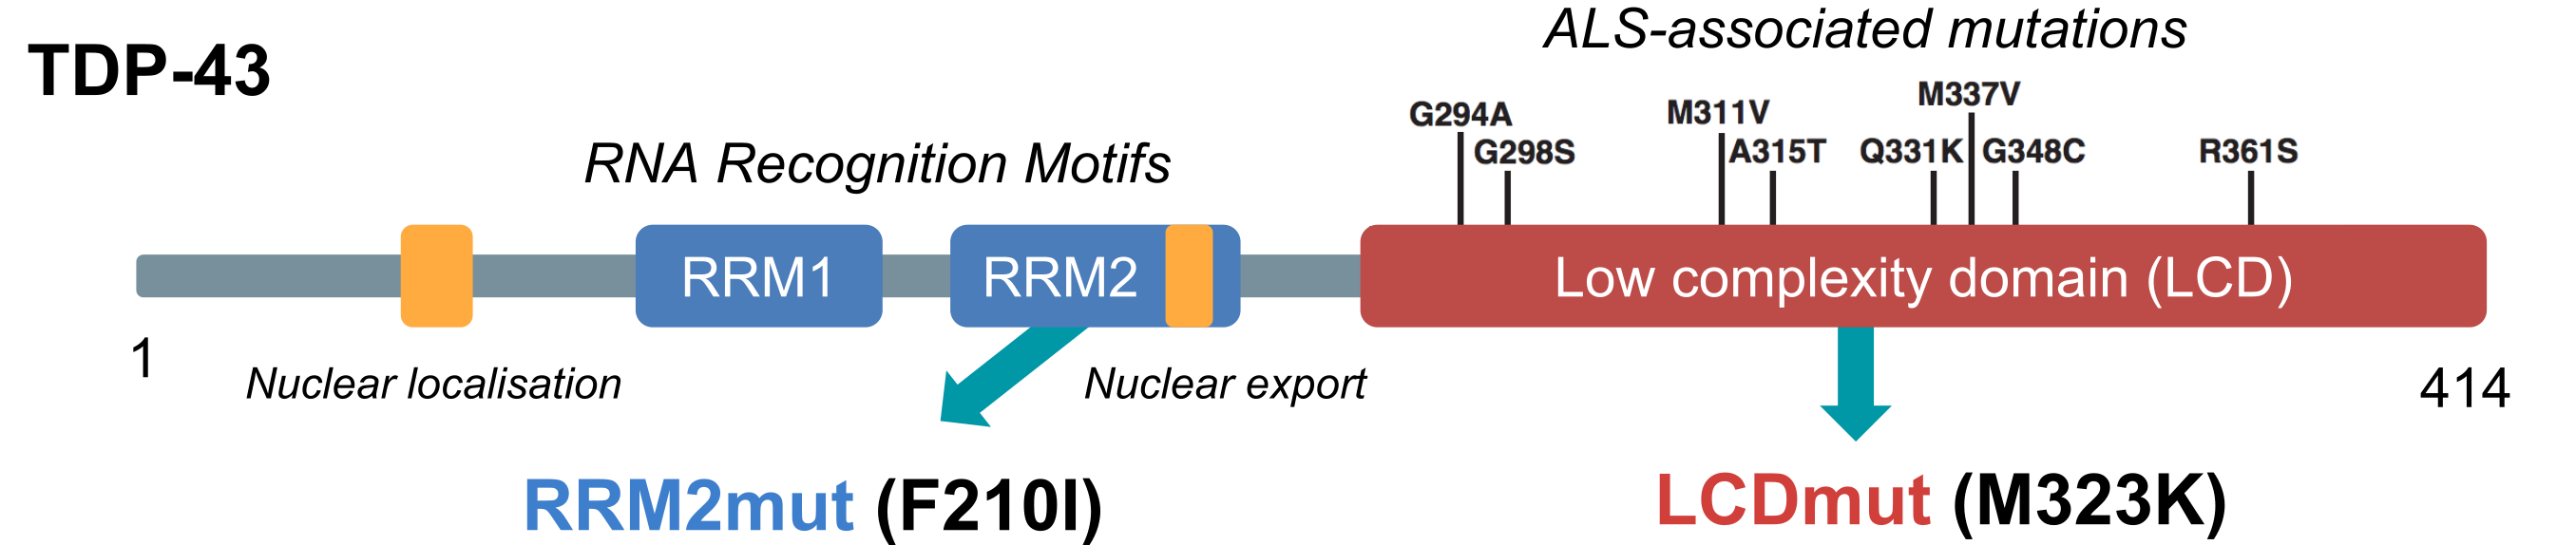
\includegraphics[width=\textwidth]{Figures/05_tdp_mice/TDP_structure_mutations.png}
	\caption[The two TARDBP mutations and their location within the TDP-43 protein]{
		\textbf{The two TARDBP mutations and their location within the TDP-43 protein.}
		RRM2mut affects the second RNA recognition motif whereas LCDmut affects the C-terminal low complexity domain.
	}
	\label{fig:tdp_structure}
\end{figure}

N-ethyl-N-nitrosourea (ENU) is a very potent mutagenic compound. Dosing male mice with ENU induces point mutations in sperm cells \citep{DeAngelis2000}. 
Large banks of mutant mouse sperm are maintained at MRC Harwell \citep{Acevedo2008} and the RIKEN in Japan \citep{Gondo2010}. 
From these resources two mouse lines with mutations in \textit{Tardbp} were chosen, F210I and M323K. 
The F210I mutation lies within the second RNA recognition motif (RRM2) of the TDP-43 protein whereas M323K lies within the C-terminal low complexity domain (LCD). 
This region is a hotspot for ALS mutations (Fig. \ref{fig:tdp_structure}). 
The M323K mutation lies within a 20 amino acid alpha-helical region previously found to be important for liquid phase separation and protein aggregation \citep{Conicella2016}. 
Developing these two mice allowed us to interrogate TDP-43 function and compare a mutation that would be predicted to impair the RNA binding ability of TDP-43 (F210I) with a mutation that potential resembles ALS (M323K). 
Due to their positions within the protein, the two mutations will be henceforth referred to as RRM2mut and LCDmut.

% info on breeding - F210I is embryonic lethal
We derived mice from mutant sperm and backcrossed for 10 generations onto a mixed C57BL/6J - DBA/2J background to remove unwanted background mutations.
RRM2mut is embryonic lethal in the homozygous state but not in heterozygosity, whereas homozygous LCDmut mice are viable and live normal lifespans. 
The two mutant lines were crossed together to create compound heterozygotes.
The RRM2mut/LCDmut mice were viable, suggesting the two mutations complement each other.
Close observation of aged LCDmut revealed gradual muscle weakness and a reduction in motor neuron numbers in the spinal cord (data not shown), suggesting that the patient-like M323K mutation indeed causes symptoms of neurodegeneration reminiscent of ALS. 
Due to the extreme differences in phenotype, particularly the neurodegeneration seen in LCDmut adults, I was curious to explore the effect of the mutations on RNA splicing.

\subsection{The two mutations have opposing effects on splicing known TDP-43 targets}

\begin{figure}[h!]
	\centering
	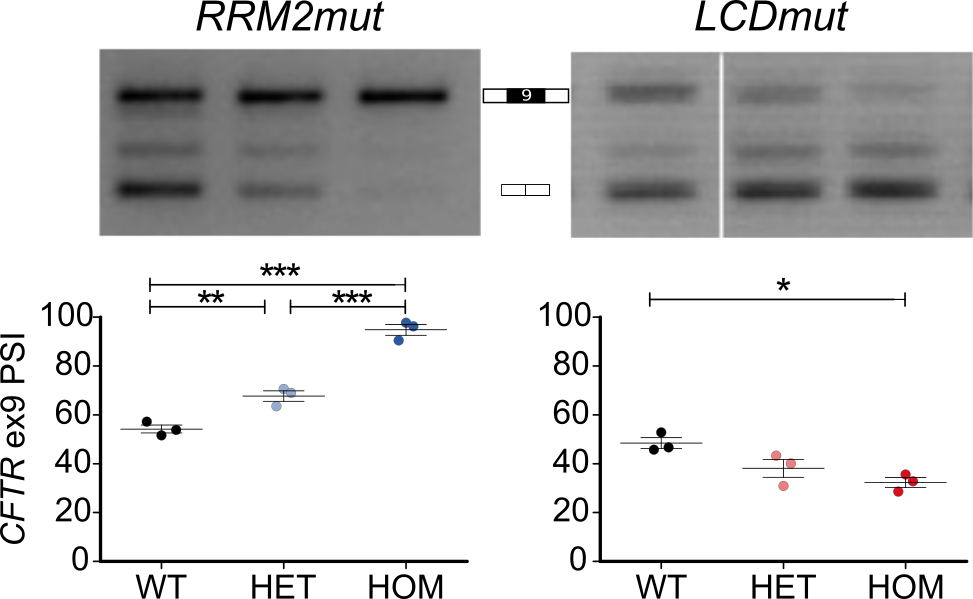
\includegraphics[width=10cm]{Figures/05_tdp_mice/CFTR.png}
	\caption[Opposite effects on splicing CFTR exon 9 minigene, a known TDP-43 splicing target]{
		\textbf{Opposite effects on splicing CFTR exon 9 minigene, a known TDP-43 splicing target.}
	RT-PCR traces from primers flanking CFTR exon 9, quantified as PSI ratios for each genotype. *** P < 0.0001 (ANOVA); ** P < 0.01; *** P < 0.001 (Tukey post-hoc test).
	}	
	\label{fig:CFTR}
\end{figure}

Exon 9 of the \textit{CFTR} gene was the first mRNA splicing target of TDP-43 to be described in the literature \citep{Buratti2001-et}. Knocking down TDP-43 leads to increased exon 9 inclusion, suggesting that TDP-43 acts to promote exon skipping. 
We made use of a minigene construct created from \textit{CFTR} exon 9 and its two flanking introns and exons \citep{Buratti2007minigene}.
Reverse-Transcriptase Polymerase Chain Reaction (RT-PCR) was performed to amplify between primers that flank exon 9. 
Analysis of the gel electrophoresis traces shows two primary bands: a larger band corresponding to exon 9 inclusion and a smaller band corresponding to exon 9 skipping. 
RRM2mut has a clear dose-dependent increase in exon 9 inclusion compared to skipping and thus resembles a loss of TDP-43 splicing function (Fig.  \ref{fig:CFTR}). 
Conversely, LCDmut has a dose-dependent increase in exon 9 skipping.
This suggests that the pro-skipping action of TDP-43 is increased at the CFTR locus and the LCDmut mutation causes a gain of splicing function.

%% INSERT TDP MEF SCATTERS
\begin{figure}[h]
	\centering
	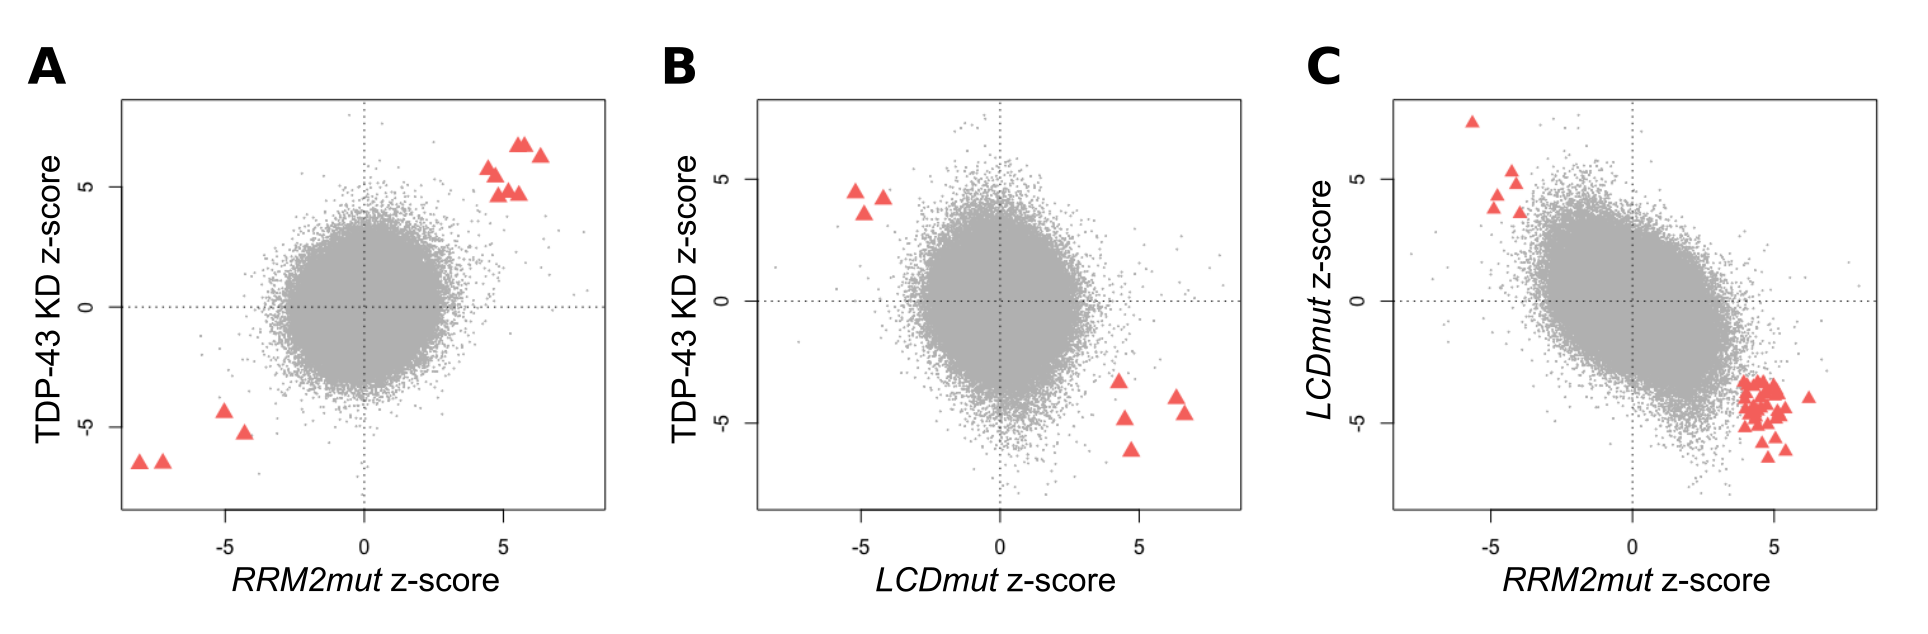
\includegraphics[width=\textwidth]{Figures/05_tdp_mice/mef_scatters.png}
	\caption[Comparing exon usage between the two mutations and a TDP-43 knockdown]{
		\textbf{Comparing exon usage between the two mutations and a TDP-43 knockdown.}
	Signed Z-scores for all exons found by DEXSeq in the mouse embryonic fibroblasts, comparing a TDP-43 shRNA knockdown to RRM2mut \textbf{(A)} and LCDmut \textbf{(B)} and comparing the two mutations \textbf{(C)}. Exons significant at FDR < 10\% plotted as red triangles, non-significant exons plotted as grey dots.
}
	\label{fig:mef_scatters}
\end{figure}

To look transcriptome-wide at the effects of the two mutations on simple cassette exon splicing the lab generated low-depth RNA-seq data from mouse embryonic fibroblasts. 
To compare both mutations to a simple loss of TDP-43 a short hairpin RNA (shRNA) was designed to be complementary to \textit{Tardbp} mRNA.
Binding of the shRNA should target \textit{Tardbp} mRNA for degradation, reducing TDP-43 protein levels. 
I performed a cassette exon splicing analysis and converted the fold change and \textit{P}-value from each exon into a signed Z-score. 
This allows for two way comparisons  between the shRNA knockdown of TDP-43 (TDP-KD), LCDmut and RRM2mut. 
Separating each graph into quadrants makes it clear that all significantly changed exons found in each mutation are changed in the same direction between RRM2mut and TDP-KD (Fig. \ref{fig:mef_scatters}). 
However, the exon changes are opposing when comparing LCDmut and TDP-KD, as well as between LCDmut and RRM2mut . 
This provides evidence at transcriptome scale that RRM2mut is a loss of splicing function whereas LCDmut is behaving oppositely.

%%CASSETTE EXON SCATTERS
\begin{figure}[h]
	\centering
	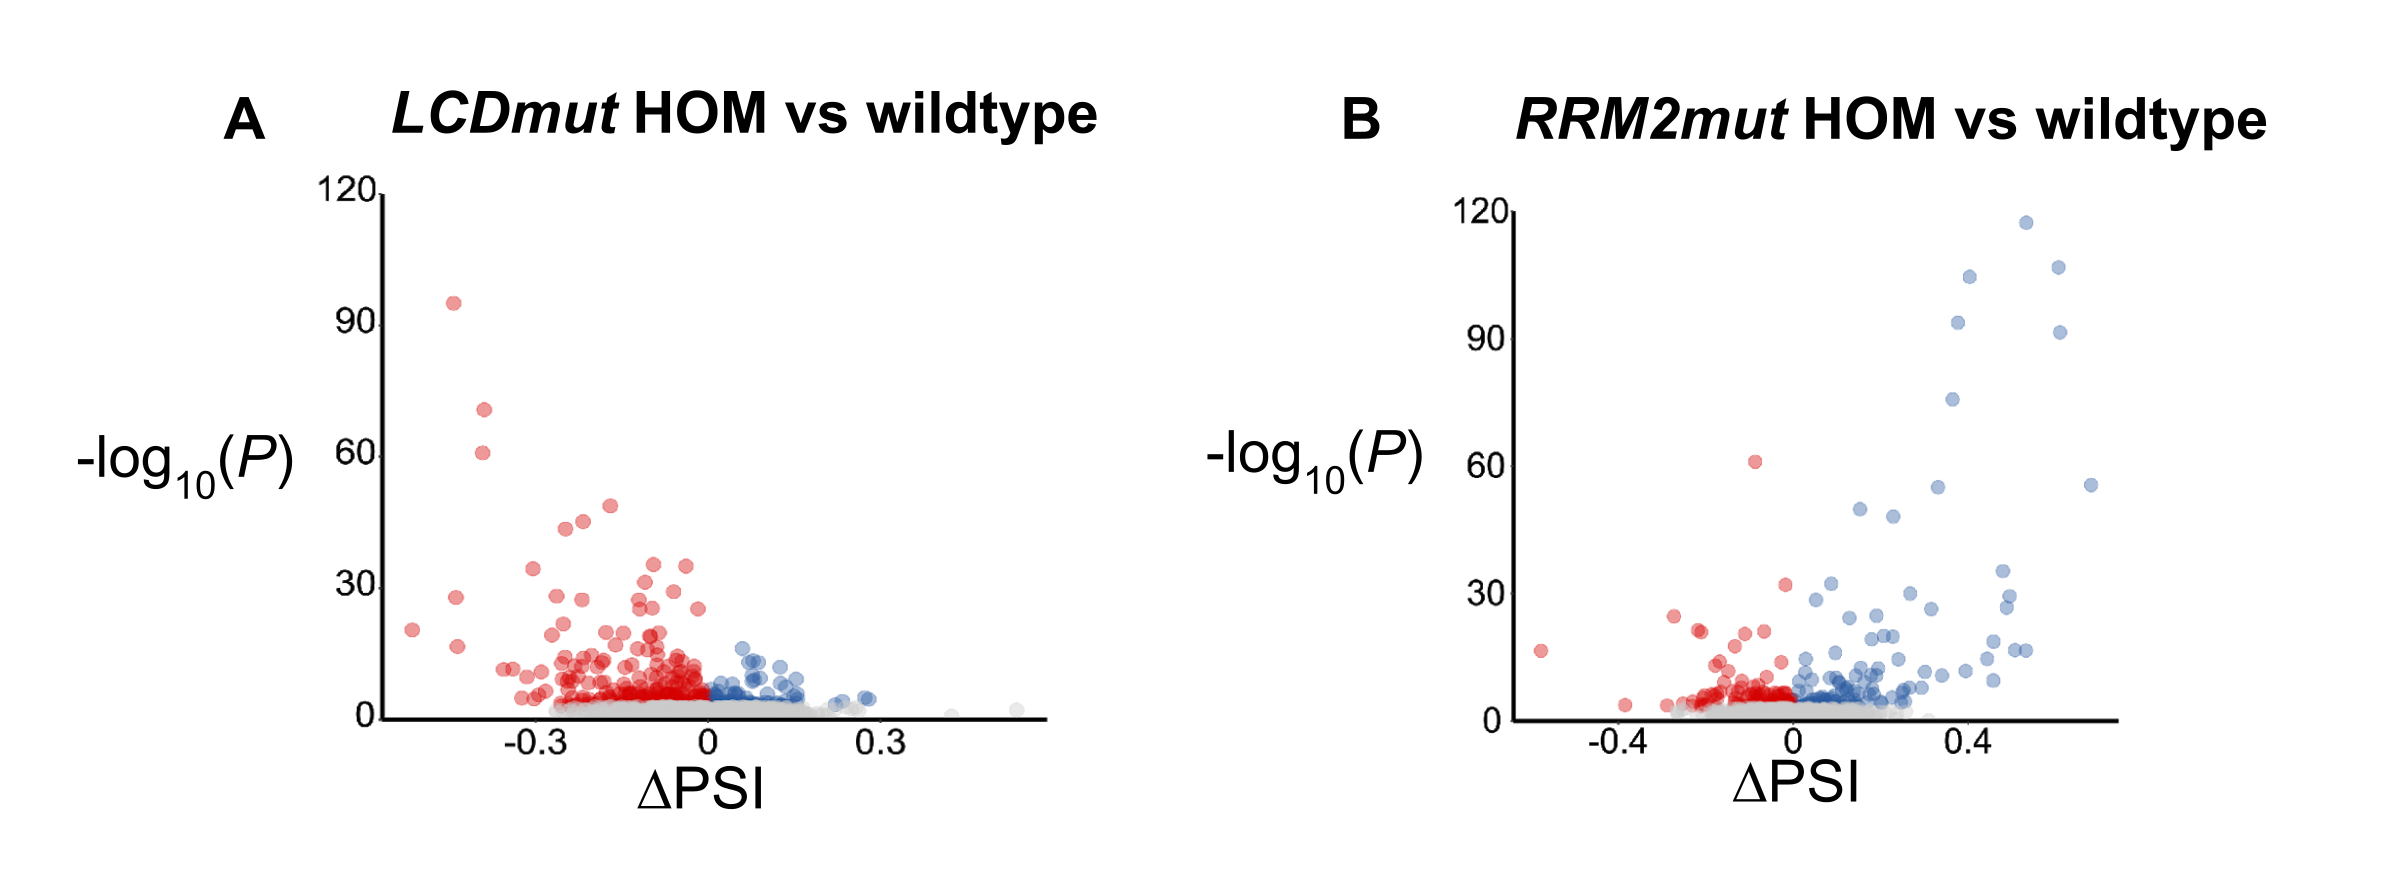
\includegraphics[width=\textwidth]{Figures/05_tdp_mice/transcriptome_scatters.png}
	\caption[Direction of cassette exon splicing in the two mutant lines]{
		\textbf{Direction of cassette exon splicing in the two mutant lines.}
	All splicing events found by SGSeq plotted by \textit{P}-value and direction ($\Delta$PSI; see methods) for LCDmut \textbf{(A)} and RRM2mut \textbf{(B)}.
}
	\label{fig:cassette_scatters}
\end{figure}

To deeply interrogate splicing changes at time points that were relevant to the phenotypes of interest (death in RRM2mut and neurodegeneration in LCDmut) high depth RNA-seq data was generated from RRM2mut embryonic brains and LCDmut adult brains (30 days post-natal). 
Higher depth and longer read data allows for better discrimination of novel splicing events and so I ran a novel splicing analysis using SGSeq \citep{Goldstein2016}. 
Plotting the direction and \textit{P}-value of all cassette exons found in the two mutations strongly suggests that the strongest splicing changes are in exon inclusion in RRM2mut and in exon skipping in LCDmut (Fig. \ref{fig:cassette_scatters}).

% RNAmaps of the cassettes - motif and iCLIP
\begin{figure}[h]
	\centering
	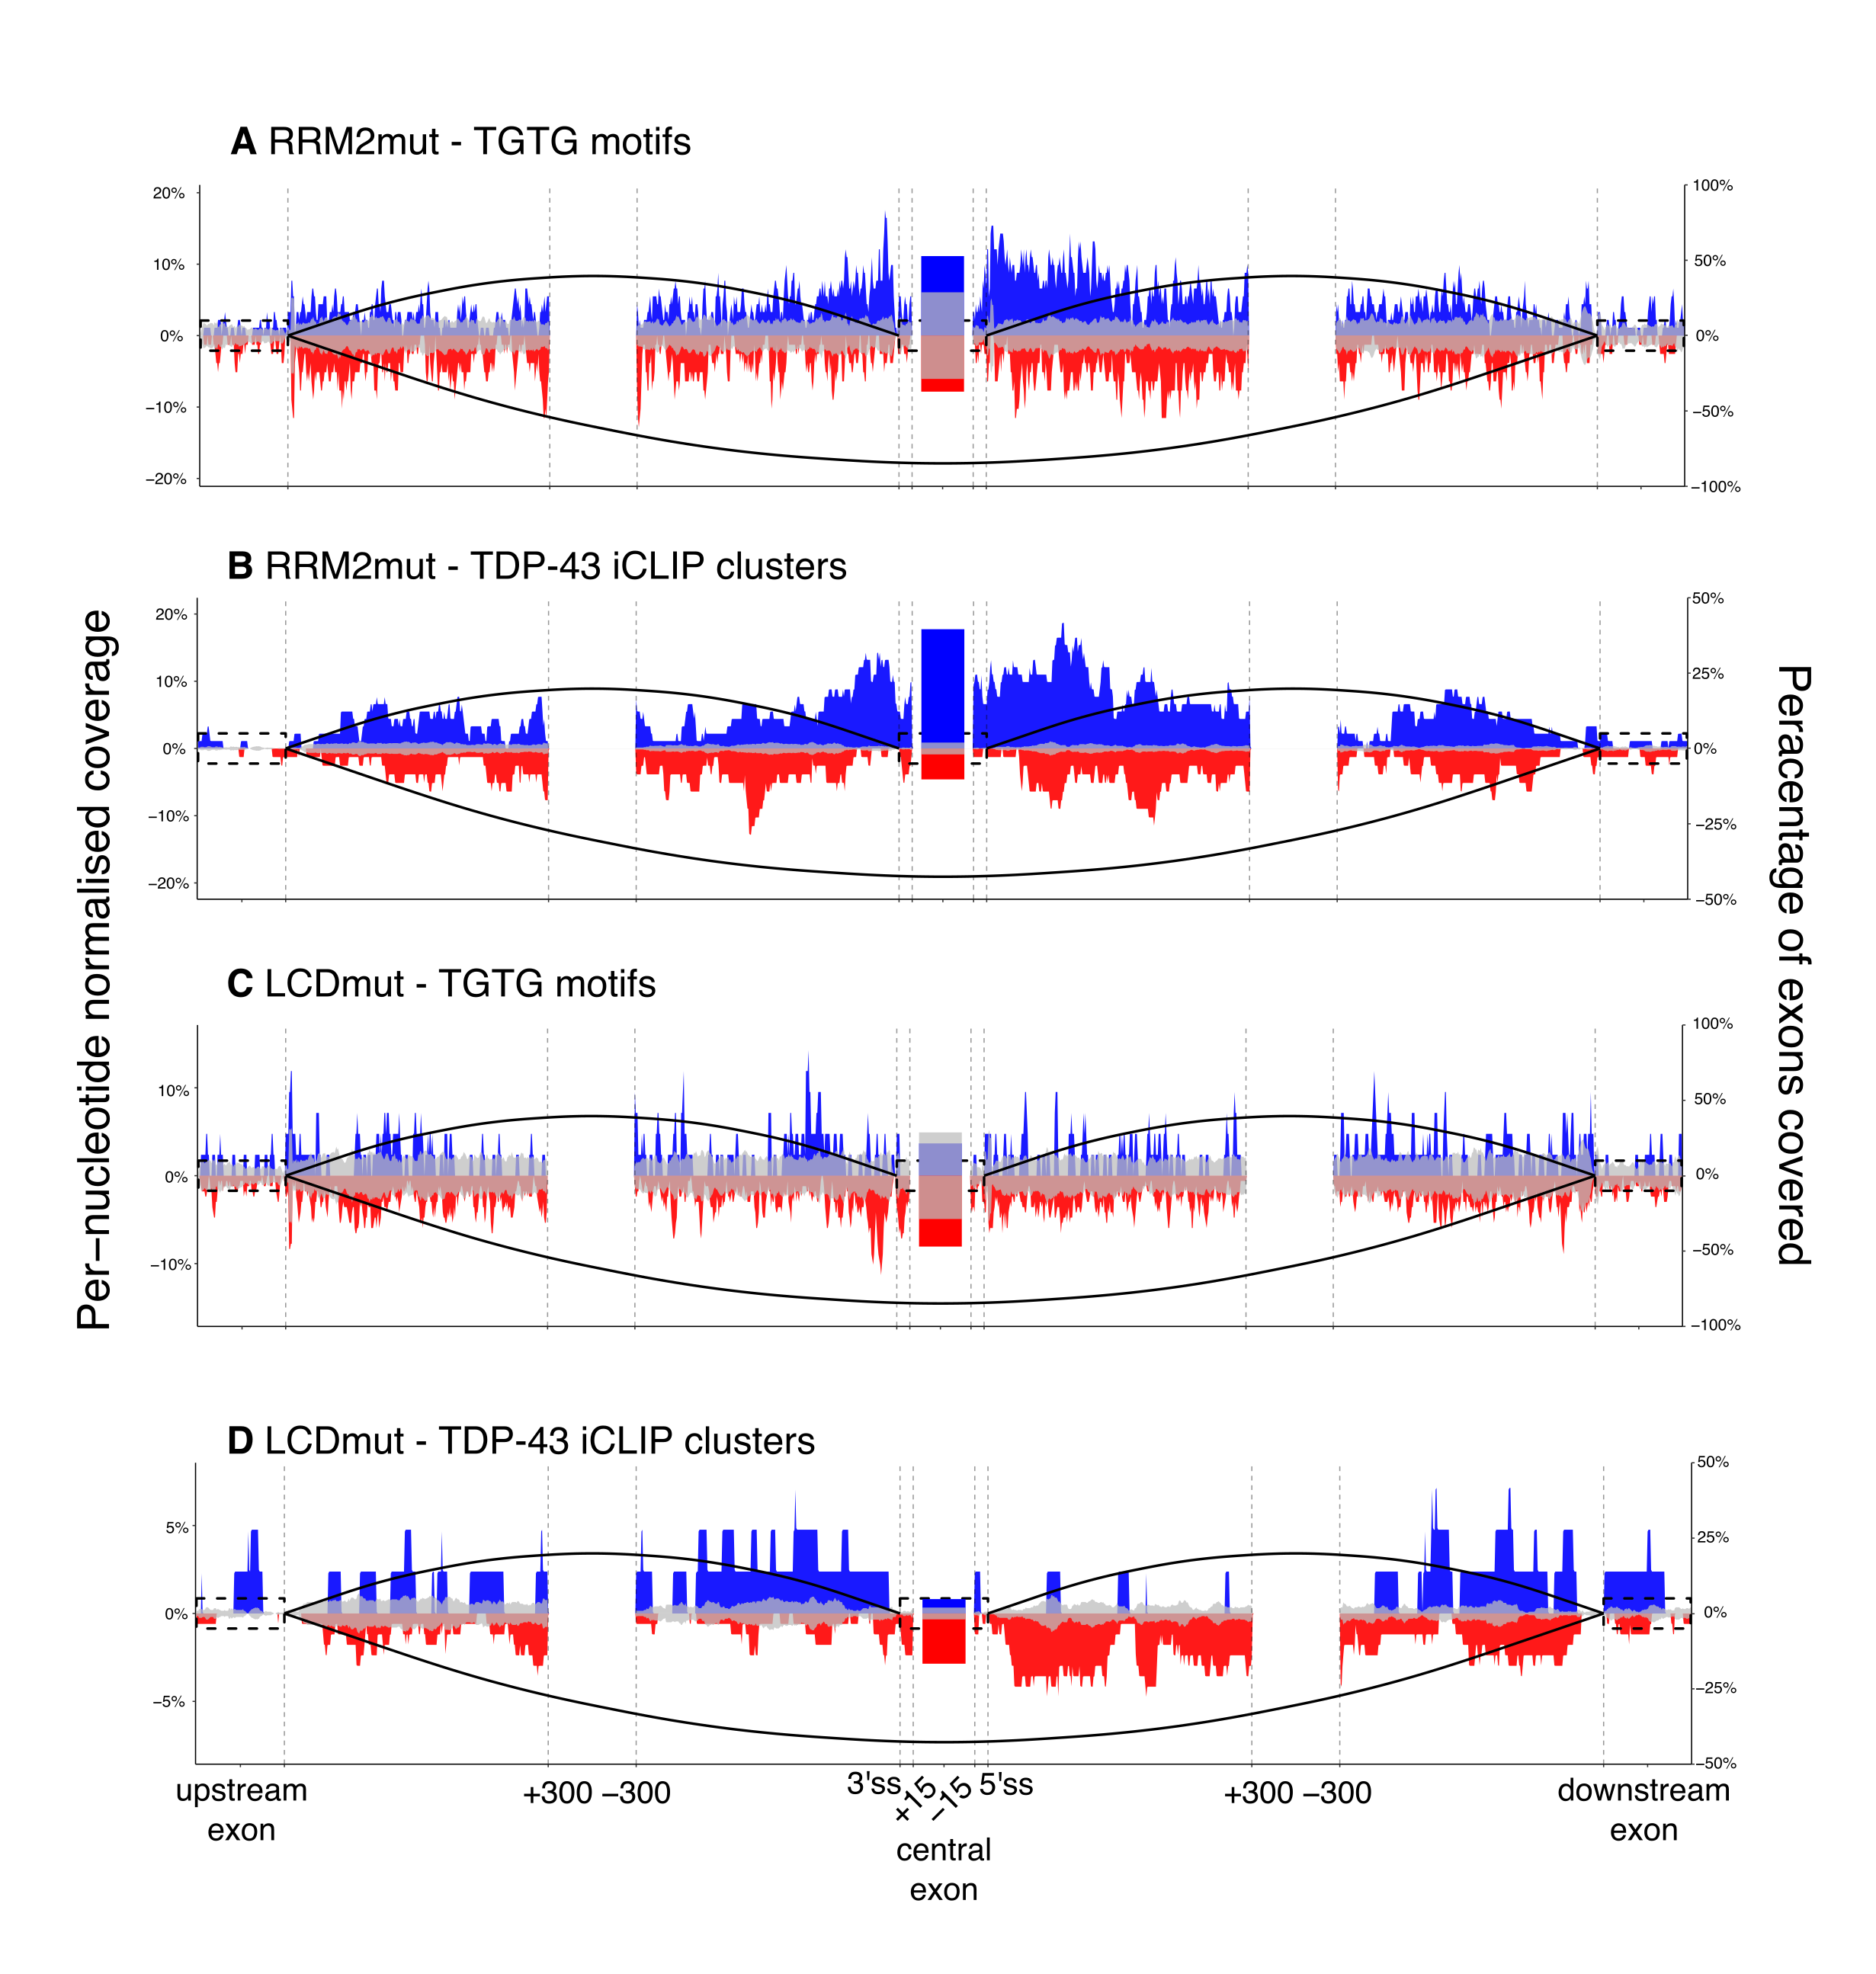
\includegraphics[width=14cm]{Figures/05_tdp_mice/RNAmap_cassettes.png}
	\caption[RNA maps visualise positional enrichment of iCLIP and sequence motifs]{
		\textbf{RNA maps visualise positional enrichment of iCLIP and sequence motifs within cassette exon splicing loci.}
	RNA maps constructed from differentially included (blue) and skipped (red) cassette exons.  
	\textbf{(A)} TGTG motifs in RRM2mut.
	\textbf{(B)} TDP-43 iCLIP in RRM2mut.
	\textbf{(C)} TGTG motifs in LCDmut; 
	\textbf{(D)} TDP-43 iCLIP in RRM2mut.
	}
	\label{fig:RNAmap_cassettes}
\end{figure}

The splice-site competition model of cassette exon splicing allow an RNA-binding protein to either repress or enhance cassette exon splicing depending on the position it binds within the intron. When RNA binding proteins bind on top of or close to an exon, the recognition of that exon's splice sites by the spliceosome is blocked and the exon is no longer included in a transcript. Conversely, if an RNA binding protein binds deeper within the intron it can act to recruit the spliceosome to the exon and enhance exon inclusion. 
% CITATIONS - PTBP, NOVA etc
I created RNA maps to look for positional enrichment within and around the the cassette exons, both for UGUG sequence motifs as well as RNA-protein interaction information from iCLIP experiments. For each set of exons I used a random set of 1994 cassette exons which were not significantly changed as a null distritbution.
Motif-based maps were calibrated using the invariant AG and GT dinucleotides at the 3' and 5' splice sites respectively (see appendices).
For RRM2mut, the 91 cassette exons with increased inclusion were enriched in UGUG sequence motifs (Fig \ref{fig:RNAmap_cassettes}A) and iCLIP peaks (Fig \ref{fig:RNAmap_cassettes}B).
Both sequence features either directly overlap the exon or are within 100 bp either side. 
The 78 skipped exons  in RRM2mut were depleted in both feature types directly on top and close by. 
LCDmut cassette exons show the inverse distribution to RRM2mut as the 168 skipped exons are enriched for features that directly overlap and closely flank the exons (Fig \ref{fig:RNAmap_cassettes}C/D), whereas the 42 included exons were depleted of sequence features that were close or overlapping.
All exons howed enrichment of TDP-43 features at the distal flanking 5' and 3' splice sites, suggesting long range cooperation around the distal splice sites.
This data suggests that whereas the RRM2mut cassette exons are shifted due to a reduction in TDP-43, the LCDmut exons are shifting in a direction suggesting an increase of TDP-43 in the mutant cells.

% include numbers!
%RNAmaps
%RRM2mut casssette exons: included 91, skipped 78, control 1994
%LCDmut cassette exons:  42, 168, 1994


\subsection{RRM2mut leads to a loss of splicing function and cryptic exons}

%% CRYPTIC EXONS IN RRM2mut
\begin{figure}[h!]
	\centering
	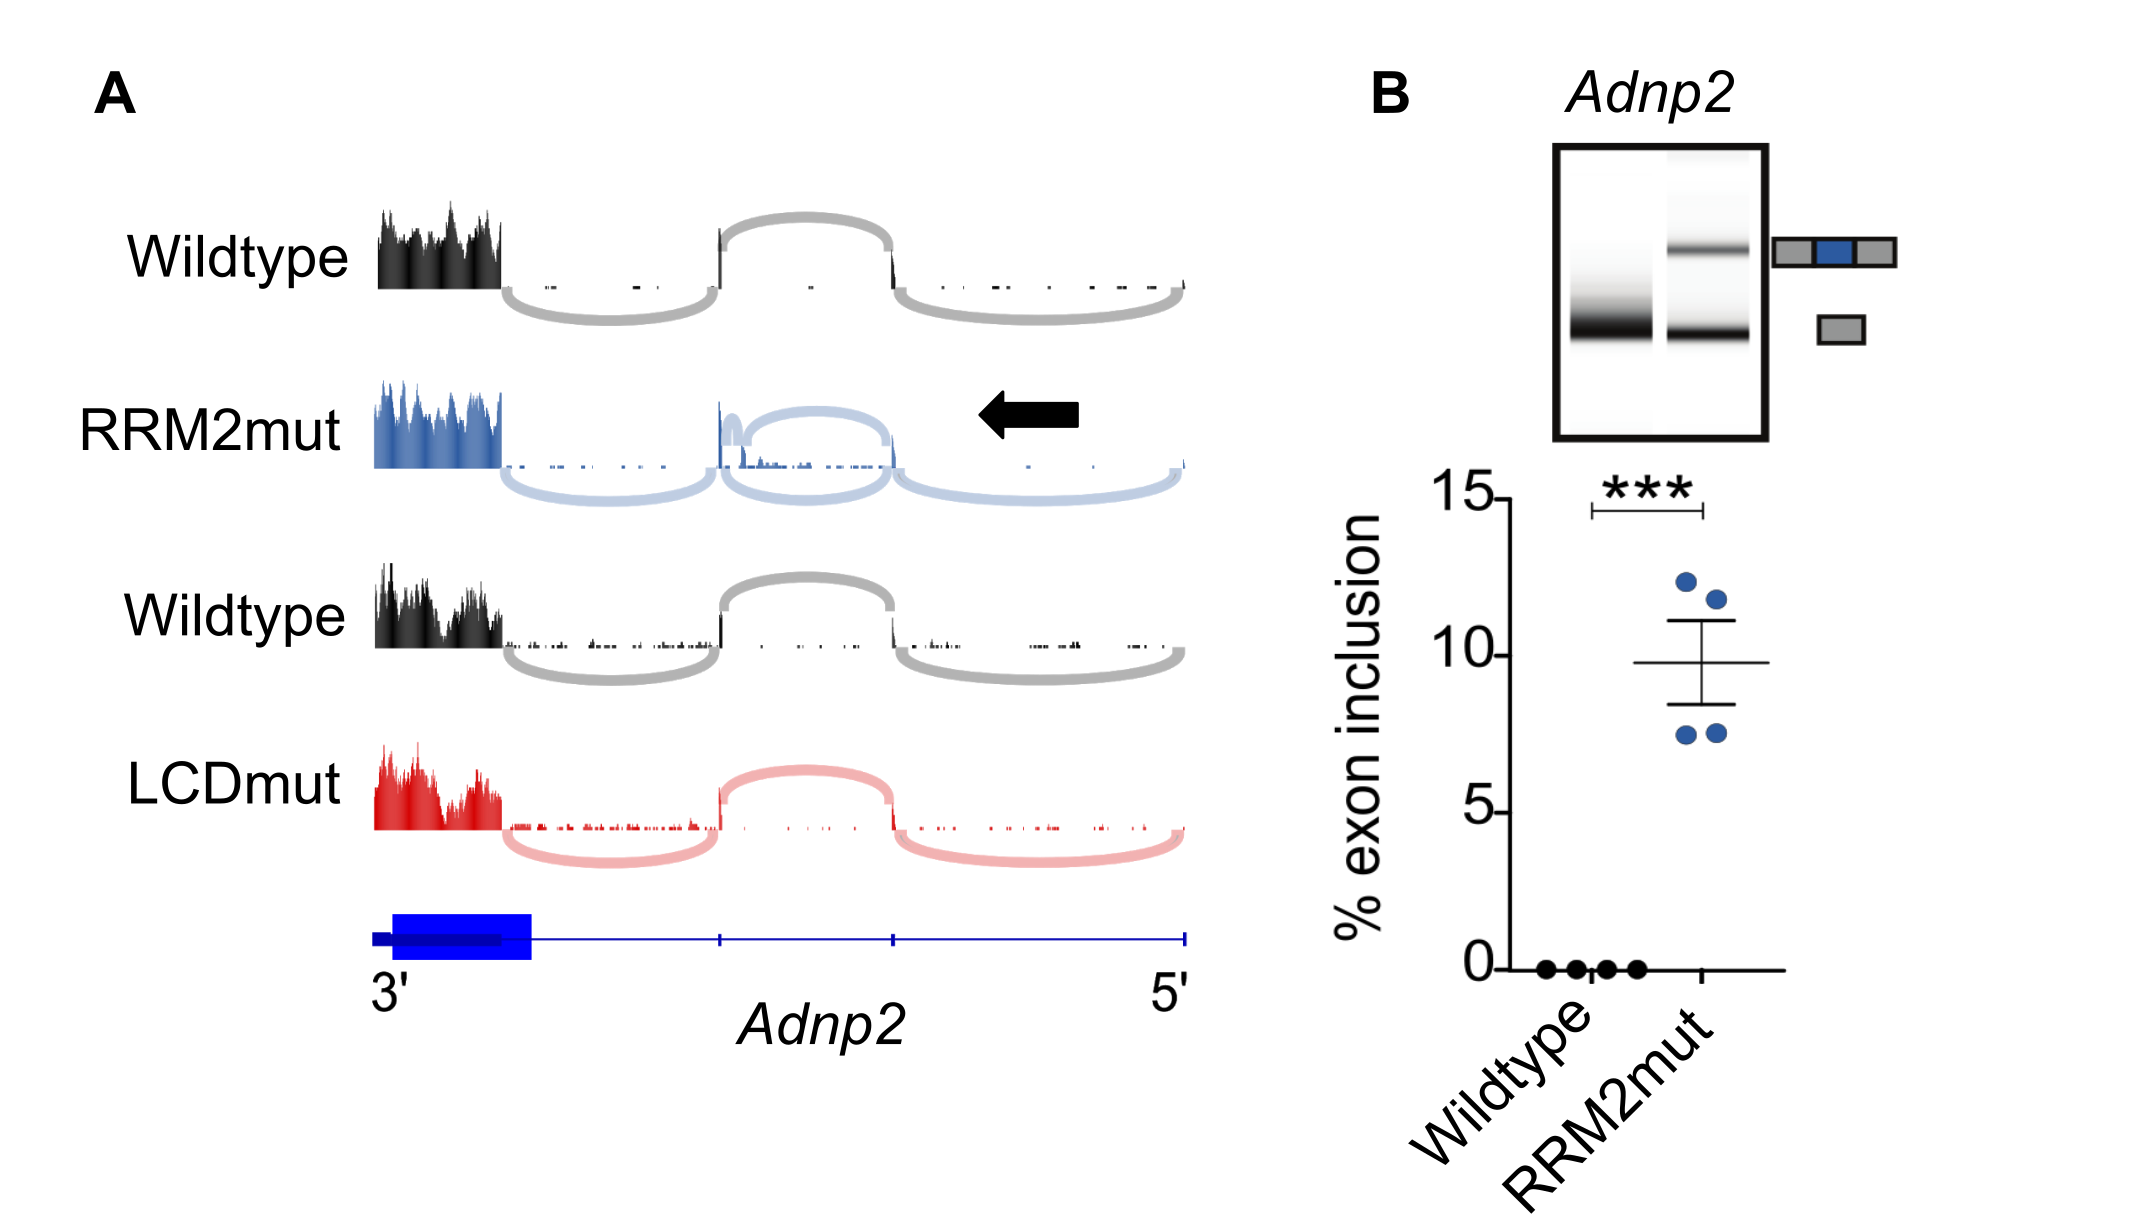
\includegraphics[width=14cm]{Figures/05_tdp_mice/cryptic_exon_multi.png}
	\caption[RRM2mut leads to cryptic exon splicing]{
		\textbf{RRM2mut leads to cryptic exon splicing.}
	\label{cryptic_multi}
	\textbf{(A)} Representative RNA-seq traces show cryptic exon in \textit{Adnp2} included in RRM2mut specifically. 
	\textbf{(B)} RT-PCR of \textit{Adnp2} selectively amplifies a band corresponding to cryptic exon inclusion in RRM2mut samples. P < 0.001; t-test(two-sided).
}
\end{figure}

A hallmark of TDP-43 depletion is the widespread inclusion of non-conserved cryptic exons \citep{Ling2015}. The bias towards cassette exon inclusion suggested that a number of RRM2mut repressed exons may be cryptic exons. Rather than relying on isoform annotation I filtered all cassette exons found in RRM2mut and selected those that were barely or not at all spliced in wildtypes but were included in RRM2mut samples, resulting in 33 candidate cryptic exons being discovered. A representative example of a cryptic exon in \textit{Adnp2} is shown in Fig. \ref{cryptic_multi}, changing from 0\% inclusion in wildtype mice to ~10\% inclusion in RRM2mut but not in LCDmut mice.  

%% LONG GENES 
\begin{figure}[h]
	\centering
	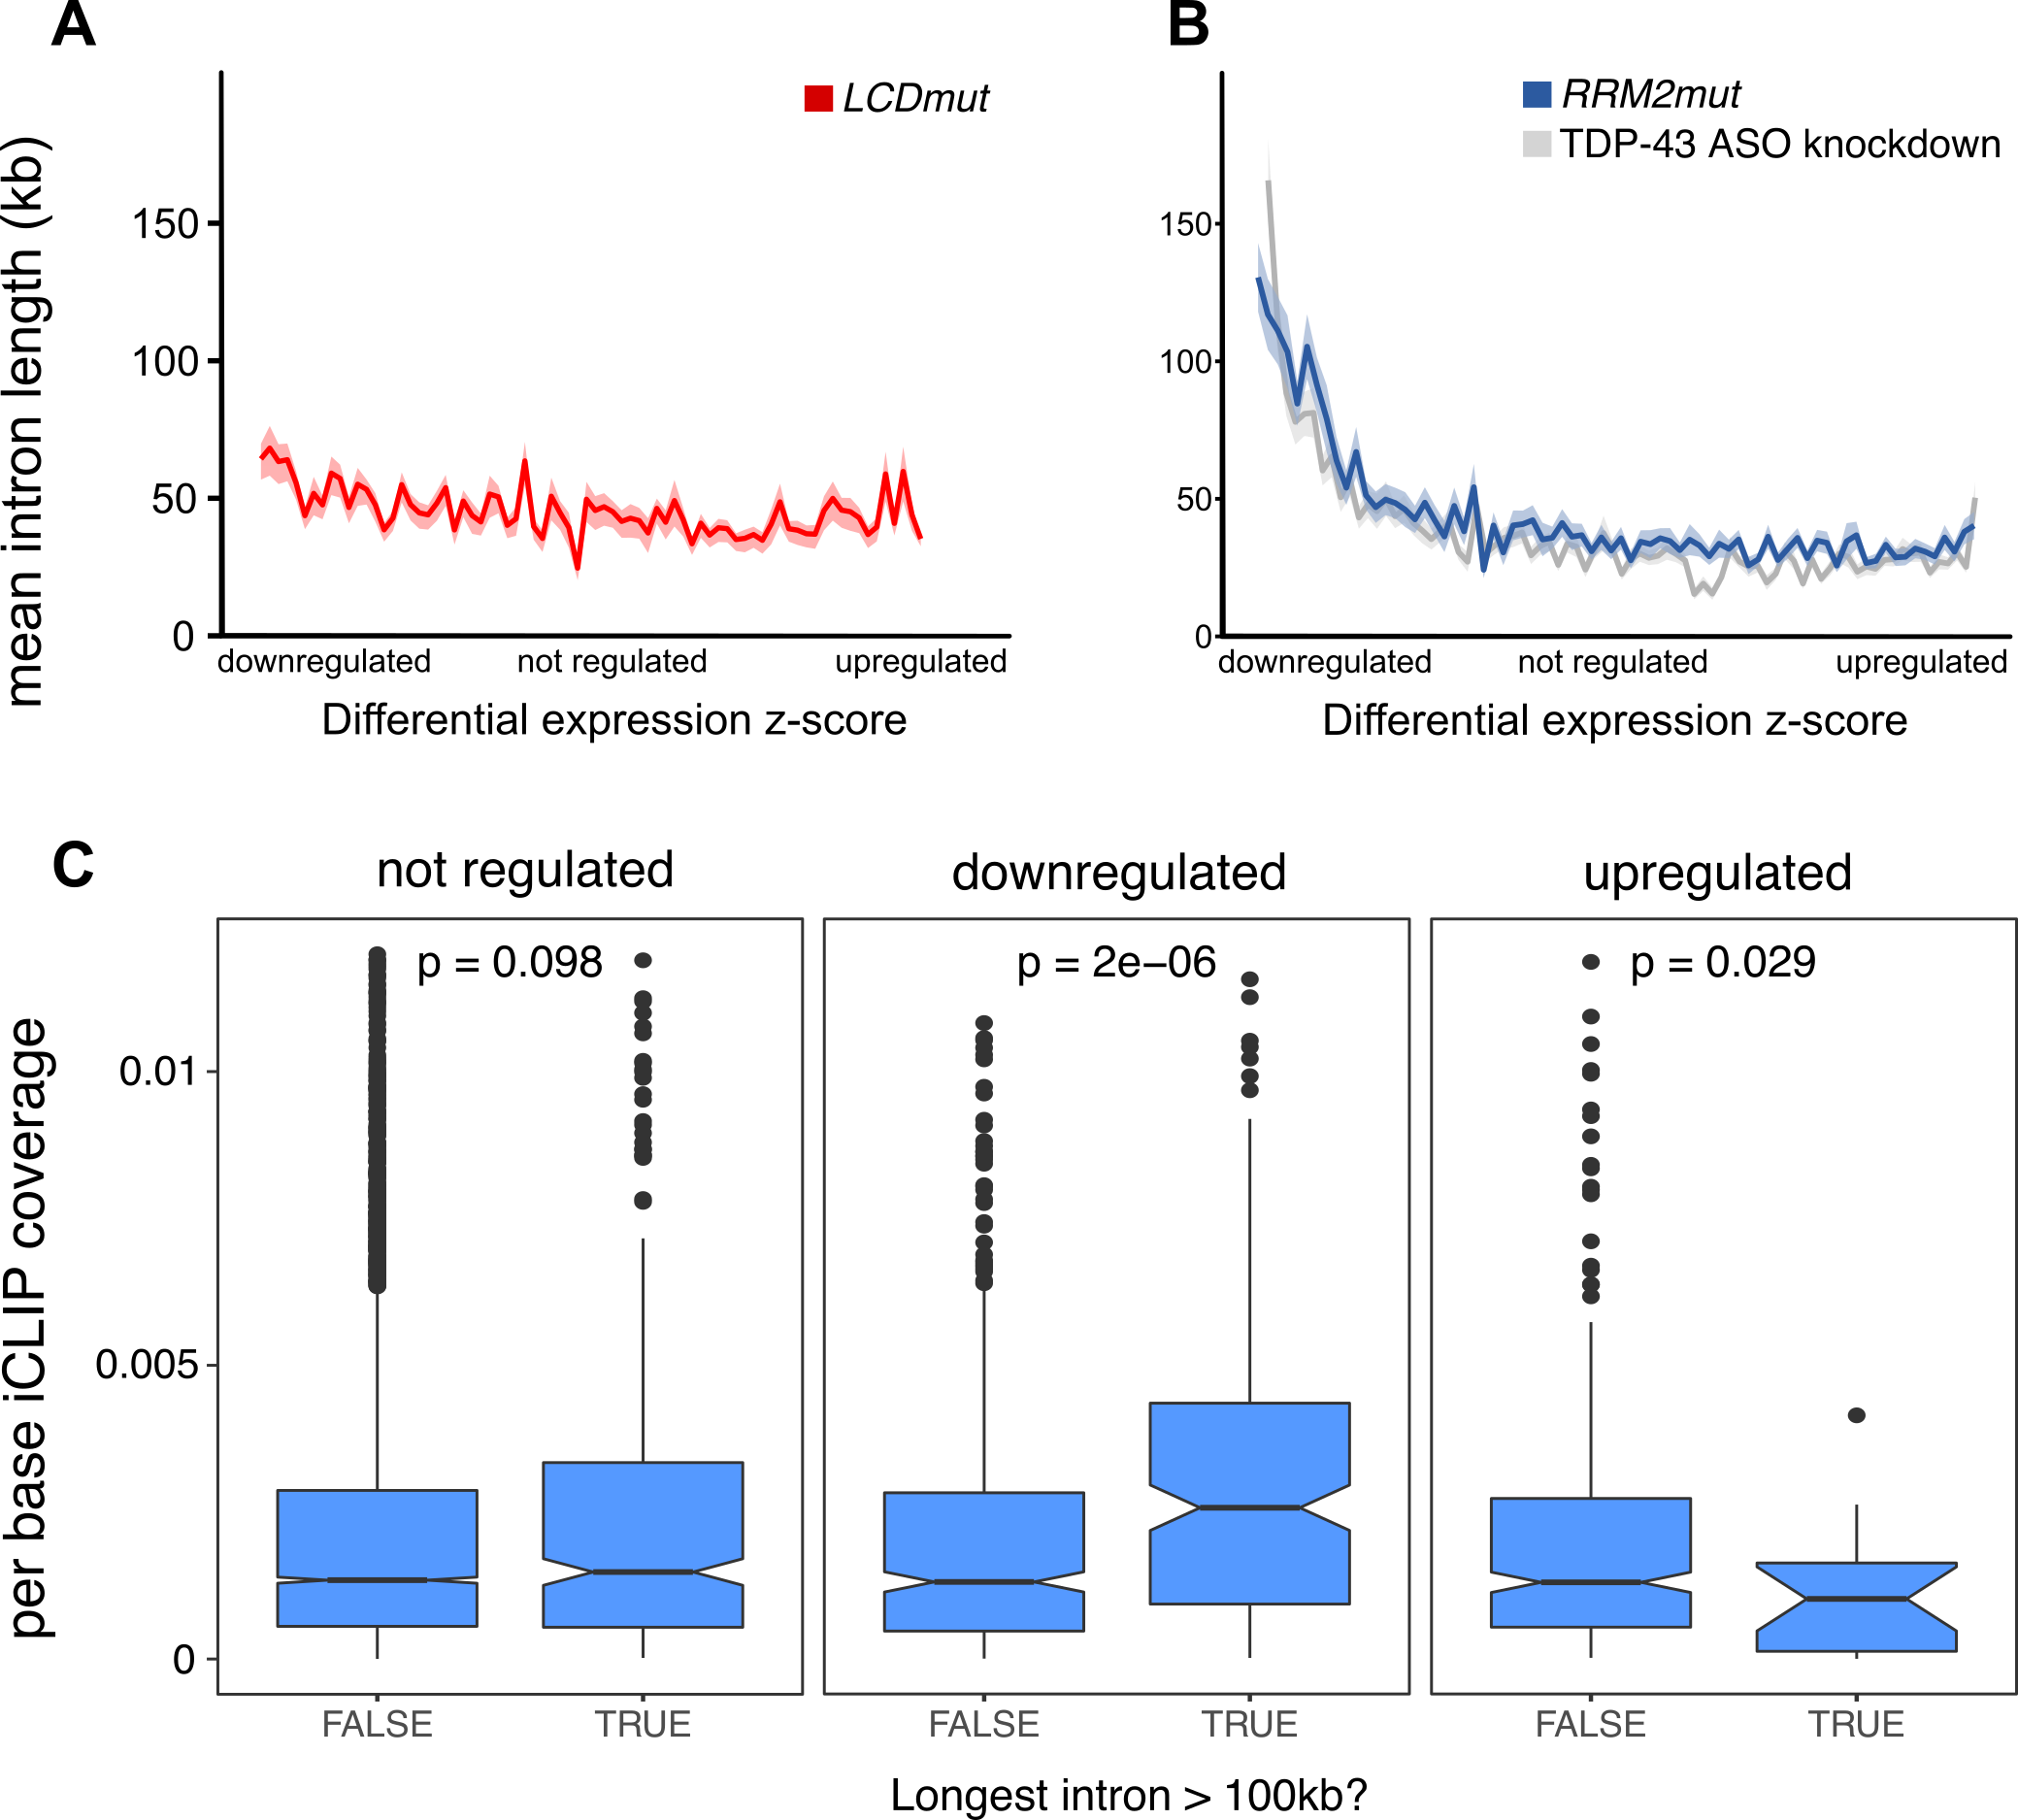
\includegraphics[width=12cm]{Figures/05_tdp_mice/long_genes_multi.png}
	\caption[RRM2mut gene expression has bias for long gene downregulation]{
		\textbf{RRM2mut gene expression has bias for long gene downregulation, mirroring TDP-43 knockdown data.}
	\textbf{(A,B)} Mean intron length in kilobases for bins of genes ordered by signed Z-score. TDP-43 antisense olignucleotide (ASO) knockdown data taken from \cite{Polymenidou2011-hs}. \textbf{(C)} The per-nucleotide overlap of iCLIP interaction peaks for each gene is significantly increased in long intron genes downregulated in RRM2mut mice compared to wildtype. \textit{P}-values are from Mann-Whitney-Wilcoxon test.
}
	\label{fig:long_genes}
\end{figure}

Another feature of TDP-43 loss of function is a striking downregulation of genes with long introns (>100kb). This phenomenon was first observed in mice where an antisense oligonucleotide strategy was used to lower TDP-43 in the striatum (TDP-ASO); \citep{Polymenidou2011-hs}. Long intron genes are over-represented in neuronal cells \citep{Sibley2015} and it is thought that TDP-43 binds within these long introns to promote their processing and splicing. I re-analysed RNA-seq data from this study and compared it to the RRM2mut and LCDmut sequencing data. I ran a differential gene expression analysis with DESeq2 and ranked all genes by their direction of expression change between controls and ASO treatment/mutations. I then binned genes into groups of 200 and extracted the lengths of longest intron in each gene from GENCODE annotation. While in LCDmut, gene length is evenly distributed between downregulated, unchanged and upregulated genes (Fig. \ref{fig:long_genes}A), there is a clear bias for the most downregulated genes having long introns in both RRM2mut and TDP-ASO (Fig. \ref{fig:long_genes}B). An orthogonal approach is to look at TDP-43 protein-RNA interaction data performed on wildtype cells with the iCLIP method \citep{Huppertz2014-ip}. I calculated the proportion of nucleotides in each gene that had an iCLIP peak overlapping, suggesting direct TDP-43 binding. Genes that were downregulated in RRM2mut had no difference in the distribution of iCLIP peak overlaps except for those downregulated genes that also contained at least one intron longer than 100 kilobases (\textit{P}=2e-6; Fig. \ref{fig:long_genes}C). Long intron genes were modestly depleted in iCLIP peaks when the genes were upregulated (\textit{P}=0.029).


\subsection{LCDmut shows the inverse of cryptic splicing - skiptic splicing}

\begin{figure}[h!]
	\centering
	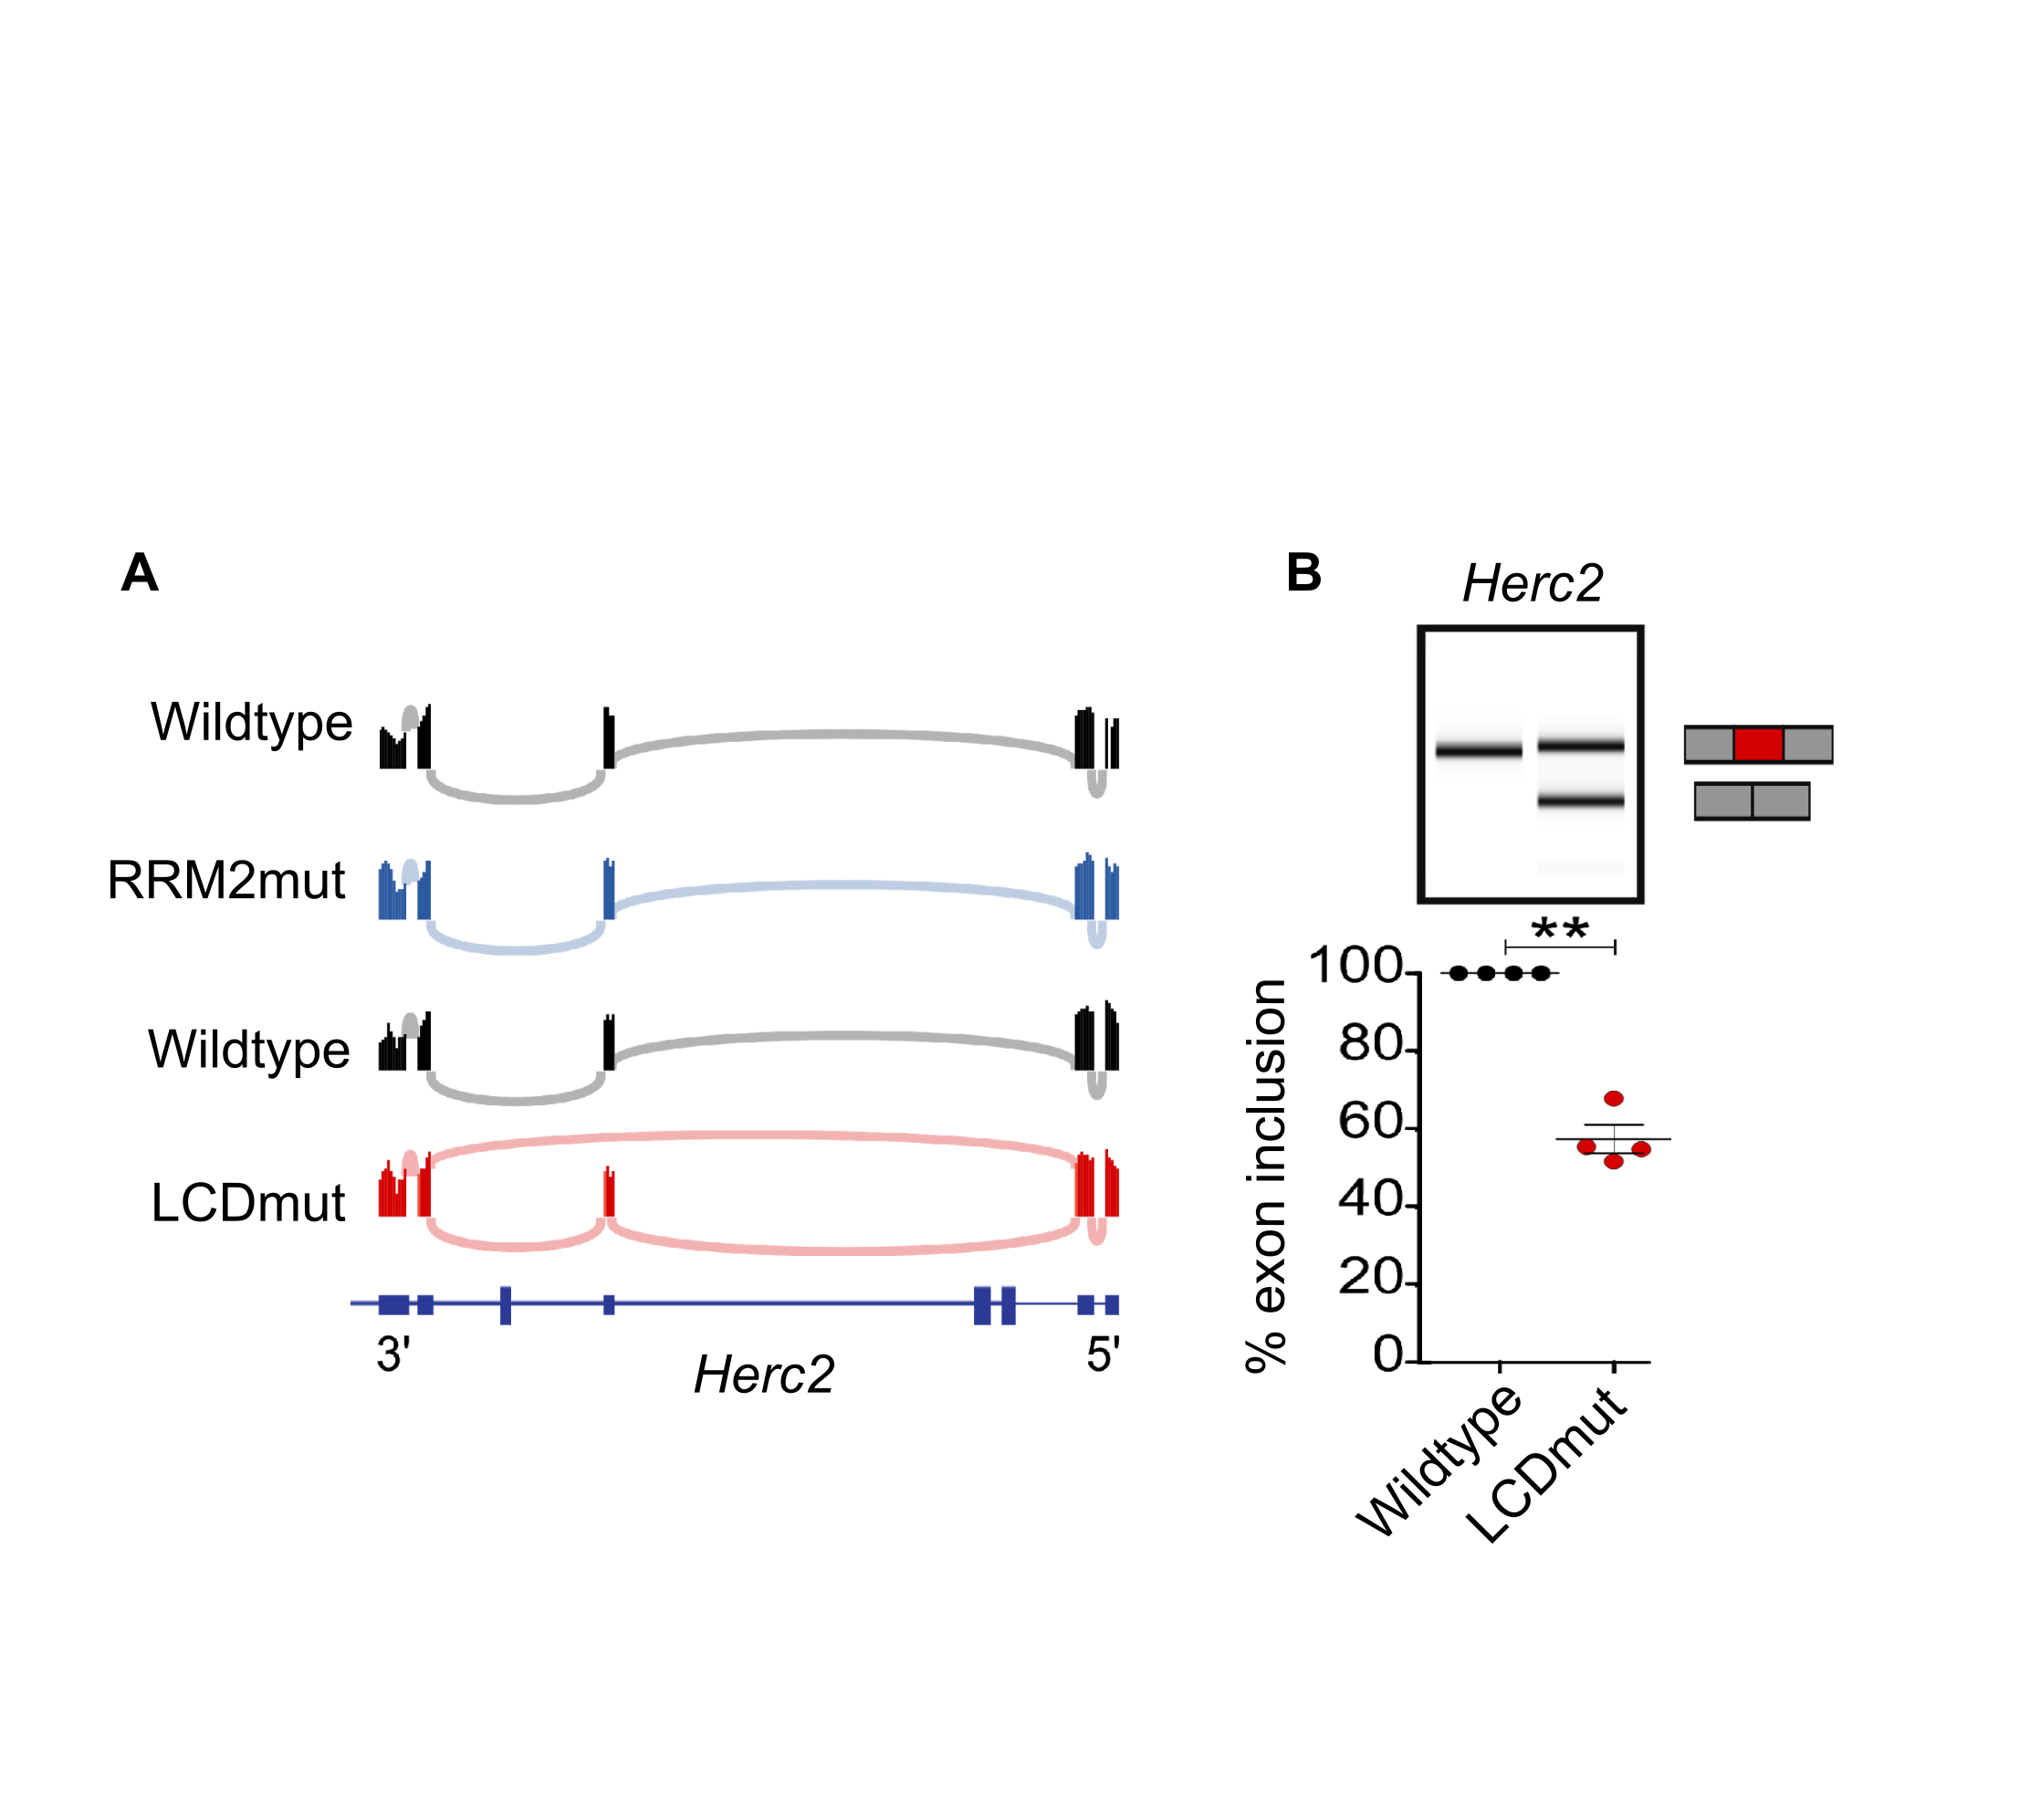
\includegraphics[width=12cm]{Figures/05_tdp_mice/skiptic_exon_multi.png}
	\caption[LCDmut leads to skiptic exon splicing]{
		\textbf{LCDmut leads to skiptic exon splicing.}
	\textbf{(A)} Representative RNA-seq traces show a constitutive exon in \textit{Herc2} skipped in LCDmut specifically - a skiptic exon. 
	\textbf{(B)} RT-PCR of \textit{Herc2} selectively amplifies a band corresponding to exon skipping skipping in LCDmut samples. P < 0.001; t-test(two-sided). 
	\textbf{(C)} PhyloP conservation scores for 1000 randomly chosen mouse exons compared to the 48 skiptic exons found in LCDmut.
}
	\label{fig:skiptic_multi}
\end{figure}

I applied the same cryptic exon filtering strategy to LCDmut and found a small number of potential cryptic exons. However, when applying the inverse critera to find exons that are 95-100\% included in wildtype and then skipped in LCDmut I uncovered 48 exons. These exons are constitutively spliced in wildtype samples and yet are skipped in LCDmut, making them the inverse of cryptic exons. I therefore christened them "skiptic" exons - a portmanteau of cryptic and skipping. A selection of skiptic exons were validated by RT-PCR (Fig. \ref{fig:skiptic_multi}). 


\begin{figure}[h!]
	\centering
	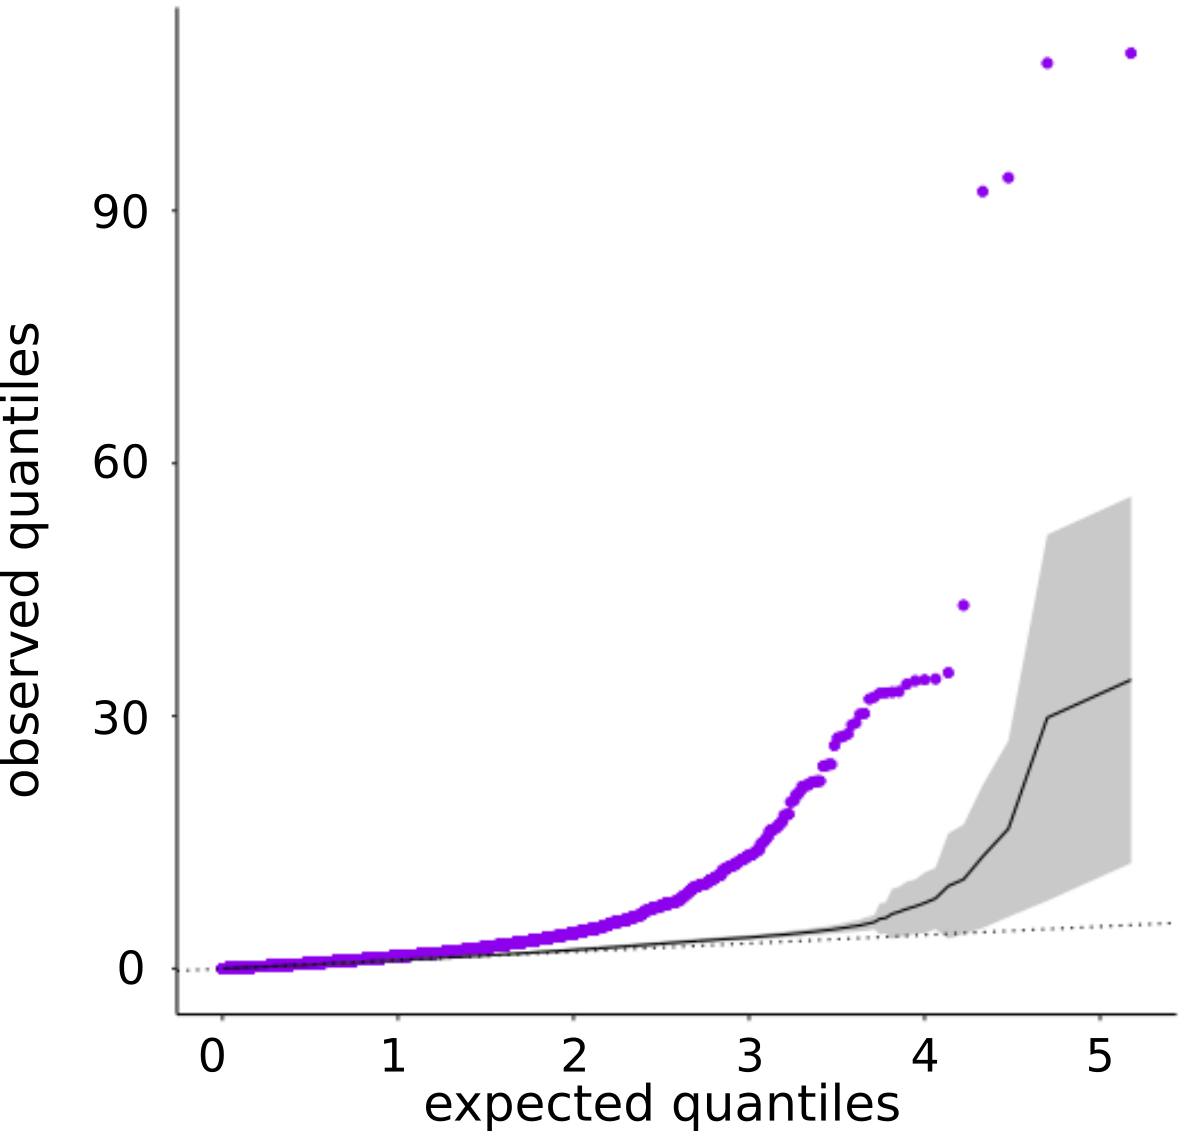
\includegraphics[width=7cm]{Figures/05_tdp_mice/permutation_ribbon.png}
	\caption[Permuting sample order shows clear splicing difference between LCDmut mice and controls]{
		\textbf{Permuting sample order shows clear splicing difference between LCDmut mice and controls.}
		Quantile-quantile plots show the difference between expected and observed distribution of \textit{P}-values generated from multiple tests. True case-control sample labelling of LCDmut and littermate controls (purple) shows clear inflation of low \textit{P}-values when compared to all permutations of sample ordering (grey; plotted as mean $\pm$ standard deviation).
	}
	\label{fig:permutation}
\end{figure}

To demonstrate that the 48 skiptic exons found in LCDmut were not statistical anomalies due to the small sample size I employed a permutation strategy.
 The wildtype and LCDmut labels were shuffled 50 times to cover all possible sample orders and the splicing analysis repeated with the permuted labels. 
A quantile-quantile plot contrasts the observed distribution of \textit{P}-values generated by a large number of statistical tests with the theoretical expected distribution. 
If there is no difference between genotypes then some low \textit{P}-values are expected by chance due to the small sample size and the large number of tests. 
However, there is a clear difference in splicing between LCDmut and wildtype mice that drives a large inflation in the number of low \textit{P}-value splicing events far away from the expected distribution (Fig. \ref{fig:permutation}).
A table of counts of all exons found at each permutation is presented in the appendices.   


\subsection{Both skiptic and cryptic splicing show evidence of direct TDP-43 binding}

\begin{figure}[h!]
	\centering
	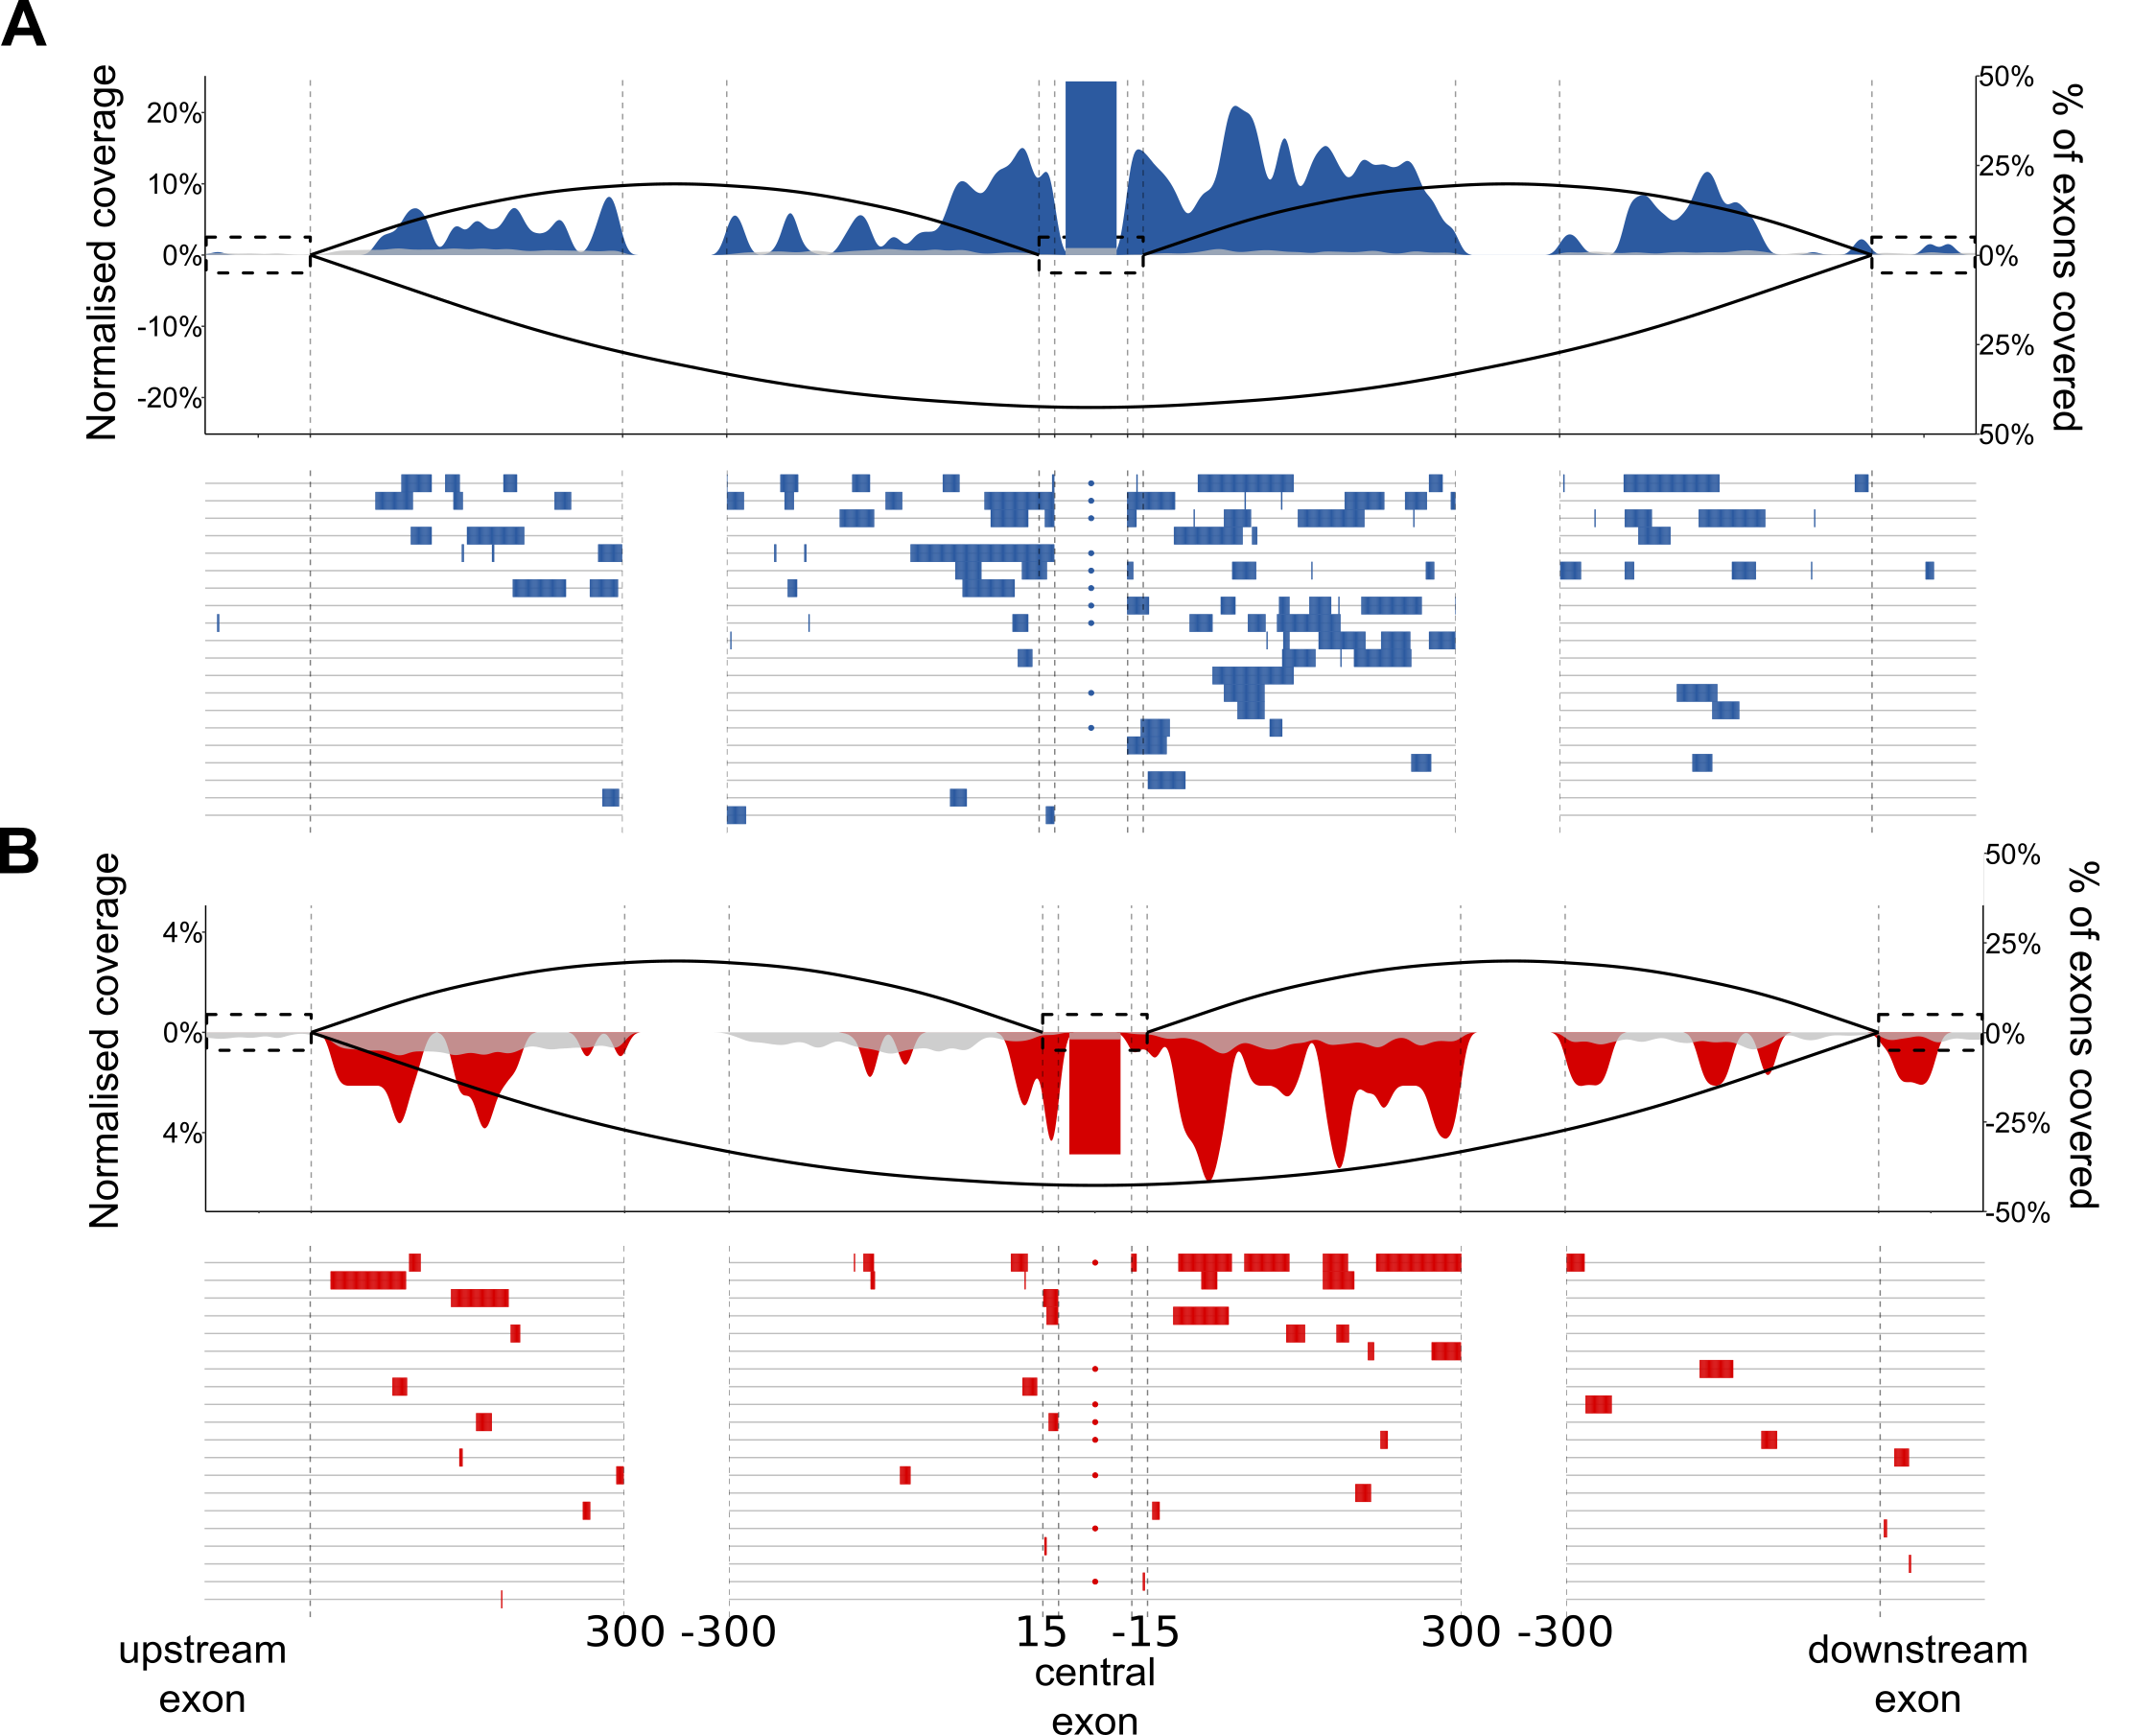
\includegraphics[width=\textwidth]{Figures/05_tdp_mice/iclip_multipanel.png}
	\caption[RNA maps of skiptic and cryptic exons show direct binding by TDP-43]{
		\textbf{RNA maps of skiptic and cryptic exons show direct binding by TDP-43.}
	\textbf{(A)} The 33 cryptic exons found in the RRM2mut embryonic mice. Traces show normalised iCLIP peak coverage within and around each exon. Left y-axis: the proportion of exons with an iCLIP peak at that nucleotide. Right y axis: the proportion of central exons or flanking exons that overlap any iCLIP peaks. Below, individual positions of iCLIP peaks for the top 20 cryptic exons. Circles in the centre denote whether there are any iCLIP peaks overlapping the central exon. 
	\textbf{(B)} as before for the 48 skiptic exons found in the LCDmut adult mice.
}
	\label{iclip_multi}
\end{figure}

Cryptic exons associated with TDP-43 depletion have been demonstrated to originate from mRNA that is directly bound by TDP-43 itself \citep{Ling2015}. 
This suggests that these splicing changes emerge because TDP-43 can no longer act to repress cryptic exon recognition by the splicing machinery and other factors. 
I remade the RNA maps for iCLIP protein-RNA interaction peaks for the 33 cryptic and 48 skiptic exons found in RRM2mut and LCDmut to test whether they appeared to be directly bound by TDP-43. 
The RRM2mut cryptic exons show overlapping and closely flanking TDP-43 binding and strikingly so do the LCDmut cryptic exons. 
Importantly, the iCLIP data used for these maps is mainly drawn from wildtype TDP-43, suggesting that while TDP-43 may be normally binding the skiptic exons it does not do so sufficiently strongly to repress their inclusion. 

\begin{table}
	\begin{footnotesize}
	\begin{tabular}{llll}
		& total & overlap	& \% \\
		\hline
		All exons in GENCODE vM12 &	744,786	& 37,276 & 5\% \\
		All constitutive exons found in all samples	& 239,897	& 17,828	& 7.4\% \\
		All cassette exons found in all samples &	5,656 &	361	& 6.4\% \\
		Significant cassette exons (FDR < 0.05) between LCDmut and wildtype mice	& 260	& 49 & 18.8\% \\
		Skiptic exons (control PSI > = 0.95; dPSI > = -0.05; FDR < 0.05) & 47 &	31 & 66\% \\
	\end{tabular}
	\end{footnotesize}
	\caption[Proportions of exons with any TDP-43 binding from iCLIP]{\textbf{Proportions of exons with any TDP-43 binding from iCLIP}}
	\label{tab:iclip_proportions}
\end{table}


\subsection{Skiptic splicing is predicted to be deleterious to gene expression}

\begin{figure}[h!]
	\centering
	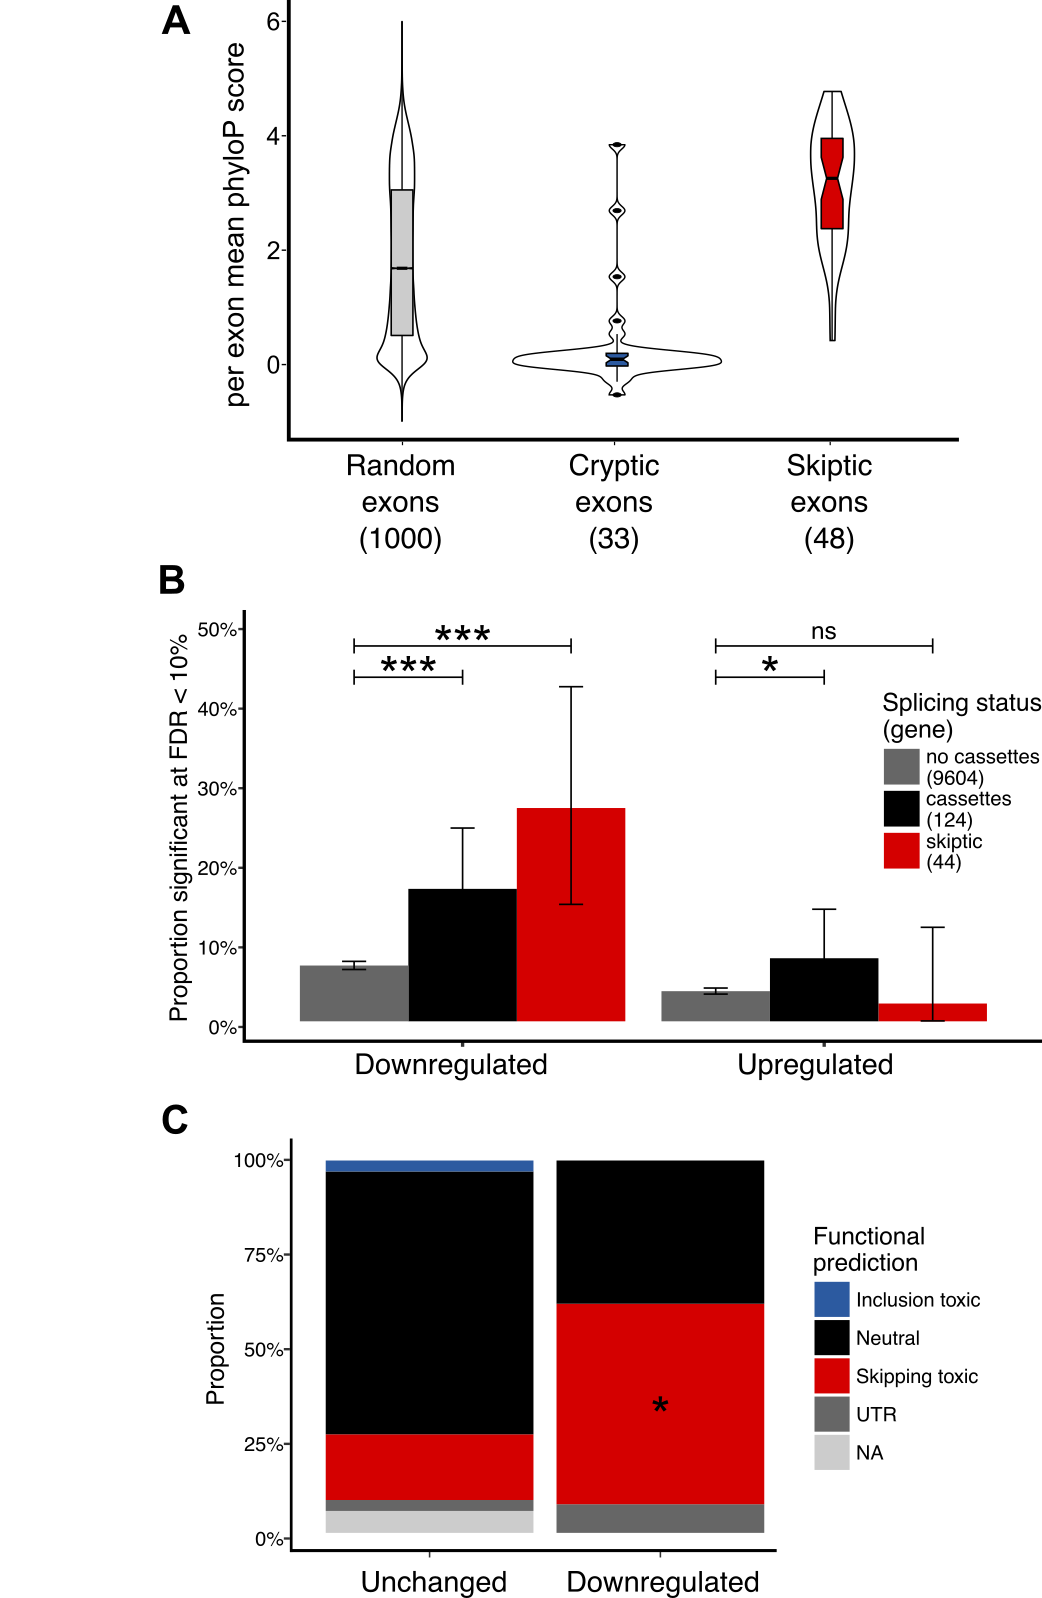
\includegraphics[width=9cm]{Figures/05_tdp_mice/functional_plots_vertical.png}
	\caption[Functional analyses of the skiptic exons]{
		\textbf{Functional analyses of the skiptic exons.}
	\textbf{(A)} Per-exon mean PhyloP conservation scores presented as box plots for each set of exon, showing the median and interquartile range. Notches are the 95\% confidence interval of the median. 
	\textbf{(B)} The relationship between splicing status and differential expression in LCDmut. Significantly downregulated genes (FDR < 0.1) are enriched in skiptic exons compared to genes expressed at a similar level (\textit{P}=1.19e-6), as well as non-skiptic cassette exons (\textit{P}=6.16e-5). Upregulated genes are mildly enriched in non-skiptic cassette exons (\textbf{P}=0.029) but not in skiptic exons (\textbf{P}=0.88). All \textit{P}-values generated from a binomial test. 
	\textbf{(C)} Proportions of predicted downstream consequence of exon skipping for either non-regulated or downregulated skiptic exons. \textit{P}=0.034; chi-squared test.
}
	\label{fig:functional_plots}
\end{figure}

Cryptic exons originate from very poorly conserved DNA sequence  (Fig. \ref{fig:functional_plots}A), suggesting that there is no functional protein coding information encoded in them. 
Inclusion of these essentially randomised sequences would more likely than not lead to degradation of the host mRNA transcript through the inclusion of premature stop codons or frameshifts and nonsense-mediated decay.
Skiptic exons are highly conserved (Fig. \ref{fig:functional_plots}A), with a much higher average conservation level than a randomly chosen set of annotated exons from GENCODE.  
This is to be expected from their close to 100\% inclusion rates within transcripts. 
Their constitutive splicing status means that their inclusion is near guaranteed and so unlike cassette exons, which are swapped in and out dynamically between tissues and developmental time points, I hypothesis that there is no evolutionary pressure to maintain a length divisible by 3. 
In the event of these exons being skipped they would likely lead to a shift of reading frame, potentially leading to degradation of the host transcript through nonsense-mediated decay.
 To test whether skiptic exon splicing correlated with host transcript degradation I combined the differential splicing and differential expression analyses together. I separated genes into sets based on i) whether they were significantly upregulated or downregulated in LCDmut compared to wildtype (FDR < 10\%) and ii) whether they contained either a cassette exon or a skiptic exon that changed in inclusion levels between LCDmut and wildtype (FDR < 1\%). 
 Genes that contained skiptic exons were more likely to be downregulated than those without any cassette exon splicing  (\textit{P}=1.19e-6; binomial test; Fig. \ref{fig:functional_plots}B). The same trend cannot be seen in the other direction as there as no increased likelihood for skiptic containing genes to be upregulated. 
 Finally I attempted to predict \textit{in silico} whether the skipping of a skiptic exon would lead to nonsense mediated decay. 
 By combinining the central cassette exon with the flanking upstream exons and translating the concatenated sequence it is possible to assess whether skipping the central exon would frameshift the downstream exon, generating premature stop codons. 
 Using this method I discovered that 15 out of 47 of the skiptic exons would lead to the inclusion of a premature stop codon.  
I compared the distribution of predictions between skiptic exons in downregulated and unchanged genes and found an increased representation of predictions of toxic skipping from 18\% to 54\% (\textit{P}=0.034; chi-squared test). 

\subsection{LCDmut impairs TDP-43 autoregulation}

\begin{figure}[h!]
	\centering
	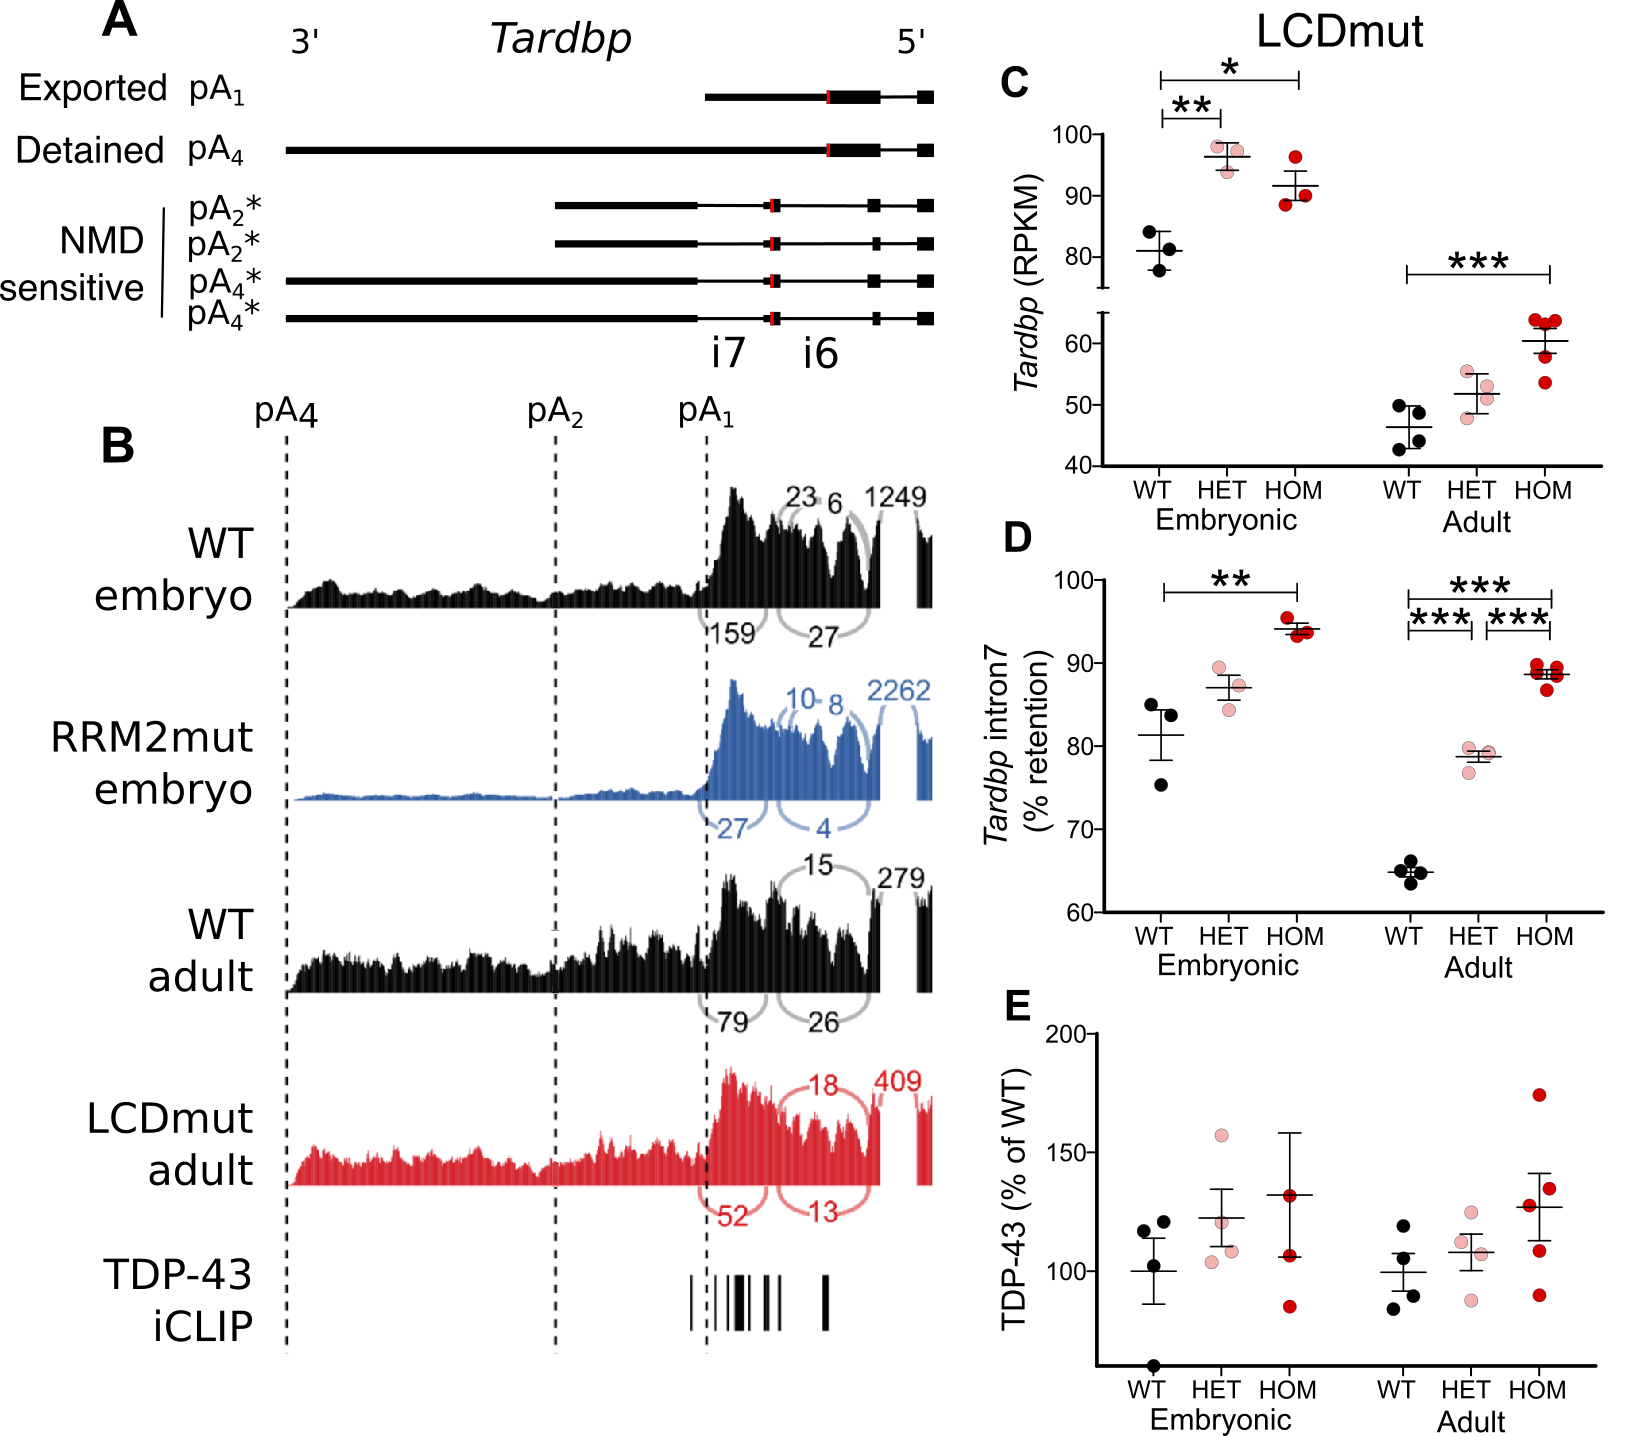
\includegraphics[width=\textwidth]{Figures/05_tdp_mice/autoregulation.png}
	\caption[LCDmut and TDP-43 autoregulation]{
		\textbf{LCDmut and TDP-43 autoregulation.}
	\textbf{(A)} The 3'UTR of \textit{Tardbp}. At least six potential 3'UTR isoforms have been proposed by \citep{Koyama2016}, consisting of 3 different polyadenylation (pA) sites. * indicates that this isoform is predicted to be degraded by nonsense-mediated decay. Stop codons indicated by red bars. 
	\textbf{(B)} Expression of all \textit{Tardbp} isoforms (RPKM) increases in LCDmut at two time points.  Embryonic dataset ANOVA, \textit{P}=0.0032, \textit{n}=3; adult dataset ANOVA, \textit{P}=0.0009, \textit{n}=4$-$5; error bars: SD; Bonferroni multiple comparison tests are plotted as \textit{P}-value: *\textit{P} < 0.05; **\textit{P} < 0.01; ***\textit{P} < 0.001
	\textbf{(C)} Retention of 3'UTR intron 7 increases in LCDmut. Embryonic dataset ANOVA, \textit{P}=0.0113, \textit{n}=3; adult dataset ANOVA, \textit{P} < 0.0001, \textit{n} = 4$-$5; error bars: SEM; Bonferroni multiple comparison tests are plotted as \textit{P}-value: **\textit{P} < 0.01; ***\textit{P} < 0.001.
	\textbf{(D)} Quantification of TDP-43 protein levels in relation to $\beta$-actin in Western blots. Results are normalised to the mean of wildtype (100\%). Embryonic dataset: ANOVA \textit{P}=0.480, \textit{n}=4; adult dataset: ANOVA \textit{P}=0.491, \textit{n}=3; error bars: SD.
}
	\label{fig:autoregulation}
\end{figure}

Many RNA-binding proteins have been shown to regulate their own translation, this is termed autoregulation \citep{Lareau2007,Wollerton2004}]. 
When levels of the protein are high they will bind to their mRNA and shift production to an untranslated isoform, through nonsense-mediated decay or through nuclear retention \citep{McGlincy2008-wh,Boutz2015}.
The 3' untranslated region (3'UTR) of \textit{Tardbp} is remarkably complex regulatory hub (Fig. \ref{fig:autoregulation}A). 
There are 3 experimentally validated polyadenylation and cleavage sites, pA1, 2, and 4. 
There also 2 introns within the 3'UTR (6 and 7; \citep{Ayala2011,Koyama2016}). 
3'UTR splicing is a mechanism for regulating TDP-43 translation as an intron that follows a stop codon should trigger nonsense-mediated decay. 
Both spliced isoforms pA$_2$* and pA$_4$* are predicted to undergo nonsense-mediated decay due to the stop codon is further than 50bp from the intron in each.
Additionally, the long pA4 site is preferentially retained in the nucleus where it is degraded by the exosomal complex \citep{Ayala2011}.
Only the pA1 isoform is translated into TARDBP protein \citep{Koyama2016}.
TDP-43 binds the 3'UTR of its own mRNA overlapping the pA$_1$ site  \citep{Polymenidou2011,Tollervey2011}.
This prevents polyadenylation at the pA1 site and encourages the creation of the retained pA4 transcript and the splicing of NMD-sensitive pA$_2$* and pA$_4$* isoforms \citep{Koyama2016}. 
This system allows TDP-43 protein levels to regulate the stabilty of \textit{Tardbp} mRNA.

I assessed the the \textit{Tardbp} 3'UTR locus in the RNA-seq data to observe whether the two mutations had effects on autoregulation. 
RRM2mut shifts the balance of UTR isoforms from near equal amounts of pA$_1$ and pA$_4$ to predominantly pA$_1$, presumably due to its reduced RNA binding ability  (Fig. \ref{fig:autoregulation}A).  
In LCDmut, a clear upregulation of Tardbp mRNA expression is seen in both embryonic and adult RNA-seq samples (Fig. \ref{fig:autoregulation}B). 
When I quantified the level of intron 7 inclusion,  a proxy for the proportion of NMD-sensitive pA$_2$* and pA$_4$* isoforms, LCDmut increased intron 7 retention in a dose dependent manner, suggesting a loss of NMD-sensitive UTR isoforms (Fig. \ref{fig:autoregulation}C). 
However, when assessing the total TDP-43 protein levels by Western blotting, no difference was observed between LCDmut and wildtype cells (Fig. \ref{fig:autoregulation}D).
Together this suggests a subtle impairment in the autoregulation feedback loop in LCDmut cells.

\subsection{Skiptic splicing can be observed in human ALS patients}
% work performed by Pras - show RT-PCRs
% explain dodgy quantification
\begin{figure}[h!]
	\centering
	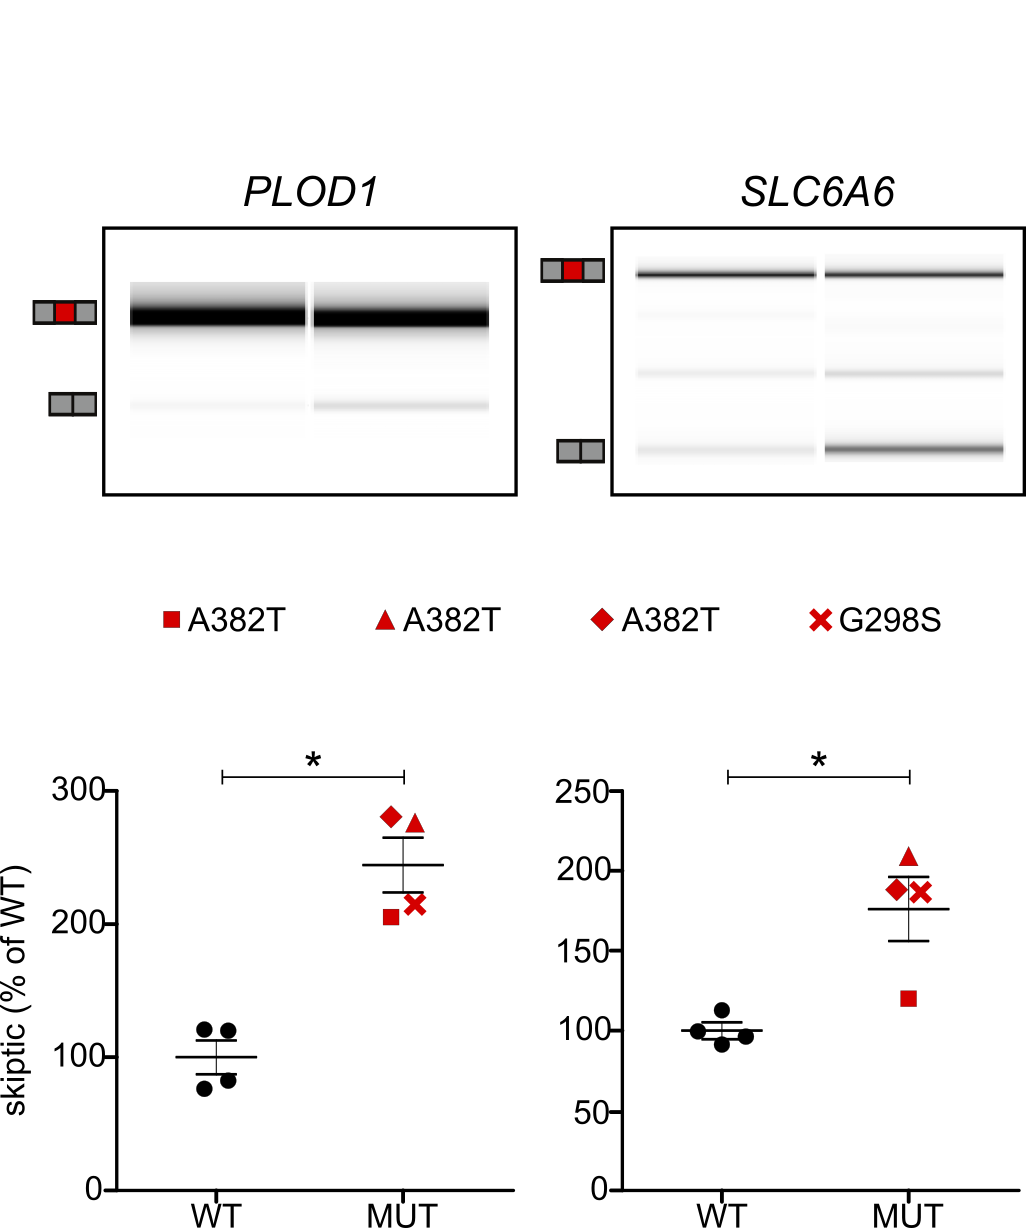
\includegraphics[width=10cm]{Figures/05_tdp_mice/skiptic_patients.png}
	\caption[Skiptic exon splicing in TARDBP ALS]{
		\textbf{Skiptic exon splicing in TARDBP ALS.}
		RT-PCR traces for two skiptic exons in fibroblasts taken from 4 \textit{TARDBP} ALS patients and 4 non-neurological control lines. For clarity, quantification was taken of the skiptic exon band only instead of the ratio. *\textit{P} < 0.05, \textit{n} = 4, error bars: SEM
	}
	\label{fig:skiptic_patients}
\end{figure}

Due to the high species conservation of the skiptic exons, I reasoned that it might be possible to see evidence of their skipping in human ALS patients with heterozygous mutations in the low complexity region of \textit{TARDBP}. Seven skiptic exons were tested using RT-PCR in four patients with the A382T and G298S mutations and four control fibroblast lines. 
Two skiptic exons were found to have a mild but statistically signficant increase in the intensity of the band matching the skipping transcript.	
This provides the first evidence of a gain of TDP-43 splicing function in patients with ALS-associated \textit{TARDBP} mutations.

\clearpage

\section{Discussion}

In this study  two complementary mouse models were developed to study the splicing function of TDP-43. 
%Benefits of knock-in mutations
%RRM2mut is softer LOF - allows mice to live longer and us to study embryonic tissues - role in development? Cite Modic paper
By using point mutations I have been able to observe the modulation of TDP-43-regulated splicing without dramatically altering TDP-43 expression. 
This has been particularly useful when studying RRM2mut. 
TDP-43 is very highly expressed during embryonic development and knockout mice die at E6.5 \citep{Ricketts2014}) whereas RRM2mut mice survive until E18.5, allowing greater scope for studying TDP-43 loss in development.
We have conclusively proven RRM2mut to be a loss-of-function mutation through our experiments on known TDP-43 splicing targets and also by looking transcriptome-wide. 
This is also shown by the observation of widespread cryptic exon inclusion and the downregulation of long intron genes, two clear molecular phenotypes of TDP-43 loss.

LCDmut is an intriguing mutation as I have discovered a completely novel and unexpected gain of splicing function. 
RNA maps demonstrated that the splicing targets altered in LCDmut are enriched in TDP-43 binding through iCLIP data, even when using iCLIP from wildtype TDP-43. 
This suggests a shift from TDP-43 binding from passive to active regulation at these loci.

Although in the fibroblast data there are a small number of overlapping exons that are spliced in opposing directions, the majority of exons altered in LCDmut are not changed in RRM2mut. 
This suggests that regulation of these exons is not simply bi-directional, with LCDmut increasing TDP-43 to cause skipping of an exon at sites where its loss causes inclusion.

One hypothetical mechanism for the gain of splicing function seen in LCDmut is through an impairment of TDP-43 autoregulation which would increase TDP-43 protein levels.
The splicing of intron 7 decreases in a dose-dependent manner with LCDmut, suggesting a reduction in the creation of NMD-sensitive 3'UTR isoforms.
It is curious that this is reflected with a clear increase of \textit{Tardbp} mRNA but not at the protein level.
This may be due reduced sensitivity of western blotting when compared to RNA-seq, or that the Western blotting was carried out on total cellular protein rather than fractionated by cellular compartment.
Mice that are heterozygous for a TDP-43 null allele show altered autoregulation without changes in TDP-43 protein levels either \citep{Ricketts2014} so they may well be a more subtle effect on translation than it is currently possible to detect. 

The most unexpected finding in LCDmut is the discovery of skipped constitutive exons: skiptic exons. 
Previously TDP-43 had only been studied in the context of alternate cassette exons.
Whereas cryptic exons emerge from normally repressed sections of introns that contain strong splice sites, skiptic exons appear to be an over-correction by TDP-43.
Focusing our RNA maps on these skiptic exons shows that both cryptic and skiptic exons are similarly enriched by TDP-43 binding in wildtype cells.
Therefore TDP-43 may have a minor role in supporting the inclusion of these exons but with the LCDmut mutation this shifts to promoting their excision from the host transcript.
That I see only 44 genes affected by skiptic transcripts may be down to the sheer redundancy and collaboration between multiple RNA-binding proteins. 
The skiptic exons may represent transcripts that are most sensitive to TDP-43 expression for their correct splicing, but why they do not also show changes in TDP-43 loss is mysterious.

Cryptic exons show a higher enrichment for TDP-43 iCLIP peaks than the skiptic exons. 
This is potentially an artefact of comparing iCLIP from predominantly embryonic tissue with splicing changes from adult mice but it could point to an alternate mechanism to explain the gain of splicing function.
Low-complexity domains are crucial for assembling RNA-binding proteins into structures  \cite{Gueroussov2017} and its possible that the LCDmut mutation shifts TDP-43 into assembling more strongly with certain groups of proteins to play a stronger role in splicing regulation at certain loci. 
Experiments to determine the protein-protein "interactome" of TDP-43 have been published \citep{Freibaum2010-hw} and it would be intriguing to compare LCDmut to wildtype TDP-43. 

Recently a study investigated a similar model of TDP-43 ALS where the ALS patient mutation Q331K was knocked in to mice \citep{White2018}. 
They reported a similar gain of splicing function in the homozygous mice, although they looked at a small number of individual splicing events and not transcriptome-wide.
They also observed an increase in \textit{Tardbp} mRNA levels which was accompanied by an increase in \textit{nuclear but not cytoplasmic} TDP-43 protein levels.
The assay (Fig. \ref{fig:autoregulation}D) looked at total TDP-43 protein levels so this may explain why no difference was seen. 
Together the two studies convincingly show that mutating the low-complexity domain of TDP-43 leads to changes in autoregulation and gain in splicing function.
It would be interesting to see whether the skiptic exons observed in adult LCDmut spinal cord can be detected in the now published Q331K frontal cortex.
Another recent study used a BAC transgenic mouse of either wildtype human TDP-43 or ALS patient mutation M337V \citep{Gordon2018}.
 
 My work on the long intron genes and the RNA maps raises interesting questions about the role of TDP-43 in splicing beyond merely binding on top of or closely flanking splice sites. 
 The cassette exons altered in either RRM2mut or LCDmut show enrichment in TDP-43 iCLIP peaks in the distal introns, albeit at a lower intensity. 
 The long-intron genes that are downregulated selectively in RRM2mut also show a general enrichment in iCLIP peaks throughout the intron.
 Conversely, the upregulated long genes are depleted in iCLIP peaks compared to other upregulated genes.
 Together this suggests perhaps an additive role in splicing, where the introns that can be bound by as many molecules of TDP-43 will be processed differently, overriding the need for targeted TDP-43 binding to splice sites.
 This will be interesting to explore with future datasets, with iCLIP at greater sequencing depth. 

 
 % skiptic validation woes
 The two skiptic exons validated in human ALS patients are intriguing high quality transcriptome-wide data is needed to determine whether TDP-43 gain of splicing function is occurring in patient cells.
 Although the skiptic exons should be conserved between mouse and human, the flanking regulatory sequences that flank the exons may not, so it is not surprising that only two of the seven skiptic exon candidates could be seen to change. It has been previously reported that TDP-43 depletion has a different effect size on the same exon in human than in mouse \cite{Mohagheghi2016}. 
 This is supposedly due not to TDP-43 binding, which is invariant, but the role of other RNA-binding proteins.
This combinatorial model of splicing is currently intractable to investigate transcriptome-wide. % reference in discussion
 
 % skiptics, cryptics and sporadic ALS
 While our human validation work was on patients with \textit{TARDBP} mutations, it is interesting to speculate on the relevance of TDP-43 splicing to sporadic disease. 
 Increased total and cytoplasmic \textit{TARDBP} mRNA has been observed in sporadic ALS patient neurons, particularly in neurons with TDP-43 aggregations \citep{Koyama2016}.
 One can imagine a scenario whether altered TDP-43 autoregulation in sporadic ALS would initially over-compensate and increase \textit{TARDBP} mRNA and cause a splicing gain of function.
 Eventually when TDP-43 is completely unable to enter the nucleus there would be a shift to a TDP-43 loss of function phenotype, heralded by cryptic exon inclusion and long intron gene downregulation.  
 This idea would be interesting to test in a longitudinal human cell model, for example ALS patient stem cell-derived motor neurons.
 
 LCDmut mice exhibit symptoms of motor neuron degeneration (decreased motor neuron numbers, reduction in grip strength - data not shown), but do so without TDP-43 aggregation in motor neurons. 
 This uncoupling of TDP-43 aggregation and disease symptoms has been observed in other TDP-43 mutant mouse models \citep{Arnold2013, Gordon2018}.
 
 % mechanistic work - repeating myself
 Further work is needed to untangle the mechanism by which a low-complexity domain mutation leads to a gain of splicing function.
 As well as pursuing the change in autoregulation and what this might do to TDP-43 translation, I believe it is worth investigating changes in the TDP-43 interactome such a mutation might cause.
 
 
 %UGUG is the strongest motif bound by TDP-43 but it is not the only one. 
 %With a more nuanced approach
%RRM2mut - fully expected to see cryptic exons and long genes
%
%LCDmut is novel - GOF
%
%some overlap - seen in MEFs, but mostly unique targets - suggesting distinctive mechanisms
%
%ideas for mechanism
%	impaired autoregulation
%	We found changes in intron 7 splicing and increased overall Tardbp expression but no changes at the protein level
%	Westerns too subtle? Or the protein increase is localised to the nucleus
%	change in UTR splicing but no change in protein levels - seen before by Ricketts and ...
%	altered proteome  - Mogheghi paper, Freibaum etc
%	
%LCDmut lacks TDP-43 mislocalisation, cryptic exons and long gene downregulation
%
%Jemeen paper - Q331K also has a gain of splicing function and changes in autoregulation
%	They did not look transcriptome wide
%	Interesting to observe any evidence of skiptic exons
%
%Long range effects on splicing 
%	RNAmaps show enrichment in distal splice sites of iCLIP and motifs
%	TDP-regulated introns 
%	Long genes have increased coverage throughout whole intron - some kind of additive effect?
%	
%Further work
%	GOF and LOF in disease progression
%	Validate the skiptics in more patients and human models of ALS progression
%	Be smarter about picking skiptics to validate - cite that paper comparing human and mouse SORT1 inclusion - more than just UG
%	
%	How applicable is a patient-like mutation to sporadic ALS? Increased cytoplasmic TDP mRNA has been seen in patient cells (Koyama 2016)


%	Caveats - probably put in main discussion chapter as they apply to all work
%		Full extent of TDP-43 regulated splicing is still unclear - sample sizes still too small
%		SGSeq methods give us all cassettes without being biased by annotation
%		Still can't resolve complex splicing changes
%		iCLIP is not combinatorial - only explores a single RBP and says nothing about co-operation or redundancy.  Julian Koenig has some in vitro iCLIP that looks at this
%		Most of the data is still ignored - TDP-43 affects 3'UTR splicing (Gregor paper) and we neglect this, DNA binding and chromatin remodelling which are all affected simultaneously.

% % probably for general discussion
%Existing RNA-protein interaction experiments examine the binding of a single protein. What is currently lacking are techniques for exploring combinatorial interactions between many different RNA-binding proteins. The cryptic and skiptic exons found in this study are most likely representing the sections of transcriptome most vulnerable to the depletion or overexpression of a single protein, TDP-43.

		
\section{Summary}



\chapter{ALS-causative FUS mutations impair FUS autoregulation through intron retention}

\label{chapter:fus_meta}

\section{Overview}

The most aggressive FUS mutations in ALS are those that completely abolish the nuclear localisation signal (NLS). 
Patients carrying a single copy of the P525L mutation, where the critical proline of the PY motif is mutated \citep{Chio2009}, die around 20 years of age with a disease course of less than 2 years \citep{Shang2016}.
The removal of the NLS mislocalises FUS to the cytoplasm but whether toxicity comes from reducing the nuclear functions of FUS or through a new function in the cytoplasm is still being debated.

The Fratta lab generated RNA sequencing data from embryonic mouse neuronal tissue where FUS was either knocked out or the NLS removed through mutation. I combined the data with two previously published datasets with similar NLS mutations and FUS knockout mice. 
To assess differential expression and splicing I employed a joint modelling strategy which boosted the power of detection and increased the confidence in my findings. 
I found that in both expression and splicing, FUS NLS mutations act as a diminished knockout, with little evidence to support a gain of toxic function in the cytoplasm. 
When examining FUS itself, I observed that loss of nuclear FUS correlated with the reduction in the splicing of a retained intron transcript, which was validated by RT-PCR. 
The FUS intron retention transcript is insensitive to nonsense-mediated decay.
My data suggest that disease-associated FUS mutations impair FUS autoregulation which is normally maintained through a retained intron transcript. This work has important implications for both the RNA biology and neurodegenerative disease fields.



\section{Contributions}
\begin{itemize}
	% Check with Pietro
	\item Mice were handled by Dr Cristian Bodo
	\item RNA sequencing libraries were prepared by Dr Nicol Birsa.
	\item RNA was extracted for PCR by Dr Nicol Birsa and Matthew Bentham
	\item Primers designed and RT-PCRs were performed by David Robaldo and Dr Carmelo Milioto
	\item Methods for RT-PCR were written by David Robaldo
\end{itemize}
All bioinformatic analysis and interpretation was designed and performed by myself.  
The validation experiments were designed by myself and Dr Pietro Fratta.

\clearpage
\section{Background}


\begin{figure}[h!]
	\centering
	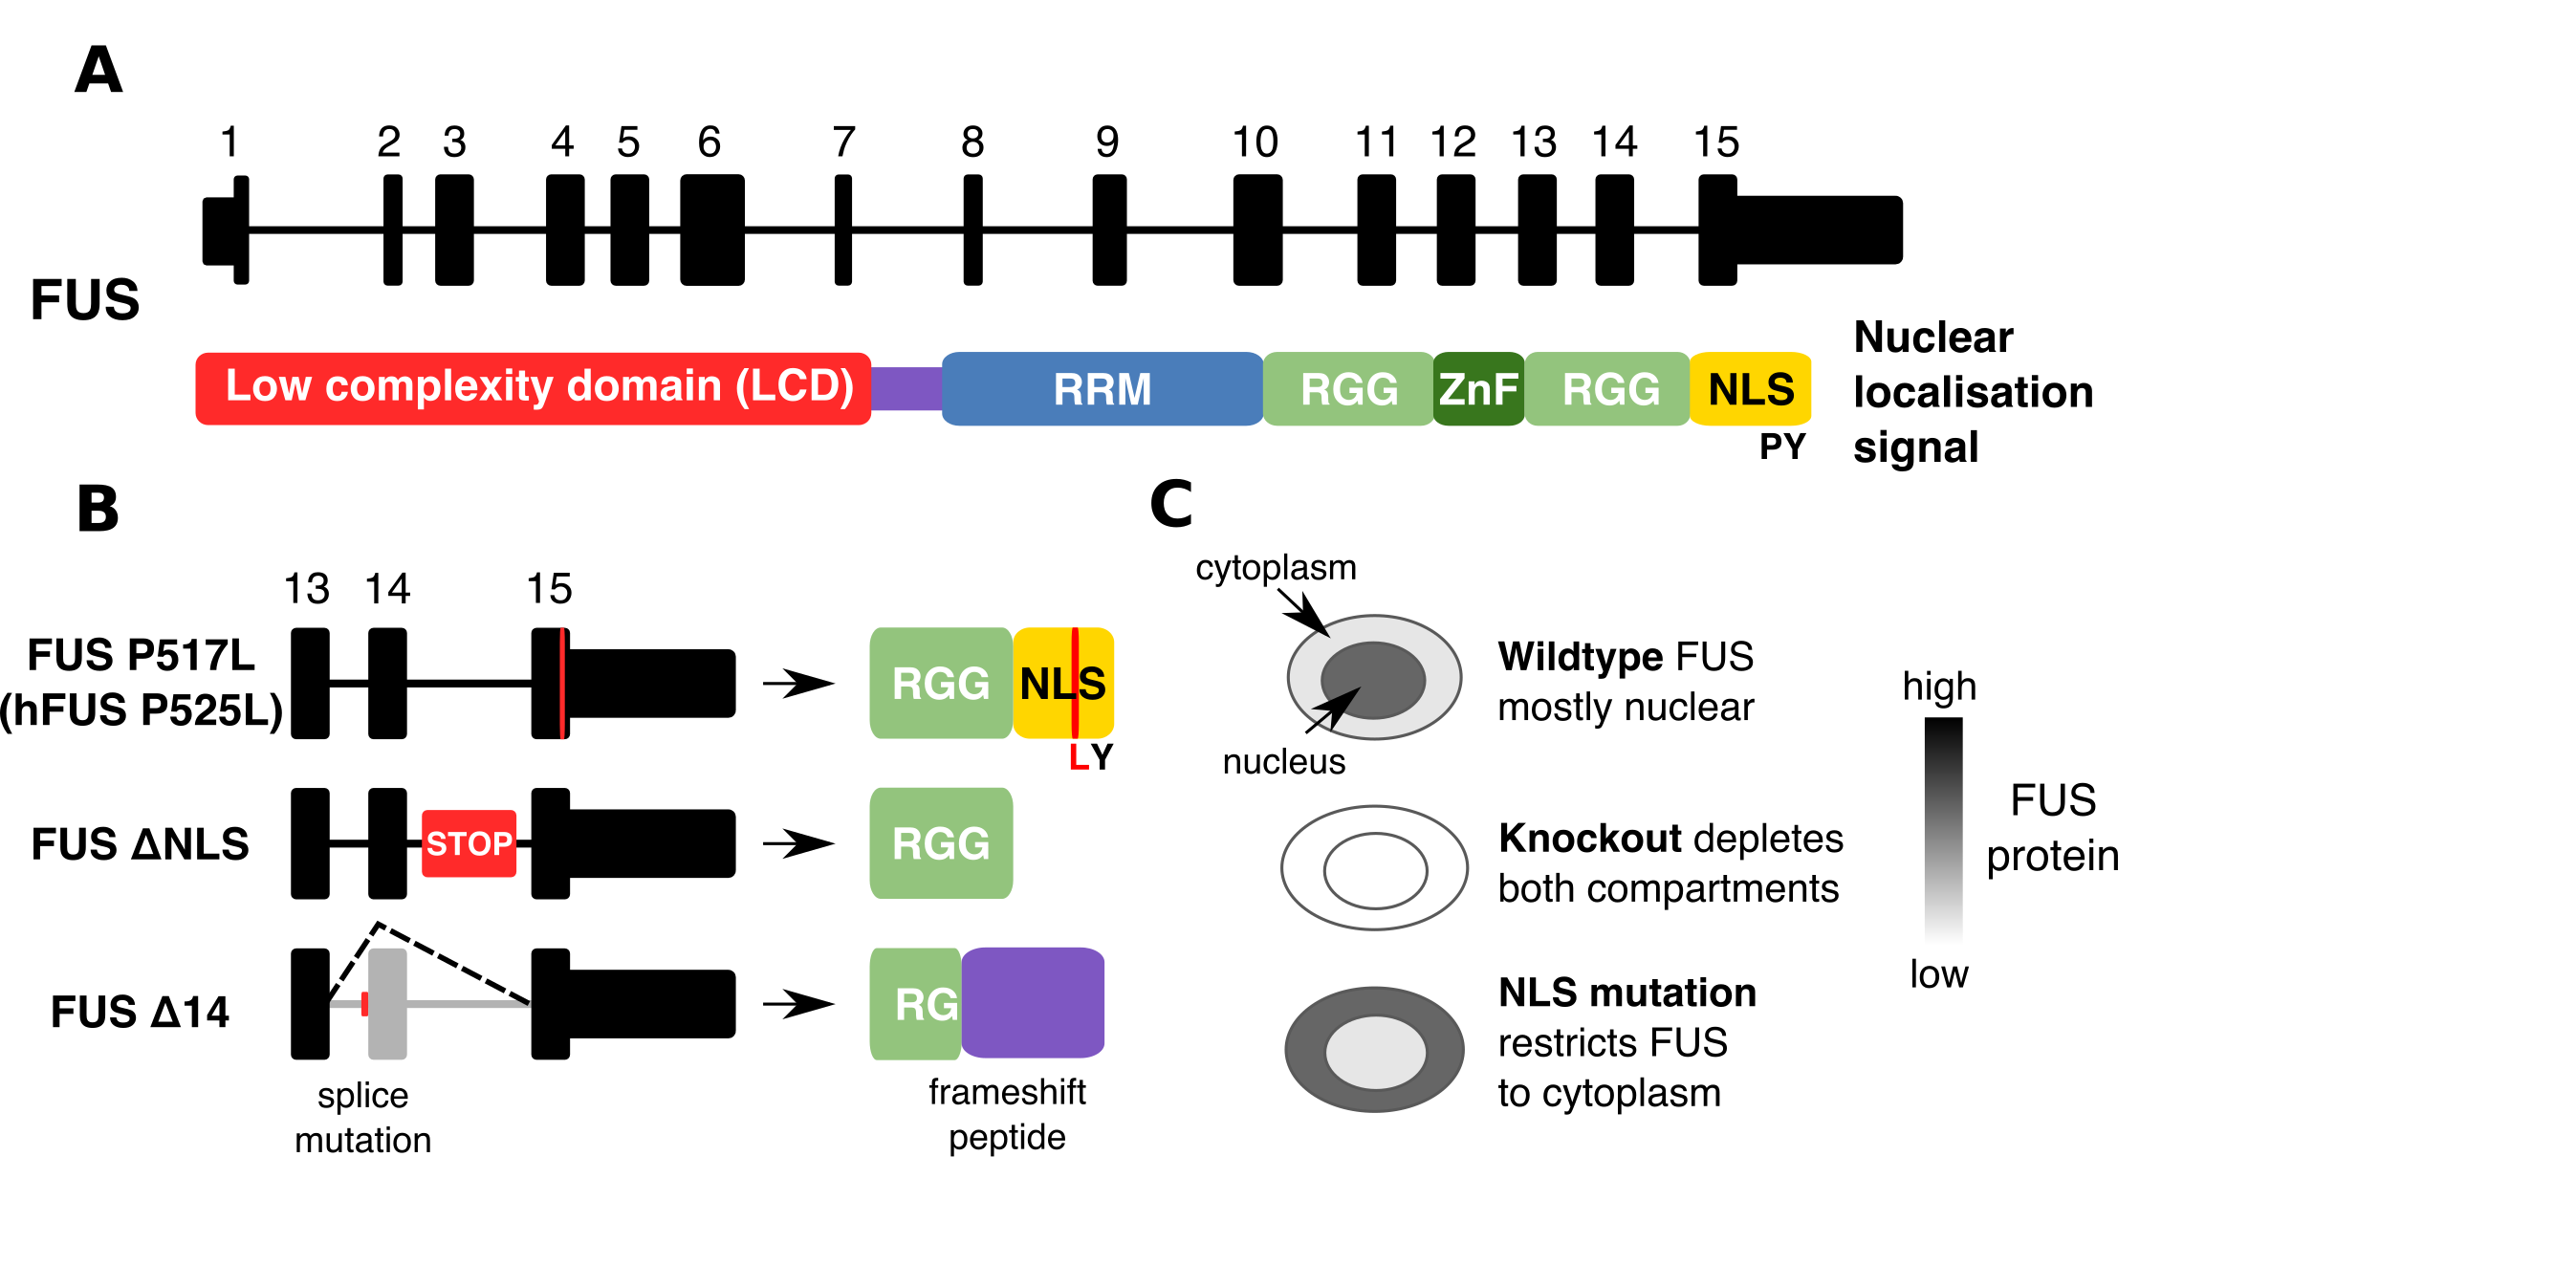
\includegraphics[width=\textwidth]{Figures/06_fus_meta/FUS_structure_mutations.png}
	\caption[The structure of the FUS protein and known ALS mutations]{
		\textbf{The structure of the FUS protein and known ALS mutations}.
		\textbf{(A)} The FUS protein is comprised of a low complexity domain (LCD), an RNA recognition motif (RRM) domain, two Arginine-Glycine-Glycine (RGG) domains, a zinc finger domain (Znf), a nuclear export signal (NES) and a nuclear localisation signal (NLS). 
		\textbf{(B)} The three FUS NLS mutations used in this study. The Bozzoni group knocked in a point mutation to create the FUS P525L line, a missense mutation equivalent to the human ALS P517L mutation.  
	The Dupuis group created a FUS $\Delta$NLS line where the entire NLS is removed.  
	We have used the FUS $\Delta$14 mouse, where a frameshift mutation leads to the skipping of exon 14 and a frameshifting of the remaining NLS sequence.
	\textbf{(C)} In wildtype  cells FUS protein is predominantly nuclear but can shuttle to the cytoplasm. When FUS is knocked out it will be reduced in both compartments but if the NLS is mutated or deleted then FUS will accumulate in the cytoplasm.
}
	\label{fig:fus_structure}
\end{figure}


% Discuss 3 datasets, pros and cons of each
% differences in sequencing, prediction
For this study, three datasets of FUS knockout and FUS nuclear localisation signal mutation were used. When combined I refer to them collectively as FUS KO and FUS MUT respectively. Table \ref{tab:fus_datasets} describes the 3 datasets. Table \ref{tab:fus_sequencing} describes the sequencing libraries generated.

\subsubsection{Bozzoni}
Capauto and colleagues from the Bozzoni group generated RNA-seq data from purified motor neurons cultured from mouse induced pluripotent stem cells \citep{Capauto2018}. 
Their knockout uses a gene trap in \textit{Fus} intron 12 first used by Hicks et al \citeyear{Hicks2000}.
This construct leads to a partial reduction of FUS protein levels.
Their NLS mutation is the P525L point mutation \citep{Chio2009}, which in mice corresponds to P517L.  
All mice are homozygous for their transgenes. 
The two conditions share a single set of controls, which are motoneurons derived from wildtype stem cells.
The read depth and length for all the Bozzoni samples is high  and but the sample number is n=3 for each condition, the lowest of the three datasets.
%The sequencing libraries are total RNA rather than polyA enriched which may impact the between-sample variance and make splicing events harder to interpret.
Their differential expression analysis found 40 genes in common, with 198 specific to knockout and 419 specific to NLS mutation. 
Splicing changes were not assessed in their publication.

%Dupuis
\subsubsection{Dupuis}
Scekic-Zahirovic and colleages from the Dupuis group generated RNA-seq data from mouse embryonic brain (embryonic day E18.5) \citep{Scekic-zahirovic2016}. 
Their knockout construct uses a gene trap in \textit{Fus} intron 1 (generated in-house) which leads to complete FUS loss.  
Their NLS mutation introduces a stop codon after exon 14, terminating transcription upstream of the NLS sequence ($\Delta$NLS).  
This mimics the R495X mutation which removes the entire NLS sequence \citep{Bosco2010}.
All mice are homozygous for their transgenes. 
The two conditions have their own separate wildtype littermate controls. 
The depth and read length of the RNA-seq libraries is lower than the other two datasets but this is compensated for by being polyA+ enriched, which will mean a greater proportion of sequencing reads aligning to coding exons.  
%This will be useful for assessing differential expression but I predict the dataset will not be particularly useful for differential splicing due to the low read depth and read length.
They found a strong overlap between differentially expressed genes in the two transgenic lines, with 353 shared genes, 433 specific to FUS NLS mutations and 1205 specific to FUS knockout. 
They also performed a targeted cassette exon splicing analysis (RASL-seq) and again found overlap between knockout and NLS mutation, with 75 shared cassette exons, 98 specific to NLS mutation and 177 specific to knockout. 

% Fratta
\subsubsection{Fratta}
The third dataset was created for this study by the Fratta group from mouse embryonic spinal cord samples (embryonic day E18.5).
 The knockout construct used to generate mice is the same as the Dupuis dataset and hence should be a robust knockout of FUS. 
The NLS mutation is the $\Delta$14 mutation discussed in the previous chapter. A splice acceptor site mutation in exon 14 site prevents exon inclusion, leading to a downstream frameshift and removal of the NLS. 
This mutation corresponds to the human G466VfsX14 mutation \citep{DeJesus-Hernandez2010}.
Each condition, $\Delta$14 and knockout have their own wildtype littermate samples as controls. 
For both conditions, heterozygous mice with only one mutant allele were also generated and sequenced.
The RNA-seq data produced has the longest reads at 2 x 150bp as well as high sequencing depth.
This provides sufficient resolution to quantify differential splicing.\newline

By combining the newly generated Fratta dataset with that of the two previous groups I have put together the largest analysis to date on FUS and gene expression. 
Furthermore I have performed a comprehensive analysis on splicing, looking for both annotated and novel splicing events in both FUS knockout and NLS mutation.
This joint modelling approach boosts statistical power and allows me to demonstrate that the majority of differentially expressed genes and differential splicing events are shared between FUS knockout and NLS mutation.

\clearpage






\section{Methods}

\subsection{RNA sequencing}


\begin{longtable}[t]{@{}llllll@{}}
	\begin{minipage}[t]{0.14\columnwidth}\raggedright\strut
		{\textbf{Dataset}}\strut
	\end{minipage} & \begin{minipage}[t]{0.14\columnwidth}\raggedright\strut
		{\textbf{Tissue}}\strut
	\end{minipage} & \begin{minipage}[t]{0.12\columnwidth}\raggedright\strut
		{\textbf{Controls}}\strut
	\end{minipage} & \begin{minipage}[t]{0.10\columnwidth}\raggedright\strut
		{\textbf{Age}}\strut
	\end{minipage} & \begin{minipage}[t]{0.14\columnwidth}\raggedright\strut
		{\textbf{Knockout (KO)}}\strut
	\end{minipage} & \begin{minipage}[t]{0.14\columnwidth}\raggedright\strut
		{\textbf{Mutation (MUT)}}\strut
	\end{minipage}\tabularnewline\toprule \\[-0.3cm] 
	\begin{minipage}[t]{0.16\columnwidth}\raggedright\strut
		{\textbf{Bozzoni}}
		{\footnotesize\citep{Capauto2018}}\strut
	\end{minipage} & \begin{minipage}[t]{0.14\columnwidth}\raggedright\strut
		{Motor neurons}
		{cultured from iPSCs}\strut
	\end{minipage} & \begin{minipage}[t]{0.12\columnwidth}\raggedright\strut
		{Shared}\strut
	\end{minipage} & \begin{minipage}[t]{0.10\columnwidth}\raggedright\strut
		{-}\strut
	\end{minipage} & \begin{minipage}[t]{0.16\columnwidth}\raggedright\strut
		{Gene trap in exon 12}	\strut
	\end{minipage} & \begin{minipage}[t]{0.16\columnwidth}\raggedright\strut
		{P517L knock-in,}
		{corresponding to human P525L}\strut
	\end{minipage}\tabularnewline \\
	\begin{minipage}[t]{0.16\columnwidth}\raggedright\strut
		{\textbf{Dupuis}}
		{\footnotesize\citep{Scekic-zahirovic2016}}\strut
	\end{minipage} & \begin{minipage}[t]{0.14\columnwidth}\raggedright\strut
		{Whole brain}\strut
	\end{minipage} & \begin{minipage}[t]{0.12\columnwidth}\raggedright\strut
		{Separate}\strut
	\end{minipage} & \begin{minipage}[t]{0.10\columnwidth}\raggedright\strut
		{E18.5}\strut
	\end{minipage} & \begin{minipage}[t]{0.16\columnwidth}\raggedright\strut
		{Gene trap in intron 1}\strut
	\end{minipage} & \begin{minipage}[t]{0.16\columnwidth}\raggedright\strut
		{Stop codon after exon 14 ($\Delta$NLS)}\strut
	\end{minipage}\tabularnewline \\
	\begin{minipage}[t]{0.16\columnwidth}\raggedright\strut
		{\textbf{Fratta}}
		{(this study)}\strut
	\end{minipage} & \begin{minipage}[t]{0.14\columnwidth}\raggedright\strut
		{Spinal cord}\strut
	\end{minipage} & \begin{minipage}[t]{0.12\columnwidth}\raggedright\strut
		{Separate}\strut
	\end{minipage} & \begin{minipage}[t]{0.10\columnwidth}\raggedright\strut
		{E18.5}\strut
	\end{minipage} & \begin{minipage}[t]{0.16\columnwidth}\raggedright\strut
		{Gene trap in intron 1}\strut
	\end{minipage} & \begin{minipage}[t]{0.16\columnwidth}\raggedright\strut
		{$\Delta$ exon 14 } \strut
	\end{minipage}\tabularnewline
	\caption[The three FUS mouse datasets]{\textbf{The three FUS mouse datasets}}
	\label{tab:fus_datasets}
\end{longtable}

All mice used were sacrificed at embryonic day 18.5.
Mice carrying one or two copies of each the FUS knockout transgene from \citep{Scekic-zahirovic2016} or the FUS $\Delta14$ genotype from \citep{Devoy2017} were compared to their wildtype littermates.
Total RNA was extracted from mouse spinal cord. cDNA libraries were created using a TruSeq stranded total RNA RiboZero protocol (Illumina). 
Libraries were sequenced on an Illumina HiSeq to generate paired end 150bp reads. 


% SEQUENCING STATS

\begin{longtable}[]{@{}llllll@{}}
	\begin{minipage}[t]{0.14\columnwidth}\raggedright\strut
		{\textbf{Dataset}}\strut
	\end{minipage} & \begin{minipage}[t]{0.14\columnwidth}\raggedright\strut
		{\textbf{Replicates per condition}}\strut
	\end{minipage} & \begin{minipage}[t]{0.14\columnwidth}\raggedright\strut
		{\textbf{Library type}}\strut
	\end{minipage} & \begin{minipage}[t]{0.14\columnwidth}\raggedright\strut
		{\textbf{Mapped reads (millions)}}\strut
	\end{minipage} & \begin{minipage}[t]{0.14\columnwidth}\raggedright\strut
		{\textbf{Read type}}\strut
	\end{minipage} & \begin{minipage}[t]{0.14\columnwidth}\raggedright\strut
		{\textbf{SRA accession}}\strut
	\end{minipage}\tabularnewline\toprule \\[-0.3cm]
	\begin{minipage}[t]{0.14\columnwidth}\raggedright\strut
		{\textbf{Bozzoni} }\strut
	\end{minipage} & \begin{minipage}[t]{0.14\columnwidth}\raggedright\strut
		{3}\strut
	\end{minipage} & \begin{minipage}[t]{0.14\columnwidth}\raggedright\strut
		{Total RNA}\strut
	\end{minipage} & \begin{minipage}[t]{0.14\columnwidth}\raggedright\strut
		{34-52}\strut
	\end{minipage} & \begin{minipage}[t]{0.14\columnwidth}\raggedright\strut
		{2 x 100bp}\strut
	\end{minipage} & \begin{minipage}[t]{0.14\columnwidth}\raggedright\strut
		{SRP111475}\strut
	\end{minipage}\tabularnewline \\
	\begin{minipage}[t]{0.14\columnwidth}\raggedright\strut
		{\textbf{Dupuis}}\strut
	\end{minipage} & \begin{minipage}[t]{0.14\columnwidth}\raggedright\strut
		{4-5}\strut
	\end{minipage} & \begin{minipage}[t]{0.14\columnwidth}\raggedright\strut
		{mRNA}\strut
	\end{minipage} & \begin{minipage}[t]{0.14\columnwidth}\raggedright\strut
		{15-25}\strut
	\end{minipage} & \begin{minipage}[t]{0.14\columnwidth}\raggedright\strut
		{1 x 50bp}\strut
	\end{minipage} & \begin{minipage}[t]{0.14\columnwidth}\raggedright\strut
		{SRP070906 }\strut
	\end{minipage}\tabularnewline \\
	\begin{minipage}[t]{0.14\columnwidth}\raggedright\strut
		{\textbf{Fratta} }\strut
	\end{minipage} & \begin{minipage}[t]{0.14\columnwidth}\raggedright\strut
		{4}\strut
	\end{minipage} & \begin{minipage}[t]{0.14\columnwidth}\raggedright\strut
		{Total RNA}\strut
	\end{minipage} & \begin{minipage}[t]{0.14\columnwidth}\raggedright\strut
		{52-65}\strut
	\end{minipage} & \begin{minipage}[t]{0.14\columnwidth}\raggedright\strut
		{2 x 150bp}\strut
	\end{minipage} & \begin{minipage}[t]{0.14\columnwidth}\raggedright\strut
		{-}\strut
	\end{minipage}\tabularnewline
	\caption[RNA-seq statistics of the three datasets]{\textbf{RNA-seq statistics of the three datasets}}
	\label{tab:fus_sequencing}
\end{longtable}

\subsection{Data processing}
All RNA sequencing data was processed with our in-house pipeline (outlined in Methods chapter). RNA-seq data was aligned to the mm10 mouse genome build.

\subsection{Differential Expression}
 Each dataset consists of FUS knockout samples, FUS NLS mutation samples and wildtype controls.
In the Bozzoni dataset the controls are shared but in the other two datasets the knockout and mutation samples have their own separate controls for use in two-way comparisons.
Differential gene expression was tested with DESeq2 \citep{Love2014}.
Initially each comparison (wildtype vs knockout or wildtype vs mutation) was performed separately for each dataset, creating six individual analyses.
To boost power and create a set of high confidence changes, two joint models were created using either the knockout (KO) or mutation (MUT) samples with their specific controls.
The joint model uses all the samples of the same comparison together in a general linear model with a dataset covariate. 
DESeq2 uses a Bayesian shrinkage strategy when estimating the $log_2$ fold change. 
%Due to high inter-dataset variability this results in very small fold changes being called.
For each gene the $log_2$ fold change is the linear combination of the three individual datasets.
Genes are reported as significantly differentially expressed at a false discovery rate (FDR) threshold of 0.05 \citep{Benjamini1995}. 
For plots, gene expression values are  raw counts multiplied by each sample's size factor generated by DESeq2. 
These normalised counts are then normalised to the wildtype samples for each dataset to visualise the relative change in expression.

To assess the level of overlap between the KO and MUT joint models, two different overlap thresholds were employed.
The first, a more conservative threshold, depends on a gene being significant at FDR < 0.05 in both datasets.
The second, more relaxed threshold, calls a gene as significant if it falls below FDR < 0.05 in one dataset and has an uncorrected \textit{P}-value < 0.05 in the other.

\subsection{Differential Splicing}
SGSeq was run on all the samples together to discover and classify all potential splicing events using the default parameters for finding novel splicing \citep{Goldstein2016}. 
Differential splicing for individual comparisons and joint models with a dataset-specific covariate were performed using DEXSeq \citep{Anders2012}.
The same overlap threshold strategies were employed as for differential gene expression.
SGSeq looks for all potential splicing events in each sample and then counts the reads supporting either the inclusion or exclusion of that splicing variant. 
Percentage Spliced In (PSI) values  \citep{Katz2010-ir} for each splicing variant were calculated by taking the read counts supporting the inclusion event and dividing by the total reads in that event. 
% will I bother doing this?
%For individual splicing events, PSI values were compared between each condition using a one-way ANOVA with post-hoc Tukey test.

\subsection{Gene Ontology}
Gene Ontology enrichment testing was performed with the GProfileR package \citep{Reimand2016}. 
GO and KEGG categories were hand-curated to remove redundant terms and restricted to a minimum overlap of 5 genes per set. 
All \textit{P}-values  are reported after Bonferroni correction. 

\subsection{iCLIP and functional analyses}

FUS iCLIP data from mouse brain \citep{Rogelj2012} was reprocessed by the iCOUNT iCLIP analysis pipeline (http://icount.biolab.si/). 
I downloaded the set of FUS iCLIP clusters that passed enrichment against background at FDR < 0.05. 
Only iCLIP clusters with a minimum of two supporting reads were used. 
Untranslated region (UTR) and coding exon (CDS) annotation were taken from GENCODE mouse (comprehensive; mouse v12). Any intron-retention, nonsense mediated decay or "cds end nf" transcripts were removed. 
UTR coordinates were split into 5\' and 3\' UTR based on whether they overlapped an annotated polyadenylation site or signal (GENCODE mouse v18 poladenylation annotation). 
3\'\ UTRs were extended by 5kb downstream to capture any unannotated sequence.
Introns were defined as any gaps in the transcript model between CDS and UTR coordinates.
Promoter-antisense coordinates were taken by flanking the 5\'UTR sequence by 5kb upstream and inverting the strand.
Overlaps between iCLIP clusters and genomic features were created for each set of differentially expressed genes, split into upregulated ($log_2$ fold change > 0) or downregulated ($log_2$ fold change < 0). 
Overlaps were done in a strand-specific manner, with only iCLIP clusters in the same direction being used.
The difference in proportions of upregulated and downregulated genes for each feature were tested with the $\chi^2$ test of equal proportions.

% functional enrichment tests
For the splicing events found in the joint models, three enrichment tests were performed for different genomic features. 
For these tests the coordinates of the entire encompassing intron were used for each splicing variant.
For a null set of splicing events for comparison, a randomly chosen set of 1000 splicing events of each type were used.
Proportions of overlap between splicing events and the null expectation were tested using a $\chi^2$ test of equal proportions.

The coordinates of polyadenylation cleavage sites were downloaded from the PolyA Site Atlas \citep{Gruber2016}. 
The proportions of  splicing events that overlapped a polyadenylation cleavage site were compared to the null.

The proportion of events of each variant type that overlapped at least one iCLIP peak  were compared to the null expectation.

Per nucleotide PhyloP conservation scores \citep{Pollard2010-fj} comparing mouse (mm10) with 60 other vertebrates was downloaded from UCSC. 
The median PhyloP score was calculated for each splicing variant and compared.

\subsection{RT-PCR}
Primers were designed using Primer3 \citep{Koressaar2007} and \textit{in silico} PCR (UCSC). 
For both human and mouse FUS, the forward primer was designed for exon 6 and the reverse primer designed to span the spliced exon 8/9 junction to preferentially amplify spliced FUS mRNA. 
An additional third primer was designed to amplify a section of either intron 6 or intron 7.

Cells were obtained from mouse spinal cord and/or cultured mouse embryonic fibroblasts resuspended in Trizol (Thermo Fisher). 
RNA was extracted using miRNeasy Mini Kit (Qiagen) following the manufacturer's instructions % what kit did Nicol use?
cDNA was obtained from extracted RNA using SuperScript IV Reverse Transcriptase kit (Thermo Fisher). 
Briefly, a mix was made of RNA template (500ng for mouse brain; 100ng for cultured cells (cycloheximide treatment), 10 mM dNTP, 50 mM oligo d(T)20, 50 mM random hexamer followed by 5 min of incubation at 65\si{\degree}C and 1 min in ice. Mix was then complemented with 5X SuperScript IV Reverse Transcriptase buffer, 100 nM DTT, RNase OUT and SuperScript IV Reverse Transcriptase buffer followed by incubation at 23\si{\degree}C, 55\si{\degree}C and 80\si{\degree}C, 10 min each. 

RT-PCR was carried out using 10X AccuPrime Taq DNA polymerase mastermix system (Invitrogen). 
Each PCR reaction mix contained 5 ng of gDNA, 10 mM of forward and reverse primers. cDNA was amplified with the following conditions:
Intron 6 retention: One cycle of 5 min at 95\si{\degree}C, followed by 30 cycles of 30 sec at 95\si{\degree}C, 30 sec at 56\si{\degree}C, and 30 sec at 68\si{\degree}C, and finishing with 5 min incubation at 68\si{\degree}C.
Intron 7 retention: One cycle of 5 min at 95\si{\degree}C, followed by 30 cycles of 30 sec at 95\si{\degree}C, 30 sec at 61\si{\degree}C, and 30 sec at 68\si{\degree}C, and finishing with 5 min incubation at 68\si{\degree}C.
Srsf7 NMD positive control: One cycle of 5 min at 95\si{\degree}C, followed by 35 cycles of 30 sec at 95\si{\degree}C, 30 sec at 58\si{\degree}C, and 15 sec at 68\si{\degree}C, and finishing with 5 min incubation at 68\si{\degree}C.
Amplified products were finally obtained using Agilent 4200 TapeStation System following the manufacturer's instructions. Results were analysed on TapeStation analysis software (Agilent).
Intron retention events are plotted  as the percentage of integrated area of band corresponding to intron retention.



\begin{table}[h!]
	%\begin{centerline}
	\centering
	\begin{tabular}{rcl}
		\textbf{Target} & \textbf{Direction} & \textbf{Sequence}\\
		\hline \\[-0.3cm]
		mFUS exon 6  & F &  GTTATGGCAATCAGGACCAGAG\\
		mFUS intron 6 & R & TTGGCTCCCAAGTTCTCACA\\
		mFUS intron 7 & F &  GGAGAAACTGGATGGATGCAC\\
		mFUS exon 8/9 & R &  CCTGTTCAGAATCATGACGAGA\\[0.2cm]
		hFUS exon 6 & F & TCCTCCATGAGTAGTGGTGGT \\
		hFUS intron 6 & R & GTTCAGGCTCCCAAGTTCTC\\
		hFUS intron 7 & F & TTCTCTCGGGTGAGAGAACC\\
		hFUS exon 8/9 & R & GTCTGAATTATCCTGTTCGGAGTC\\[0.2cm]
		mSRSF7 & F &  CGACGAAGAAGAAGCAGGTTTC\\
		mSRSF7& R & TCTGGCCTCTTATGCTGATCAC\\
	\end{tabular}
	%\end{centerline}
	\caption[List of primers used in RT-PCR]{
		\textbf{List of primers used in RT-PCR}. 
		mFUS: mouse \textit{FUS}; hFUS: human \textit{FUS}
	}
	\label{tab:fus_primers}
\end{table}

\subsection{Cycloheximide treatment and fractionation}
Mouse embryonic fibroblasts were treated with 100ug/ml cycloheximide (Sigma) for 6 hours before RNA was extracted with Trizol (Thermo Fisher) and RT-PCR performed as before. 
As a positive control, primers targeting the NMD-sensitive exon 4 of \textit{Srsf7} were used from \citep{Edwards2016}.

\clearpage


\section{Results}

\subsection{Modelling differential expression jointly increases power and demonstrates significant overlap between FUS knockout and FUS NLS mutation}

% Explain individual analyses
Differential expression compares the abundances of transcripts from each gene between two conditions. 
As most RNA-sequencing datasets comprise small numbers of samples, the number of genes found to be significantly changed between conditions depends on the degree of difference between conditions, the number of samples per condition, and the read depth covering each gene. 
%The more sequencing reads that cover a gene, the more precise the measure of the true variance can be.
%Most software packages borrow information across all genes to shrink the variance between samples of the same condition. 
When I analyse each dataset individually, comparing knockout and NLS mutation to their respective controls in each dataset, the Dupuis dataset had the largest number of differentially expressed genes in both conditions (FDR < 0.05), an order of magnitude more than Bozzoni or Fratta (Table \ref{tab:expression_results}). 
Despite the differences in numbers, in all three datasets the knockout condition produces more differentially expressed genes than NLS mutation, suggesting a larger effect on FUS function.

% TABLE OF GENE EXPRESSION NUMBERS
\begingroup
\renewcommand{\arraystretch}{1.5}
\begin{table}[h!]
	%\begin{centerline}
	\begin{tabular}{|r|ccc|ccc|}
		\hline
		& Bozzoni & Dupuis & Fratta & Bozzoni & Dupuis & Fratta\\[-0.3cm]
		& MUT & MUT & MUT & KO & KO & KO\\
		\hline
		Individual hits                & 19 & 1552 & 88 & 100 & 2916 & 151 \\
		Overlapping joint model & 5 & 368 & 57 & 51 & 1007 & 114 \\
		Unique to dataset          & 14 & 1184 & 31 & 49 & 1909 & 37 \\
		\hline
		\textbf{Joint model}       & \multicolumn{3}{c|}{754} & \multicolumn{3}{c|}{2136} \\
		\hline
		Overlap (strict)              & \multicolumn{2}{c}{329} & \multicolumn{2}{|c|}{\textbf{425}} & \multicolumn{2}{c|}{1711} \\
		Overlap (relaxed)           & \multicolumn{2}{c}{186} & \multicolumn{2}{|c|}{\textbf{1318} } & \multicolumn{2}{c|}{961} \\
		\hline
	\end{tabular}
	%\end{centerline}
	\caption[Results from separate and joint differential expression analysis]{\textbf{Results from separate and joint differential expression analysis}}
	\label{tab:expression_results}
\end{table}
\endgroup


% Combining datasets in a joint model increases power, shrinks effect sizes
I then combined the three datasets together in a joint analysis for the knockout and NLS mutation samples and their respective controls. 
I will refer to these two joint models as KO and MUT respectively.
This increases the sample size of each condition from 3-5 to 11-12 which should markedly improve the estimation of per-gene variation. 
DESeq2 uses a general linear model framework so I  added a dataset-specific covariate. 
This strategy will reward genes where the direction of change is the same between all three datasets and punish genes where the datasets differ in direction. 
The two comparisons are nominally independent from each other as only the Bozzoni wildtype samples are shared.
Modelling all the data together allows the three independent studies of FUS function to contribute to a high-confidence set of expression changes. 
At FDR < 0.05 the KO joint model contains 2136 significantly changed genes and the MUT model contains 754. 
When comparing the genes found by the joint analysis to the individual analyses there is only a moderate overlap. 
Of the 2916 genes found in the Dupuis knockuts, only 1007 of those genes are present in the joint KO analysis.
This suggests that a large number of genes called as significant in each dataset cannot be replicated in the other two datasets, despite being the same condition and all being embryonic neuronal tissue.

\begin{figure}[ht!]
	\centering
	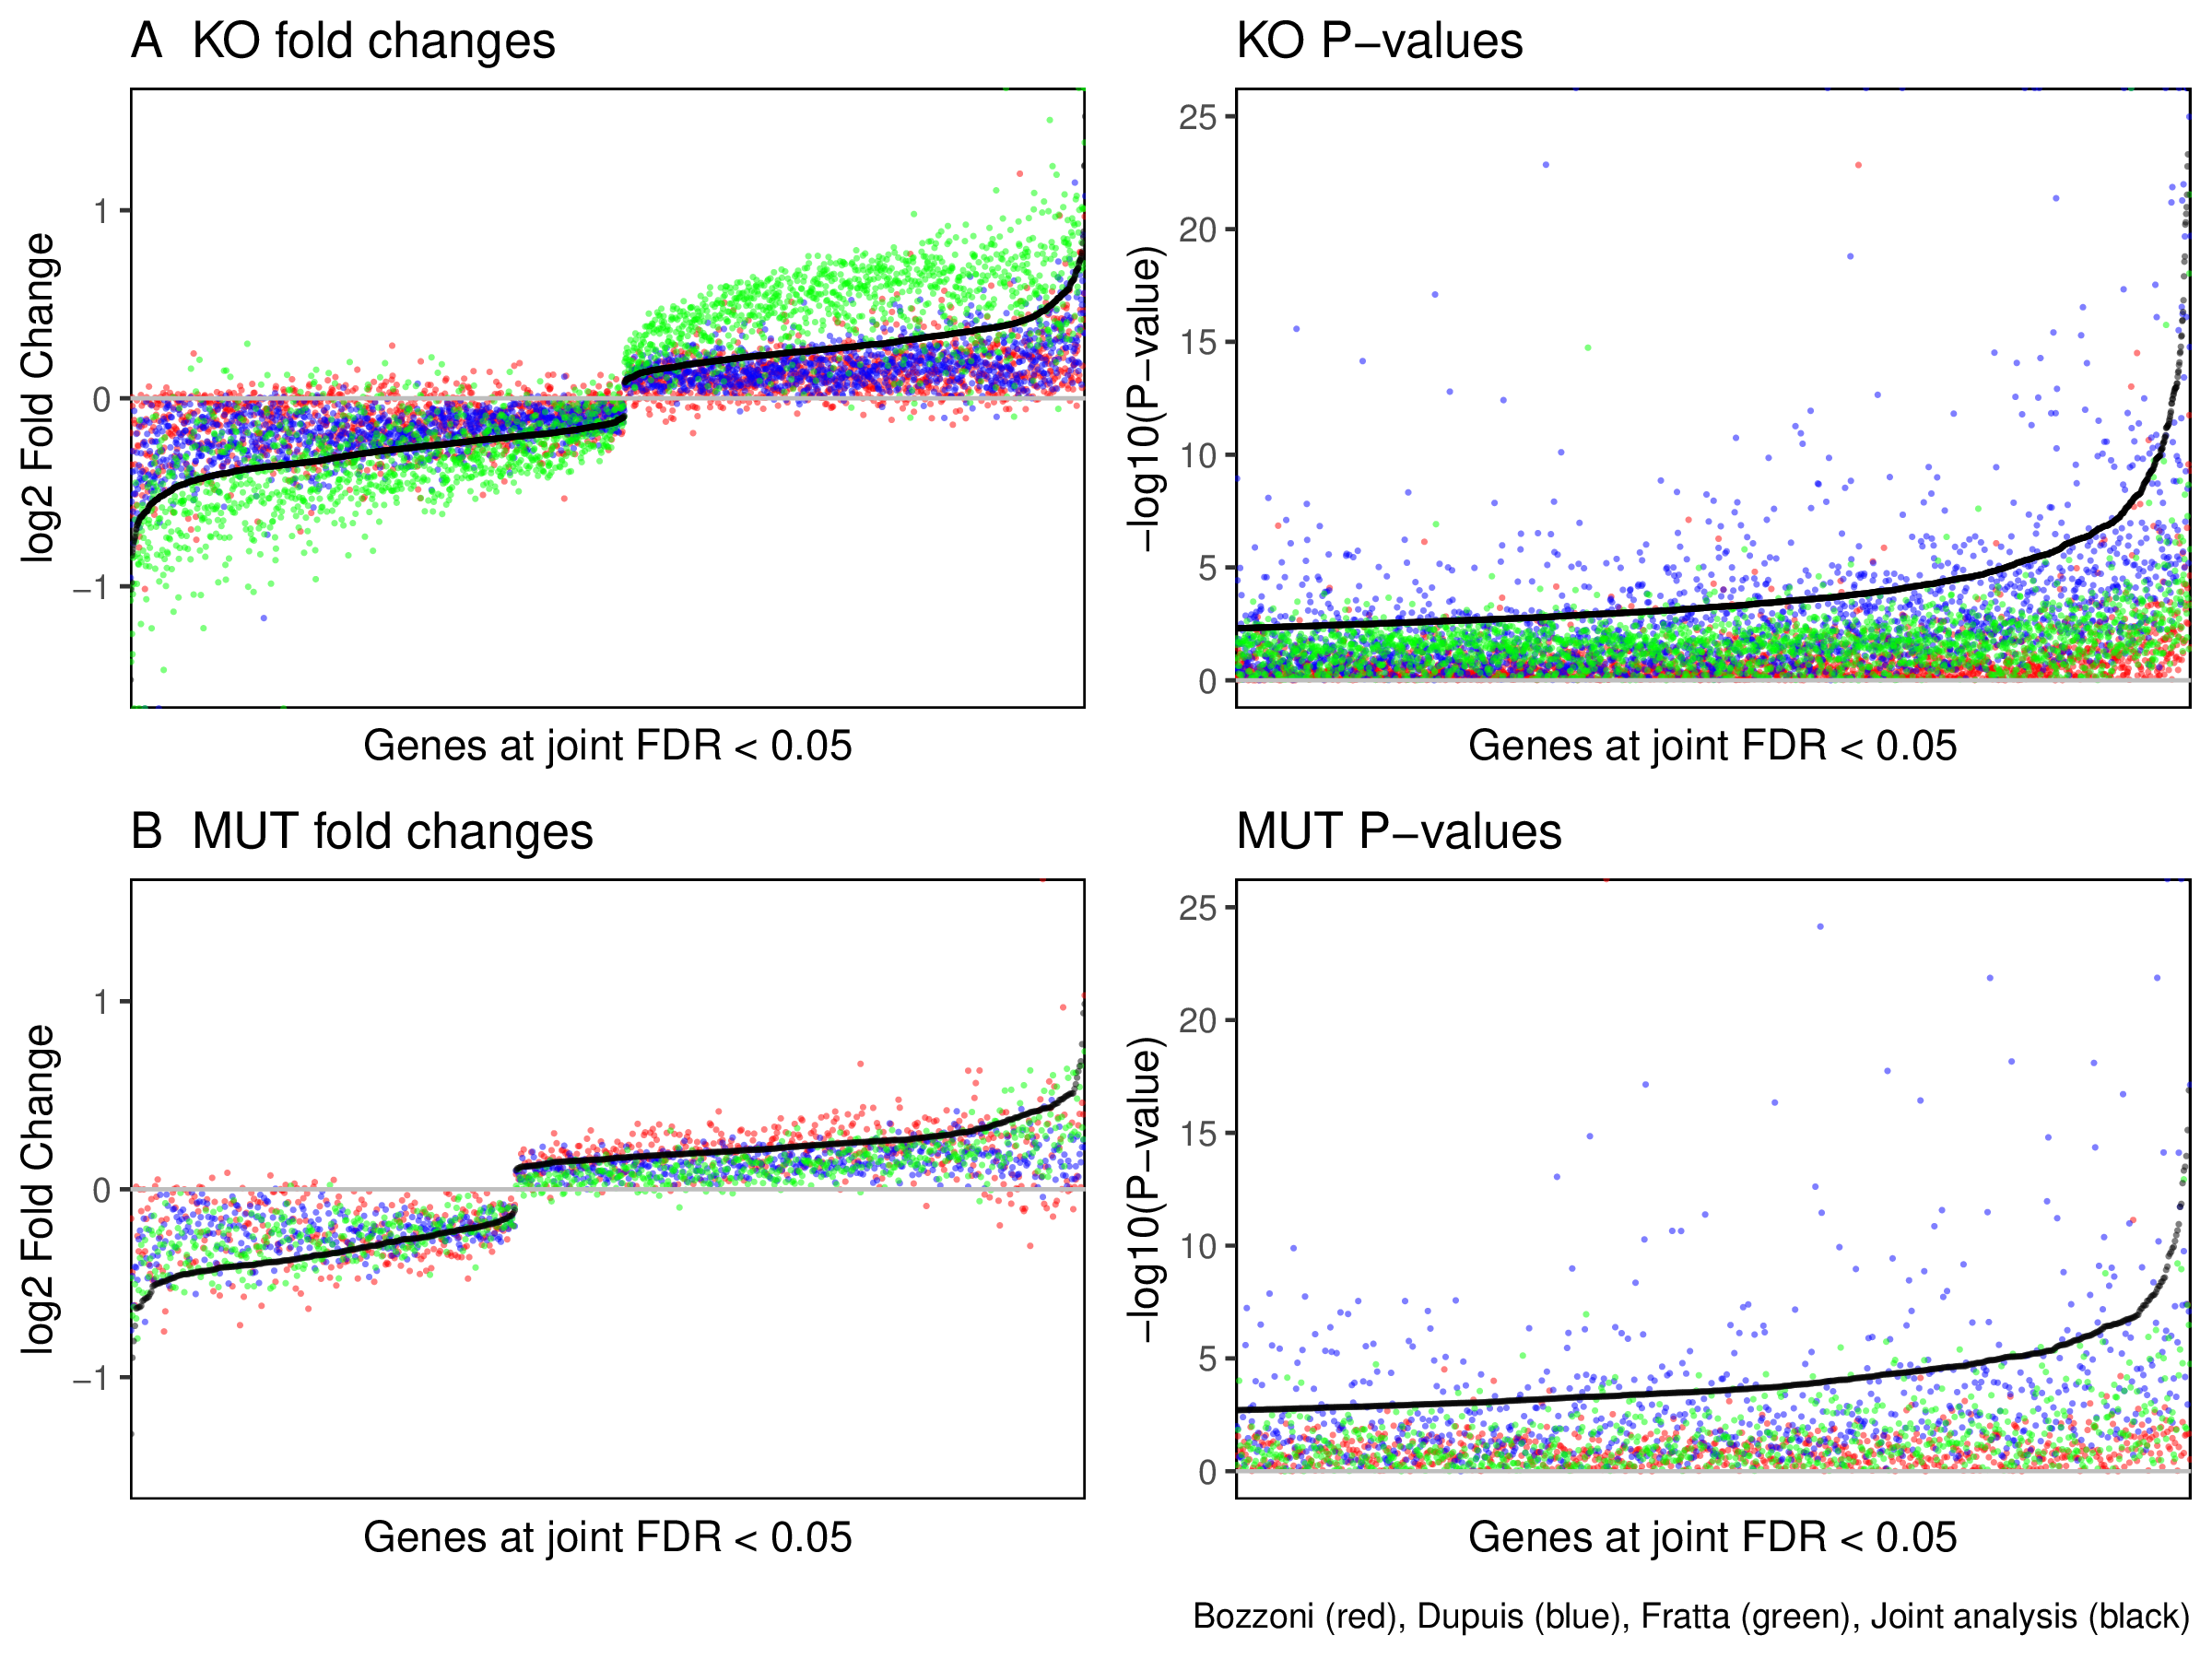
\includegraphics[width=\textwidth]{Figures/06_fus_meta/fitted_vs_individual_p_lfc.png}
	\caption[Joint differential expression increases power and adjusts effect sizes]{
		\textbf{Joint differential expression increases power and adjusts effect sizes.}
		\textbf{(A)} Plotting the $log_2$ fold changes (left) and \textit{P}-values (right) for the 2136 KO genes and 754 MUT genes found at FDR < 0.05 in the two joint analyses. Values found in the individual analyses, Bozzoni (red), Dupuis(blue) and Fratta (green) are compared to the value produced by the joint analysis (black).
		\textbf{(B)} As before but for the MUT analyses.
	}
	\label{fig:value_comparison}
\end{figure}

For each gene the resulting joint $log_2$ fold change and \textit{P}-value is an estimated combination of the three datasets.
I compared the values found by the individual analyses with the joint models(Fig. \ref{fig:value_comparison}).
For the KO models, the Fratta knockout comparison has larger $log_2$ fold change values for the same genes when compared to Bozzoni and Dupuis knockouts. 
The fitted $log_2$ fold change is a compromise between the estimated fold changes of all three datasets. 
When inspecting the distribution of \textit{P}-values, the Dupuis KO dataset has a excess of low \textit{P}-values compared to the other two.
Therefore the joint modelling strategy increases the number of genes and harmonises three different datasets together into a set of high confidence differentially expressed genes.

% Explain strict and relaxed overlap

\begin{figure}[ht!]
	\centering
	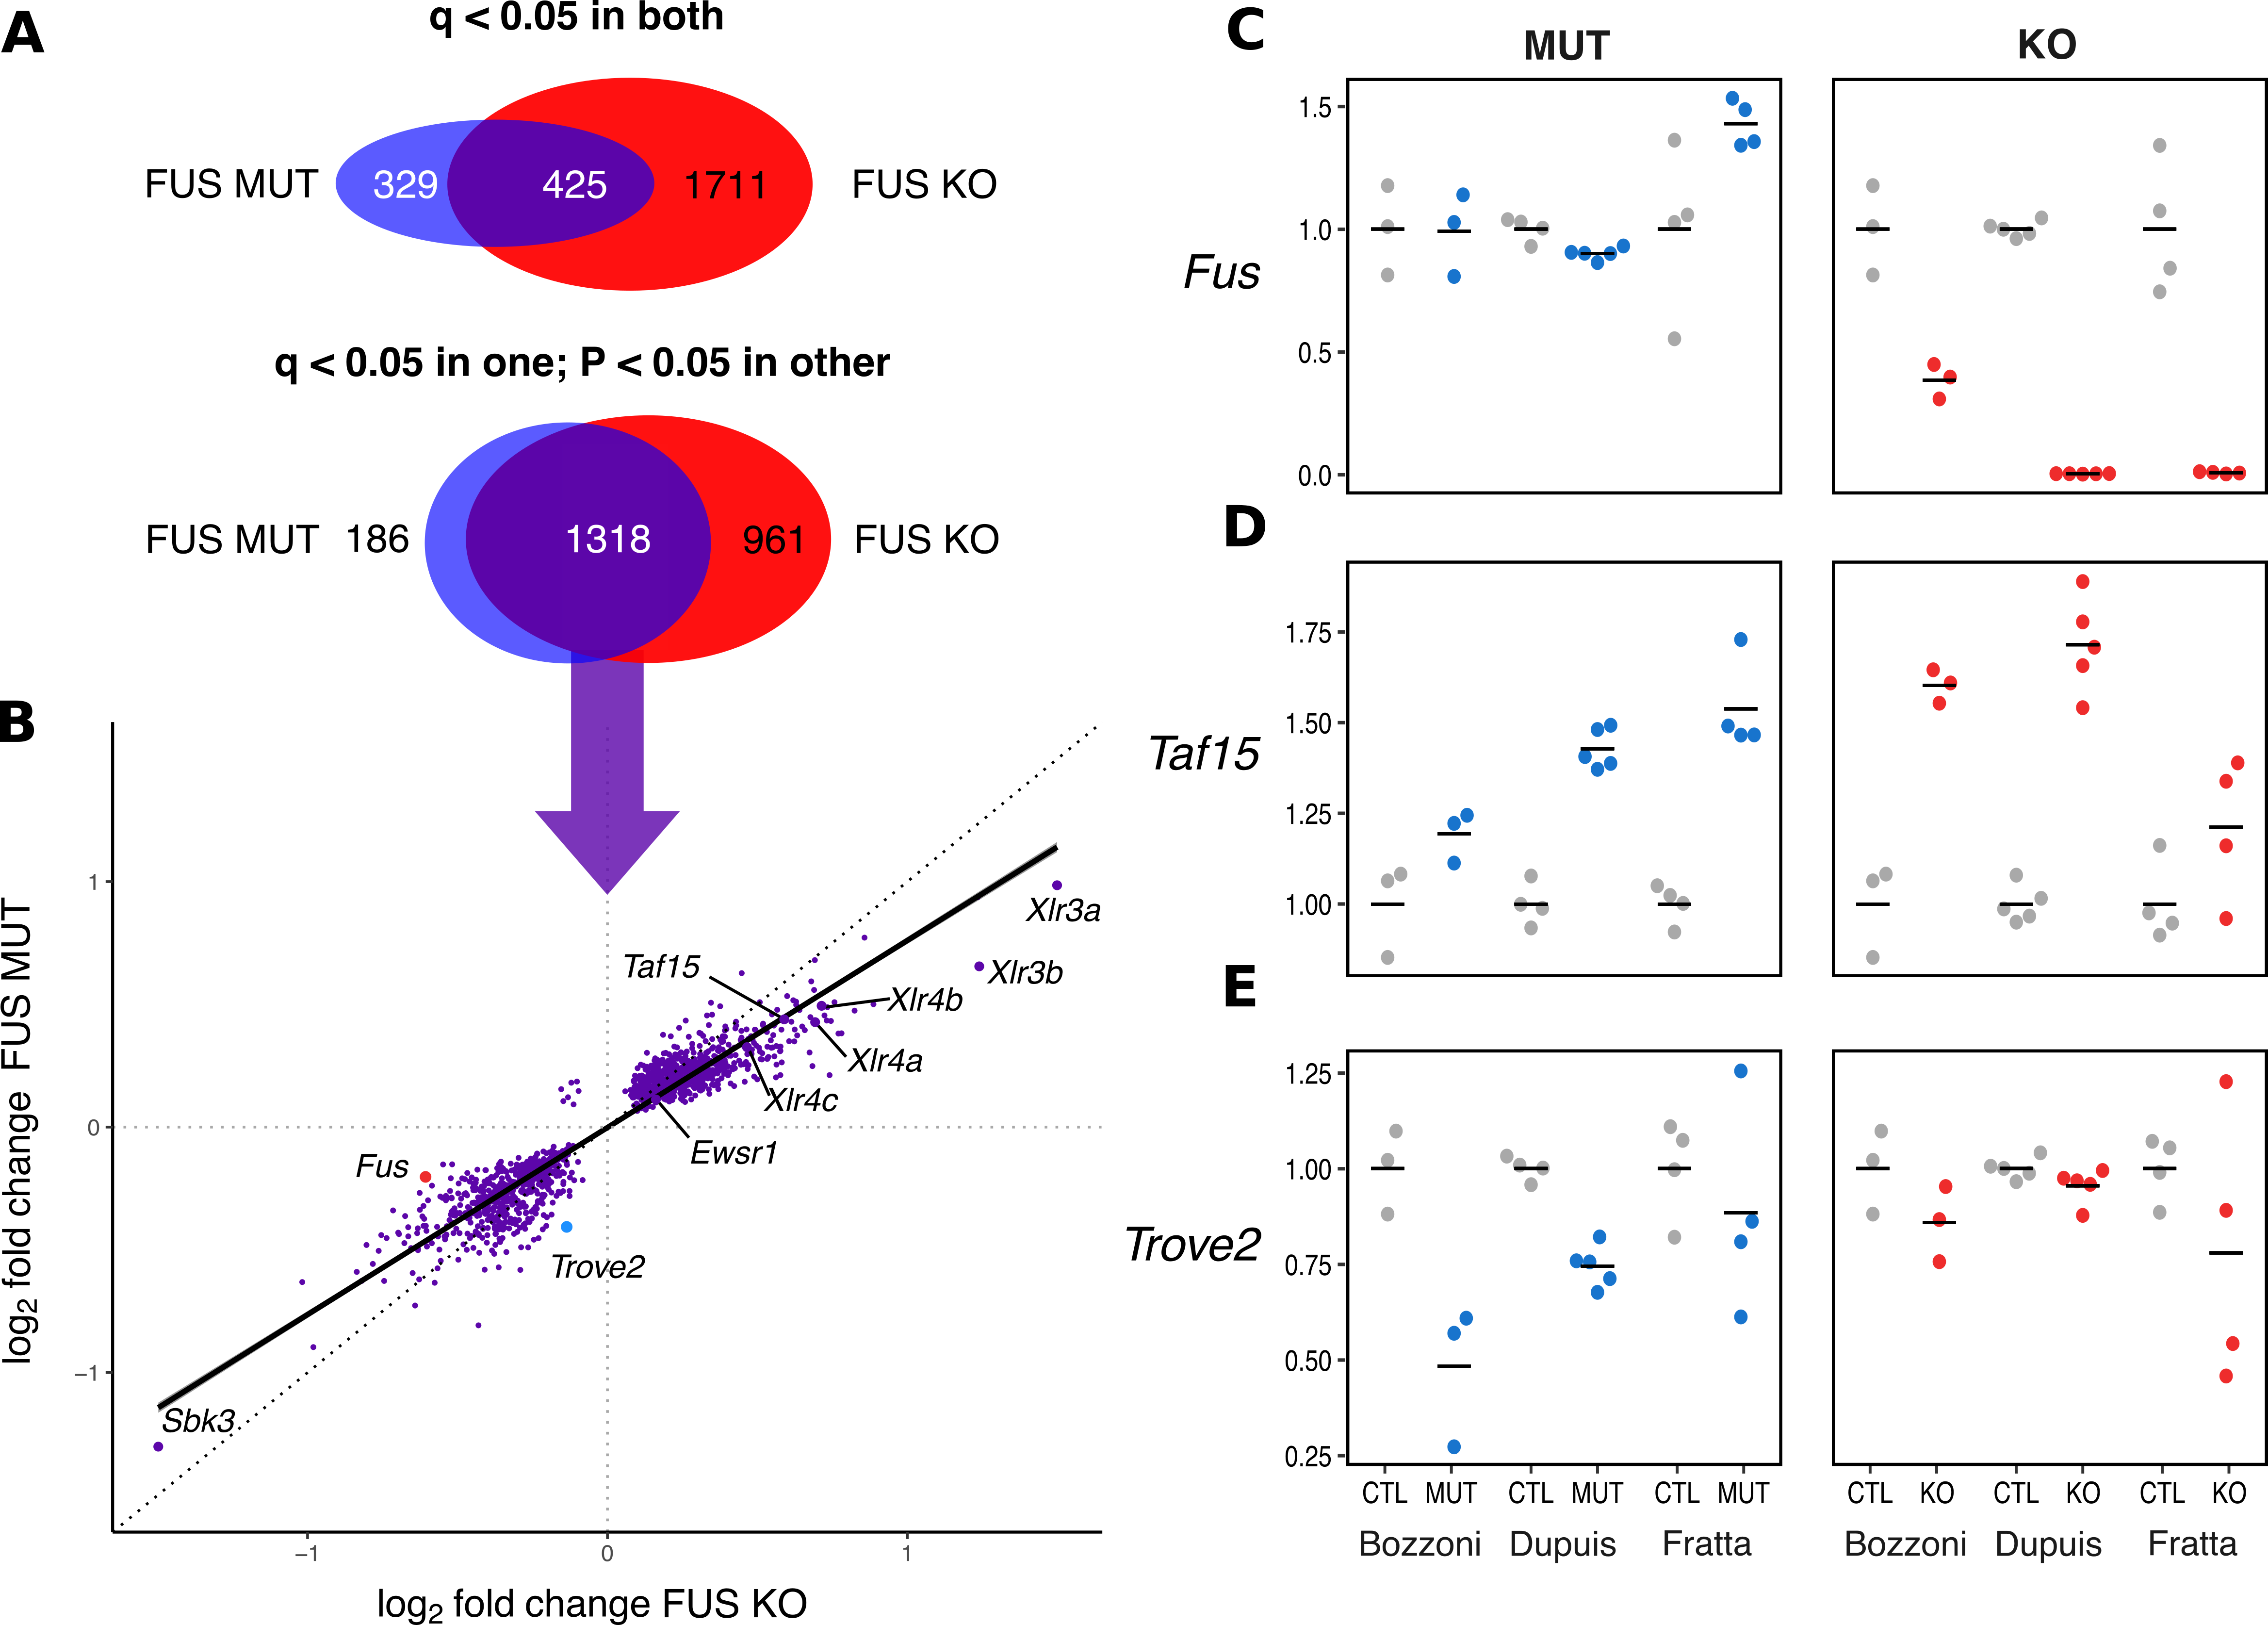
\includegraphics[width=\textwidth]{Figures/06_fus_meta/expression_multi.png}
		\caption[Overlapping the joint differential expression models shows that FUS mutations affect gene expression in generally the same direction]{
		\textbf{Overlapping the joint differential expression models shows that FUS mutations affect gene expression in generally the same direction.}
		\textbf{(A)} Venn diagrams show the overlap between the FUS KO and FUS MUT joint differential expression models with a strict FDR cut-off (upper) and a more relaxed \textit{P}-value cut-off. 
		\textbf{(B)} Plotting the fitted $log_2$ fold-change values for each of the 1318 overlapping genes in KO and MUT shows a bias towards weaker changes in MUT compared to KO.
		\textbf{(C, D,E)}: Normalised read counts in each dataset for \textit{Fus}, \textit{Taf15} and \textit{Trove2}. Samples are plotted relative to the mean expression in controls (CTL).
	}
	\label{fig:fus_expression_multipanel}
\end{figure}

The joint models provide two set of genes where we can be confident of a shared signal between the three datasets.  
I next looked for evidence of a shared gene expression signal between the KO model and the MUT model.
%If there truly is a cytoplasmic gain of FUS function on gene expression then I would expect to see a set of genes specific to NLS mutation or a set of overlapping genes that change in opposing directions.
I first used a conservative threshold for overlap, where a gene must be significant at FDR < 0.05 in both models. 
This produced an overlap of 425 shared genes between KO and MUT (Fig. \ref{fig:fus_expression_multipanel}A), with 329 mutation-specific genes and 1711 knockout specific genes.
I next used  a relaxed overlap criteria where a gene overlaps if it reaches FDR < 0.05 in one model and an uncorrected P < 0.05 in the other.
This increased the overlap to 1318 genes, reducing the specific genes to 186 in the MUT model, and 961 in KO.
The majority of genes are now shared between the two models. 


% comparing directions in the overlapping genes
Comparing the log$_2$ fold changes found for the 1318 overlapping genes between FUS KO and FUS MUT showed that only 7 genes are altered in opposing directions (Fig. \ref{fig:fus_expression_multipanel}B) .
Fitting a linear model between the fold changes of the two datasets shows that the effect of FUS MUT on gene expression is 76\% that of FUS KO.  ($\beta$ = 0.76; P < 1e-16 F-test; $R^2$ = 0.90).
This suggests that while FUS KO and FUS MUT affect the same genes in the same directions, the magnitude of change is greater in FUS KO than FUS MUT. 
This relationship is not an artefact of the relaxed overlap criteria as fitting the model on just the 425 strictly overlapping genes resulted in $\beta = 0.8; P < 1e-16$. % R^2?
The relative weakness of NLS mutations compared to knockouts can be explained as NLS mutant FUS can still be detected in the nucleus at low levels \citep{Devoy2017, Scekic-zahirovic2016}.
%Therefore the overlapping genes are the result of nuclear loss of FUS.

% individual hits
Visualising individual genes in all the datasets demonstrates the power of the joint models.
%It also clearly shows the higher within-condition variance in the Fratta dataset compared to the Dupuis dataset.
\textit{Fus} itself is unchanged in the FUS MUT joint model  but strongly downregulated in FUS KO (Fig. \ref{fig:fus_expression_multipanel}C).
The Bozzoni knockout  is weaker than the one used by Dupuis and Fratta, with a reduction of \textit{Fus} RNA to only 40\% of wildtype, compared to near 100\% knockout in the other two datasets.
The three NLS mutations are inconsistent for \textit{Fus} expression.
In Bozzoni it is unchanged, in Dupuis it is slightly downregulated (presumably due to a loss of reads covering the final exon and in Fratta it is slightly upregulated.


The other members of the FET family of RNA-binding proteins,  \textit{Taf15} and \textit{Ewsr1} have been shown to reciprocally interact with FUS at the protein and RNA level \citep{Kapeli2016,Lagier-Tourenne2012}.
\textit{Taf15} is strongly upregulated in both MUT and KO (Fig. \ref{fig:fus_expression_multipanel}D), as is \textit{Ewsr1}.  \textit{Taf15} upregulation has been repeatedly observed and validated \citep{Kino2015, Scekic-zahirovic2016}. % other citations too.
The \textit{Trove2} gene encoding the 60 kDa SS-A/Ro ribonucleoprotein,  is downregulated in MUT only and unchanged in KO (Fig. \ref{fig:fus_expression_multipanel}E) and has also been validated \citep{Scekic-zahirovic2016}.

The X-linked lymphocyte receptor genes, \textit{Xlr3a, Xlr3b, Xlr4a} and \textit{Xlr4b} are all strongly upregulated in both conditions but more so in KO than MUT. 
These genes form a cluster of paralogous genes on the X chromosome and are paternally imprinted in mice \citep{Raefski2005}.
They appear to be specific to mice.
\textit{Xlr4b} overexpression has been shown to alter dendritic spine growth in mouse neurons \citep{Cubelos2010}. 
Although these changes have been observed in another FUS knockout mouse model \citep{Kino2015},they are potentially artefacts from an imbalance of sexes between conditions. 
Embryonic mice are not typically sexed but I was able to sex the samples \textit{in silico} using the read counts aligning to Y chromosome genes (see Appendices). 
Although there is an imbalance between sexes it is clearly not driving the large upregulation of \textit{Xlr} genes. 
The upregulation of \textit{Xlr3a} is strongest within the all-male Bozzoni dataset (Fig. \ref{fig:fus_xlr_expression}A) and can also be seen in the mixed-sex Dupuis and Fratta datasets. 

\begin{figure}[ht!]
	\centering
	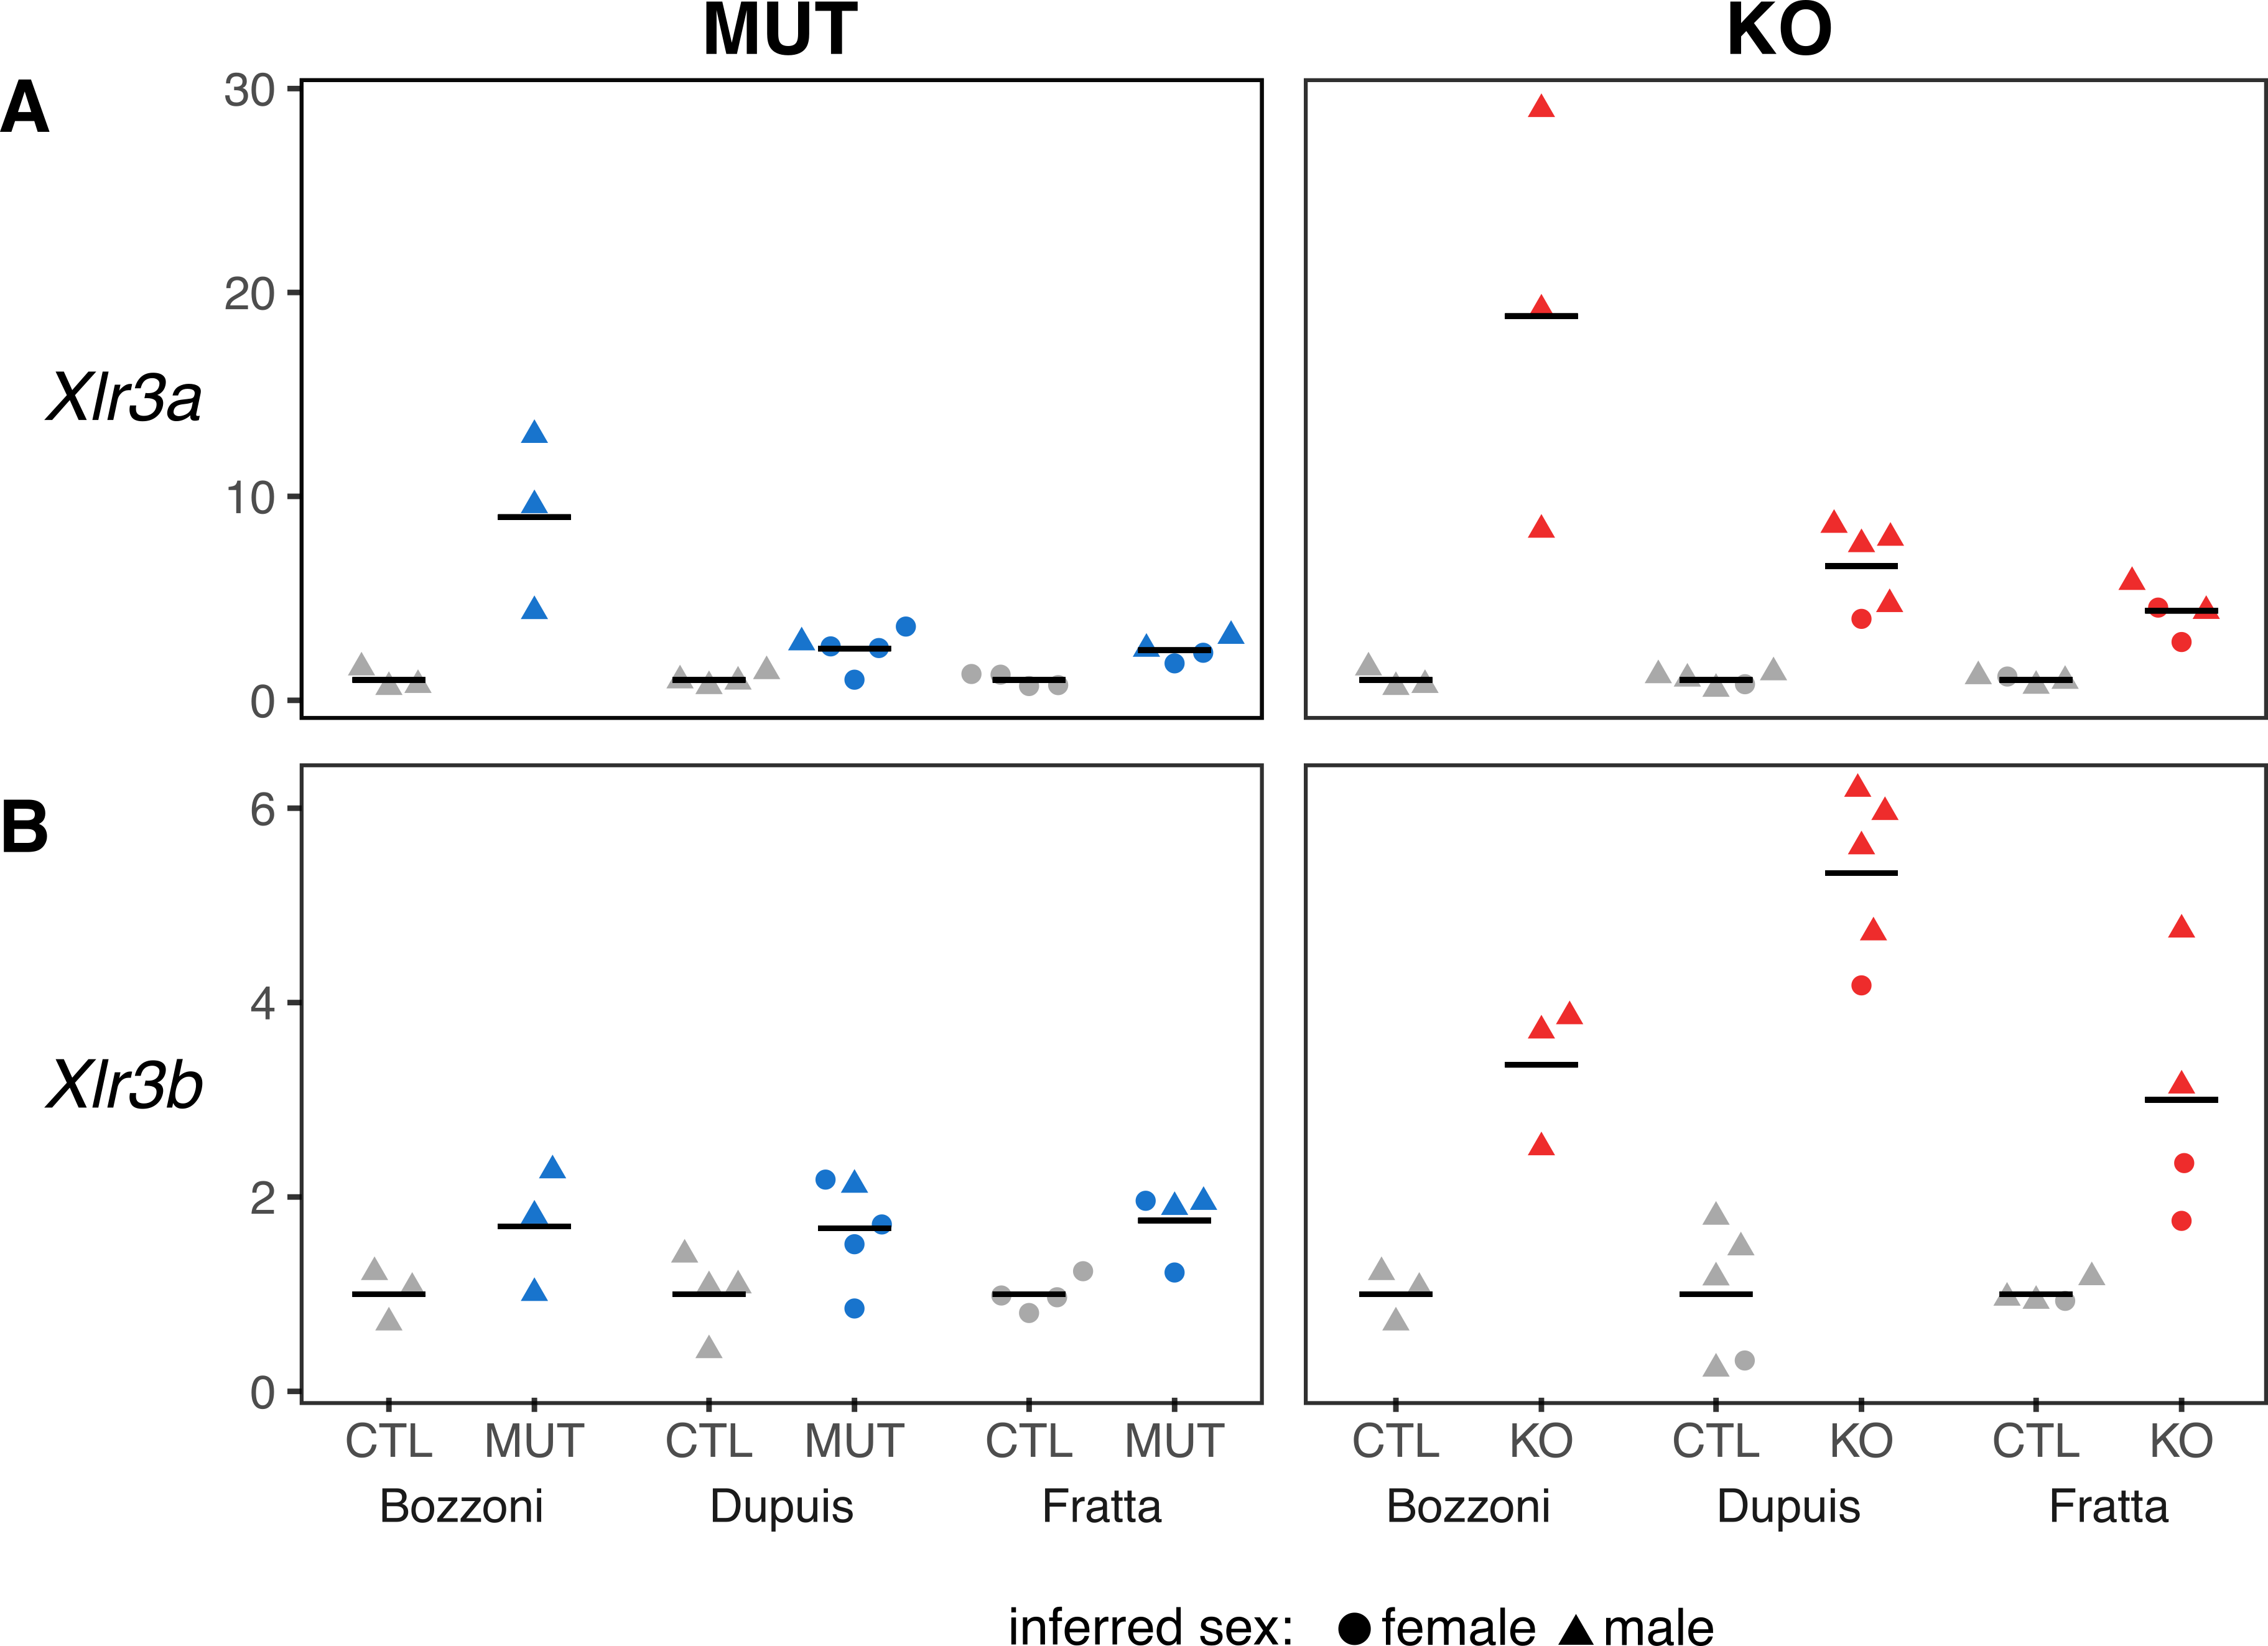
\includegraphics[width=10cm]{Figures/06_fus_meta/xlr_sex_expression.png}
	\caption[Xlr genes are upregulated in both FUS KO and FUS MUT in mice of both sexes]{
		\textbf{Xlr genes are upregulated in both FUS KO and FUS MUT in mice of both sexes}.
    	Normalised read counts in each dataset, plotted relative to the mean of each dataset and condition-specific control group for \textit{Xlr3a} \textbf{(A)} and \textit{Xlr3b} \textbf{(B)}. 
	}
	\label{fig:fus_xlr_expression}
\end{figure}



% opposing 7 genes
%Only 7 genes are changed in the opposite direction (0.5%). 3/7 have FUS iCLIP peaks overlapping
%Prickle2 is a synaptic gene, large number of iCLIP peaks in first 250kb intron - long gene!
%Dcaf7 has a 7 read iCLIP peak in the first intron (short intron)
%Cds2 has 2 peaks (7 and 1) in the 3\'\ UTR


\subsection{Synaptic and RNA-binding genes are a common gene expression response to FUS nuclear depletion}

\begin{figure}[h!]
	\centering
	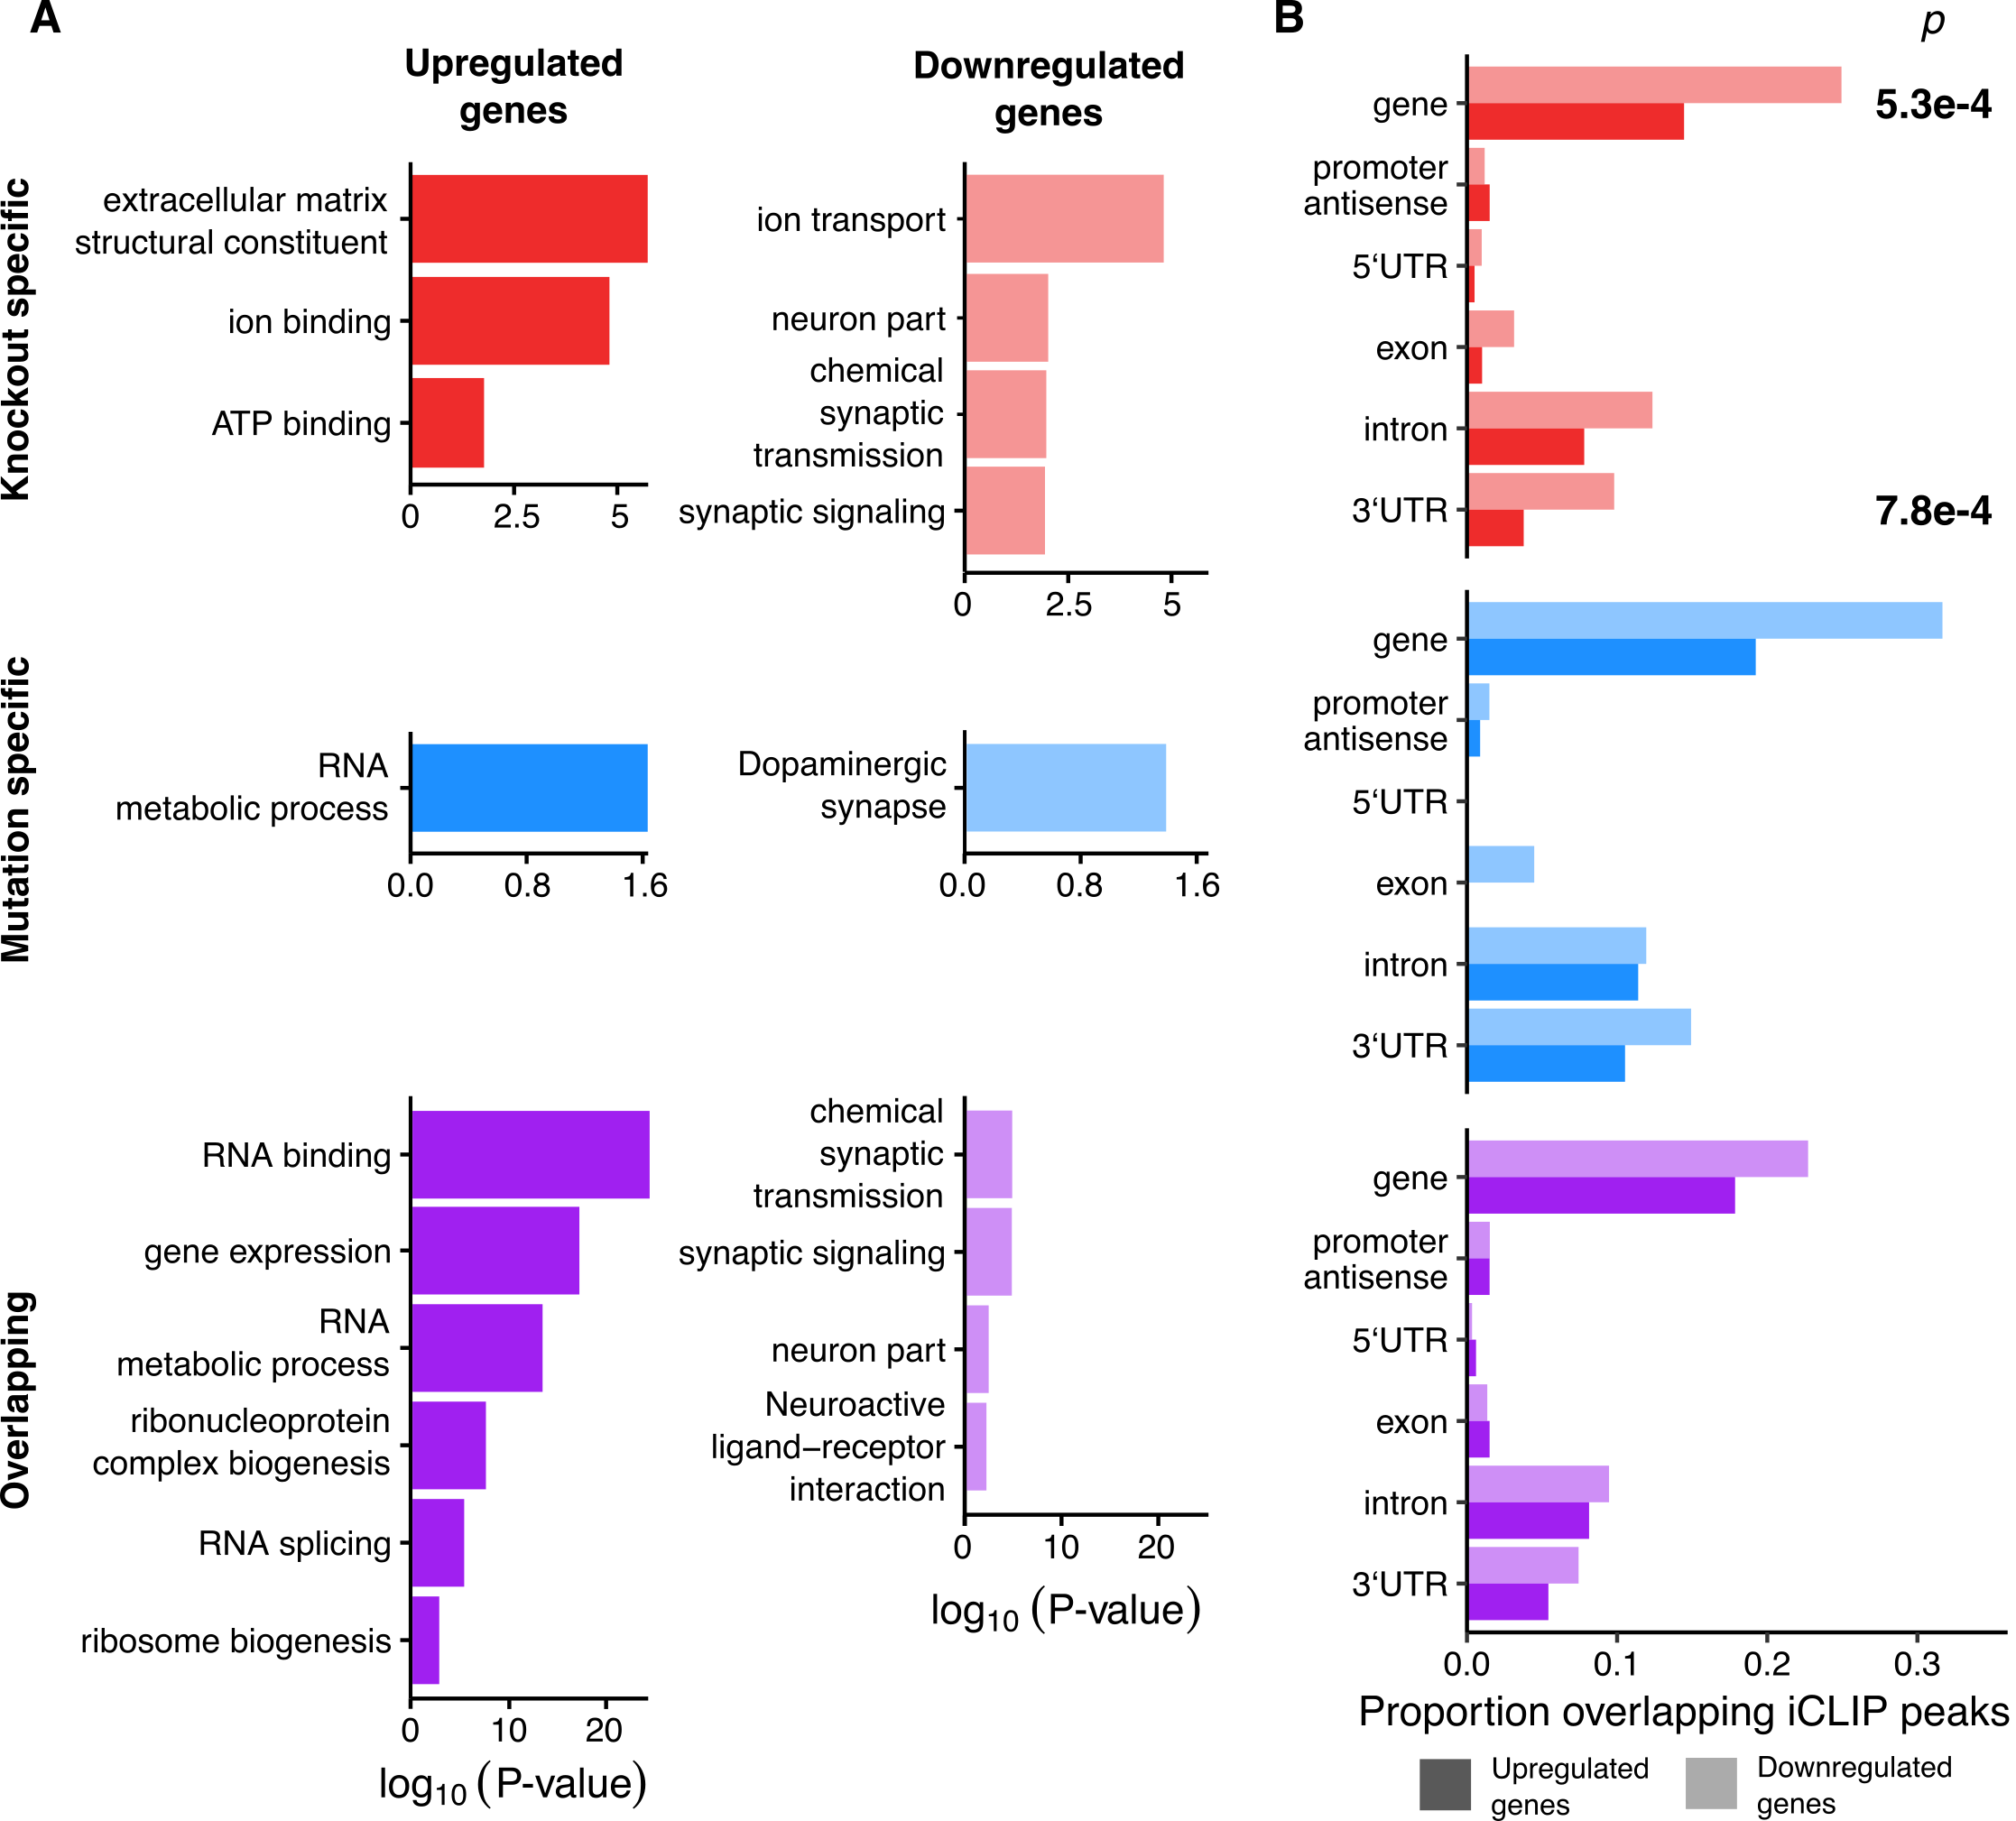
\includegraphics[width=\textwidth]{Figures/06_fus_meta/expression_curated_go_terms.png}
	\caption[Overlapping genes are enriched in neuronal and RNA terms]{
		\textbf{Overlapping genes are enriched in neuronal and RNA terms}.
		\textbf{(A)} Enriched Gene Ontology terms in the three groups of genes, split by direction.
		\textbf{(B)} Proportions of each set of genes that have any iCLIP clusters within the entire gene or in any particular gene feature, split by direction. 
		\textit{P}-values are from $\chi^2$ test of equal proportions. \textit{P}-values presented are those below the Bonferroni threshold.
	}
	\label{fig:fus_expression_go}
\end{figure}


Gene ontology (GO) terms enriched in the overlapping genes were strongly direction specific, with upregulated genes enriched in terms involving RNA binding, splicing and metabolism whereas downregulated genes were enriched in synaptic and neuronal terms (Fig. \ref{fig:fus_expression_go}A).
Knockout-specific and mutation-specific genes were less clearly enriched in specific functions. 
Knockout specific genes were involved in extracellular membrane functions, ion channels and amino acid transport whereas the mutant specific genes showed an enrichment in dopaminergic synapses and RNA metabolism.


\subsection{ Overlapping genes are bound by FUS in introns and 3\'\ UTRs}

Individual nucleotide resolution crosslinking and immunopreciation (iCLIP) is an experimental technique for identifying the RNA targets of RNA-binding proteins. 
Using iCLIP and other RNA-protein interaction techniques, FUS has been shown to preferentially bind within introns and 3\' untranslated regions (3\'\ UTRs) rather than exons. \citep{Lagier-Tourenne2012-wa, Rogelj2012, Ishigaki2012, Masuda2015, Kapeli2016}. 
FUS binding at the 3\'\ UTR has been shown to influence polyadenylation of certain genes \citep{Masuda2015} but may also have a role in directing mRNA localisation or competing with microRNAs, which in animals predominantly bind 3\'\ UTR sequences to trigger degradation \citep{Lee1993,Carthew2009}.
A small number of genes have been reported to have FUS binding  sites upstream and antisense of the promoter, which correlated with upregulation of the gene upon FUS knockdown \citep{Ishigaki2012}.
I used the coordinates of FUS binding sites enriched relative to a background control in a published FUS iCLIP dataset from embryonic day 18 mouse brain \citep{Rogelj2012} to investigate a relationship between specific FUS binding and the direction of gene expression in the different gene sets.

The iCLIP binding profiles of the three sets of genes are similar with introns and 3`UTR sequences most commonly bound (Fig. \ref{fig:fus_expression_go}B).  
Comparing the proportion of upregulated and downregulated genes that change only in FUS knockout, there is an enrichment in iCLIP clusters in downregulated genes (\textit{P}=5.3e-4, $\chi^2$ test of equal proportions), an enrichment driven primarily by 3\'\ UTR binding (\textit{P}=7.8e-4). 
This direction preference is not seen in the mutation-specific or overlapping gene sets.
Promoter-antisense binding is found in a small number of genes and at a similar proportion between gene set and direction of change.
As the iCLIP used is from predominantly nuclear wildtype FUS, any potential cytoplasmic interactions between NLS mutant FUS and spliced mRNAs cannot be observed.

% wrap up gene expression?

%% SPLICING

\subsection{FUS modulates the inclusion of a set of highly conserved RNA-binding protein introns}

I then used the same joint modelling approach to assess evidence of differing effects between FUS knockout and NLS mutation on alternative splicing.
For the individual analyses I used SGSeq \citep{Goldstein2016} to discover and quantify all possible alternative splicing isoforms, both novel and annotated. 
The read counts supporting each splicing variant were used to test for differential usage between conditions for either NLS mutation or knockout and their respective controls.
For the joint analyses, I ran SGSeq on all the samples simultaneously and then fit two separate models for all knockout samples and their controls (KO) and all mutation samples and their controls (MUT), incorporating a dataset-specific covariate. 
Models were fit using DEXSeq \citep{Anders2012}.
Table \ref{tab:splicing_results} summarises the numbers of splicing events in the KO and MUT models at FDR < 0.05.
%Here the weakness of the Dupuis samples for capturing splicing is revealed, presumably due to the short single-end sequencing reads. 
The joint models increased power as for MUT and KO respectively 93 and 890 events are found to be significantly altered, more than the sums of the individual analyses.
There is also a very good concordance between each individual analyses and their joint model, with the exception of the Bozzoni mutant samples (only 7 out of 31).

Comparing the joint FUS knockout and NLS mutation splicing models, the two overlap at both a strict and relaxed significance threshold.
With the relaxed overlap criteria only 16 splicing events remain specific to the NLS mutations (Fig. \ref{fig:fus_splicing_multi}A) .
There are 501 knockout specific splicing events and 405 that overlap between the two conditions.
Manual curation of the 16 mutant specific events gave little confidence of a mutation-specific effect on splicing, as only one splicing event appeared convincingly in all 3 datasets.
The single event that did appear to be real was an intron retention event in \textit{FUS}, far upstream of the mutated NLS region.

% TABLE OF SPLICING EVENT COUNTS
\begingroup
\renewcommand{\arraystretch}{1.5} 
\begin{table}[h]
	%\begin{centerline}
	\begin{tabular}{|r|ccc|ccc|}
		\hline
		%\centering
		& Bozzoni & Dupuis & Fratta & Bozzoni & Dupuis & Fratta\\[-0.3cm]
		& MUT & MUT & MUT & KO & KO & KO\\
		\hline
		Individual hits                & 47 & 1 & 79 & 275 & 54 & 316 \\
		Overlapping joint model & 9 & 0 & 33 & 143 & 31 & 206 \\
		Unique to dataset          & 38 & 1 & 46 & 132 & 23 & 110 \\
		\hline
		\textbf{Joint model}       & \multicolumn{3}{c|}{93} & \multicolumn{3}{c|}{890} \\
		\hline
		Overlap (strict)              & \multicolumn{2}{c|}{33} & \multicolumn{2}{c|}{\textbf{60}} & \multicolumn{2}{c|}{830} \\
		Overlap (relaxed)           & \multicolumn{2}{c|}{16} & \multicolumn{2}{c|}{\textbf{405} } & \multicolumn{2}{c|}{501} \\
		\hline
	\end{tabular}
	%\end{centerline}
	\caption[Results from separate and joint splicing analysis]{\textbf{Results from separate and joint splicing analysis}}
	\label{tab:splicing_results}
\end{table}
\endgroup

% types of splicing event - how many are annotated?
Comparing the different types of splicing event shows a similar distribution between knockout-specific and overlapping splicing events, both of which are dominated by complex splicing events.
These events are combinations of multiple types, such as a cassette exon accompanied by a retained intron and multiple alternative 3\' and 5\' splice sites, all within the same locus. 
When using tools like SGSeq that can pick up novel splicing events it can be expected that the majority of events are indeed complex. This has been seen with other splicing tools \citep{Vaquero-Garcia2016}.
An example of a complex event is in \textit{Ybx1}, which comprises a cassette exon within a retained intron  (Fig. \ref{fig:fus_splicing_multi}D).
The second largest category of event are retained introns.
An example of this class is seen in \textit{Ewsr1}, where a normally retained intron is less retained in both FUS knockout and NLS mutation (Fig. \ref{fig:fus_splicing_multi}E).
The third largest category are the cassette exons, which can either be skipped or included. 
An example is an annotated cassette exon in the neuronal gene \textit{Nrxn3}, which is included more in FUS knockout and NLS mutation when compared to wildtype (Fig. \ref{fig:fus_splicing_multi}F).
RNA-seq traces of all events mentioned above are in the appendices.
% expand on this or not?
Alternate 5\' and 3\' splice sites can be found in all three sets of genes, with alternate 5\' sites appearing at twice the rate of alternate 3\' splice sites. 
This discrepancy could be explained by the interaction of FUS with the U1 snRNP \citep{Yu2015a,Yu2015b}.
Knockdown or NLS mutation of FUS could lead to impaired U1 snRNP binding and hence disrupted 5\' splice site recognition.


\begin{figure}[t]
	\centering
	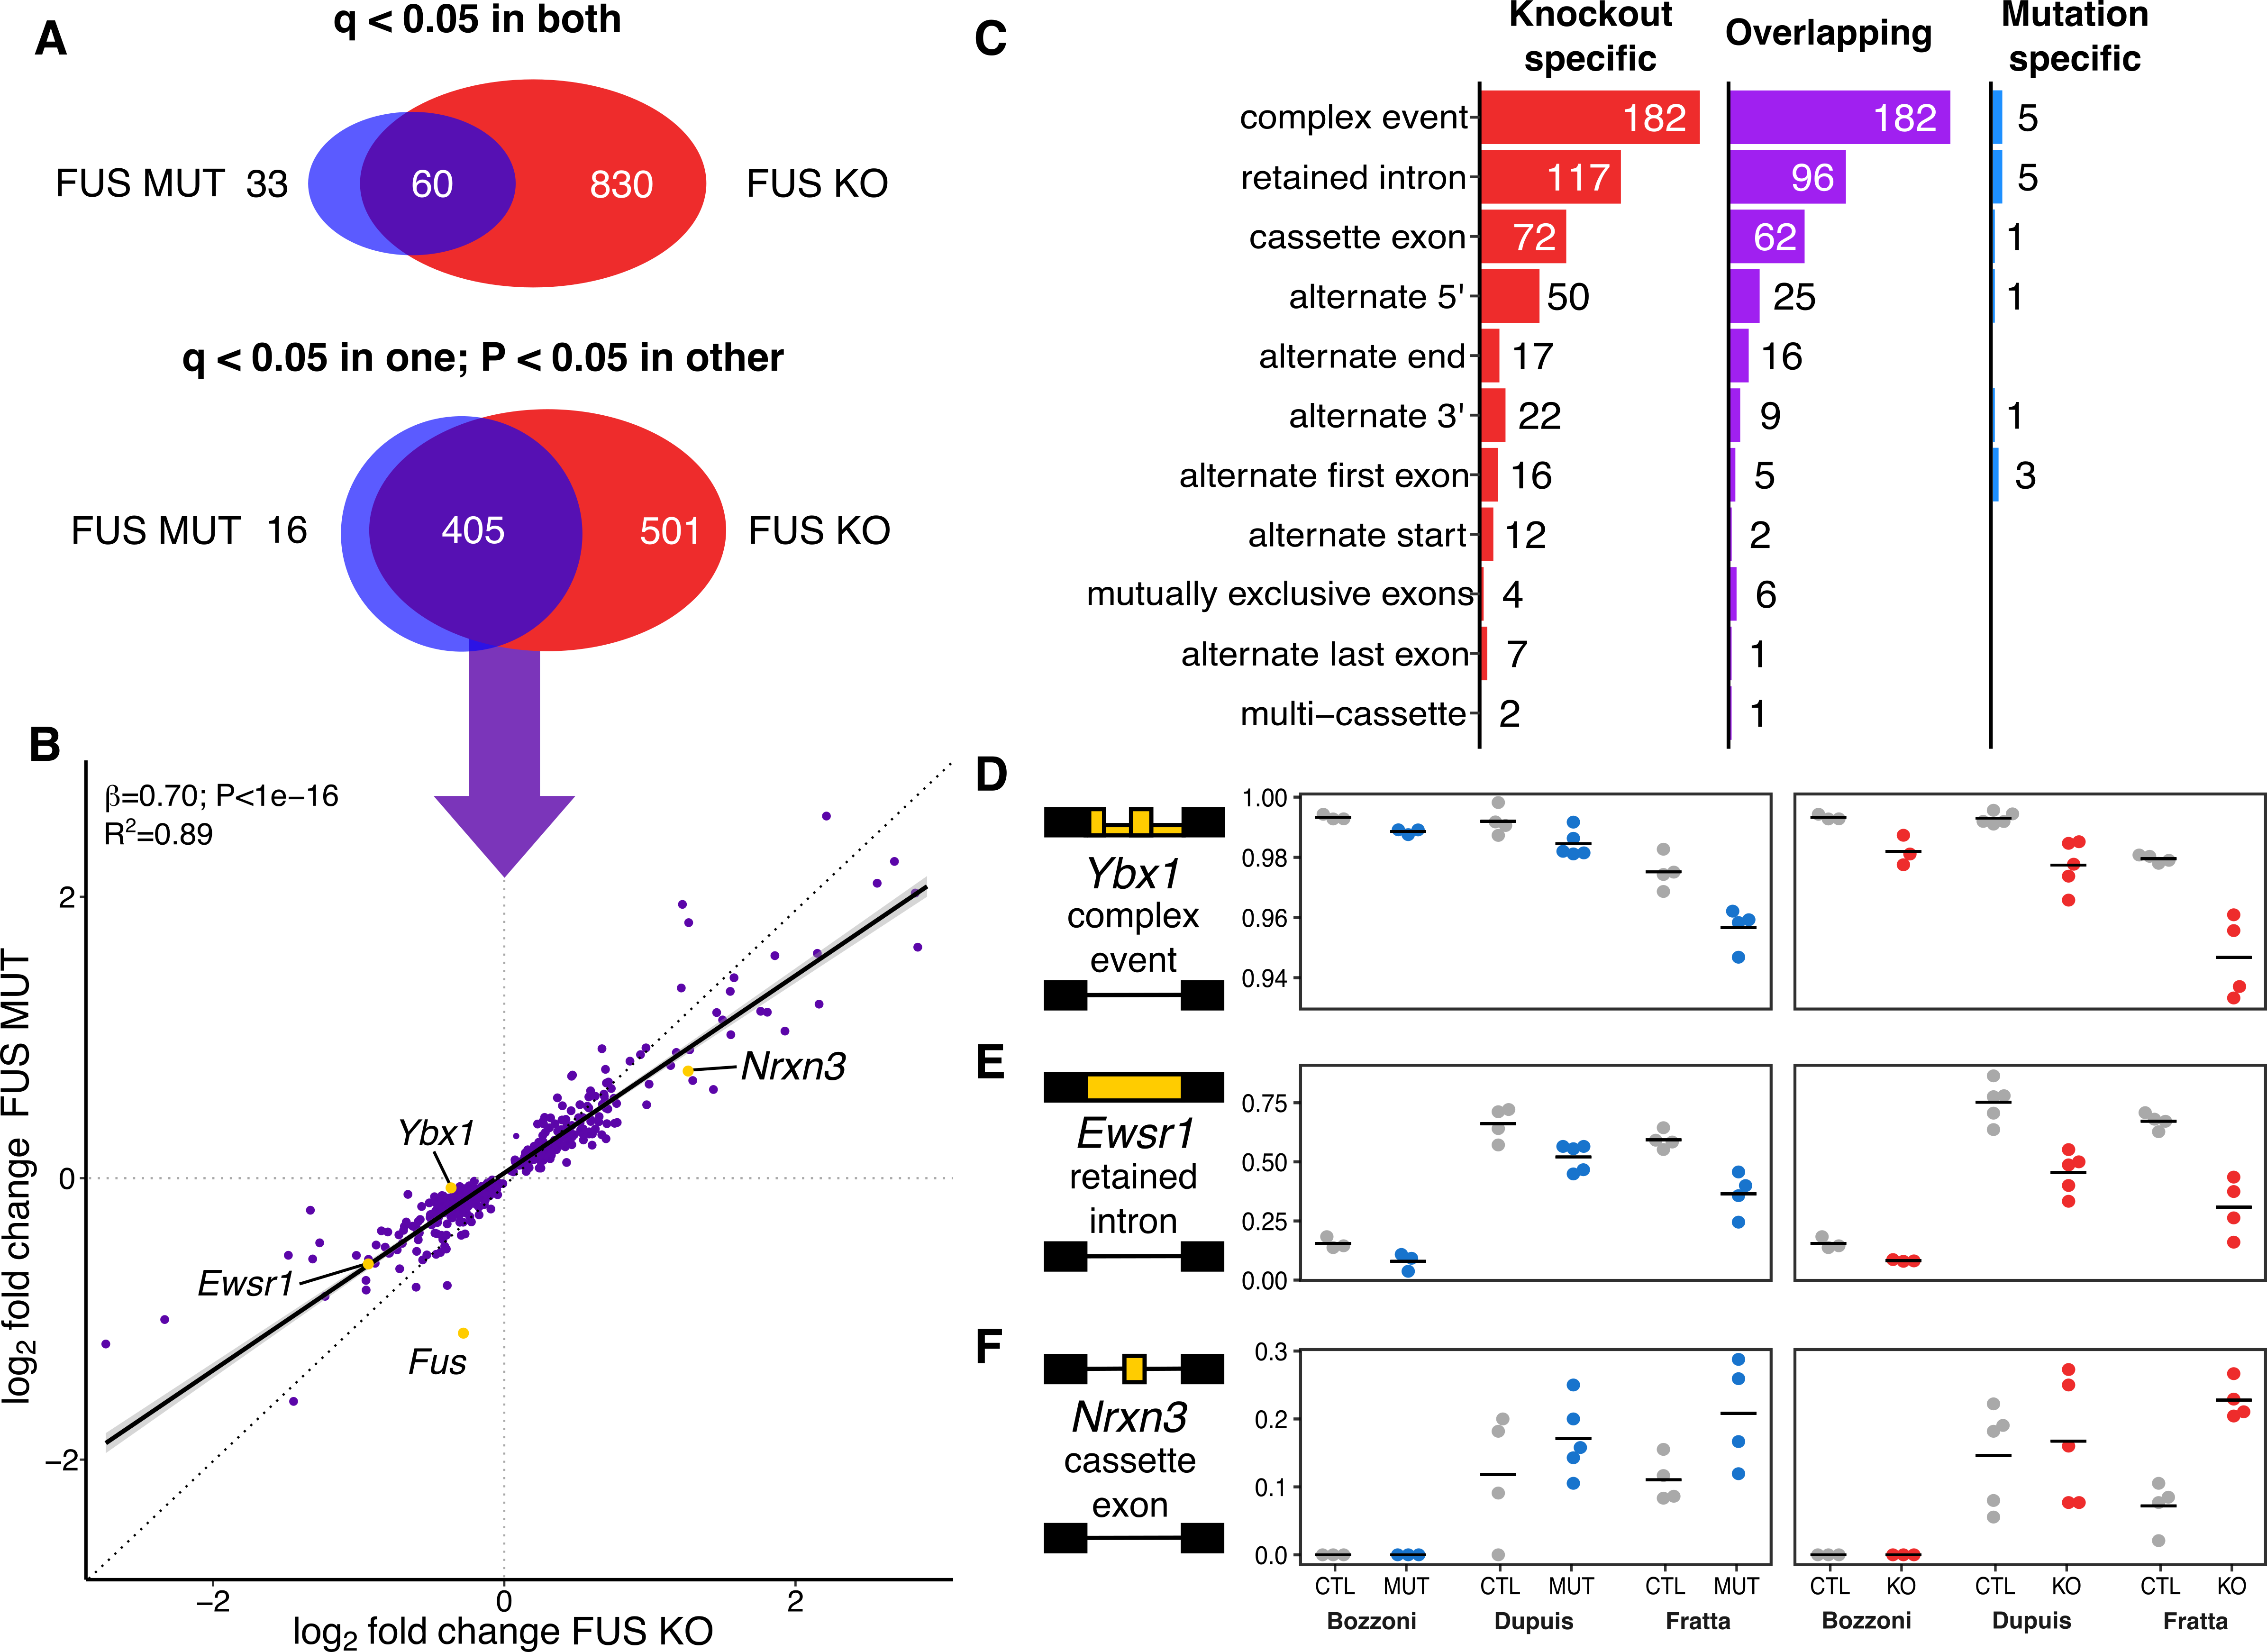
\includegraphics[width=\textwidth]{Figures/06_fus_meta/splicing_multi.png}
	\caption[Splicing changes  strongly overlap between KO and MUT joint models]{
			\textbf{Splicing changes  strongly overlap between KO and MUT joint models.}
			\textbf{(A)} Overlapping KO and MUT splicing events results in a significant overlap. The number of mutation specific events drops to just 16 when a more relaxed overlap threshold is used.
			\textbf{(B)} Splicing events plotted by their $log_2$ fold change values in the KO and MUT joint models. There is a bias towards larger changes in the KO than MUT ($\beta = 0.7$; .P < 1e-16). Dotted line $y=x$; bold line fitted regression
			\textbf{(C)} Categories of splicing variant found in each set of events. Complex events are defined as splicing events which are made up of multiple categories.
			\textbf{(D-F)} Examples of a cassette exon, retained intron and a complex event in all three datasets. 
	}
	\label{fig:fus_splicing_multi}
\end{figure}

Comparing the strict to the relaxed overlap criteria between the KO and MUT joint models reduces the number of events found to be specific to FUS mutation to 16, with 405 overlapping events and 501 found to be specific to FUS knockout (Table \ref{fig:fus_splicing_multi}). 
Plotting the $log_2$ fold changes of the overlapping splicing events, there is a similar trend towards larger fold changes in the KO than the MUT joint models ($\beta$ = 0.7, P < 1e-16; F-test; $R^2$ = 0.89). 
There are no overlapping splicing events that change in opposing directions between the two joint models.

\begin{figure}[t]
	\centering
	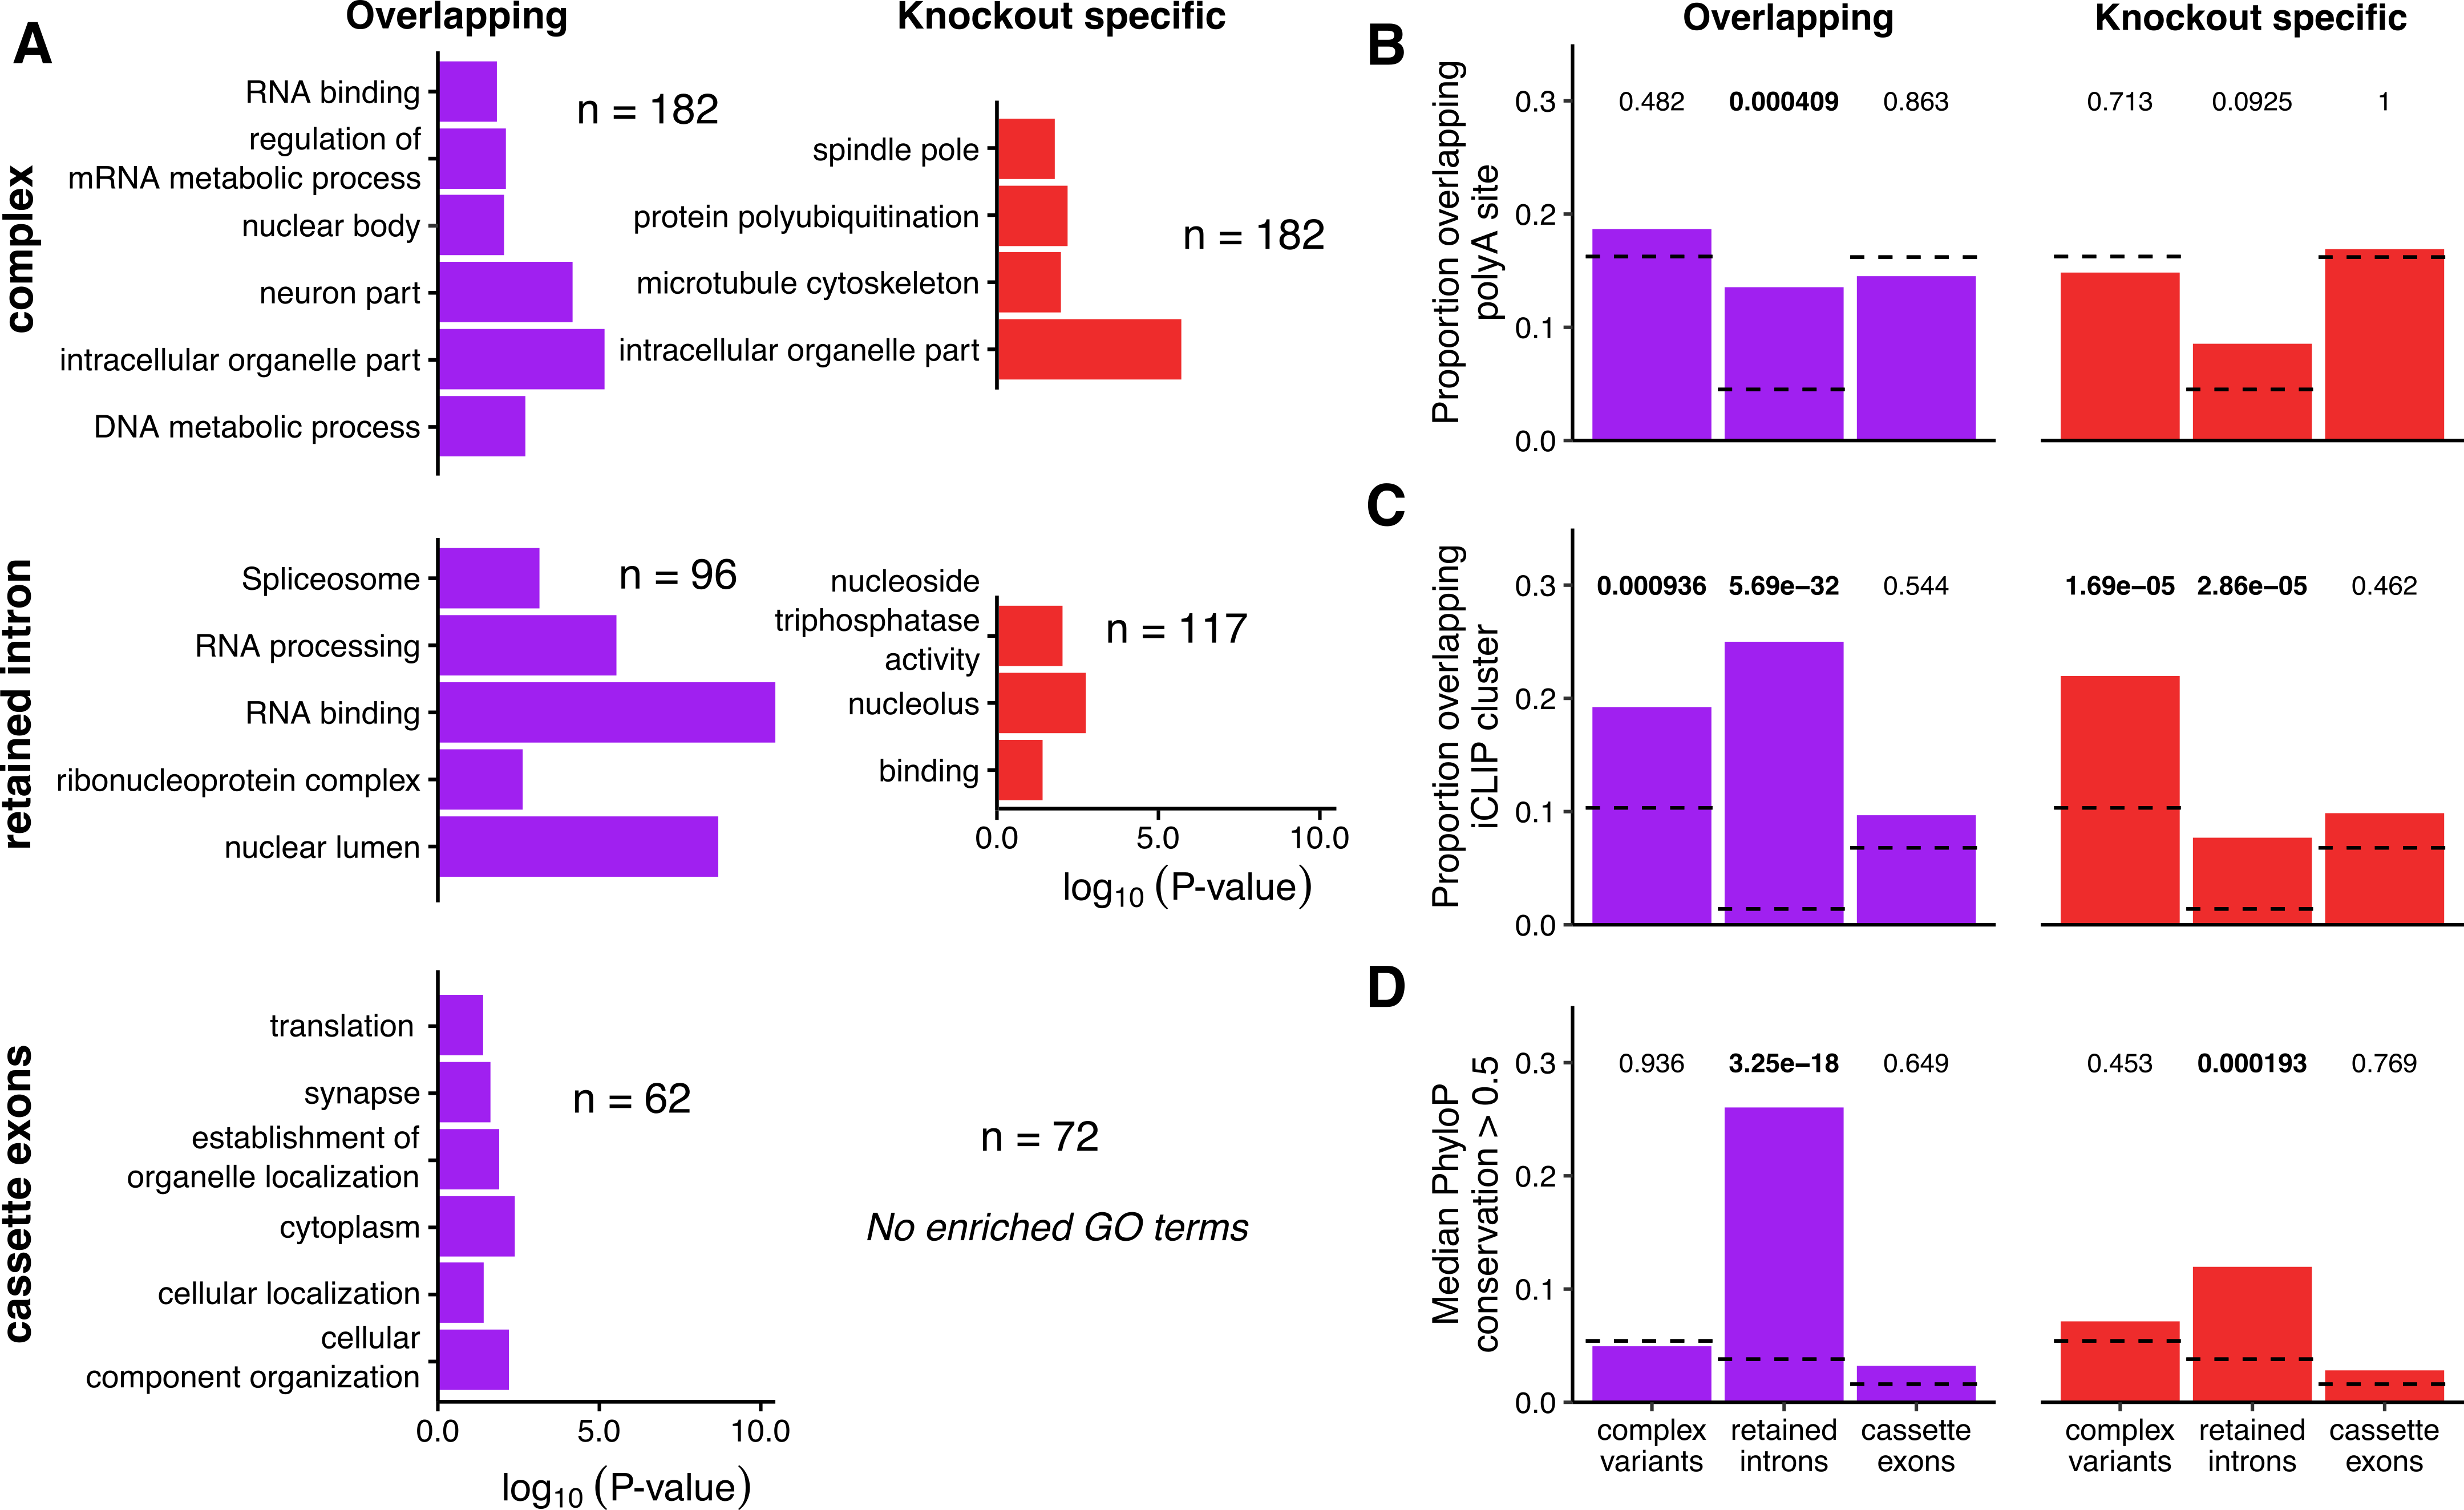
\includegraphics[width=\textwidth]{Figures/06_fus_meta/splicing_go_functions.png}
	\caption[Intron retention events are highly conserved and occur in RNA binding proteins]{
		\textbf{Intron retention events are highly conserved and occur in RNA binding proteins.} 
		\textbf{(A)} Significantly enriched Gene Ontology terms found in genes split by category and splicing variant type.
		\textbf{(B)} The proportion of each type of splicing variant in each category that overlaps a polyadenylation cleavage site.
		\textbf{(C)} The proportion of each type of splicing variant in each cateoory that overlaps a FUS iCLIP peak.
		\textbf{(D)} The proportion of each type of splicing variant in each category that have a median PhyloP conservation score greater than 0.5.
	}
	\label{fig:fus_splicing_functions}
\end{figure}

The three largest categories of splicing events for the knockout-specific and overlapping events were complex, retained intron and cassette exons. 
I subjected each category to enrichment tests both for gene ontology terms and other genomic features.
There was a clear enrichment in RNA-binding and neuronal GO terms in the overlapping splicing events, with terms relating to RNA binding dominating retained introns (Fig \ref{fig:fus_splicing_functions}A). 
Conversely neuronal terms were found in cassette exons. 
Knockout-specific splicing events were enriched for different sets of genes, including microtubule and nucleolus.

The complex and intron retention events may arise from differences in polyadenylation site usage.
FUS has been observed to modulate polyadenylation \citep{Masuda2015}.
To investigate this I compared each set of splicing events with a set of annotated polyadenylation sites \citep{Gruber2016}.
Only overlapping retained introns were enriched for polyadenylation sites (\textit{P}=0.004), suggesting some intron retention events are mislabelled 3\'\ UTRs (Fig \ref{fig:fus_splicing_functions}B).

Direct regulation of splicing events by FUS binding to introns has been proposed using RNA-protein interaction experiments \citep{Lagier-Tourenne2012,Rogelj2012, Ishigaki2012}.
To look for evidence of FUS regulating these splicing and polyadenylation events I used the same set of FUS iCLIP clusters from \citep{Rogelj2012}.
Complex events and retained introns were enriched in having iCLIP clusters within the affected introns in both overlapping and knockout-specific contexts.
The strongest enrichment was seen in overlapping retained introns (\textit{P}=5e-32; Fig \ref{fig:fus_splicing_functions}A). 
No enrichment was seen in cassette exons, suggesting that cassette exon splicing changes are not the direct result of a change in FUS binding.

RNA-binding proteins often contain intronic sequences that are very highly conserved \citep{Lareau2007} and these sequences are often used in the regulation of their translation \citep{Ni2007}.
To test whether the splicing events show high sequence conservation, I calculated the median PhyloP score using the 60-way comparison between mouse and other species for each encompassing intron \citep{Pollard2010-fj}.
Sets of events were then tested on the proportion of the set with a median phyloP score > 0.5, where a score of 0 is neutral and 1 is highly conserved.
Only retained introns were shown to be enriched in sequence conservation, and  at a greater externt for overlapping (\textit{P}=3e-18) than in knockout-specific events (\textit{P}=0.0002; Fig \ref{fig:fus_splicing_functions}D). 
For cassette exons the two flanking introns are included and so the median conservation score will reflect the conservation of those introns, even when the central cassette exon itself is highly conserved.

Taken together, these results show that nuclear loss of FUS through either knockout or NLS mutation leads to a set of splicing changes concentrated in conserved intron retention events affecting other RNA-binding proteins.
 Cassette exons do not tend to be bound by FUS beyond the null expectation and originate from less conserved introns.

% overlap splicing and gene expression
As the splicing events are enriched for similar gene ontology terms as the differentially expressed genes, I reasoned that these may affect the same group of genes.
However, only 59 differentially expressed genes are found to contain a splicing event. 
Of those 59, only 12 have FUS iCLIP binding peaks (17\%).
Those 12 genes all have either complex or retained intron events and includes the U1 splicing factor \textit{Snrnp70}, the FET protein family members \textit{Ewsr1} and \textit{Taf15}, and \textit{Fus} itself. 
This analysis shows that the role of FUS on gene expression and splicing mostly affects mutually exclusive sets of genes.


\subsection{FUS autoregulation is dependent on intron retention}

\begin{figure}[h!]
	\centering
	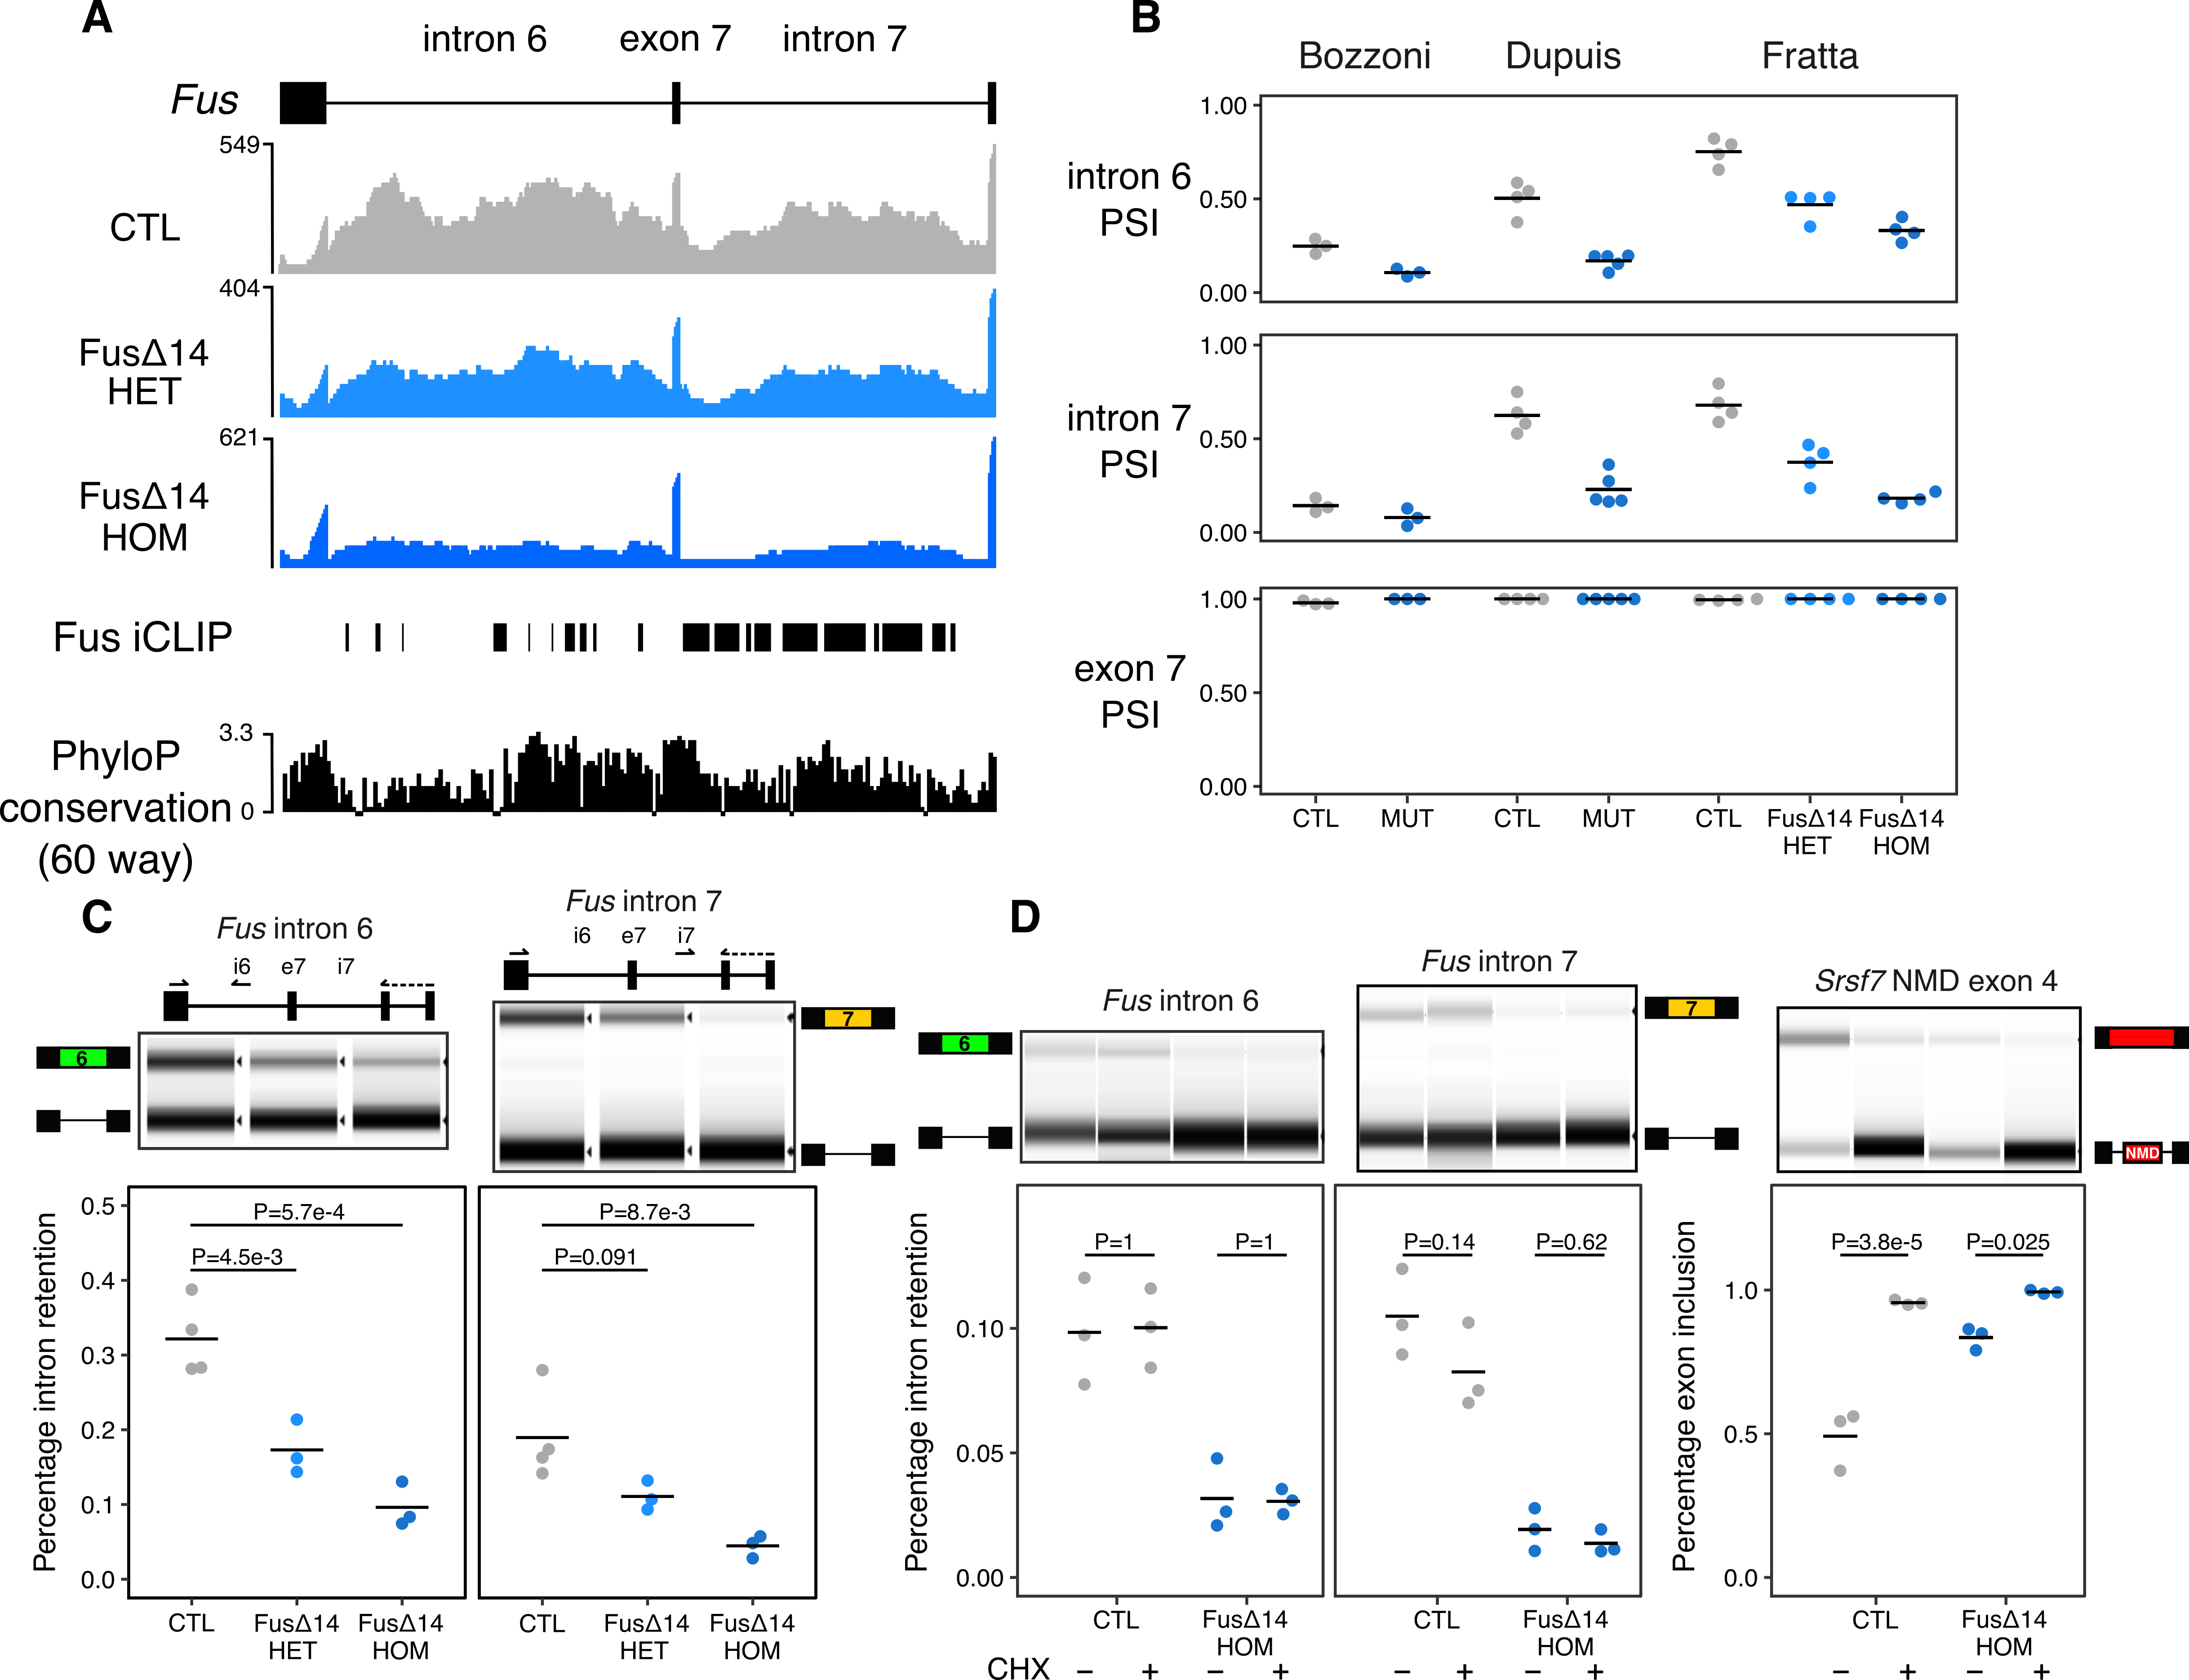
\includegraphics[width=\textwidth]{Figures/06_fus_meta/Fus_autoregulation.png}
	\caption[FUS intron retention is an NMD-insensitive autoregulation mechanism]{
		\textbf{Fus intron retention is an NMD-insensitive autoregulation mechanism.}
	\textbf{(A)} FUS introns 6 and 7 are highly conserved and have multiple FUS iCLIP binding peaks. 
	Retention of introns 6 and 7 decreases with increasing dose of FUS $\Delta$14. 
	RNA-seq coverage for wildtype, FUS $\Delta$14 heterozygous and FUS $\Delta$14 homozygous samples are accompanied by FUS iCLIP \citep{Rogelj2012} and PhyloP conservation (60 way) tracks.
	\textbf{(B)} Percentage spliced in (PSI) values of intron 6, intron 7 and exon 7 in the three datasets, including the FUS $\Delta$14 heterozygotes.
	\textbf{(C)} RT-PCR validation of the reduction in intron 6 and 7 inclusion with increasing dose of FUS $\Delta$14 mutation. 
	Left panel - FUS intron 6 (ANOVA genotype \textit{P}=5.1e-4; t-test CTL vs HET \textit{P}=4.5e-3; CTL vs HOM \textit{P}=5.7e-4)
	Right panel - FUS intron 7 (ANOVA genotype \textit{P}=8.5e-3; t-test CTL vs HET \textit{P}=0.091, CTL vs HOM \textit{P}=8.7e-3)
	\textbf{(D)}	Translation blocked with cycloheximide (CHX) to observe whether the intron retention transcript is sensitive to nonsense-mediated decay. 
	Left panel: FUS intron 6 retention is not altered with CHX treatment. ANOVA treatment \textit{P}=0.96; genotype \textit{P}=1.9e-5; t-test CTL untreated vs CTL treated \textit{P}=1; HOM untreated vs HOM treated \textit{P}=1.
	Middle panel: FUS intron 7 retention is unchanged by CHX treatment. ANOVA treatment \textit{P}=0.10; genotype \textit{P}=3.7e-6; t-test CTL untreated vs CTL treated \textit{P}=0.14; HOM untreated vs HOM treated \textit{P}=0.62.
	Right panel - \textit{Srsf7} exon 4, a known NMD target, is increased by CHX treatment. ANOVA treatment \textit{P}=5.3e-4; genotype \textit{P}=0.011; t-test CTL untreated vs CTL treated \textit{P}=3.8e-5; HOM untreated vs HOM treated \textit{P}=0.025.
	All reported \textit{P}-values are corrected for multiple testing.
	}	
	\label{fig:fus_autoregulation}
\end{figure}


% explain FUS autoregulation
The joint splicing analyses found 5 intron retention events in FUS itself.
3 of these are knockout-specific and probably result from increased intronic reads in the partial Bozzoni knockout samples. 
However, The 2 remaining introns (introns 6 and 7) were also found in the FUS NLS mutants.
These introns overlap with a large number of FUS iCLIP binding peaks and could be the site of regulation of the \textit{Fus} transcript by the FUS protein.
Many RNA-binding proteins have the ability to bind their own RNA to control the level of their own translation, a phenomenon known as autoregulation \citep{Rosenfeld2002,Jangi2014a}.
When protein levels are high, protein-RNA binding shifts splicing towards the production of an non-coding isoform.
This is commonly through exposing transcripts to nonsense-mediated decay (NMD) \citep{McGlincy2008-wh}, by including an exon containing a premature stop codon as in HNRNP L and NOVA \citep{Rossbach2009,Dredge2005}, skipping a frame-preserving exon as in PTBP1 \citep{Wollerton2004}, or splicing within the 3\'\ UTR as in TDP-43 \citep{Ayala2011}. 

RNA-protein interaction experiments have revealed a large cluster of FUS binding across introns 6 and 7 of the FUS gene \citep{Lagier-Tourenne2012}, both of which show very high sequence conservation between species.
This region was previously suggested to be the locus of autoregulation due to both an annotated cassette exon event in exon 7 and an a early polyadenylation transcript being present in transcript annotation databases (Ensembl, Refseq).
Skipping of exon 7 is predicted to cause a frameshift which should trigger NMD. 
Zhou and colleagues first investigated the mechanism of FUS autoregulation by inhibiting NMD and looking at changes in splicing of exon 7 \citep{Zhou2013}.
The exon-skipping transcript increased when FUS was overexpressed and decreased when FUS was knocked down, suggesting this splicing event to be the autoregulatory mechanism.
However this mechanism does not explain the high sequence conservation of the diffuse FUS binding pattern across introns 6 and 7 (Fig. \ref{fig:fus_autoregulation}A).
When examining RNA-sequencing coverage of the FUS gene in the Fratta, Bozzoni and Dupuis datasets, I could not observe any changes in the inclusion of exon 7 in any sample.
However I could observe a strong retention of both introns 6 and 7 that decreased in the presence of FUS NLS mutations. 
This phenomenon can be seen in all three datasets (Fig. \ref{fig:fus_autoregulation}B), despite the baseline level of retention in wildtype cells being highly variable. 
We generated RNA sequencing data from mice heterozygous for the $\Delta$14 NLS mutation. 
Comparing wildtypes, heterozygous and homozgous FUS $\Delta$14 samples showed that retention of introns 6 and 7 decreased with dose of the mutation (Fig. \ref{fig:fus_autoregulation}A/B) .

We designed an RT-PCR assay to validate the intron retention changes with a three primer method that could amplify a spliced transcript spanning \textit{Fus} exons 6-7-8-9 with a second band for either exon 6-intron 6 or intron 7-exon8. 
Intron retention decreased in a mutation dose-dependent manner (intron 6 \textit{P}=5.7e-4; intron 7 \textit{P}=8.7e-4; ANOVA; Fig. \ref{fig:fus_autoregulation}C).
We failed to detect a band corresponding to the skipping of exon 7 in any sample. 

Retaining two introns would be expected to cause NMD through premature stop codons, which are abundant in both intron 6 and 7. 
This has been proposed as the main degradation pathway for intron retention transcripts \citep{Wong2013}, although the  nuclear retention and elimination (NRE) has also been implicated \citep{Yap2013}. 
To test whether the intron retention FUS transcript undergoes NMD we reran the RT-PCR experiments after inhibiting translation in mouse fibroblasts with cycloheximide for 6 hours.
This should cause NMD to be inhibited as NMD requires transcripts to be bound to the ribosomes.
No effect on intron retention by cycloheximide treatment was seen in either wildtype or FUS $\Delta$14 homozygous fibroblasts (Fig. \ref{fig:fus_autoregulation}D).
As a positive control I used the inclusion of a known NMD-sensitive exon in \textit{Srsf7} \citep{Edwards2016}, which increased in both genotypes. 

These experiments suggest that depleting nuclear FUS protein downregulates the production of an intron retention transcript insensitive to nonsense-mediated decay. 




%Yap2013 - intron retention in neurons of terminal 3\' introns detains neuronal-specific transcripts in the nucleus which are eventually degraded not by NMD but by RNA surveillance proteins. and then switch to splicing out and cytoplasmic transport when Ptbp1 levels change

% negative feedback mechanism
% protein homeostasis
% protein binds own mRNA
% changes in protein levels alters the splicing of the mRNA from a productive isoform to an isoform susceptible to nonsense-mediated decay, by skipping a frame-conserving exon, or by introducing a poison exon.
% iCLIP experiments have revealed that Fus binds a large section of its own mRNA spanning ~ 3500bp comprising intron 6, exon 7 and intron 7. 
% Both introns show very high conservation between species, suggesting an important regulatory role for the introns.
% \cite{Zhou2013} and colleagues used RT-PCR to show that changes in FUS protein levels alters the inclusion of exon 7 and the exon 7-skipped transcript is sensitive to nonsense-mediated decay.
% Inspecting the RNA-seq traces from our data as well as Dupuis and Bozzoni, we see no evidence for any change in exon 7 inclusion in the presence of NLS mutated FUS.
% Instead we see a clear reduction in the retention of introns 6 and 7.
% Using RNA-seq data from the heterozygous FUS $\Delta$14 mice it is clear that the reduction in intron retention is dependent on the mutation dosage.

% To validate the intron retention changes I developed an RT-PCR assay with primers targeting exon 6 and exons 8/9 to selectively amplify spliced FUS mRNA and an additional third primer targetting either intron 6 or intron 7. This three primer PCR amplifies bands corresponding to intron 6 and 7 retention and splicing. Our primers did not amplify a band corresponding to exon 7 skipping. 
% With increasing dosage of the FUS $\Delta$14 mutation the proportion of intron retention reduces for both intron 6 and intron 7 (Figure \ref{fig:fus_autoregulation}C).

\section{Discussion}

% Reiterate what I've done and seen
This study is the largest transcriptome-wide assessment of FUS function to date.
By combining three separate datasets of FUS knockdown and NLS mutation I have been able to discover a large repertoire of differentially expressed genes and differential splicing events that have not previously been reported.
Comparison of the two conditions demonstrates that NLS mutations predominantly act to reduce nuclear FUS, as the majority of expression and splicing changes overlap and change in the same direction.
This leaves only a small number of NLS mutation-specific gene expression changes and almost no mutation-specific splicing changes other than in FUS itself. 
By studying the mutation-specific splicing changes in FUS I have discovered a novel intron retention transcript that could explain the mechanism by which FUS regulates its own translation.

The joint modelling approach has allowed me to combine three different RNA sequencing datasets to produce a consensus set of RNA phenotypes.
Due to the stochastic nature of transcription and splicing combined with the small sample sizes employed, these datasets are inherently variable.
By combining repeated observations  under the same genetic conditions we can better discover true FUS-associated changes.
While joint modelling increases detection power, it rewards conformity between experiments and I cannot discount the possibility that each dataset has its own cell-type or mutation-specific effects confounded with the dataset itself.
It is arguable that these dataset-specific changes are more likely than not to be biologically irrelevant such as transgene insertion artefacts. 
In addition, with increased power I can now detect changes in expression and splicing at very small effect sizes. 
While this provides more information, the biological relevance of these small changes is harder to investigate.
These changes are less likely to be a direct result of FUS RNA or protein interaction and may emerge through multiple downstream effectors or pathways.
%As a disease-associated protein, FUS has been intensely studied and the number of putative roles it has within the cell is large.  

Employing a relaxed significance threshold demonstrated that the majority of changes are shared between  FUS knockout and NLS mutation.
The direction of change was identical for 99\% of overlapping genes with a clear bias towards stronger changes in the knockout (Fig. \ref{fig:fus_expression_multipanel}B). 
This is unsurprising, as NLS mutations do not completely abolish FUS nuclear import \citep{Scekic-zahirovic2016, Devoy2017}.
% neuronal gene loss
There is a widespread downregulation of neuronal and synaptic genes in FUS nuclear depletion. 
This could be due to defects in RNA transport as FUS has been found in RNA transport granules \citep{Kanai2004, Fujii2005}.
% splicing factor upregulation
Conversely, RNA binding genes were upregulated in both conditions. 
FUS is known to interact on a protein-protein level with multiple splicing factors \citep{Yang1998,Meissner2003, Groen2013} and particularly members of the U1 snRNP complex \citep{Sun2015a, Yu2015a}. 
CLIP experiments show that FUS binds a number of these factors at the RNA level \citep{Nakaya2013}.
Therefore FUS is part of a complex network of RNA and protein interactions with multiple splicing factors. 
However, why FUS loss acts to upregulate these factors is yet to be discovered.
% Xlr genes
I managed to replicate the finding of upregulation of the X-linked lymphocyte receptor (\textit{Xlr}) cluster of genes, first seen in adult FUS knockout mice \citep{Kino2015}, suggesting that FUS loss causes chronic dysregulation of these genes. 
As Xlr gene overexpression can alter dendritic spine growth and are regulated by the Cux1/2 transcription factors \citep{Cubelos2010}, the mechanism of how FUS loss leads to their upregulation is intriguing. 
No FUS iCLIP clusters were observed overlapping any Xlr gene, discounting direct post-transcriptional regulation.
As these genes appear to be mouse-specific they are not directly relevant to disease but could provide a useful model for the effect of FUS on transcription.

% Splicing
Overlapping the joint splicing models demonstrated that almost all splicing changes attributed to NLS mutations could also be observed in FUS knockouts.
I did not observe a convincing set of mutation-specific splicing changes which is unsurprising as splicing is a nuclear function. 
The overlap between knockdown and expression has been seen in cells where overexpression of NLS mutant FUS cannot rescue splicing changes in FUS knockdown cells \citep{Sun2015a}.
Due to the multiplicity of FUS interactions between multiple splicing factors, disturbance of any or all of these factors could be confounding the splicing changes. 
For example, the splicing profiles of FUS NLS mutations overlap those from knockdowns of known interactor SMN \citep{Mirra2017}.
I observed approximately double the number of 5\' splice site changes than 3\' splice site changes. 
This could be due to the shorter length of the consensus 5\' splice site sequence compared to the 3\' making cryptic splice sites more likely by chance, but it may hint at a consequence of the interaction between FUS and the U1 snRNP.
Although the interaction between FUS and the U1 snRNP has been well studied \citep{Nakaya2013,Yu2015a,Yu2015b}, my analysis has uncovered a large array of splicing events to study the role of FUS in splicing.

The dominance of retained introns and complex events (where multiple splice sites are altered simultaneously) points to a more nuanced picture of splicing changes than has previously been investigated in RNA-binding protein biology.
I concede however that the large number of complex events seen in the joint splicing models is probably a result of the juction-centric method I used, as well as analysing all the data jointly. 
An isoform-centric approach where reads are assigned to specific transcripts \citep{Trapnell2010,Bray2016} perhaps would more sensitively tease out the different changes that are happening in complex introns.

% SPLICING AND TRANSCRIPTION - REWRITE

Nevertheless, complex events as well as intron retention events are enriched in FUS iCLIP binding and are more likely to affect splicing factors than the cassette exons I observed. 
This suggests a more subtle role for FUS in splicing than simply altering alternate cassette exons which have been the focus on previous studies on FUS and splicing \citep{Rogelj2012,Lagier-Tourenne2012,Ishigaki2012,Honda2014,Scekic-zahirovic2016}.
FUS can bind the C-terminus of RNA polymerase II \citep{Schwartz2012} and a study on the role of FUS in alternate polyadenylation suggested that FUS binding to pre-mRNA can stall RNA polymerase II \citep{Masuda2015}. 
Transcriptional speed is known to affect splicing as pausing transcription can allow more time for splicing factors to bind weaker affinity sequences \citep{Kornblihtt2004a}. 
Splicing events altered when transcriptional elongation is reduced are enriched for RNA binding genes \citep{Ip2011}. 
This suggests that the intron retention events seen in FUS knockout and mutation, including \textit{Fus} itself may arise from FUS stalling RNA polymerase II.

The high sequence conservation seen in retained introns suggests a regulatory role for these splicing events, despite the unexpectedly low overlap between splicing changes and differentially expressed genes.
One example of this is the U1 splicing factor \textit{Snrnp70}, whose highly conserved intron retention transcript has previously been shown to increase in FUS knockdown, which should lead to increased degradation of \textit{Snrnp70} mRNA through nonsense-mediated decay \citep{Nakaya2013}. 
Two overlapping splicing events are found in \textit{Snrnp70} that suggest the NMD-sensitive conserved intron section is more retained in FUS knockout. 
I observed upregulation of \textit{Snrnp70} in the FUS knockouts, although this gene-level metric may confound the change in isoforms suggested by the splicing analysis. 
The other FET family members \textit{Taf15} and \textit{Ewsr1} are both upregulated and both contain conserved intron retention events that are more frequently skipped in FUS depletion.
For \textit{Taf15}, its upregulation when FUS is depleted is probably a redundancy mechanism due to the shared RNA motifs and target genes of the two proteins \citep{Ibrahim2013,Kapeli2016}. 
The splicing changes I identify in both \textit{Taf15} and \textit{Ewsr1} suggest a mechanism for how their expression is increased when  nuclear FUS is depleted.
A previous study did not find the mRNA stability of \textit{Taf15} to be changed in FUS knockdown \citep{Colombrita2012} but this requires re-evaluation in light of the new data.

By studying our RNA-seq data in all three NLS mutant datasets I observed a novel intron retention isoform whose retention inversely correlates with the dose of NLS mutation. 
As the change can also be observed in mice heterozygous for the FUS knockout allele it is unlikely to be due to the mutant NLS itself (data not shown).
Although cassette exon skipping of exon 7 was previously suggested to be the splicing event of FUS autoregulation \citep{Zhou2013}, neither our RNA-seq or RT-PCR observed exon 7 skipping in the presence of NLS mutation.
This could simply be due to exon 7 skipping being present but at much lower level than intron retention changes. 
Zhou and colleagues could not have detected intron retention changes as the length of the retention transcript exceeds the maximum amplicon length for PCR. 
Our three-primer approach robustly demonstrated the changes in retention occur in both introns 6 and 7 but they cannot conclusively prove simultaneous retention of both introns. 
% Premature polyadenyaltion?
This would require a long-read sequencing technique. 
The NMD inhibition experiments suggest that the FUS intron retention transcript is insensitive to nonsense-mediated decay. 
Although, cycloheximide inhibits translation in order to inhibit NMD and off-target target effects cannot be excluded. 
To elucidate this as the mechanism of FUS regulation, further experiments are needed to validate this in human cells.
One possible mechanism is that the transcript is instead detained in the nucleus.
This is a regulatory pathway proposed for intron retention transcripts to prevent translation \citep{Boutz2015}.
A analogous mechanism for autoregulation has been proposed for TDP-43, where the binding of TDP-43 protein to \textit{Tardbp} mRNA shifts polyadenylation to create a long 3\'\ UTR transcript which is detained in the nucleus and degraded by the exosome. The long transcript can also be spliced to form NMD-sensitive isoforms which can be exported to the cytoplasm and then degraded \citep{Ayala2011,Koyama2016}. It is unclear why the system would require two separate degradation pathways. 
In the light of this, the discovery of the FUS intron retention transcript could be a complementary mechanism to the one set out by Zhou and colleagues.
This would then answer the outstanding question of the high evolutionary conservation of both introns and the length of FUS binding throughout.

% ALS biology implications
This study combines multiple RNA sequencing experiments to better understand and catalogue changes in gene expression and RNA splicing in response to FUS nuclear depletion.
My analysis suggests that these changes are shared due to the extreme overlap and concordance of direction of gene expression and splicing.
It does not conclusively link any of these alterations to motor neuron toxicity and degeneration, which is only seen in NLS mutant embryos and not in FUS knockouts \citep{Scekic-zahirovic2016}.
It is unclear whether toxicity can be attributed to the 186 mutation-specific genes due to the sharing of gene ontology categories with the overlapping set (RNA processing and synaptic genes). 

The discovery of a novel mechanism for FUS autoregulation is valuable for understanding the role of FUS in disease.
Autoregulation acts to maintain protein homeostasis but FUS NLS mutations interfere with this.
When FUS nuclear import is abolished by mutations, there is no way for FUS protein to regulate  its own translation, leading to ever-more cytoplasmic FUS.
High concentrations of cytoplasmic FUS increase the likelihood for aggregation which NLS mutant FUS is more prone to do \citep{Bosco2010}. 
This increased propensity may be due to the recent finding that NLS acts to solubilise FUS aggregates through binding to Transportin \citep{Guo2018,Yoshizawa2018,Hofweber2018}.
In FUS ALS, patients only have a single copy of NLS mutant FUS. 
Selectively removing the mutant copy, at either a DNA or RNA level, should all but prevent cytoplasmic mislocalisation while maintaining nuclear FUS levels due to the compensatory nature of autoregulation. 
Indeed, mice heterozygous for a FUS knockout allele have FUS mRNA and protein levels at 75\% of wildtypes and exhibit no motor neuron degeneration \citep{Scekic-Zahirovic2017}. 
This could feasibly be increased to 100\% by modulating FUS autoregulation by promoting the splicing of introns 6 and 7. 
This work expands our understanding of the complex role of FUS in gene expression and splicing and uncovers a new model for FUS autoregulation. 
I hope this will be useful to the disease field in designing targeted therapies for FUS ALS.

% Largest transcriptome-wide study of FUS function to date
% Discovered a large number of differentially expressed genes and differential splicing events
% Discovered a novel mechanism for FUS autoregulation via intron retention.

%% Joint modelling

% Importance of replication
% RNA is inherently noisy
% Joint modelling provides clarity

% Joint models boost power but they reward conformity between datasets
% There may be important biological differences, such as subtle cell type or developmental differences that account for different genes and splicing events ocurring in different datasets

% Between sample variance clearly important to detecting RNA changes
% Unexplained why such a difference
% Any evidence of a polyA / total RNA effect on variance?

%% Gene expression
% We find the largest set of gene expression changes associated with FUS depletion.
% Knockout and NLS mutation have a strong overlap that is biased towards the knockout
% This makes biological sense as NLS mutations don't completely ablate nuclear import
% 99% of genes go in the same direction but 7 genes are upregulated in the FUS mutant
% P values are unconvincing but 3/7 have FUS binding so could be real, worth following up



% full-blown nuclear FUS depletion would only occur at disease endpoint
% adult loss of FUS is not toxic to motorneurons but would cause many changes in splicing factor biology
%  single copy FUS NLS mutations are still highly toxic


% We see more 5\' changes than 3\', implicating U1 impairment
% How many of the intron retention changes are due to U1-sensitivity? Are retained introns more sensitive to spliceosomal changes?

% No convincing splicing changes found to be mutation specific
% not surprising as this should be a nuclear function of FUS

% Retained introns are enriched for RNA binding function and FUS binding
% Previously seen for Snrnp70 - U1 factor
% This makes sense as FUS can interact with the whole U1 snRNP
% We have extended this to a larger group of proteins

% Cassette exons are not, this is surprising
% Boris found enrichment of FUS peaks within 200bp  of cassette exons whereas we took the entire intron and found no enrichment. Targeted appraoch is probably better.
% FUS's role in alternative exon splicing perhaps overstated

% Retained introns in RNA binding proteins suggests NMD mechanisms
% FUS is part of network of splicing factors that all cross-regulate
% Not surprising that mislocalisation of FUS triggers changes in other factors
% Taf15 and Ewrs1 obvious candidates to replace FUS, redundancy in system

% Complex events inherently difficult to interpret
% Here an isoform-level approach would be more effective
% Caveat is when one is interested in novel isoforms, as are important in TDP biology (cite my papers)

% theme - FUS alters splicing and gene expression of genes coding for proteins that FUS is known to interact with - U1 snRNP, hnRNPs, FET proteins, YBX1 \citep{Groen2013}.


%% Autoregulation 
% We have identified a new mechanism for FUS autoregulation
% Is it prematurely polyadenylated?
% RT-PCR primers are targeting isoform with exon 9 included which should be downstream of any premature polyadenylation site.

% why don't we see the Zhou exon 7?
%% No evidence from RNA-seq so skipping transcript may just be very lowly expressed.
% They wouldn't pick up intron retention due to being too long to amplify by RT-PCR.
% Our data suggests that FUS intron retention changes FUS protein levels through a change in mRNA localisation rather than nonsense-mediated decay
% Cite detained introns paper, Pimental paper.


% Implications for ALS biology

% FUS gain of function may take a long time to appear, all data is embryonic
% All models are homozygous, does not reflect ALS patient biology


% Differential expresion differences 
%This is probably due to a larger sample size and the fact that their data is polyA+ enriched, which will potentially reduce the between-sample variation allowing for more precise measures of between-condition differences. 
%It is also possible that how they prepared the tissues and extracted the RNA resulted in less variability between samples than the Bozzoni and Fratta datasets.
%\chapter{Discussion}

%appreciate the limitations of the methods employed and the results obtained by yourself and others
%understand how the broad conclusions of your thesis support, add to or conflict with previous work

% Sum up findings of four chapters

In my thesis I have analysed multiple RNA-seq datasets to uncover new insights into TDP-43 and FUS.
This work has explored the physiological roles of the two proteins in RNA regulation through loss-of-function experiments.
Furthermore, by using mutant mice as models of disease, I have uncovered mechanisms by which disease-associated mutations can impart a gain-of-function. 
This comparison between loss- and gain- is crucial for understanding the onset and course of ALS/FTD.

In chapter 3 I developed software to discover and classify the full extent of cryptic splicing repression by TDP-43 and applied it to multiple mouse and human datasets.
I demonstrated that this repression is due to a combination of UG motifs and strong splice sites found within poorly conserved introns.
In normal conditions TDP-43 will compete with the spliceosome to prevent aberrant recognition of these sequences as exons.
Upon TDP-43 depletion these exons are included which leads to transcript instability, probably through nonsense-mediated decay (NMD).
These changes can be seen at the level of gene expression.
This mechanism was not seen in FUS knockdown, suggesting a divergence in function for the two proteins.
Later work has shown that cryptic exon repression is seen in a range of RNA-binding proteins, including the ALS associated MATRIN3, SFPQ and TIA1.

In chapter 4 I analysed data from a novel FUS mutant mouse which modelled aggressively early onset FUS ALS. 
By looking at two tissues and two timepoints I identified a specific transcriptomic signature seen only in late-stage mouse spinal cord.
This was dominated by changes in mitochondrial and ribosomal genes.
Splicing changes at this tissue and time point were restricted to FUS itself and a small number of other genes including the myelin protein \textit{Mbp} and the FUS-interacting RNA-binding protein \textit{Ewsr1}.

In chapter 5 I compared two TDP-43 mutant mice, where one mutation caused a loss of splicing function due to the mutation affecting an RNA-recognition motif. 
The second mouse line had a mutation within a hotspot for ALS mutations, the low complexity domain.
I demonstrated that this mutation imparts a gain of splicing function, where instead of aberrant exon inclusion as seen in TDP-43 loss, there were a set of aberrant exon skipping events.
I christened these events "skiptic exons" and showed that these affect constitutive exons and their skipping would more often than not lead to frame shifting and transcript degradation through nonsense-mediated decay. 
Some of these skiptic exons could be identified in TDP-43 mutant human patients.
I posit that the gain of splicing function could arise from a change in TDP-43 autoregulation.

In chapter 6 I compared three independent experiments where FUS was either knocked out or mutated to remove its nuclear localisation signal (NLS) in mouse neuronal tissues.
My joint analyses demonstrated significant overlap between the two FUS conditions in both gene expression and splicing, suggesting that FUS NLS mutations primarily deplete FUS from the nucleus.
Looking in detail at the FUS locus itself, I identified a novel mechanism by which FUS could regulate its own translation through intron retention. 
This autoregulation mechanism may be complementary to one previously reported exon skipping \citep{Zhou2013}.

All together, my results suggest specific consequences for loss of TDP-43 or FUS and gains of function in the cytoplasm, as seen in ALS/FTD.

\section{Issues arising from my work}

\subsection{Loss and gain of splicing function in TDP-43 and FUS}

% TDP loss leads to de-repression of cryptic exons
% these exons are not conserved between human and mouse - presumably due to lack of conservation of introns
% many alternate exons regulated by TDP are not conserved either or differ greatly in their change in response to TDP between human and mouse
% even within the same species they do not completely overlap between datasets
% each dataset has unique sets of exons
% This was seen in another study comparing TDP-43 deletion in mouse neurons, muscle cells and stem cells \citep{Jeong2017}.
% Each cell type will have a different set of RBPs expressed and binding to the same introns.
% the two human K562 cell datasets from ENCODE do not fully overlap despite being the same cell type
% some of this is probably technical due to polyA+ vs Total RNA
% but even the smaller list of total RNA cryptic exons are not merely a subset of the larger polyA + exons

Since I began studying TDP-43 and cryptic exons, many more RNA-binding proteins have been found to have a role in cryptic exon repression including PTBP1/2, RBM17, hNRNP L and MATR3 \citep{	Ling2016,Tan2016,McClory2018,Attig2018}. 
My own assessment of ENCODE knockdown data on a large number of RBPs showed that cryptic exon repression is a common feature seen in nearly all knockdowns with the exception of FUS (see chapter 3). 
% how important is loss of function to disease?

% multiple mouse models have shown that neurodegeneration can occur both without loss of TDP or FUS splicing function nor cytoplasmic aggregates.
% Mice are not humans




\subsection{RNA-seq allows replication }

% Replication crisis - why most published results are probably false

% replication of the same phenonmenon in the same protein or model

% also, is a particular phenomenon common or specific to a particular protein?

% Both TDP-43 and FUS are linked to an every expanding list of roles within the cell, how many of these have been replicated?

% Open platform of RNA-seq, combined with data sharing and code sharing allows rapid replication to be done as standard.

% Caveats - particular phenomena may only be seen under certain experimental conditions or in particular cell types
% Example - circular RNA only seen with confidence when linear RNA are digested


\section{Future directions for the work}

\subsection{Translating work into human patients}

It is regretful that throughout my PhD I have not had the opportunity to explore more human RNA-seq samples and particularly those from human patients.
The reason for this is partly due to scarcity of tissue but also the technical hurdles in analysis.
Unlike laboratory strains of mice, humans and highly heterogenous in both their genetics and the environmental exposures.
Even patients with identical mutations in a disease-associated gene could  expected to have many distinct modifying mutations as well as completely different life experiences.
Therefore any study on transcriptomics in humans would require much larger sample sizes to account for the increased variability in measurements of gene expression and splicing.
ALS/FTD patients would be expected to be particularly heterogenous due to the above genetic differences as well as variability in disease course and extent of pathology at death.

There are also technical considerations in sequencing post-mortem brains.
Both ALS/FTD patients and non-neurological control donor brains will often come from human patients who were kept on artificial respiration before death. 
This is known to affect RNA quality in post-mortem tissue due to changes in tissue pH.
This is the reason for most post-mortem tissue RNA-seq samples are prepared using total RNA libraries which may then dilute the amount of reads that will align to protein-coding genes of interest.

There are now large consortia established to collect and sequence large numbers of patient brains. 
As part of my post-doctoral studies I am looking forward to working with these consortia.

An alternative route for studying ALS/FTD in human brains is to grow patient neurons from induced pluripotent stem cells (iPSCs).
%These can be created from skin samples from patients and through a lengthy process, mature neurons can be created.

 neuronal organoids can be created. 
These can contain a variety of neuronal and glial cell types and replicate some basic topology of a human brain, with cells distributing to layers.


\subsection{Diving deeper into RNA regulation}

% bulk cell sequencing - need single cells
This work was all done with bulk cell short read RNA-seq. 
There are limitations to this approach that are both biological and technical.
Bulk RNA sequencing samples RNA from all cells in a population. 
This limits the observations that can be made to changes in expression and splicing that can be seen across a wide range of cells with low variability between cell types.
A rapidly developing solution to this is single-cell RNA sequencing, where individual cells are first separated from a tissue and sequencing libraries prepared using microfluidic technology.
Studies are now emerging of 10s of 1000s of individual cells being profiled. 
This has allowed for example an entire mouse brain to be classified into different cell types. %ref
The technology for this is still in its infancy and there is a problem with sequencing throughput to get enough reads per sample.
This will be important to overcome for analysing splicing changes due to the need for splice junction reads.
It would be very exciting if this technology could be applied to ALS/FTD patient brains. 

% need specific populations of RNA
Bulk sequencing also removes the distinction of RNA localisation within different cellular compartments. %distinction wrong word
For example, both FUS and TDP-43 bind transcripts in the cytoplasm and have some role in axonal transport. %ref
Fractionating RNA into nuclear or cytoplasmic would give information about nuclear retention of particular transcript, as I hypothesise for the FUS intron retention transcript identified in chapter 6.
Growing neurons in compartments as in \citep{Taliaferro2016} would allow specific populations of transcripts to be sequenced.
Alternatively, sequencing the nascently transcribed RNA would allow observation of unstable transcripts.
The nagging question from chapter 3 is that if I predict most cryptic exons to be degraded by NMD, why do I see any at all?
Silent splicing events were proposed in RBFOX proteins \citep{Jangi2014} to explain gene expression changes in RBFOX2-bound transripts without splicing changes.
If we were to sequence nascently transcribed RNA, perhaps with 4 thio-uridine, I could identify unstable transcripts that rapidly degrade upon export to the cytoplasm.
This may demonstrate cryptic splicing repression by TDP-43 to be much more widespread and why certain cryptic exon transcripts appear to evade NMD.



% problem with bulk sequencing
% lose cell-type specific information
%% single-cell RNA seq can do this
%% in disease brain one could select just cells with TDP or FUS pathology for analysis
% lose RNA localisation information
% some isoforms are preferentially transported - see Taliaferro
% Cytoplasmic NLS mutant FUS will play a role in transport - would need to fractionate

%Bulk cell or whole tissue sequencing means a loss of resolution
%RNA extracted from entire sections of tissue or populations of cells
% problem with short read sequencing
% cannot easily resolve complex transcripts
% evidence that some splicing events are co-regulated from Tilgner et al, need long reads to see this
% intron retention would be much simpler to detect
% still issues with throughput and error rate
Short reads






\section{Final thoughts}


% TDP but not FUS represses cryptic exons
% However cryptic exon repression can be seen in many RNA-binding proteins
% Repression of intronic sequences will be achieved by multiple proteins simultaneously
% "Crypic exons" that we see are just the tip of an iceberg, those sites where a single protein does most of the work
% Would explain low overlap between different knockouts in the same species
% Follow up paper showed lack of overlap between different mouse tissues

% TDP LCD mutations cause a gain of splicing function
% Inverse to cryptic exons, this is a role in maintaining canonical splicing that is being altered somehow by the mutation
% Suggests a spectrum between surveillance and maintenance functions
% Canonical splicing must be maintained and aberrant splicing must be repressed.
% TDP has roles in both
% It would be interesting to look through a range of RBPs and assess their skiptic and cryptic contributions - do they fit on a spectrum?
% Might expect proteins more deeply involved with the spliceosome to be more involved in supporting canonical exons than repressing
% Although one could also expect both functions depending on the position of binding, as are seen for alternate exons.

% FUS diverges from TDP, despite having shared roles in long intron genes, RNA transport and stress granules
% FUS does not repress cryptic exons, this could be due to weaker motif
% FUS KO and NLS mutations overlap, essentially both are loss of FUS function
% Splicing changes show few cassette exons and these are not enriched in iCLIP peaks.
% Excess of intron retention and complex events potentially an artefact of total RNA libraries, although the Dupuis dataset is polyA+ and contributes somewhat to splicing although less than the others.

% All the high quality mouse TDP data is polyA+ enriched so cannot make a fair comparison with the FUS knockout data.
% This loss of function is not seen in studying the delta 14 mice, as very few splicing events are seen.
% Gene expression profiles are completely different between embryonic HOM D14 and 12 month HET D14.
% The former shows neuronal and RNA binding terms, probably due to acute FUS loss
% Mitochondrial and ribosomal changes seen in 12 month D14 could be due to gain of function
% Other observations of FUS granules in the paper right?




% What does this mean for studying TDP and FUS?
% Two proteins have different functions
% They diverge on crypic exons



% What does this mean for ALS/FTD?
% Loss of RBP function is only one facet and it will be important to untangle these effects from a gain of function. The LCDmut shows that  without aggregation there is a specific effect on splicing, which can also be seen in human ALS patients


% What does this mean for RNA biology?



% What kind of work will follow this?










%\chapter{Next Steps for my PhD}
%
%My work so far has been on two very different projects centering around RNA regulation in models of ALS/FTD. The cryptic splicing project in TDP-43 was based on public data, which allowed for rapid progress and the ability to replicate my conclusions across multiple experiments. However, brute force knockdown of TDP-43 is a very crude model of disease and the project suffered from the low quality of RNA-seq data and the inability to validate the mechanism with a wet lab collaborator. The FUS $\Delta$14 mouse project however offers up a humanised mouse model where disease-like changes occur progressively. There is much appetite from Anny Devoy and from the lab of Pietro Fratta to continue investigations into the mechanism of the mutation's effect on RNA regulation.\\ 
%
%Over the remainder of my PhD I plan to upgrade the RNA-seq pipeline to use state-of-the-art splicing analysis software. I will then apply this pipeline to better understand the changes in splicing that occur in the FUS $\Delta$14 mouse, as well as in new data being generated on the mutation's impact on mRNA transport and translation. I will also apply the splicing pipeline to two opposing \textit{TARDBP} mutant mice and compare the results with existing TDP-43 knockdown data. To continue the cryptic splicing project I will screen the large ENCODE cohort of RNA-binding proteins for cryptic exon repression and then look for evidence of cryptic splicing in ALS/FTD patient brains. 
%	
%
%\section{Developing a full-featured splicing analysis pipeline}
%Since I started work on \textit{CryptEx} in October 2015 there have several major advancements in algorithms to analyse differential splicing from RNA-seq data. This has been enabled by improvement in the quality of RNA-seq data. \textit{CryptEx} and the underlying \textit{DEXSeq} approach were designed to work on all qualities of data going back to low depth, short read datasets generated in 2010. So while it has been useful for the TDP-43 project I believe I should make use of the state-of-the-art tools now available. Dr Kitty Lo and I have installed and assessed the latest advances in RNA-seq analysis algorithms. We can group software packages into one of four categories based on what they consider to be the fundamental unit of differential splicing. All of these modern algorithms require paired end data with high coverage and long reads to maximise the information available.
%
%\subsection{Transcript quantifiers}
%These compare abundances at the transcript level and rely on a curated list of known transcripts. Sequencing reads are then probabilistally assigned to a each transcript. This can be done extremely quickly in the case of pseudoaligners like \textit{Kallisto} \citep{Bray2015}. Transcript assembly algorithms like \textit{Stringtie} \citep{Pertea2015} can even assemble reads into novel transcripts. These algorithms require long reads for enough splicing information and very dependent on the list of transcripts they are given. Some genes can generate hundreds of very similar transcript isoforms or overlap with other genes and so these methods will struggle to accurately assign reads to them.
%
%\subsection{Exon quantifiers}
%These algorithms are typified by the \textit{DEXSeq} approach \citep{Anders2012}, where the transcripts are flattened to create a set of unique exon "bins".  As the bins themselves may not actually be an exon it makes the results difficult to interpret, although this has been lessened in a new software package called \textit{JunctionSeq} \citep{Hartley2015}, which also quantifies splice junctions and can pick up novel splice junctions. As they consider the whole gene they are sensitive to poorly annotated genes and extreme biases in coverage.
%
%\subsection{Local splicing event quantifiers}
%These algorithms work by comparing differences in splice junctions across the body of a gene while being agnostic to transcript annotations, allowing for the detection of novel events. These algorithms then establish different categories of possible events such as cassette exons, exon extensions, intron retention and alternate first or last exons. Each event is then tested for differences in inclusion/exclusion across conditions. This approach has been implemented in the \textit{SUPPA} \citep{Alamancos2015}, \textit{SGSeq} \citep{Goldstein2016} and \textit{MAJIQ} \citep{Vaquero-Garcia2016} packages. These packages, while providing a clear output of different splicing events, struggle to determine splicing events such as tandem 3'UTR changes which can only be differentiated by read coverage and not splice junctions. 
%
%\subsection{Annotation-free quantifiers}
%The fourth and final class of algorithm don't depend on any transcript annotation at all. The \textit{derFinder} package \citep{ColladoTorres2015} assesses changes in read coverage between samples, which is particularly useful in looking for novel non-coding RNA species or in the aforementioned tandem 3'UTR problem. The \textit{LeafCutter} package \citep{Li2016} looks for differentially used splice junctions independently of annotation and has shown that across a set of tissues around 30\% of the high confidence splice junctions recovered are novel to any annotation database.\\
%
%Dr Lo and I will create a pipeline that implements a combination of the above approaches to gain a full picture of splicing dysregulation in the FUS $\Delta$14 mouse and also in a different set of TDP-43 mutant mice.
%
%
%%%
%%%Stringtie is the successor to Cufflinks for assembling transcripts \citep{Pertea2015}.
%%%
%%%The DEXSeq methodology suffers from discarding the valuable information given by splice junctions and that has now been incorporated into the JunctionSeq package . 
%%%Categorising splicing changes
%%%SGSeq - what good for? \citep{Goldstein2016}
%%%SUPPA \citep{Alamancos2015}
%%%Annotation-free quantification of splicing derFinder \citep{ColladoTorres2015}
%%%LeafCutter \citep{Li2016}
%%%
%%%In collaboration with Dr Kitty Lo, we will build a state-of-the-art splicing pipeline.
%
%\section{RNA dysregulation in two opposing \textit{TARDBP} mutant mice}
%
%The lab of Dr Pietro Fratta have generated two mouse lines with mutations in TDP-43 from a large mutagenesis screen \citep{Ricketts2014}. One line, F210I, contains a mutation in the second RNA recognition motif and another, M323K contains a mutation in the C-terminal low complexity domain which is where the majority of ALS patient mutations occur \citep{Sreedharan2008-xv}. The F210I mutation is embryonic lethal in homozygosity whereas the M323K mutation appears to lead to a progressive motor neuron loss in adult mice. The Fratta lab has generated high quality RNA-seq data for the embryonic F210I and the adult M323K mice. Kitty Lo and I will apply our state-of-the-art splicing pipeline to investigate the splicing changes and compare them to existing TDP-43 knockdown data used in the cryptic splicing project. 
%Preliminary analysis has demonstrated a large number of cryptic exons in the F210I embryonic mice that overlap with the TDP-43 knockdown data from \citep{Polymenidou2011}. The lab has also generated iCLIP data by precipitating the RNA targets of the two mutant proteins (Dr Agnieszka Ule and Prasanth Sivakumar). It will be very interested to see how the two mutations alter TDP-43's splicing functionality and how that relates to toxicity and neurodegeneration.
%
%\section{Dissecting the role of FUS in mRNA transport and translation}
%The gene expression analysis of the FUS $\Delta$14 mice showed a general downregulation of ribosomal mRNAs. This is interesting as FUS has been noted to play a role in mRNA transport outside of the nucleus for local translation \citep{Kanai2004,Fujii2005} as well as modulating translation by transporting RNA to translationally active granules \citep{Yasuda2013} or to translationally silent stress granules \citep{Bosco2010}. In the light of this, the lab of Pietro Fratta want to observe the effect of the $\Delta$14 FUS mutation on both RNA transport in axons and the modulation of translation. 
%The impact of the FUS $\Delta$14 mutation on axonal transport will be observed by performing RNA-seq on spatially separated samples of motor neuron cell bodies and axons. This approach has been successful in wildtype neuronal cells \citep{Taliaferro2016}, where specific splicing isoforms were enriched in axons compared to cell bodies. This work will be carried out by Dr Nicol Birsa. I will process and analyse RNA-seq libraries created from both the axons and the cell bodies of wildtype and FUS $\Delta14$ motor neurons. I will try to compare axon-enriched mRNAs between wildtype and disease to uncover which mRNAs are affected by the FUS mutation, either by changes in localisation or changes in the splicing isoform for that gene.
%
%Polysome profiling involves immuno-tagging of a specific ribosomal protein in a specific cell type. These tagged ribosomes can be pulled down and the bound RNA can be sequenced to determine the RNA species and isoform \citep{Shigeoka2016}. This can then be compared to a background sequencing library to demonstrate an enrichment of a set of RNAs bound to ribosomes in mouse motor neurons carrying either the wildtype or mutant FUS. This work will be carried out by Dr Agnieszka Ule. I will then analyse RNA-seq libraries created from the ribosome-bound RNA to look for changes in translation between the wildtype and FUS $\Delta14$ motor neurons.
%
%By combining the two datasets I should be able to build a model of how the FUS $\Delta$14 mutations affects both the transport and translation of mRNAs. 
%
%\section{Screening the \textit{ENCODE} RNA-seq cohort for cryptic splicing}
%In chapter 3 I made use of publicly available RNA-seq data generated by the \textit{ENCODE} consortium (\url{www.encodeproject.com}) which has performed shRNA knockdown experiments on over 150 RNA-binding proteins, including the ALS/FTD-linked proteins TDP-43 and FUS, as well as MATR3, hnRNPA1, hnRNPA2B1 and TAF15. My cryptic splicing project concluded that TDP-43 but not FUS plays a role in repressing nonconserved elements of the genome from being included into transcripts but whether or not this occurs in other ALS-linked genes is unknown. There has not been a large screen of cryptic splicing across multiple proteins as previous studies have focussed on individual candidates: hnRNP C \citep{Zarnack2013-nv}, PTBP1/2 \citep{Ling2016} and RBM17 \citep{Tan07102016}.
%I therefore plan to download and align all shRNA knockdown data from ENCODE and run the data through both my own cryptic splicing pipeline (\textit{Cryptex}) and through a number of different algorithms that quantify novel splicing. I have already processed the data from the previously mentioned proteins and compared the number of high confidence cryptic exons discovered by \textit{Cryptex} with the strength of the knockdown of the target gene calculated by \textit{DESeq2} \citep{Love2014} (Figure 5.1). The results are promising as it appears that MATR3, TAF15 and hnRNPA2B1 knockdown leads to inclusion of a large number of cryptic exons, but only in experiments with a sufficiently strong knockdown. The results illustrate the variability in shRNA knockdown throughout the cohort. In TDP-43 around 70 cryptic exons can be seen in the K562 leukaemia cell line but fewer than 10 can be observed in the HepG2 liver carcinoma cell line, which has a much poorer knockdown. Screening the ENCODE cohort for cryptic splicing may uncover a new set of cryptic exon repressing RNA-binding proteins, or may even show that cryptic splicing repression is a common function of many RNA-binding proteins. 
%
%\begin{figure}
%	\begin{center}
%		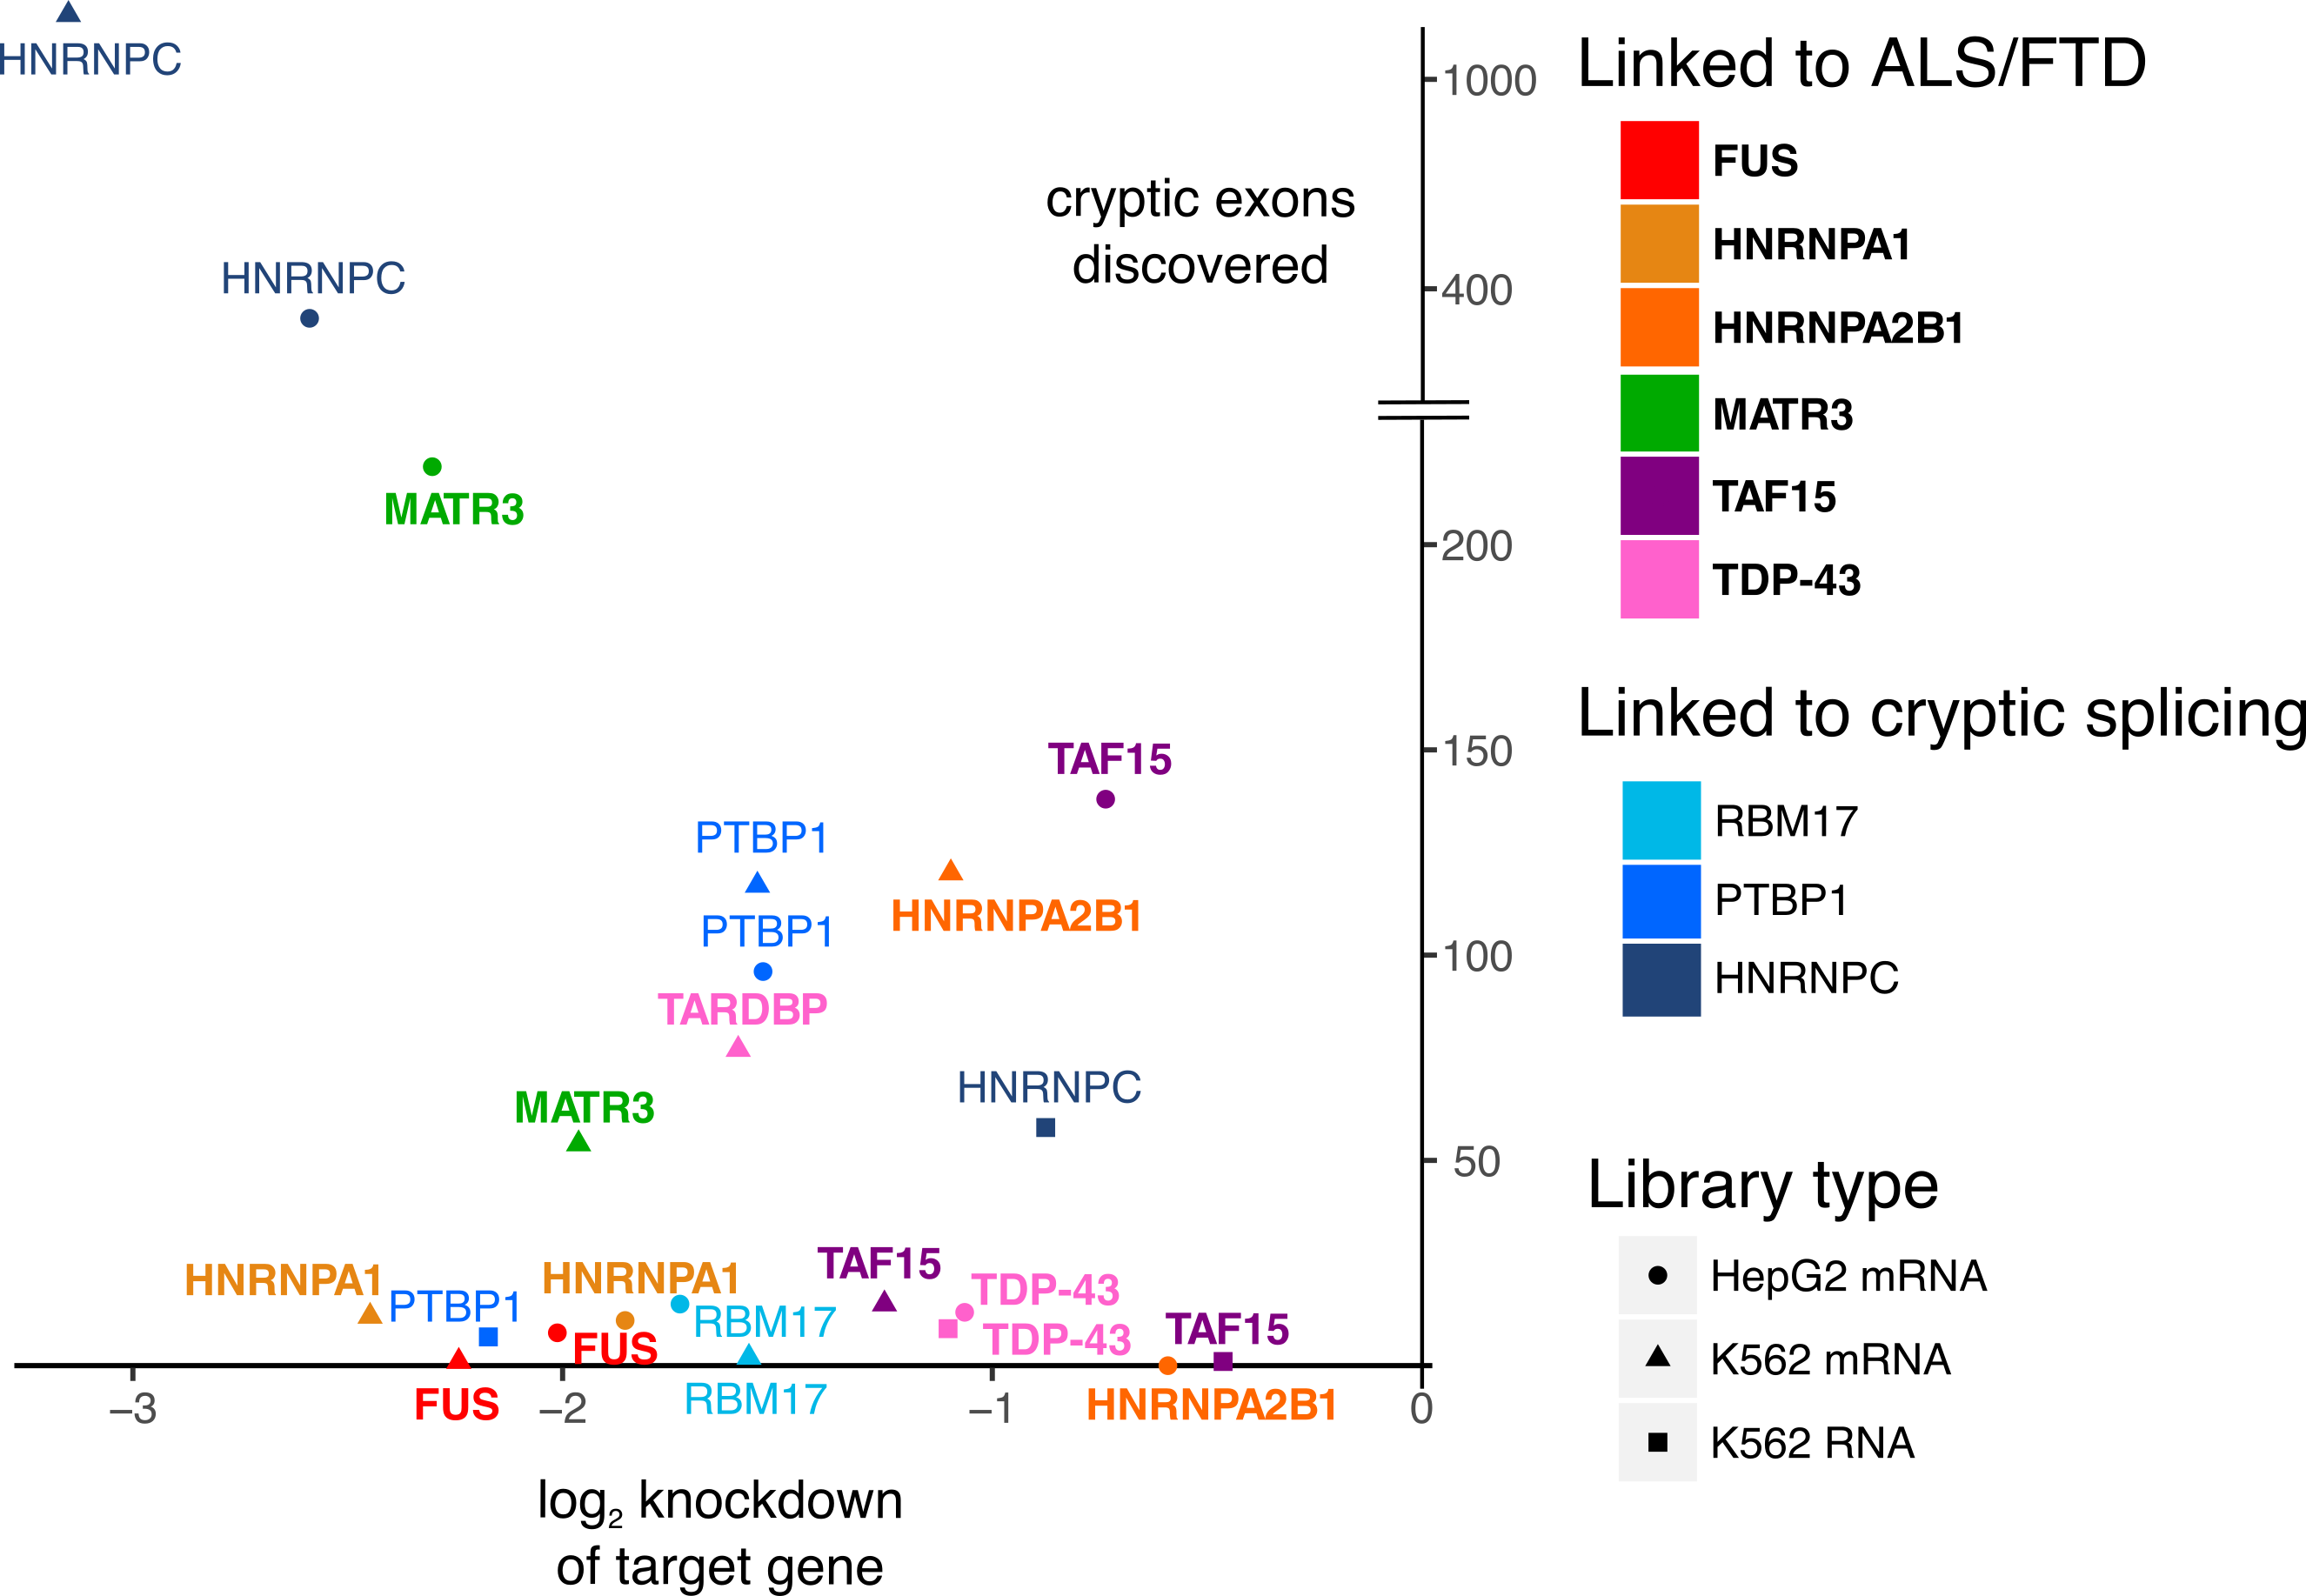
\includegraphics[width=12cm]{Figures/misc/ENCODE_summary.png}
%	\end{center}
%	\caption{ALS and cryptic splicing linked protein knockdowns from the ENCODE consortium  }
%\end{figure} 
%
%\section{Cryptic splicing in ALS and FTD patient brain}
%The initial paper on TDP-43 and cryptic splicing observed that two cryptic exons out of the 50 observed in HeLa cells could also be observed in the brains of ALS patients but not in non-neurological disease controls \citep{Ling2015}. Since then no further work has studied cryptic splicing in ALS or FTD brains. There are multiple lines of evidence that suggest that a number of RNA-binding proteins are perturbed in ALS/FTD as well as TDP-43 and FUS. Therefore if all the potential cryptic targets were known for a host of RNA binding proteins, the inclusion of these cryptic exons in diseased brain would suggest a perturbation in expression of that protein. 
%Building on the results of the TDP-43 cryptic splicing project and the results of the ENCODE screen, I want to thoroughly search for evidence of cryptic splicing in a set of control and disease brains. One such set of sporadic and familial ALS brain RNA-seq data has been previously published \citep{Prudencio2015}. We also have an in-house set of FTD and control brain RNA-seq (unpublished). The data will need to be very carefully prepared. I will attempt to deconvolute gene expression by cell type to compare the levels of neurons and glial cells in the control and diseased brains, to better understand differences in splicing changes between disease samples. RNA-seq of purified cells is available in mouse \citep{Newman2016} and algorithms for this specific task have been developed \citep{Zhang2014}. This approach has successfully applied to human brains to investigate cell type changes in aging \citep{Soreq2017}. There is also scope to look in patient blood and cerebrospinal fluid for potential RNA biomarkers to track disease course. 
%
%\section{Conclusions}
%My work so far has investigated RNA regulation in models of both sporadic and genetic ALS/FTD. Completion of my PhD should result in a fuller picture of cryptic splicing as a general mechanism of disease, complemented by a fine-grained analysis of specific mutations in \textit{TARDBP} and \textit{FUS}. Taking these insights into human patient tissue will be challenging but may lead to advances in understanding both ALS and FTD. 
%




% BIBLIOGRAPHY

\bibliographystyle{Bibliography/plainnat_edit}
\bibliography{Bibliography/thesis_references} %.bib files

% APPENDICES!!!

%
\begin{appendices}
\clearpage	

%% APPENDICES

\section*{Appendices to \autoref{chapter:cryptic_exons} }

\begin{figure}
	\begin{center}
		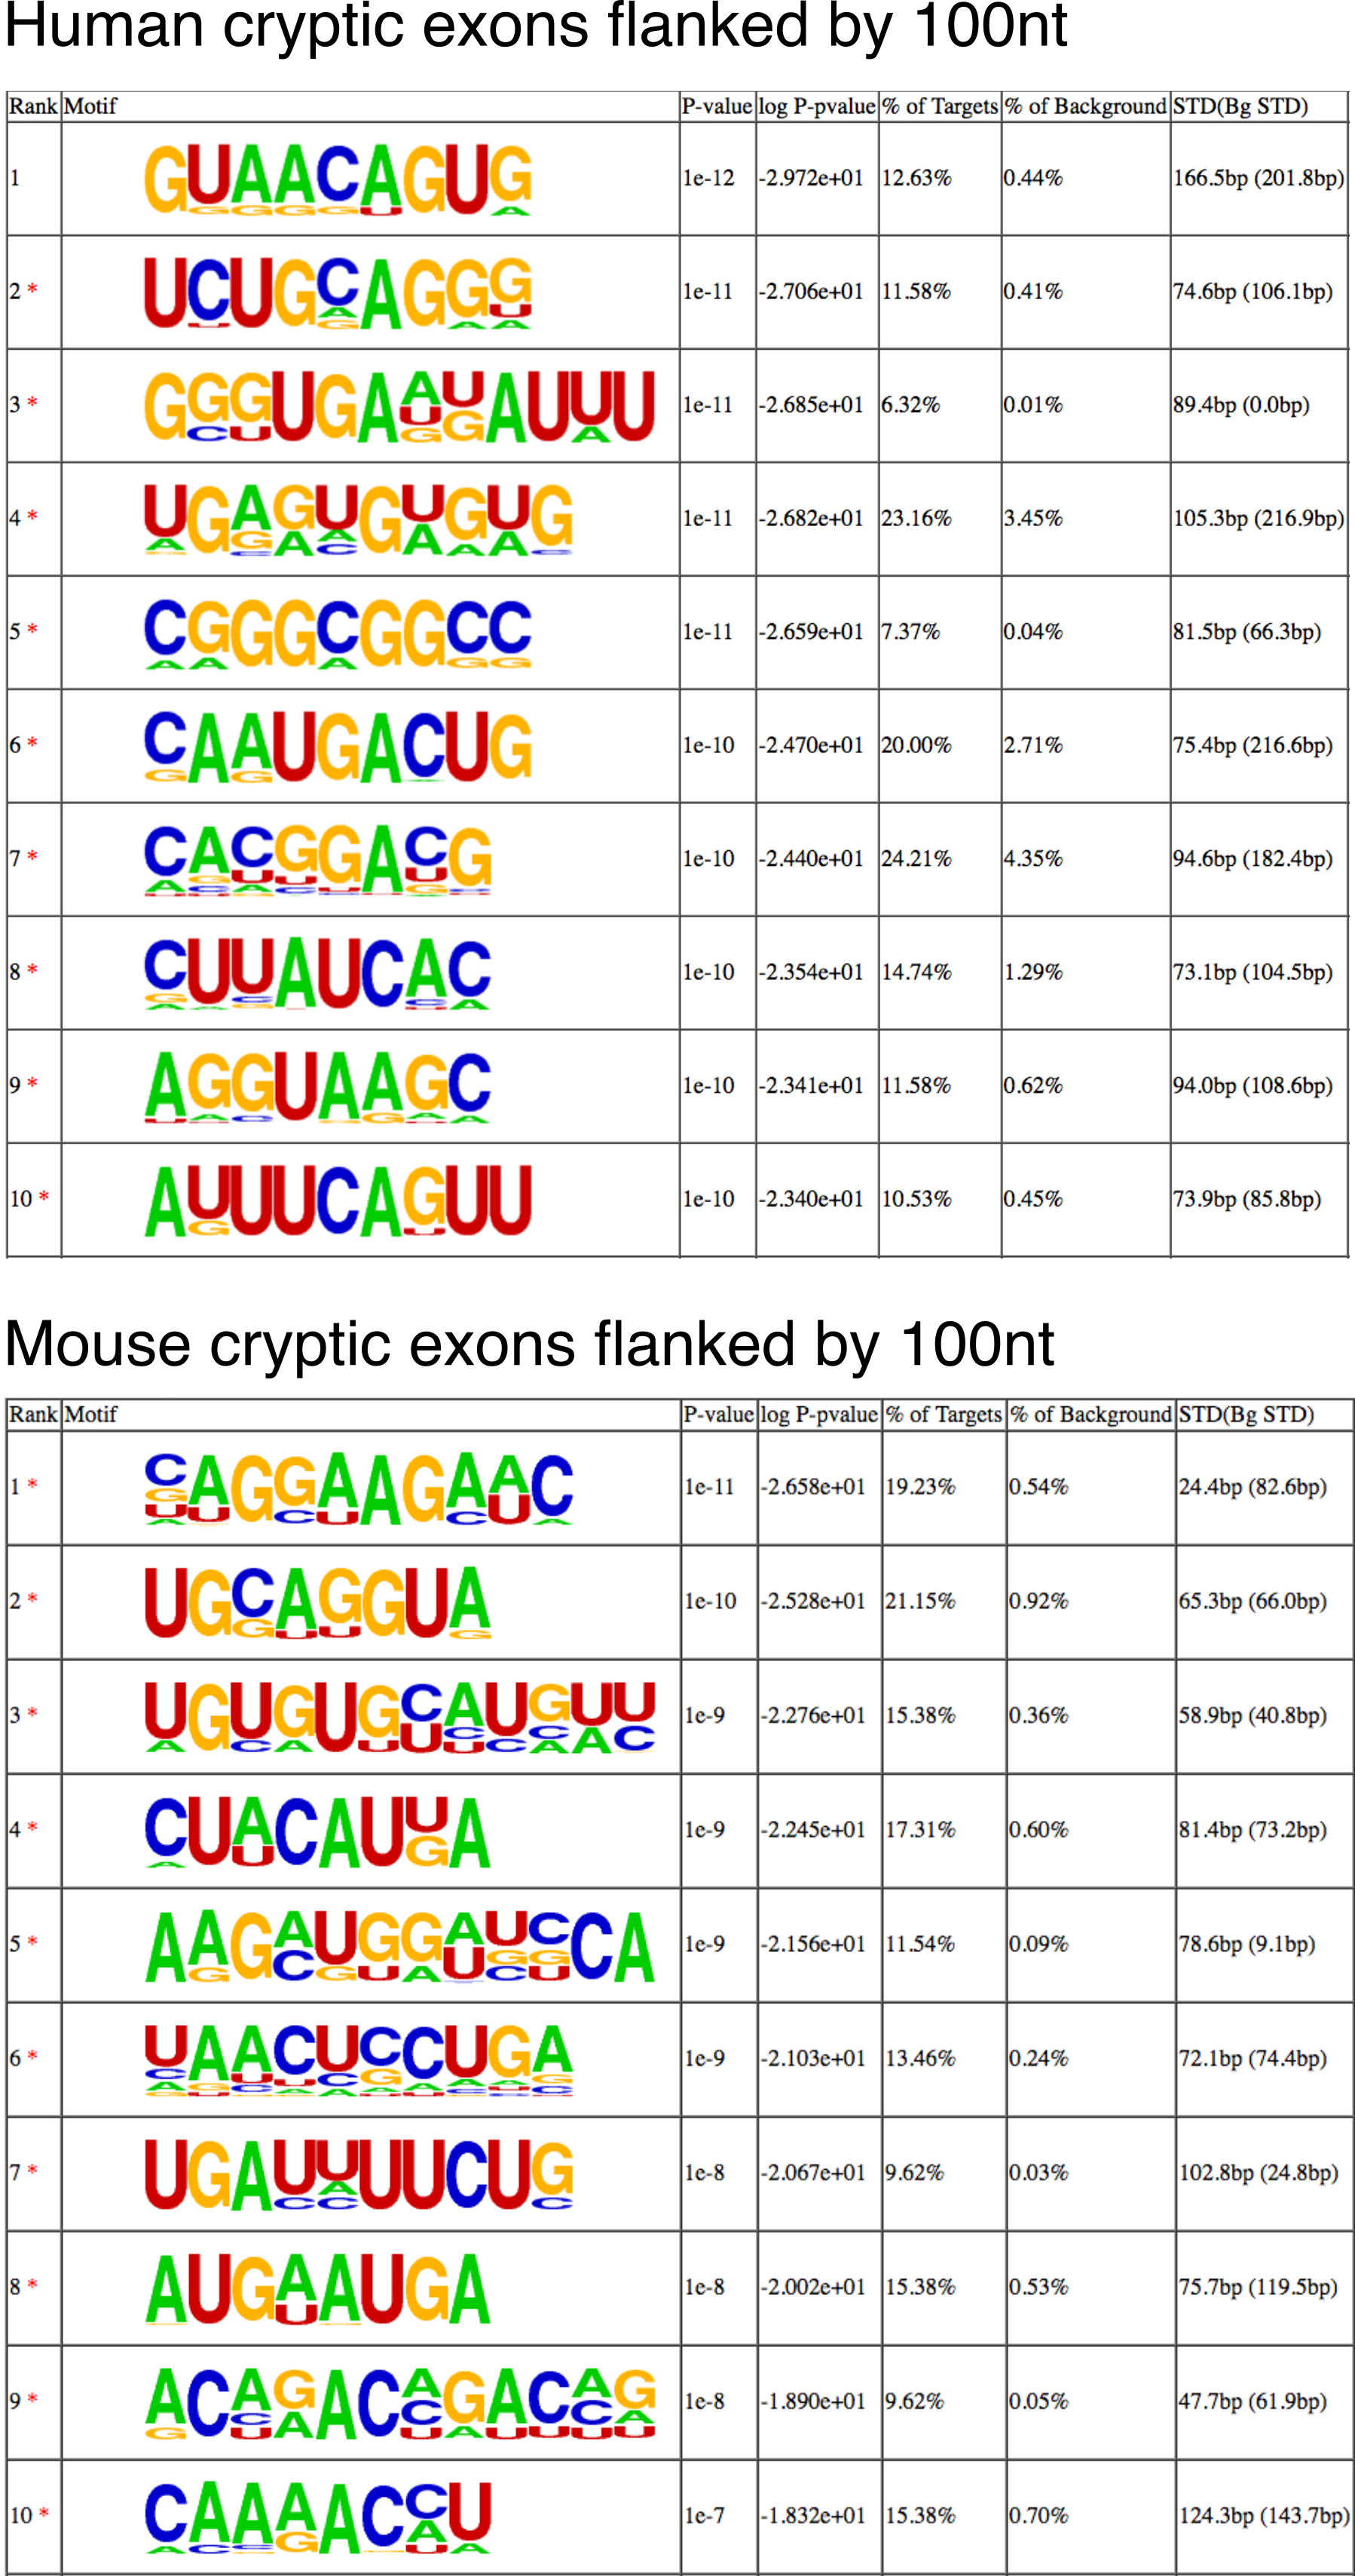
\includegraphics[width=10cm]{Figures/03_cryptic_exons/Figure_S4_HOMER.png}
	\end{center}
	\caption{\textbf{Motifs found by \textit{HOMER}}}
\end{figure}

	\addtolength{\abovecaptionskip}{-25mm}
% mouse table
\newgeometry{left=3cm,bottom=0.8cm}


\begin{landscape}
	%\pagenumbering{gobble}

% Table generated by Excel2LaTeX from sheet 'ST1_mouse_summary_table.tsv'
%\begin{table}[htbp]
% Table generated by Excel2LaTeX from sheet 'ST1_mouse_summary_table.tsv'
\begin{table}[htbp]
	\centering
	2. All mouse cryptic exons discovered by \textit{CryptEx}
	\tiny
	\resizebox{\columnwidth}{!}{
	%\caption{All mouse cryptic exons discovered in chapter 3}
	\begin{tabular}{|l|c|l|l|l|l|c|c|c|l|l|l|l|l|l|}
		\hline
		\multicolumn{15}{|c|}{\cellcolor[HTML]{EFEFEF}{}} \\ \hline
		gene & Ensembl ID & exon ID & chr & exon start & exon end &+/-&5'$\Delta$PSI&3'$\Delta$PSI&classification&observed in&EScell $log_2$FC&brain $log_2$FC&\textit{phyloP}&prediction\\
		\hline
		\textit{Abr} & ENSMUSG00000017631 & E026i1 & chr11 & 76468524 & 76468676 & -     & 0.09  & 0.00  & 5' extension & EScell;brain & -1.75 & -0.59 & 0.77  & PTC/frame shifted \\ \hline
		\textit{Pnpla6} & ENSMUSG00000004565 & E016i1 & chr8  & 3524947 & 3525140 & +     & 0.29  & 0.00  & 5' extension & brain & -1.56 & -0.47 & 0.08  & PTC/frame shifted \\ \hline
		\textit{Lrrc49} & ENSMUSG00000047766 & E017i3 & chr9  & 60637648 & 60637695 & -     & 0.06  & 0.00  & 5' extension & brain & -1.19 & -0.25 & 0.17  & PTC/frame shifted \\ \hline
		\textit{Ccdc149} & ENSMUSG00000045790 & E009i3 & chr5  & 52434250 & 52434424 & -     & 0.16  & 0.00  & 5' extension & brain & .     & -0.28 & 0.06  & PTC/frame conserved \\ \hline
		\textit{Ak5} & ENSMUSG00000039058 & E014i6 & chr3  & 152643869 & 152643915 & -     & 0.16  & 0.00  & 5' extension & brain & .     & -0.53 & 0.17  & PTC/frame shifted \\ \hline
		\textit{Kctd10} & ENSMUSG00000001098 & E017i2 & chr5  & 114376677 & 114376866 & -     & 0.07  & 0.01  & 5' extension & brain & .     & .     & 0.02  & PTC/frame shifted \\ \hline
		\textit{Tmem14a} & ENSMUSG00000025933 & E005i1 & chr1  & 21229121 & 21229173 & +     & 0.37  & 0.00  & 5' extension & brain & -1.02 & -0.60 & -0.08 & PTC/frame conserved \\ \hline
		\textit{Apod} & ENSMUSG00000022548 & E006i1 & chr16 & 31298051 & 31298471 & -     & 0.04  & 0.08  & 3' extension & brain & .     & 0.74  & 0.09  & PTC/frame shifted \\ \hline
		\textit{Erbb2ip} & ENSMUSG00000021709 & E026i1 & chr13 & 103862527 & 103862588 & -     & 0.00  & 0.25  & 3' extension & brain & .     & 0.62  & -0.05 & PTC/frame shifted \\ \hline
		\textit{Trim8} & ENSMUSG00000025034 & E001i2 & chr19 & 46506869 & 46506928 & +     & 0.00  & 0.10  & 3' extension & Ling;brain & .     & .     & -0.23 & PTC/frame shifted \\ \hline
		\textit{Usp15} & ENSMUSG00000099088 & E015i3 & chr10 & 123150961 & 123151125 & -     & 0.00  & 0.32  & 3' extension & Ling;brain & .     & .     & 0.15  & PTC/frame conserved \\ \hline
		\textit{Fam135a} & ENSMUSG00000026153 & E008i1 & chr1  & 24022506 & 24022670 & -     & 0.00  & 0.25  & 3' extension & brain & .     & .     & 0.00  & PTC/frame shifted \\ \hline
		\textit{Rasal1} & ENSMUSG00000029602 & E007i1 & chr5  & 120653508 & 120653879 & +     & 0.03  & 0.16  & 3' extension & brain & .     & .     & -0.23 & PTC/frame conserved \\ \hline
		\textit{Brms1l} & ENSMUSG00000012076 & E008i1 & chr12 & 55864624 & 55865091 & +     & 0.04  & 0.23  & 3' extension & brain & -0.81 & .     & 0.14  & PTC/frame conserved \\ \hline
		\textit{Cacna1b} & ENSMUSG00000004113 & E050i1 & chr2  & 24691959 & 24692366 & -     & 0.00  & 0.39  & 3' extension & brain & .     & -0.58 & 0.21  & PTC/frame shifted \\ \hline
		\textit{Nt5c3b} & ENSMUSG00000017176 & E010i1 & chr11 & 100433637 & 100433684 & -     & 0.00  & 0.07  & 3' extension & brain & -1.15 & -0.50 & 0.12  & PTC/frame conserved \\ \hline
		\textit{Spcs2} & ENSMUSG00000035227 & E004i1 & chr7  & 99856412 & 99856514 & -     & 0.01  & 0.29  & 3' extension & Ling;EScell;brain & .     & 0.34  & 0.40  & PTC/frame shifted \\ \hline
		\textit{Ccdc88a} & ENSMUSG00000032740 & E004i8 & chr11 & 29421354 & 29421401 & +     & 0.00  & 0.27  & 3' extension & brain & -1.63 & .     & -0.04 & PTC/frame conserved \\ \hline
		\textit{Adap1} & ENSMUSG00000056413 & E014i3 & chr5  & 139302108 & 139302166 & -     & 0.00  & 0.36  & 3' extension & brain & .     & -0.47 & 0.08  & PTC/frame shifted \\ \hline
		\textit{Ap3b2} & ENSMUSG00000062444 & E031i2 & chr7  & 81490178 & 81490277 & -     & 0.04  & 0.10  & 3' extension & brain & 0.50  & -0.28 & 0.18  & PTC/frame shifted \\ \hline
		\textit{Fam73a} & ENSMUSG00000054942 & E015i2 & chr3  & 152292556 & 152292657 & -     & 0.02  & 0.09  & 3' extension & Ling;brain & -1.39 & -0.63 & -0.04 & PTC/frame shifted \\ \hline
		\textit{Ptprn2} & ENSMUSG00000056553 & E019i11 & chr12 & 117154249 & 117154298 & +     & 0.00  & 0.13  & 3' extension & brain & .     & -1.01 & 0.24  & PTC/frame shifted \\ \hline
		\textit{Dlg2} & ENSMUSG00000052572 & E004i17 & chr7  & 91543136 & 91543191 & +     & 0.00  & 0.23  & 3' extension & brain & .     & -0.71 & 1.67  & PTC/frame shifted \\ \hline
		\textit{Cd200} & ENSMUSG00000022661 & E003i1 & chr16 & 45389970 & 45390184 & -     & 0.04  & 0.06  & 3' extension & brain & .     & .     & -0.13 & Not in CDS \\ \hline
		\textit{Dock4} & ENSMUSG00000035954 & E049i1 & chr12 & 40835769 & 40835912 & +     & 0.09  & 0.20  & Cassette & brain & .     & -0.68 & 0.53  & PTC/frame shifted \\ \hline
		\textit{C4b} & ENSMUSG00000073418 & E032i1 & chr17 & 34739389 & 34739500 & -     & 0.06  & 0.30  & Cassette & brain & .     & .     & 0.00  & PTC/frame shifted \\ \hline
		\textit{Camk1g} & ENSMUSG00000016179 & E017i2 & chr1  & 193368866 & 193368952 & -     & 0.70  & 0.47  & Cassette & brain & .     & .     & -0.06 & Not in CDS  \\ \hline
		\textit{Reep3} & ENSMUSG00000019873 & E001i1 & chr10 & 67014087 & 67014164 & -     & 0.67  & 0.39  & Cassette & brain & .     & 0.44  & -0.01 & PTC/frame shifted \\ \hline
		\textit{Drosha} & ENSMUSG00000022191 & E009i1 & chr15 & 12833221 & 12833389 & +     & 0.10  & 0.15  & Cassette & brain & .     & .     & -0.06 & PTC/frame conserved \\ \hline
		\textit{Synj2bp} & ENSMUSG00000021139 & E036i2 & chr12 & 81509671 & 81510249 & -     & 0.41  & 0.07  & Cassette & brain & .     & .     & 0.11  & PTC/frame shifted \\ \hline
		\textit{Adnp2} & ENSMUSG00000053950 & E002i1 & chr18 & 80138152 & 80138304 & -     & 0.57  & 0.50  & Cassette & Ling;EScell;brain & 0.33  & 0.25  & 0.03  & PTC/frame shifted \\ \hline
		\textit{Adipor2} & ENSMUSG00000030168 & E010i2 & chr6  & 119369859 & 119369918 & -     & 0.30  & 0.44  & Cassette & Ling;brain & -1.06 & .     & 0.07  & PTC/frame shifted \\ \hline
		\textit{Cdh22} & ENSMUSG00000053166 & E013i2 & chr2  & 165183238 & 165183371 & -     & 0.40  & 0.67  & Cassette & brain & .     & -0.35 & 0.13  & Not in CDS \\ \hline
		\textit{Ermn} & ENSMUSG00000026830 & E001i1 & chr2  & 58049485 & 58049561 & -     & 0.16  & 0.16  & Cassette & brain & .     & .     & 0.06  & PTC/frame shifted \\ \hline
		\textit{Ift81} & ENSMUSG00000029469 & E003i1 & chr5  & 122556905 & 122556991 & -     & 0.19  & 0.08  & Cassette & Ling;brain & .     & .     & 0.08  & benign/frame shifted \\ \hline
		\textit{Vps13d} & ENSMUSG00000020220 & E043i1 & chr4  & 145099351 & 145099463 & -     & 0.60  & 0.20  & Cassette & brain & .     & -0.81 & 0.23  & PTC/frame shifted \\ \hline
		\textit{Ube2d1} & ENSMUSG00000019927 & E010i1 & chr10 & 71263584 & 71263717 & -     & 0.15  & 0.36  & Cassette & EScell;brain & .     & 0.35  & 0.04  & PTC/frame shifted \\ \hline
		\textit{Hgsnat} & ENSMUSG00000037260 & E001i1 & chr8  & 25945947 & 25945999 & -     & 0.28  & 0.15  & Cassette & Ling;brain & -0.59 & .     & 0.20  & PTC/frame conserved \\ \hline
		\textit{Elmod1} & ENSMUSG00000041986 & E003i2 & chr9  & 53923941 & 53923995 & -     & 0.27  & 0.19  & Cassette & brain & .     & .     & 0.97  & benign/frame conserved \\ \hline
		\textit{Mkx} & ENSMUSG00000061013 & E007i7 & chr18 & 6986138 & 6986235 & -     & 0.24  & 0.50  & Cassette & brain & .     & .     & -0.08 & PTC/frame shifted \\ \hline
		\textit{Hace1} & ENSMUSG00000038822 & E013i1 & chr10 & 45639722 & 45639803 & +     & 0.06  & 0.20  & Cassette & Ling;brain & .     & -0.38 & 0.10  & benign/frame conserved \\ \hline
		\textit{Fxyd2} & ENSMUSG00000059412 & E003i1 & chr9  & 45408987 & 45409173 & +     & 0.42  & 0.18  & Cassette & brain & -1.89 & .     & -0.25 & PTC/frame shifted \\ \hline
		\textit{Thoc7} & ENSMUSG00000053453 & E007i1 & chr14 & 13957061 & 13957631 & -     & 0.21  & -0.10 & 5' extension & EScell & -0.74 & .     & 0.04  & PTC/frame shifted \\ \hline
		\textit{Nme6} & ENSMUSG00000032478 & E020i1 & chr9  & 109837872 & 109838225 & +     & 0.40  & 0.00  & 5' extension & Ling;EScell & -0.84 & .     & 0.21  & PTC/frame conserved \\ \hline
		\textit{Wtip} & ENSMUSG00000036459 & E001i1 & chr7  & 34111074 & 34111099 & -     & 0.13  & 0.00  & 5' extension & EScell & -0.46 & .     & 0.26  & PTC/frame shifted \\ \hline
		\textit{Gsta4} & ENSMUSG00000032348 & E005i2 & chr9  & 78207196 & 78207382 & +     & 0.02  & 0.07  & 3' extension & Ling;EScell & -0.45 & .     & 0.11  & PTC/frame shifted \\ \hline
		\textit{Slc7a6} & ENSMUSG00000031904 & E001i1 & chr8  & 106169186 & 106169256 & +     & 0.00  & 0.12  & 3' extension & EScell & .     & -0.23 & -0.25 & Not in CDS \\ \hline
		\textit{Flnb} & ENSMUSG00000025278 & E040i1 & chr14 & 7935368 & 7935630 & +     & 0.09  & 0.43  & Cassette & Ling;EScell;brain & -1.34 & .     & -0.12 & PTC/frame shifted \\ \hline
		\textit{B4galnt3} & ENSMUSG00000041372 & E002i1 & chr6  & 120204263 & 120204465 & -     & 0.07  & 0.10  & Cassette & EScell & .     & .     & -0.15 & PTC/frame shifted \\ \hline
		\textit{Psma2} & ENSMUSG00000015671 & E005i1 & chr13 & 14620930 & 14621038 & +     & 0.06  & 0.13  & Cassette & EScell & .     & .     & 0.19  & PTC/frame conserved \\ \hline
		\textit{Abr} & ENSMUSG00000017631 & E024i1 & chr11 & 76464580 & 76464758 & -     & 0.18  & 0.07  & Cassette & EScell;brain & -1.75 & -0.59 & -0.25 & PTC/frame shifted \\ \hline
		\textit{Wasf3} & ENSMUSG00000029636 & E009i1 & chr5  & 146469766 & 146469912 & +     & 0.10  & 0.22  & Cassette & EScell & .     & .     & -0.02 & benign/frame conserved \\ \hline
	\end{tabular}%
	}
\end{table}%

\clearpage

\begin{table}
	\centering
	3. All human cryptic exons discovered by \textit{CryptEx}
	\tiny
	\resizebox{\columnwidth}{!}{ 
%	\fontsize{5}{6}
	\begin{tabular}{|l|c|l|l|l|l|c|c|c|l|l|l|l|l|l|l|l|}
		\hline
%		\multicolumn{17}{Human cryptic exons} \\ 
		\multicolumn{17}{|c|}{\cellcolor[HTML]{EFEFEF}{} } \\ 
		\hline
		gene&Ensembl ID&exon ID&chr&exon start&exon end&+/-& 5'$\Delta$PSI&3'$\Delta$PSI& classification& observed in &mRNA FC&total FC&\textit{phyloP}&prediction&\textit{maxEnt} 5'&\textit{maxEnt} 3'\\ \hline 
		\textit{PHF12} & ENSG00000109118 & E028i1 & chr17 & 28914903 & 28915475 & -     & 0.14  & 0.00  & 5' extension & mRNA;total & 0.23  & . & 0.448493 & PTC/frame conserved & . &  9.93 \\ \hline
		\textit{ZFPM2} & ENSG00000169946 & E016i1 & chr8  & 105419822 & 105419906 & +     & 0.35  & 0.00  & 5' extension & mRNA  & . & . & -0.131815 & PTC/frame conserved & . &  11.28 \\ \hline
		\textit{ACBD3} & ENSG00000182827 & E004i1 & chr1  & 226156701 & 226156780 & -     & 0.12  & 0.00  & 5' extension & mRNA  & -0.31 & . & 0.22671 & PTC/frame shifted & . &  9.63 \\ \hline
		\textit{RPS6KA3} & ENSG00000177189 & E031i2 & chrX  & 20241592 & 20241686 & -     & 0.18  & 0.01  & 5' extension & mRNA  & -0.42 & . & 2.38738 & PTC/frame shifted & . &  8.09 \\ \hline
		\textit{CPED1} & ENSG00000106034 & E034i7 & chr7  & 121194471 & 121194593 & +     & 0.07  & 0.01  & 5' extension & mRNA  & . & . & 0.398074 & PTC/frame shifted & . &  9.56 \\ \hline
		\textit{HUWE1} & ENSG00000086758 & E033i1 & chrX  & 53551990 & 53552074 & -     & 0.09  & 0.05  & 5' extension & mRNA  & -0.56 & . & 0.114241 & PTC/frame shifted & . &  6.87 \\ \hline
		\textit{DYNC2LI1} & ENSG00000138036 & E006i1 & chr2  & 43774402 & 43774936 & +     & 0.08  & 0.04  & 5' extension & mRNA  & -0.63 & . & -0.228969 & PTC/frame shifted & . &  2.09 \\ \hline
		\textit{ZMYND8} & ENSG00000101040 & E019i2 & chr20 & 47254235 & 47254424 & -     & 0.07  & 0.03  & 5' extension & mRNA  & -0.36 & . & 0.101961 & PTC/frame shifted & . &  3.77 \\ \hline
		\textit{HEPH} & ENSG00000089472 & E030i1 & chrX  & 66257344 & 66257516 & +     & 0.12  & 0.00  & 5' extension & mRNA  & -0.58 & -0.34 & 0.245606 & PTC/frame shifted & . &  14.19 \\ \hline
		\textit{BTNL9} & ENSG00000165810 & E031i1 & chr5  & 181059149 & 181059215 & +     & 0.09  & 0.00  & 5' extension & mRNA  & . & . & -0.101275 & PTC/frame shifted & . &  -0.66 \\ \hline
		\textit{PAPSS1} & ENSG00000138801 & E008i1 & chr4  & 107654948 & 107655036 & -     & 0.08  & 0.00  & 5' extension & mRNA;total & -0.87 & . & 0.746813 & PTC/frame conserved & . &  10.84 \\ \hline
		\textit{CLASP1} & ENSG00000074054 & E049i1 & chr2  & 121471187 & 121471274 & -     & 0.16  & 0.00  & 5' extension & mRNA  & -0.19 & . & -0.0460715 & PTC/frame shifted & . &  4.56 \\ \hline
		\textit{IST1} & ENSG00000224470 & E053i1 & chr16 & 71922108 & 71922437 & +     & 0.12  & 0.01  & 5' extension & mRNA  & . & . & 0.177172 & PTC/frame shifted & . &  13.96 \\ \hline
		\textit{UBR4} & ENSG00000272084& E084i1 & chr1  & 19145598 & 19145708 & -     & 0.05  & 0.00  & 5' extension & mRNA  & . & . & 0.710974 & PTC/frame shifted & . &  7.28 \\ \hline
		\textit{ANKRD27} & ENSG00000105186 & E019i1 & chr19 & 32630070 & 32630151 & -     & 0.15  & 0.01  & 5' extension & mRNA  & -0.37 & -0.24 & -0.103821 & PTC/frame shifted & . &  12.52 \\ \hline
		\textit{CCDC77} & ENSG00000120647 & E020i1 & chr12 & 422421 & 422891 & +     & 0.07  & 0.01  & 5' extension & mRNA  & -0.84 & . & -0.0231545 & PTC/frame shifted & . &  3.79 \\ \hline
		\textit{LRPPRC} & ENSG00000138095 & E024i1 & chr2  & 43942675 & 43942815 & -     & 0.06  & 0.00  & 5' extension & mRNA  & -1.01 & . & 0.14133 & PTC/frame shifted & . &  3.85 \\ \hline
		\textit{ADGRV1} & ENSG00000164199 & E085i1 & chr5  & 90803514 & 90803596 & +     & 0.07  & 0.00  & 5' extension & mRNA  & -0.47 & 0.32  & -0.185377 & PTC/frame shifted & . &  9.14 \\ \hline
		\textit{ASNSP1} & ENSG00000248498 & E006i1 & chr8  & 46595259 & 46595315 & -     & 0.13  & 0.00  & 5' extension & mRNA  & . & . & 1.14798 & Not in CDS     & . &  8.29 \\ \hline
		\textit{SMAD2} & ENSG00000175387 & E010i1 & chr18 & 47868051 & 47868103 & -     & 0.08  & 0.02  & 5' extension & mRNA  & -0.39 & . & 0.289826 & PTC/frame shifted & . &  9.95 \\ \hline
		\textit{ZNHIT6} & ENSG00000117174 & E003i1 & chr1  & 85662210 & 85662278 & -     & 0.08  & 0.04  & 5' extension & mRNA  & -0.80 & . & 0.0230322 & PTC/frame conserved & . &  5.75 \\ \hline
		\textit{NLRP1} & ENSG00000091592 & E045i1 & chr17 & 5585499 & 5585635 & -     & 0.15  & 0.00  & 5' extension & mRNA  & . & . & -0.1356 & Not in CDS     & . &  5.48 \\ \hline
		\textit{CEP290} & ENSG00000198707 & E024i1 & chr12 & 88086709 & 88086789 & -     & 0.13  & 0.00  & 5' extension & mRNA  & -1.15 & . & 0.157693 & PTC/frame shifted & . &  7.83 \\ \hline
		\textit{METTL8} & ENSG00000123600 & E037i1 & chr2  & 171433562 & 171433649 & -     & 0.50  & 0.00  & 5' extension & mRNA  & . & . & 0.223589 & Not in CDS     & . &  11.06 \\ \hline
		\textit{MPDZ} & ENSG00000107186 & E015i1 & chr9  & 13110935 & 13111024 & -     & 0.35  & 0.00  & 5' extension & mRNA  & -0.57 & . & 0.11092 & PTC/frame shifted & . &  10.52 \\ \hline
		\textit{ERBB2IP} & ENSG00000112851 & E013i2 & chr5  & 65997127 & 65997228 & +     & 0.06  & 0.04  & 5' extension & mRNA  & -0.39 & . & 0.211071 & PTC/frame shifted & . &  9.62 \\ \hline
		\textit{PRPF40A} & ENSG00000196504 & E001i1 & chr2  & 152657053 & 152657141 & -     & 0.04  & 0.05  & 3' extension & mRNA  & -0.77 & . & -0.0653744 & PTC/frame shifted & -0.49 & . \\ \hline
		\textit{UPF2} & ENSG00000151461 & E002i1 & chr10 & 11926921 & 11927006 & -     & 0.00  & 0.16  & 3' extension & Ling;mRNA & . & . & 0.00227976 & PTC/frame shifted & 9.85  & . \\ \hline
		\textit{RRP1} & ENSG00000160214 & E008i1 & chr21 & 43791522 & 43792578 & +     & 0.02  & 0.08  & 3' extension & mRNA  & 0.82  & . & -0.184698 & PTC/frame shifted & 6.51  & . \\ \hline
		\textit{LRP8} & ENSG00000157193 & E033i1 & chr1  & 53274090 & 53274694 & -     & 0.00  & 0.27  & 3' extension & mRNA;total & . & . & 1.77583 & PTC/frame conserved & 2.70  & . \\ \hline
		\textit{PKP4} & ENSG00000144283 & E020i1 & chr2  & 158588958 & 158588987 & +     & 0.00  & 0.17  & 3' extension & mRNA  & -0.31 & . & 0.0933565 & PTC/frame shifted & 3.91  & . \\ \hline
		\textit{DDX52} & ENSG00000278053 & E022i1 & chr17 & 37629848 & 37629963 & -     & 0.01  & 0.08  & 3' extension & mRNA;total & -0.39 & -0.30 & 0.981172 & PTC/frame conserved & 7.96  & . \\ \hline
		\textit{SETD5} & ENSG00000168137 & E065i1 & chr3  & 9468576 & 9468615 & +     & 0.00  & 0.13  & 3' extension & Ling;mRNA;total & -0.24 & . & 2.57544 & PTC/frame conserved & 7.36  & . \\ \hline
		\textit{KDELC2} & ENSG00000178202 & E018i2 & chr11 & 108497751 & 108498085 & -     & 0.00  & 0.19  & 3' extension & Ling;mRNA & -0.78 & . & -0.0860609 & PTC/frame conserved & 8.95  & . \\ \hline
		\textit{GPT2} & ENSG00000166123 & E009i1 & chr16 & 46900812 & 46900883 & +     & 0.00  & 0.16  & 3' extension & mRNA  & -0.98 & -0.72 & 1.01736 & PTC/frame shifted & 3.30  & . \\ \hline
		\textit{GSE1} & ENSG00000131149 & E007i1 & chr16 & 85650416 & 85650709 & +     & 0.04  & 0.06  & 3' extension & mRNA  & 0.29  & . & -0.525771 & PTC/frame shifted & 5.99  & . \\ \hline
		\textit{MBOAT2} & ENSG00000143797 & E029i2 & chr2  & 8986052 & 8986136 & -     & 0.00  & 0.25  & 3' extension & mRNA  & -0.66 & . & -0.0138646 & PTC/frame shifted & 8.34  & . \\ \hline
		\textit{DNAAF5} & ENSG00000164818 & E024i1 & chr7  & 783225 & 783309 & +     & 0.00  & 0.05  & 3' extension & mRNA  & 0.49  & -0.37 & -0.238231 & PTC/frame shifted & 9.25  & . \\ \hline
		\textit{CLASP1} & ENSG00000074054 & E012i1 & chr2  & 121387587 & 121387655 & -     & 0.04  & 0.07  & 3' extension & mRNA  & -0.19 & . & -0.0066914 & PTC/frame conserved & 2.72  & . \\ \hline
		\textit{ZFP91} & ENSG00000255073 & E012i1 & chr11 & 58616974 & 58617182 & +     & 0.04  & 0.05  & 3' extension & mRNA  & . & . & -0.213922 & PTC/frame shifted & 6.97  & . \\ \hline
		\textit{FAM178B} & ENSG00000273634 & E017i1 & chr2  & 96923867 & 96924228 & -     & 0.00  & 0.30  & 3' extension & mRNA  & . & . & -0.351309 & PTC/frame shifted & 3.14  & . \\  \hline
		\textit{ANAPC1} & ENSG00000153107 & E020i1 & chr2  & 111799529 & 111799699 & -     & 0.00  & 0.12  & 3' extension & mRNA  & -0.90 & . & 0.0276639 & PTC/frame conserved & 5.28  & . \\ \hline
		\textit{CERK} & ENSG00000100422 & E005i1 & chr22 & 46691869 & 46692022 & -     & 0.03  & 0.14  & 3' extension & mRNA  & . & . & -0.579144 & PTC/frame shifted & 9.22  & . \\ \hline
		\textit{ARHGAP11B} & ENSG00000187951 & E033i1 & chr15 & 30755981 & 30756067 & +     & 0.00  & 0.11  & 3' extension & mRNA  & . & . & -0.13533 & Not in CDS     & 10.77 & . \\ \hline
		\textit{GOLGA8A} & ENSG00000175265 & E037i1 & chr15 & 34436658 & 34436837 & -     & 0.00  & 0.10  & 3' extension & mRNA  & -0.58 & . & -0.147737 & Not in CDS     & 8.72  & . \\ \hline
		\textit{TGFBRAP1} & ENSG00000135966 & E014i2 & chr2  & 105307479 & 105307570 & -     & 0.00  & 0.19  & 3' extension & mRNA  & . & . & 0.807447 & PTC/frame shifted & 4.75  & . \\ \hline
		\textit{CAMK2G} & ENSG00000148660 & E039i1 & chr10 & 73873200 & 73873283 & -     & 0.00  & 0.21  & 3' extension & mRNA  & . & . & 0.336877 & PTC/frame shifted & 6.32  & . \\ \hline
	\end{tabular}
	}
\end{table}	
\begin{table}
	\centering
	3. All human cryptic exons discovered by \textit{CryptEx} (continued)
	\tiny
	\resizebox{\columnwidth}{!}{ 
	\begin{tabular}{|l|c|l|l|l|l|c|c|c|l|l|l|l|l|l|l|l|}
		\hline
		\multicolumn{17}{|c|}{\cellcolor[HTML]{EFEFEF}{ } } \\ 
		\hline
		gene&Ensembl ID&exon ID&chr&exon start&exon end&+/-& 5'$\Delta$PSI&3'$\Delta$PSI& classification& observed in &mRNA FC&total FC&\textit{phyloP}&prediction&\textit{maxEnt} 5'&\textit{maxEnt} 3'\\ \hline 
		\textit{DCAF17} & ENSG00000115827 & E008i1 & chr2  & 171441954 & 171442195 & +     & 0.04  & 0.07  & 3' extension & mRNA  & -0.50 & . & 0.207598 & PTC/frame conserved & 5.13  & . \\ \hline
		\textit{RP1-179N16.6} & ENSG00000246982 & E002i2 & chr6  & 36160683 & 36160784 & -     & 0.02  & 0.13  & 3' extension & mRNA  & . & . & 0.161445 & Not in CDS     & 9.16  & . \\ \hline
		\textit{RNFT2} & ENSG00000135119 & E016i2 & chr12 & 116790033 & 116790087 & +     & 0.00  & 0.15  & 3' extension & Ling;mRNA & . & . & 0.118938 & PTC/frame shifted & 7.03  & . \\ \hline
		\textit{SH2B3} & ENSG00000111252 & E005i1 & chr12 & 111446092 & 111446216 & +     & 0.00  & 0.11  & 3' extension & mRNA  & . & -0.52 & -0.401417 & PTC/frame shifted & 5.85  & . \\ \hline
		\textit{SENP7} & ENSG00000138468 & E020i1 & chr3  & 101349160 & 101349188 & -     & 0.00  & 0.05  & 3' extension & mRNA  & -1.11 & . & 0.116452 & PTC/frame shifted & 6.06  & . \\ \hline
		\textit{GOLGB1} & ENSG00000173230 & E013i1 & chr3  & 121682916 & 121682980 & -     & 0.03  & 0.08  & 3' extension & mRNA  & -0.40 & 0.26  & 0.918212 & PTC/frame conserved & 9.35  & . \\ \hline
		\textit{AGRN} & ENSG00000242590 & E015i1 & chr1  & 1044440 & 1045080 & +     & 0.46  & 0.63  & Cassette & Ling;mRNA;total & . & . & -0.913282 & PTC/frame shifted & 5.78  &  4.71 \\ \hline
\textit{CEP72} & ENSG00000112877 & E012i1 & chr5  & 648049 & 648223 & +     & 0.69  & 0.70  & Cassette & Ling;mRNA;total & . & -0.30 & -0.102364 & PTC/frame shifted & 9.81  &  -7.11 \\ \hline
\textit{RAP1GAP} & ENSG00000076864 & E010i1 & chr1  & 21598718 & 21598820 & -     & 0.27  & 0.34  & Cassette & mRNA  & . & -0.39 & -0.293165 & PTC/frame shifted & 6.51  &  7.06 \\ \hline
\textit{PFKP} & ENSG00000067057 & E010i1 & chr10 & 3099556 & 3099819 & +     & 0.29  & 0.19  & Cassette & Ling;mRNA;total & . & . & -0.0943177 & PTC/frame shifted & 4.88  &  2.02 \\ \hline
\textit{PKN1} & ENSG00000123143 & E016i2 & chr19 & 14450087 & 14450214 & +     & 0.22  & 0.10  & Cassette & Ling;mRNA & . & -0.49 & 0.0079453 & PTC/frame shifted & 4.88  &  6.94 \\ \hline
\textit{FAM114A2} & ENSG00000055147 & E040i1 & chr5  & 154037367 & 154037457 & -     & 0.27  & 0.23  & Cassette & Ling;mRNA;total & . & . & 0.205094 & Not in CDS & 8.11  &  11.04 \\ \hline
\textit{HDGFRP2} & ENSG00000167674 & E015i1 & chr19 & 4492012 & 4492152 & +     & 0.15  & 0.10  & Cassette & Ling;mRNA & 0.90  & . & -0.606886 & benign/frame conserved & 6.14  &  7.67 \\ \hline
\textit{PRPF38A} & ENSG00000134748 & E003i1 & chr1  & 52405054 & 52405321 & +     & 0.05  & 0.07  & Cassette & mRNA  & . & . & 0.106102 & PTC/frame conserved & 6.99  &  6.54 \\ \hline
\textit{ATG4B} & ENSG00000168397 & E047i1 & chr2  & 241668874 & 241669149 & +     & 0.10  & 0.24  & Cassette & Ling;mRNA & 0.47  & . & -0.307633 & PTC/frame conserved & 10.13 &  10.45 \\ \hline
\textit{ADSS} & ENSG00000035687 & E020i1 & chr1  & 244433371 & 244433496 & -     & 0.11  & 0.10  & Cassette & mRNA  & . & . & 0.185587 & PTC/frame shifted & 7.83  &  7.65 \\ \hline
\textit{NSUN2} & ENSG00000037474 & E024i1 & chr5  & 6619315 & 6619467 & -     & 0.07  & 0.07  & Cassette & mRNA  & -0.39 & -0.39 & -0.517291 & PTC/frame shifted & 9.14  &  11.12 \\ \hline		
		\textit{TAOK3} & ENSG00000135090 & E007i1 & chr12 & 118151926 & 118151997 & -     & 0.05  & 0.06  & Cassette & mRNA  & . & . & 0.0363395 & PTC/frame conserved & 8.56  &  8.68 \\ \hline
		\textit{CORO7} & ENSG00000103426 & E081i1 & chr16 & 4367297 & 4367729 & -     & 0.25  & 0.10  & Cassette & mRNA  & . & . & -0.121763 & PTC/frame shifted & 3.34  &  5.19 \\ \hline
		\textit{HBG2} & ENSG00000196565 & E016i1 & chr11 & 5258008 & 5258776 & -     & 0.58  & 0.34  & Cassette & mRNA;total & . & . & -0.0145071 & Not in CDS     & 5.91  &  10.53 \\ \hline
		\textit{SSFA2} & ENSG00000138434 & E024i1 & chr2  & 181911125 & 181911233 & +     & 0.23  & 0.22  & Cassette & Ling;mRNA;total & -0.32 & . & 0.0525638 & PTC/frame conserved & 6.69  &  6.70 \\ \hline
		\textit{MAR3} & ENSG00000173926 & E009i1 & chr5  & 126917510 & 126917676 & -     & 0.14  & 0.05  & Cassette & mRNA  & 0.51  & . & 0.178889 & PTC/frame shifted & 3.82  &  7.74 \\ \hline
		\textit{HERC1} & ENSG00000103657 & E014i1 & chr15 & 63629529 & 63629697 & -     & 0.05  & 0.09  & Cassette & mRNA  & -0.74 & -0.31 & 0.164758 & PTC/frame conserved & 3.53  &  4.58 \\ \hline
		\textit{SP3} & ENSG00000172845 & E011i1 & chr2  & 173957233 & 173957376 & -     & 0.08  & 0.20  & Cassette & mRNA  & -0.29 & . & 0.236352 & PTC/frame conserved & 3.78  &  10.06 \\ \hline
		\textit{DDHD1} & ENSG00000100523 & E023i1 & chr14 & 53096116 & 53096218 & -     & 0.21  & 0.42  & Cassette & mRNA  & . & . & 3.39222 & benign/frame conserved & 8.04  &  5.98 \\ \hline
		\textit{RP11-488L18.4} & ENSG00000227671 & E001i4 & chr1  & 247197079 & 247197247 & -     & 0.10  & 0.07  & Cassette & mRNA  & . & . & 0.00769496 & Not in CDS     & 5.17  &  8.01 \\ \hline
		\textit{UHRF2} & ENSG00000147854 & E017i2 & chr9  & 6465743 & 6465846 & +     & 0.16  & 0.34  & Cassette & mRNA  & -0.58 & . & 0.670822 & PTC/frame shifted & 5.91  &  8.18 \\ \hline
		\textit{REV3L} & ENSG00000009413 & E028i1 & chr6  & 111364943 & 111365042 & -     & 0.19  & 0.10  & Cassette & mRNA  & -0.42 & . & 1.78129 & Not in CDS    & 10.08 &  2.92 \\ \hline
		\textit{SLC12A2} & ENSG00000064651 & E012i1 & chr5  & 128143124 & 128143182 & +     & 0.08  & 0.20  & Cassette & mRNA  & -0.56 & . & 0.00065344 & benign/frame conserved & 10.15 &  8.69 \\ \hline
		\textit{MED23} & ENSG00000112282 & E025i1 & chr6  & 131599465 & 131599512 & -     & 0.12  & 0.12  & Cassette & mRNA  & -0.75 & . & 0.108663 & PTC/frame shifted & 3.14  &  10.13 \\ \hline
		\textit{POLK} & ENSG00000122008 & E019i1 & chr5  & 75580537 & 75580602 & +     & 0.14  & 0.16  & Cassette & mRNA  & -0.74 & . & 0.330324 & benign/frame conserved & 8.55  &  2.26 \\ \hline
		\textit{TRPM7} & ENSG00000092439 & E027i1 & chr15 & 50588190 & 50588250 & -     & 0.08  & 0.07  & Cassette & mRNA  & -0.35 & . & 0.391366 & benign/frame conserved & 8.27  &  5.73 \\ \hline
		\textit{TRIM37} & ENSG00000108395 & E029i1 & chr17 & 59076653 & 59076734 & -     & 0.11  & 0.13  & Cassette & mRNA  & -0.33 & . & 0.0130702 & PTC/frame conserved & 8.72  &  3.56 \\ \hline
		\textit{C4orf32} & ENSG00000174749 & E001i1 & chr4  & 112180673 & 112180858 & +     & 0.20  & 0.19  & Cassette & mRNA  & -1.16 & -0.62 & 0.271923 & PTC/frame shifted & 4.80  &  5.88 \\ \hline
		\textit{ZCCHC6} & ENSG00000083223 & E004i1 & chr9  & 86301739 & 86301828 & -     & 0.06  & 0.06  & Cassette & mRNA  & . & 0.25  & 0.139962 & PTC/frame shifted & -0.63 &  6.03 \\ \hline
		\textit{ANKRD26} & ENSG00000107890 & E045i1 & chr10 & 27098179 & 27098326 & -     & 0.06  & 0.11  & Cassette & mRNA  & -1.17 & . & 0.103968 & PTC/frame conserved & 9.06  &  8.66 \\ \hline
		\textit{KIAA1429} & ENSG00000164944 & E039i3 & chr8  & 94548144 & 94548207 & -     & 0.08  & 0.08  & Cassette & mRNA  & -0.23 & . & 0.0650052 & PTC/frame shifted & 9.72  &  9.69 \\ \hline
		\textit{ZFYVE27} & ENSG00000155256 & E020i1 & chr10 & 97754726 & 97754917 & +     & 0.09  & -0.01 & 5' extension & total & 0.94  & . & -0.0173503 & PTC/frame shifted & . &  9.37 \\ \hline
		\textit{MYO16} & ENSG00000041515 & E036i1 & chr13 & 109106632 & 109106716 & +     & 0.17  & 0.00  & 5' extension & total & 0.27  & 0.47  & 0.452463 & PTC/frame shifted & . &  4.85 \\ \hline
		\textit{INPP5A} & ENSG00000068383 & E009i1 & chr10 & 132705192 & 132705232 & +     & 0.12  & 0.00  & 5' extension & total & -0.39 & -0.37 & -0.138522 & PTC/frame shifted & . &  10.69 \\ \hline
		\textit{SCP2} & ENSG00000226147 & E024i1 & chr1  & 53002787 & 53002870 & +     & 0.09  & 0.00  & 5' extension & total & . & . & 0.254126 & PTC/frame shifted & . &  3.40 \\ \hline
		\textit{DEAF1} & ENSG00000177030 & E006i2 & chr11 & 659434 & 659796 & -     & 0.06  & -0.01 & 5' extension & total & 0.43  & . & -0.0376266 & PTC/frame shifted & . &  10.92 \\ \hline
		\textit{PPP1R14B} & ENSG00000173457 & E012i1 & chr11 & 64249088 & 64249175 & -     & 0.00  & 0.15  & 3' extension & total & . & . & -0.0648612 & Not in CDS     & -34.33 & . \\ \hline
		\textit{SLC19A1} & ENSG00000173638 & E028i1 & chr21 & 45541454 & 45541659 & -     & 0.00  & 0.06  & 3' extension & total & 0.46  & -0.81 & -0.685436 & Not in CDS     & 6.03  & . \\ \hline
		\textit{HNRNPH3} & ENSG00000096746 & E009i1 & chr10 & 68333071 & 68333102 & +     & 0.00  & 0.08  & 3' extension & total & -0.35 & . & 0.783294 & Not in CDS     & 6.58  & . \\ \hline
		\textit{SLC39A8} & ENSG00000138821 & E016i2 & chr4  & 102324249 & 102324998 & -     & 0.02  & 0.06  & 3' extension & total & . & . & -0.220484 & PTC/frame conserved & 8.55  & . \\ \hline
		\textit{DSC2} & ENSG00000134755 & E017i1 & chr18 & 31101220 & 31101268 & -     & 0.00  & 0.46  & 3' extension & total & . & . & -0.509009 & PTC/frame conserved & 7.96  & . \\ \hline
		\textit{ANXA3} & ENSG00000138772 & E023i1 & chr4  & 78600147 & 78600348 & +     & 0.00  & 0.10  & 3' extension & total & -1.23 & -0.36 & -0.0017593 & PTC/frame shifted & 9.14  & . \\ \hline
	\end{tabular}%
	} 
\end{table}%

\end{landscape}

\addtolength{\abovecaptionskip}{25mm}

\clearpage

% APPENDICES FOR FUS MOUSE CHAPTER

\section*{Appendices to \autoref{chapter:fus_mouse} }

\begin{longtable}{| p{.15\textwidth} | p{.10\textwidth} |p{.05\textwidth} | p{.05\textwidth} |p{.05\textwidth} | p{.59\textwidth} |} 
		\hline
		\footnotesize
		category & P-value & DEG & Down & Up & term \\ 
		\hline \\[-1.8ex] 
		GO:0044429 & 3.90E$-20$ & 77 & 76 & 1 & mitochondrial part \\ 
		GO:0070469 & 3.13E$-19$ & 24 & 24 & 0 & respiratory chain \\ 
		GO:0005743 & 4.95E$-19$ & 55 & 54 & 1 & mitochondrial inner membrane \\ 
		GO:0005739 & 1.52E$-18$ & 134 & 126 & 8 & mitochondrion \\ 
		GO:0005746 & 2.21E$-18$ & 22 & 22 & 0 & mitochondrial respiratory chain \\ 
		GO:0044455 & 2.46E$-17$ & 32 & 32 & 0 & mitochondrial membrane part \\ 
		GO:0005740 & 6.67E$-17$ & 63 & 62 & 1 & mitochondrial envelope \\ 
		GO:0031966 & 2.00E$-16$ & 60 & 59 & 1 & mitochondrial membrane \\ 
		GO:0005747 & 4.11E$-14$ & 16 & 16 & 0 & mitochondrial respiratory chain complex I \\ 
		GO:0030964 & 4.11E$-14$ & 16 & 16 & 0 & NADH dehydrogenase complex \\ 
		GO:0045271 & 4.11E$-14$ & 16 & 16 & 0 & respiratory chain complex I \\ 
		GO:1990204 & 1.79E$-12$ & 20 & 20 & 0 & oxidoreductase complex \\ 
		GO:0045259 & 9.35E$-09$ & 9 & 9 & 0 & proton-transporting ATP synthase complex \\ 
		GO:0009055 & 1.65E$-08$ & 14 & 14 & 0 & electron carrier activity \\ 
		GO:0015078 & 2.43E$-08$ & 16 & 16 & 0 & hydrogen ion transmembrane transporter activity \\ 
		GO:0005753 & 6.01E$-08$ & 8 & 8 & 0 & mitochondrial proton-transporting ATP synthase complex \\ 
		GO:0016469 & 2.15E$-07$ & 11 & 11 & 0 & proton-transporting two-sector ATPase complex \\ 
		GO:0055114 & 3.90E$-07$ & 62 & 57 & 5 & oxidation-reduction process \\ 
		GO:0004129 & 6.04E$-07$ & 8 & 8 & 0 & cytochrome-c oxidase activity \\ 
		GO:0015002 & 6.04E$-07$ & 8 & 8 & 0 & heme-copper terminal oxidase activity \\ 
		GO:0016676 & 6.04E$-07$ & 8 & 8 & 0 & oxidoreductase activity, acting on a heme group.. \\ 
		GO:0016675 & 9.69E$-07$ & 8 & 8 & 0 & oxidoreductase activity, acting on a heme group... \\ 
		GO:0045263 & 1.19E$-06$ & 6 & 6 & 0 & proton-transporting ATP synthase complex \\ 
		GO:0006119 & 1.22E$-06$ & 9 & 9 & 0 & oxidative phosphorylation \\ 
		GO:0042773 & 2.31E$-06$ & 7 & 7 & 0 & ATP synthesis coupled electron transport \\ 
		GO:0033177 & 3.78E$-06$ & 7 & 7 & 0 & proton-transporting two-sector ATPase complex \\ 
		GO:0008137 & 5.95E$-06$ & 7 & 7 & 0 & NADH dehydrogenase (ubiquinone) activity \\ 
		GO:0050136 & 5.95E$-06$ & 7 & 7 & 0 & NADH dehydrogenase (quinone) activity \\ 
		GO:0000276 & 7.68E$-06$ & 5 & 5 & 0 & mitochondrial proton-transporting ATP synthase complex \\ 
		GO:0003954 & 9.07E$-06$ & 7 & 7 & 0 & NADH dehydrogenase activity \\ 
		GO:0016655 & 1.30E$-05$ & 8 & 8 & 0 & oxidoreductase activity, acting on NAD(P)H, etc \\ 
		GO:0022900 & 1.34E$-05$ & 9 & 9 & 0 & electron transport chain \\ 
		GO:0042775 & 1.47E$-05$ & 6 & 6 & 0 & mitochondrial ATP synthesis coupled electron transport \\ 
		GO:0070069 & 3.21E$-05$ & 5 & 5 & 0 & cytochrome complex \\ 
		GO:0005761 & 4.78E$-05$ & 10 & 10 & 0 & mitochondrial ribosome \\ 
		GO:0005759 & 9.93E$-05$ & 18 & 18 & 0 & mitochondrial matrix \\ 
		GO:0044391 & 1.96E$-13$ & 26 & 26 & 0 & ribosomal subunit \\ 
		GO:0005840 & 3.10E$-13$ & 32 & 32 & 0 & ribosome \\ 
		GO:0003735 & 5.33E$-12$ & 24 & 24 & 0 & structural constituent of ribosome \\ 
		GO:0022626 & 2.35E$-10$ & 18 & 18 & 0 & cytosolic ribosome \\ 
		GO:0030529 & 6.74E$-10$ & 53 & 51 & 2 & ribonucleoprotein complex \\ 
		GO:0015935 & 3.21E$-09$ & 15 & 15 & 0 & small ribosomal subunit \\ 
		GO:0022627 & 6.33E$-09$ & 12 & 12 & 0 & cytosolic small ribosomal subunit \\ 
		GO:0015934 & 1.39E$-05$ & 11 & 11 & 0 & large ribosomal subunit \\ 
		GO:0006412 & 1.61E$-05$ & 35 & 35 & 0 & translation \\ 
		GO:0000313 & 4.78E$-05$ & 10 & 10 & 0 & organellar ribosome \\ 
		GO:0005839 & 5.95E$-06$ & 7 & 7 & 0 & proteasome core complex \\ 
		GO:0019773 & 7.68E$-06$ & 5 & 5 & 0 & proteasome core complex, alpha-subunit complex\\ 
		GO:0004298 & 1.34E$-05$ & 7 & 7 & 0 & threonine-type endopeptidase activity \\ 
		GO:0070003 & 1.34E$-05$ & 7 & 7 & 0 & threonine-type peptidase activity \\ 
		GO:0070062 & 1.96E$-09$ & 147 & 117 & 30 & extracellular vesicular exosome \\ 
		GO:0043230 & 2.15E$-09$ & 147 & 117 & 30 & extracellular organelle \\ 
		GO:0065010 & 2.15E$-09$ & 147 & 117 & 30 & extracellular membrane-bounded organelle \\ 
		GO:0031982 & 5.04E$-08$ & 174 & 134 & 40 & vesicle \\ 
		GO:0031988 & 8.20E$-08$ & 163 & 127 & 36 & membrane-bounded vesicle \\ 
		GO:0005198 & 2.08E$-06$ & 35 & 28 & 7 & structural molecule activity \\ 
		GO:0003723 & 0.000106434 & 83 & 74 & 9 & RNA binding \\ 
		GO:0045116 & 0.000111545 & 4 & 4 & 0 & protein neddylation \\ 
		GO:0019866 & 6.81E$-19$ & 57 & 55 & 2 & organelle inner membrane \\ 
		GO:0031967 & 2.50E$-14$ & 76 & 71 & 5 & organelle envelope \\ 
		GO:0031975 & 3.14E$-14$ & 76 & 71 & 5 & envelope \\ 
		GO:0031090 & 6.92E$-08$ & 97 & 88 & 9 & organelle membrane \\ 
		GO:0044444 & 3.05E$-15$ & 324 & 275 & 49 & cytoplasmic part \\ 
		GO:0043227 & 6.35E$-12$ & 467 & 365 & 102 & membrane-bounded organelle \\ 
		GO:0005737 & 3.03E$-11$ & 424 & 340 & 84 & cytoplasm \\ 
		GO:0044446 & 2.58E$-10$ & 244 & 207 & 37 & intracellular organelle part \\ 
		GO:0044422 & 8.66E$-10$ & 249 & 211 & 38 & organelle part \\ 
		GO:0043226 & 9.72E$-10$ & 489 & 381 & 108 & organelle \\ 
		GO:0043231 & 3.43E$-09$ & 414 & 332 & 82 & intracellular membrane-bounded organelle \\ 
		GO:0043229 & 7.98E$-09$ & 449 & 360 & 89 & intracellular organelle \\ 
		GO:0044421 & 9.02E$-08$ & 173 & 135 & 38 & extracellular region part \\ 
		GO:0032991 & 1.19E$-07$ & 217 & 176 & 41 & macromolecular complex \\ 
		GO:0005576 & 1.26E$-07$ & 191 & 147 & 44 & extracellular region \\ 
		GO:0044424 & 2.32E$-07$ & 494 & 392 & 102 & intracellular part \\ 
		GO:0044445 & 1.08E$-06$ & 21 & 21 & 0 & cytosolic part \\ 
		GO:0005622 & 2.31E$-06$ & 497 & 394 & 103 & intracellular \\ 
		\hline 
	\caption{All gene ontology terms found in the 12 month FUS $\Delta$14 spinal cords. DEG: differentially expressed genes at FDR 10\%. Down and Up refer to the direction of differential gene expression of the genes in each ontology category.} 
	\label{append:d14_spinal_go} 
\end{longtable} 

\cleardoublepage

% APPENDICES FOR TDP MICE CHAPTER
\section*{Appendices to   \autoref{chapter:tdp_mice} }

\begin{figure}[h]
	\centering
	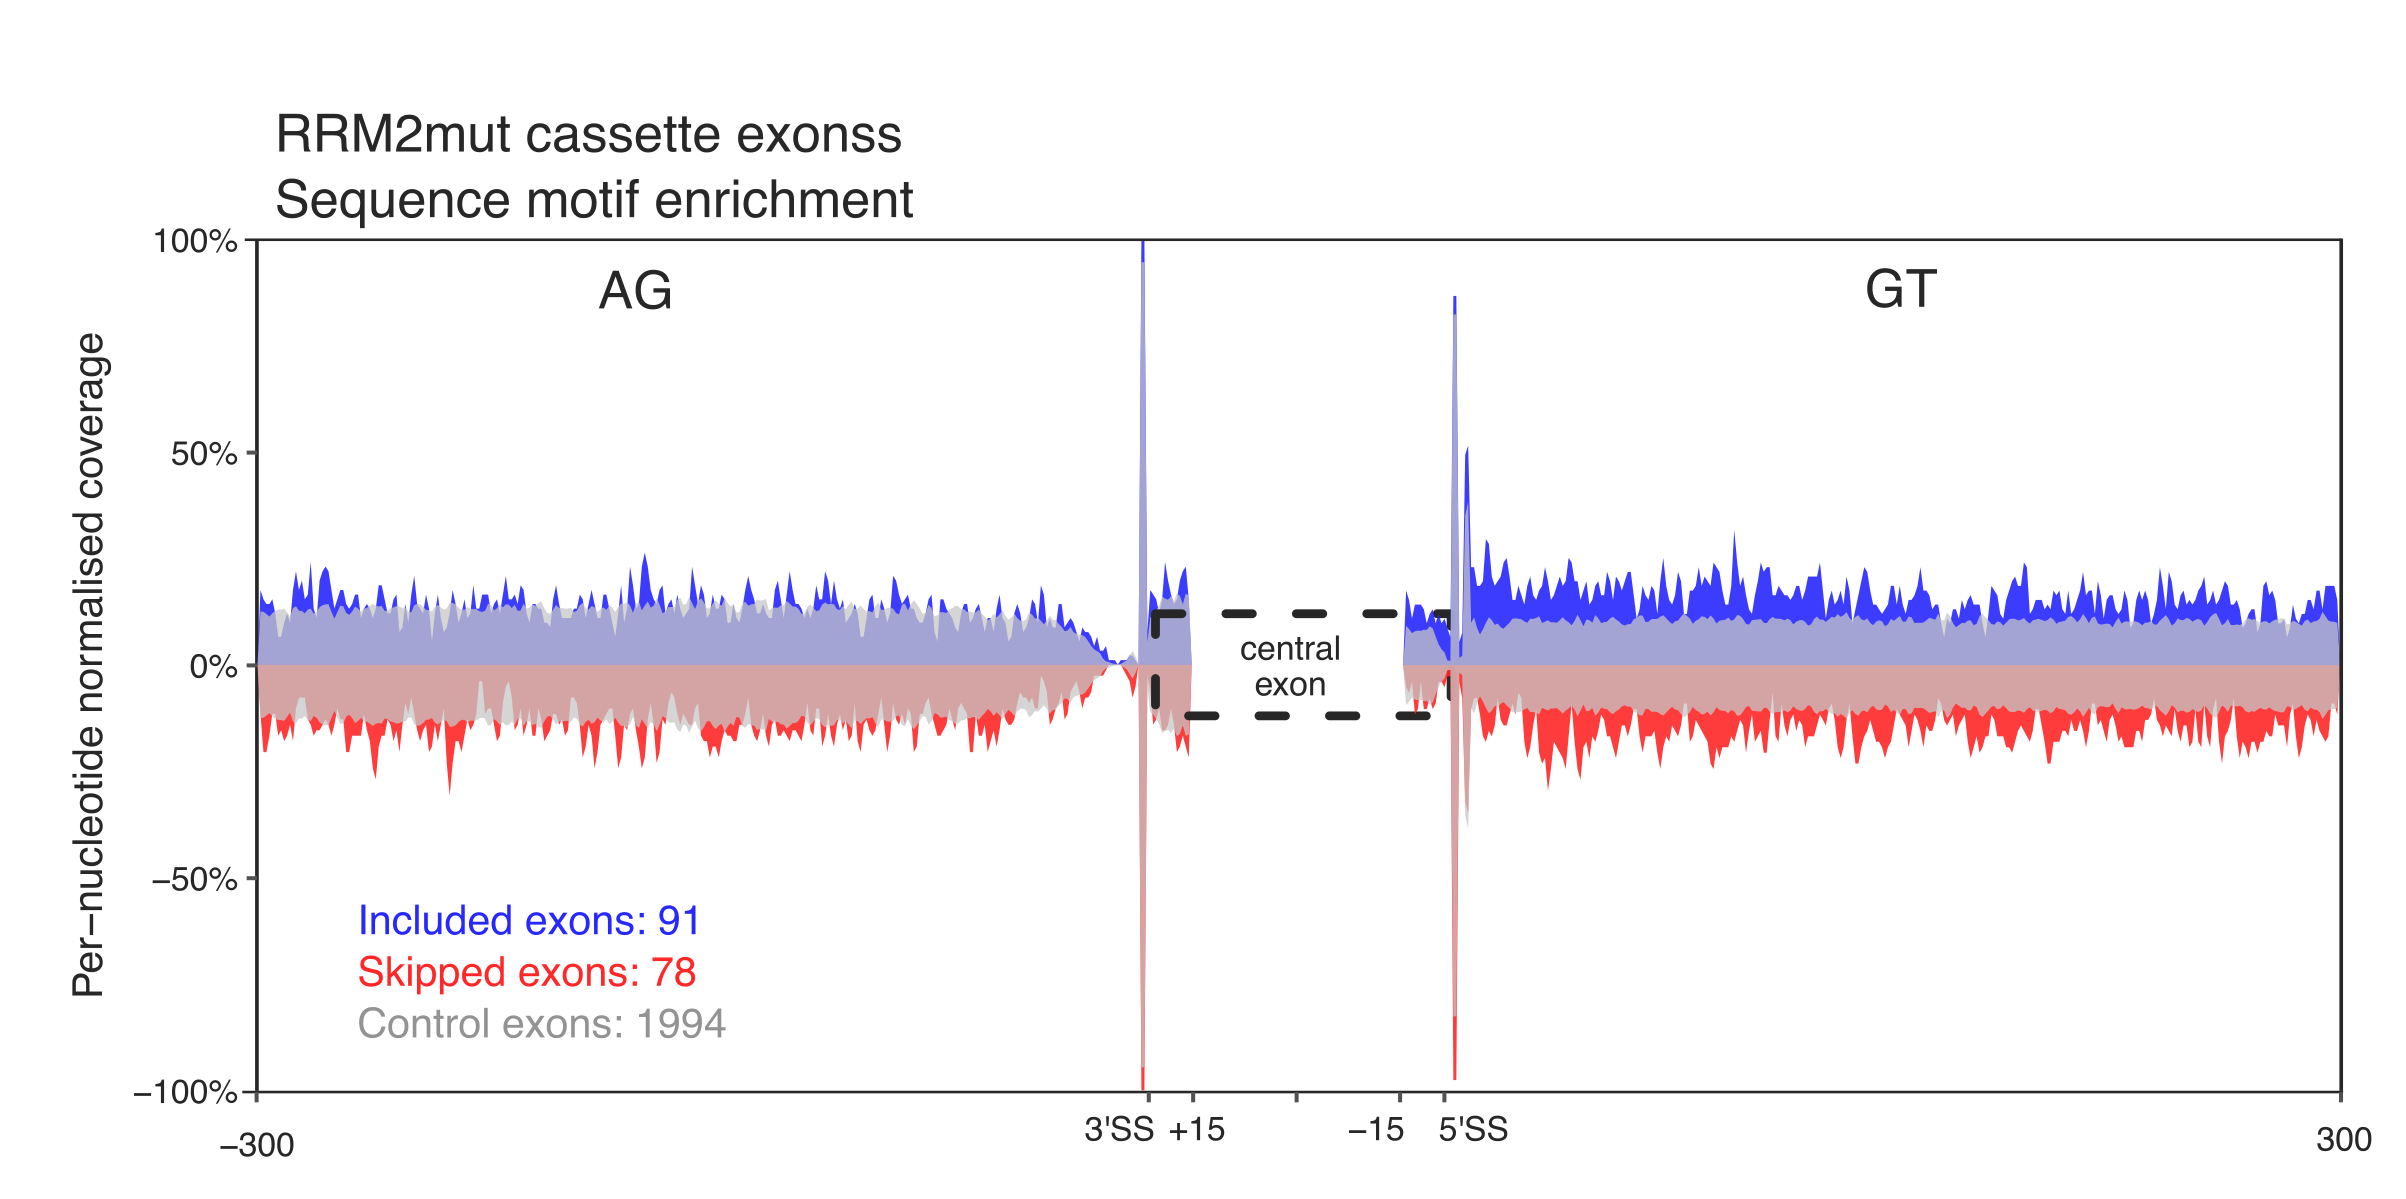
\includegraphics[width=14cm]{Figures/05_tdp_mice/RNAmap_motif_AG_GT_RRM2mut.png}
	\caption{\textbf{RNA maps of AG and GT dinucleotides are invariant at the 5' and 3' splice sites}}
	RNAmaps constructed from differentially included (blue) and skipped (red) cassette exons from RRM2mut.
	
	\label{fig:RNAmap_splicing}
\end{figure}


% Skiptic permutation

\begin{table}[!htbp] \centering 
	
	\footnotesize
	\caption{Results of permuting sample order and repeating splicing analysis. Exons refers to the number of differentially spliced exons found at FDR 5\%, cryptics are those that satisfy the cryptic exon critera and skiptics are those that satisfy the skiptic exon criteria (see chapter). Groups in bold are the correct sample ordering. Note that definitions of skiptic and cryptic depend on which condition is the reference, which accounts for the different numbers between the two correct orderings. } 
	\label{append:permutations} 
	\begin{tabular}{@{\extracolsep{5pt}} cccc} 
		\\[-1.8ex]\hline 
		\hline \\[-1.8ex] 
		groups & exons & cryptic & skiptic \\ 
		\hline \\[-1.8ex] 
		\textbf{M323K\_WT\_1+M323K\_WT\_2+M323K\_WT\_3+M323K\_WT\_4} & 920 & 2 & 47 \\ 
		\textbf{M323K\_HOM\_1+M323K\_HOM\_2+M323K\_HOM\_3+M323K\_HOM\_4} & 920 & 4 & 9 \\ 
		M323K\_HOM\_2+M323K\_HOM\_3+M323K\_HOM\_4+M323K\_WT\_3 & 38 & 0 & 0 \\ 
		M323K\_HOM\_1+M323K\_WT\_1+M323K\_WT\_2+M323K\_WT\_4 & 38 & 0 & 0 \\ 
		M323K\_HOM\_1+M323K\_HOM\_2+M323K\_HOM\_4+M323K\_WT\_4 & 25 & 0 & 1 \\ 
		M323K\_HOM\_3+M323K\_WT\_1+M323K\_WT\_2+M323K\_WT\_3 & 25 & 0 & 0 \\ 
		M323K\_HOM\_1+M323K\_HOM\_3+M323K\_HOM\_4+M323K\_WT\_4 & 25 & 0 & 2 \\ 
		M323K\_HOM\_2+M323K\_WT\_1+M323K\_WT\_2+M323K\_WT\_3 & 25 & 1 & 0 \\ 
		M323K\_HOM\_1+M323K\_HOM\_2+M323K\_HOM\_3+M323K\_WT\_1 & 24 & 0 & 0 \\ 
		M323K\_HOM\_4+M323K\_WT\_2+M323K\_WT\_3+M323K\_WT\_4 & 24 & 0 & 0 \\ 
		M323K\_HOM\_2+M323K\_WT\_1+M323K\_WT\_2+M323K\_WT\_4 & 24 & 1 & 0 \\ 
		M323K\_HOM\_1+M323K\_HOM\_3+M323K\_HOM\_4+M323K\_WT\_3 & 24 & 0 & 0 \\ 
		M323K\_HOM\_1+M323K\_WT\_1+M323K\_WT\_2+M323K\_WT\_3 & 19 & 0 & 0 \\ 
		M323K\_HOM\_2+M323K\_HOM\_3+M323K\_HOM\_4+M323K\_WT\_4 & 19 & 1 & 0 \\ 
		M323K\_HOM\_1+M323K\_HOM\_2+M323K\_HOM\_4+M323K\_WT\_2 & 17 & 0 & 0 \\ 
		M323K\_HOM\_1+M323K\_HOM\_2+M323K\_HOM\_3+M323K\_WT\_3 & 15 & 0 & 0 \\ 
		M323K\_HOM\_4+M323K\_WT\_1+M323K\_WT\_2+M323K\_WT\_4 & 15 & 0 & 0 \\ 
		M323K\_HOM\_2+M323K\_HOM\_3+M323K\_HOM\_4+M323K\_WT\_1 & 12 & 0 & 0 \\ 
		M323K\_HOM\_1+M323K\_HOM\_2+M323K\_HOM\_3+M323K\_WT\_4 & 7 & 0 & 0 \\ 
		M323K\_HOM\_1+M323K\_HOM\_3+M323K\_HOM\_4+M323K\_WT\_2 & 7 & 0 & 0 \\ 
		M323K\_HOM\_4+M323K\_WT\_1+M323K\_WT\_2+M323K\_WT\_3 & 7 & 0 & 0 \\ 
		M323K\_HOM\_3+M323K\_WT\_2+M323K\_WT\_3+M323K\_WT\_4 & 7 & 0 & 0 \\ 
		M323K\_HOM\_1+M323K\_HOM\_3+M323K\_HOM\_4+M323K\_WT\_1 & 5 & 0 & 0 \\ 
		M323K\_HOM\_2+M323K\_WT\_2+M323K\_WT\_3+M323K\_WT\_4 & 5 & 0 & 0 \\ 
		M323K\_HOM\_3+M323K\_WT\_1+M323K\_WT\_2+M323K\_WT\_4 & 2 & 0 & 0 \\ 
		M323K\_HOM\_1+M323K\_HOM\_2+M323K\_HOM\_3+M323K\_WT\_2 & 1 & 0 & 0 \\ 
		M323K\_HOM\_4+M323K\_WT\_1+M323K\_WT\_3+M323K\_WT\_4 & 1 & 0 & 0 \\ 
		M323K\_HOM\_3+M323K\_HOM\_4+M323K\_WT\_3+M323K\_WT\_4 & 51 & 0 & 0 \\ 
		M323K\_HOM\_1+M323K\_HOM\_4+M323K\_WT\_1+M323K\_WT\_4 & 11 & 0 & 0 \\ 
		M323K\_HOM\_2+M323K\_HOM\_3+M323K\_WT\_2+M323K\_WT\_3 & 11 & 0 & 0 \\ 
		M323K\_HOM\_1+M323K\_HOM\_2+M323K\_WT\_1+M323K\_WT\_3 & 11 & 1 & 0 \\ 
		M323K\_HOM\_3+M323K\_HOM\_4+M323K\_WT\_2+M323K\_WT\_4 & 11 & 0 & 0 \\ 
		M323K\_HOM\_2+M323K\_HOM\_4+M323K\_WT\_3+M323K\_WT\_4 & 11 & 0 & 0 \\ 
		M323K\_HOM\_2+M323K\_HOM\_3+M323K\_WT\_1+M323K\_WT\_3 & 9 & 0 & 0 \\ 
		M323K\_HOM\_1+M323K\_HOM\_4+M323K\_WT\_2+M323K\_WT\_4 & 9 & 0 & 0 \\ 
		M323K\_HOM\_1+M323K\_HOM\_2+M323K\_WT\_3+M323K\_WT\_4 & 9 & 0 & 0 \\ 
		M323K\_HOM\_3+M323K\_HOM\_4+M323K\_WT\_1+M323K\_WT\_2 & 9 & 0 & 0 \\ 
		M323K\_HOM\_2+M323K\_HOM\_3+M323K\_WT\_1+M323K\_WT\_4 & 9 & 0 & 0 \\ 
		M323K\_HOM\_2+M323K\_HOM\_3+M323K\_WT\_3+M323K\_WT\_4 & 7 & 0 & 0 \\ 
		M323K\_HOM\_1+M323K\_HOM\_4+M323K\_WT\_1+M323K\_WT\_2 & 7 & 0 & 0 \\ 
		M323K\_HOM\_3+M323K\_HOM\_4+M323K\_WT\_2+M323K\_WT\_3 & 6 & 0 & 0 \\ 
		M323K\_HOM\_1+M323K\_HOM\_2+M323K\_WT\_1+M323K\_WT\_4 & 6 & 0 & 0 \\ 
		M323K\_HOM\_2+M323K\_HOM\_3+M323K\_WT\_1+M323K\_WT\_2 & 4 & 0 & 0 \\ 
		M323K\_HOM\_1+M323K\_HOM\_4+M323K\_WT\_3+M323K\_WT\_4 & 4 & 0 & 0 \\ 
		M323K\_HOM\_1+M323K\_HOM\_2+M323K\_WT\_2+M323K\_WT\_4 & 4 & 0 & 1 \\ 
		M323K\_HOM\_2+M323K\_HOM\_3+M323K\_WT\_2+M323K\_WT\_4 & 3 & 0 & 0 \\ 
		M323K\_HOM\_3+M323K\_HOM\_4+M323K\_WT\_1+M323K\_WT\_4 & 21 & 0 & 1 \\ 
		M323K\_HOM\_2+M323K\_HOM\_4+M323K\_WT\_2+M323K\_WT\_4 & 18 & 0 & 0 \\ 
		M323K\_HOM\_1+M323K\_HOM\_3+M323K\_WT\_3+M323K\_WT\_4 & 16 & 0 & 0 \\ 
		M323K\_HOM\_2+M323K\_HOM\_4+M323K\_WT\_1+M323K\_WT\_2 & 16 & 0 & 0 \\ 
		M323K\_HOM\_1+M323K\_HOM\_3+M323K\_WT\_2+M323K\_WT\_4 & 14 & 0 & 1 \\ 
		M323K\_HOM\_2+M323K\_HOM\_4+M323K\_WT\_1+M323K\_WT\_4 & 2 & 0 & 0 \\ 
		\hline \\[-1.8ex] 
	\end{tabular} 
\end{table} 

% fibroblast sample info
\begin{table}[!htbp] \centering 
	\caption{Information on human fibroblast lines used. B,	bulbar;	UL, upper limb;	LL,	lower limb} 
	\label{append:fibros} 
	\begin{tabular}{@{\extracolsep{5pt}} ccccccc} 
		\\[-1.8ex]\hline 
		\hline \\[-1.8ex] 
		Fibroblast line & Mutation & Diagnosis & Age at onset & Site of onset & Gender & Age at biopsy \\ 
		\hline \\[-1.8ex] 
		TARDBP 1 & G298S & ALS & 62 & LL & M & 64 \\ 
		TARDBP 2 & A382T & ALS & 59 & UL & F & 62 \\ 
		TARDBP 3 & A382T & ALS & 25 & LL & F & 31 \\ 
		TARDBP 4 & A382T & ALS & 67 & B & M & 69 \\ 
		CTRL 1 & . & Healthy & . & . & F & 67 \\ 
		CTRL 2 & . & Healthy & . & . & M & 64 \\ 
		CTRL 3 & . & Healthy & . & . & M & 67 \\ 
		CTRL 4 & . & Healthy & . & . & F & 69 \\ 
		\hline \\[-1.8ex] 
	\end{tabular} 
\end{table} 


% skiptics list
\begin{table}[!htbp] \centering 
	\caption{List of skiptic exons found in LCDmut adult brain} 
	\label{append:skiptics} 
	\footnotesize
\begin{tabular}{@{\extracolsep{5pt}} ccccccccc} 
	
	\\[-1.8ex]\hline 
	\hline \\[-1.8ex] 
	chr & start & end & Gene & PSI\textsubscript{WT} & PSI\textsubscript{LCDmut} & $\Delta$PSI & fold change & \textit{q} \\ 
	\hline \\[-1.8ex] 
	chr2 & 144502918 &144503031 & \textit{Dzank1} & 0.9795 & 0.8160 & $-0.164$ & 8.9942 & 1.57E$-45$ \\ 
	chr7 & 56157784 & 56163742 & \textit{Herc2} & 0.9983 & 0.7828 & $-0.216$ & 128.6068 & 4.71E$-42$\\ 
	chr5 & 29597184 & 29600641 & \textit{Ube3c} & 0.9894 & 0.7449 & $-0.244$ & 24.1694 & 1.62E$-40$\\ 
	chr10 & 78284350 & 78287847 & \textit{Agpat3} & 0.9964 & 0.9011 & $-0.095$ & 27.1469 & 1.73E$-32$ \\ 
	chr5 & 36947237 & 36952351 & \textit{Ppp2r2c} & 0.9993 & 0.9359 & $-0.063$ & 94.4229 & 1.71E$-26$\\ 
	chr1 & 118304691  &118304770& \textit{Tsn} & 0.9978 & 0.9012 & $-0.096$ & 44.3227 & 7.36E$-23$ \\ 
	chr6 & 113492124  & 113492258 & \textit{Creld1} & 1.0000 & 0.8747 & $-0.125$ & \textgreater 150 & 1.05E$-22$ \\ 
	chr12 & 50365712 & 50383400 & \textit{Prkd1} & 0.9804 & 0.4517 & $-0.529$ & 28.0231 & 4.99E$-18$\\ 
	chr4 & 19618357 & 19621928 & \textit{Wwp1} & 0.9984 & 0.9111 & $-0.087$ & 56.7242 & 2.13E$-17$ \\ 
	chr4 & 58817550 & 58820128 & \textit{AI314180} & 0.9981 & 0.9037 & $-0.094$ & 51.0528 & 1.49E$-16$\\ 
	chr19 & 38265097 & 38283970 & \textit{Lgi1} & 0.9847 & 0.8165 & $-0.168$ & 11.9947 & 1.09E$-14$\\ 
	chr11 & 101317623  &101317727 & \textit{Psme3} & 0.9632 & 0.8737 & $-0.090$ & 3.4328 & 2.61E$-14$\\ 
	chr7 & 56184707 & 56185835 & \textit{Herc2} & 0.9881 & 0.8836 & $-0.104$ & 9.8083 & 1.25E$-13$\\ 
	chr5 & 108642696  & 108642779& \textit{Tmem175} & 0.9514 & 0.7273 & $-0.224$ & 5.6106 & 6.73E$-12$\\ 
	chr11 & 45852192 & 45884332 & \textit{Clint1} & 0.9962 & 0.8842 & $-0.112$ & 30.5766 & 1.85E$-10$ \\ 
	chr10 & 7710647 & 7712501 & \textit{Lats1} & 0.9959 & 0.9221 & $-0.074$ & 19.0151 & 5.18E$-9$\\ 
	chr11 & 97242047 & 97244428 & \textit{Npepps} & 0.9954 & 0.9425 & $-0.053$ & 12.6145 & 5.99E$-9$\\ 
	chr11 & 100440040 & 100440086 & \textit{Nt5c3b} & 0.9709 & 0.8464 & $-0.125$ & 5.2820 & 1.21E$-7$\\ 
	chr17 & 22428565 & 22446797 & \textit{Zfp946} & 0.9530 & 0.6858 & $-0.267$ & 6.6817 & 5.79E$-7$ \\ 
	chr2 & 130713397  & 130713503& \textit{4930402H24Rik} & 0.9908 & 0.9386 & $-0.052$ & 6.6376 & 7.23E$-7$ \\ 
	chr13 & 13638376 & 13641067 & \textit{Lyst} & 0.9909 & 0.8287 & $-0.162$ & 18.8410 & 8.97E$-7$\\ 
	chr6 & 30439865 & 30444427 & \textit{Klhdc10} & 0.9721 & 0.8957 & $-0.076$ & 3.7346 & 1.97E$-6$\\ 
	chr19 & 40340146 & 40344356 & \textit{Sorbs1} & 0.9877 & 0.8305 & $-0.157$ & 13.7569 & 2.29E$-6$\\ 
	chr5 & 8143132 & 8145553 & \textit{Adam22} & 0.9881 & 0.8977 & $-0.090$ & 8.5959 & 4.96E$-6$ \\ 
	chr14 & 18630431 & 18888266 & \textit{Ube2e2} & 0.9542 & 0.8915 & $-0.063$ & 2.3700 & 8.43E$-6$\\ 
	chr7 & 126153199 & 26153279 & \textit{Xpo6} & 0.9657 & 0.8754 & $-0.090$ & 3.6328 & 2.37E$-5$ \\ 
	chr8 &  105194475 & 105194591 & \textit{Cbfb} & 0.9736 & 0.8752 & $-0.098$ & 4.7209 & 4.06E$-5$ \\ 
	chr6 & 8216470 & 8224555 & \textit{Mios} & 0.9674 & 0.9026 & $-0.065$ & 2.9852 & 0.000146 \\ 
	chr5 & 9131308 & 9136066 & \textit{Dmtf1} & 0.9683 & 0.8230 & $-0.145$ & 5.5848 & 0.00015 \\ 
	chr16 & 17845135 & 17856752 & \textit{Dgcr2} & 0.9879 & 0.9334 & $-0.054$ & 5.4902 & 0.000182 \\ 
	chr16 & 94408716 & 94410833 & \textit{Ttc3} & 0.9925 & 0.8888 & $-0.104$ & 14.8993 & 0.000244 \\ 
	chr4 & 59592318 & 59594396 & \textit{Hsdl2} & 0.9801 & 0.9262 & $-0.054$ & 3.7039 & 0.000247 \\ 
	chr2 & 69741693 & 69746028 & \textit{Ppig} & 0.9725 & 0.9024 & $-0.070$ & 3.5489 & 0.00025 \\ 
	chr7 & 141526432  & 141526493 & \textit{Chid1} & 0.9876 & 0.9272 & $-0.060$ & 5.8899 & 0.000367 \\ 
	chr11 & 79242156 & 79244463 & \textit{Wsb1} & 0.9588 & 0.8991 & $-0.060$ & 2.4516 & 0.000532 \\ 
	chr1 & 119706155  & 119706313 & \textit{Ptpn4} & 0.9793 & 0.8764 & $-0.103$ & 5.9574 & 0.000597 \\ 
	chr10 & 83737933 & 83758134 & \textit{1500009L16Rik} & 0.9938 & 0.8995 & $-0.094$ & 16.2830 & 0.000837 \\ 
	chr8 & 75051657 & 75052150 & \textit{Tom1} & 0.9947 & 0.9301 & $-0.065$ & 13.2732 & 0.000883 \\ 
	chr11 & 58848702 & 58856061 & \textit{Gm12258} & 1.0000 & 0.8671 & $-0.133$ & \textgreater 150 & 0.000917 \\ 
	chr9 & 55858525 & 55859748 & \textit{Scaper} & 1.0000 & 0.8226 & $-0.177$ & \textgreater 150 & 0.001059 \\ 
	chr17 & 34905456 & 34905910 & \textit{Ehmt2} & 0.9718 & 0.8790 & $-0.093$ & 4.2930 & 0.001613 \\ 
	chr14 & 56957103 & 56959715 & \textit{Zmym2} & 0.9958 & 0.9412 & $-0.055$ & 14.0286 & 0.001684 \\ 
	chr5 & 110396045 & 110396074& \textit{Fbrsl1} & 0.9800 & 0.7715 & $-0.208$ & 11.4248 & 0.002646 \\ 
	chr5 & 3610288 & 3615075 & \textit{Pex1} & 1.0000 & 0.8614 & $-0.139$ & \textgreater 150 & 0.004794 \\ 
	chr9 & 54477528 & 54501351 & \textit{Dmxl2} & 0.9831 & 0.9073 & $-0.076$ & 5.4917 & 0.005274 \\ 
	chr17 & 75540191 & 75544748 & \textit{Fam98a} & 0.9778 & 0.8999 & $-0.078$ & 4.5140 & 0.0057 \\ 
	chr11 & 96773222 & 96776968 & \textit{Snx11} & 0.9873 & 0.9256 & $-0.062$ & 5.8572 & 0.008094 \\ 
	\hline \\[-1.8ex] 
	\end{tabular} 
	\end{table} 
	
\clearpage

\section*{Appendices to \autoref{chapter:fus_meta} }

%Scatter plots explainign the strict and relaxed overlaps
\begin{figure}[h]
	\centering
	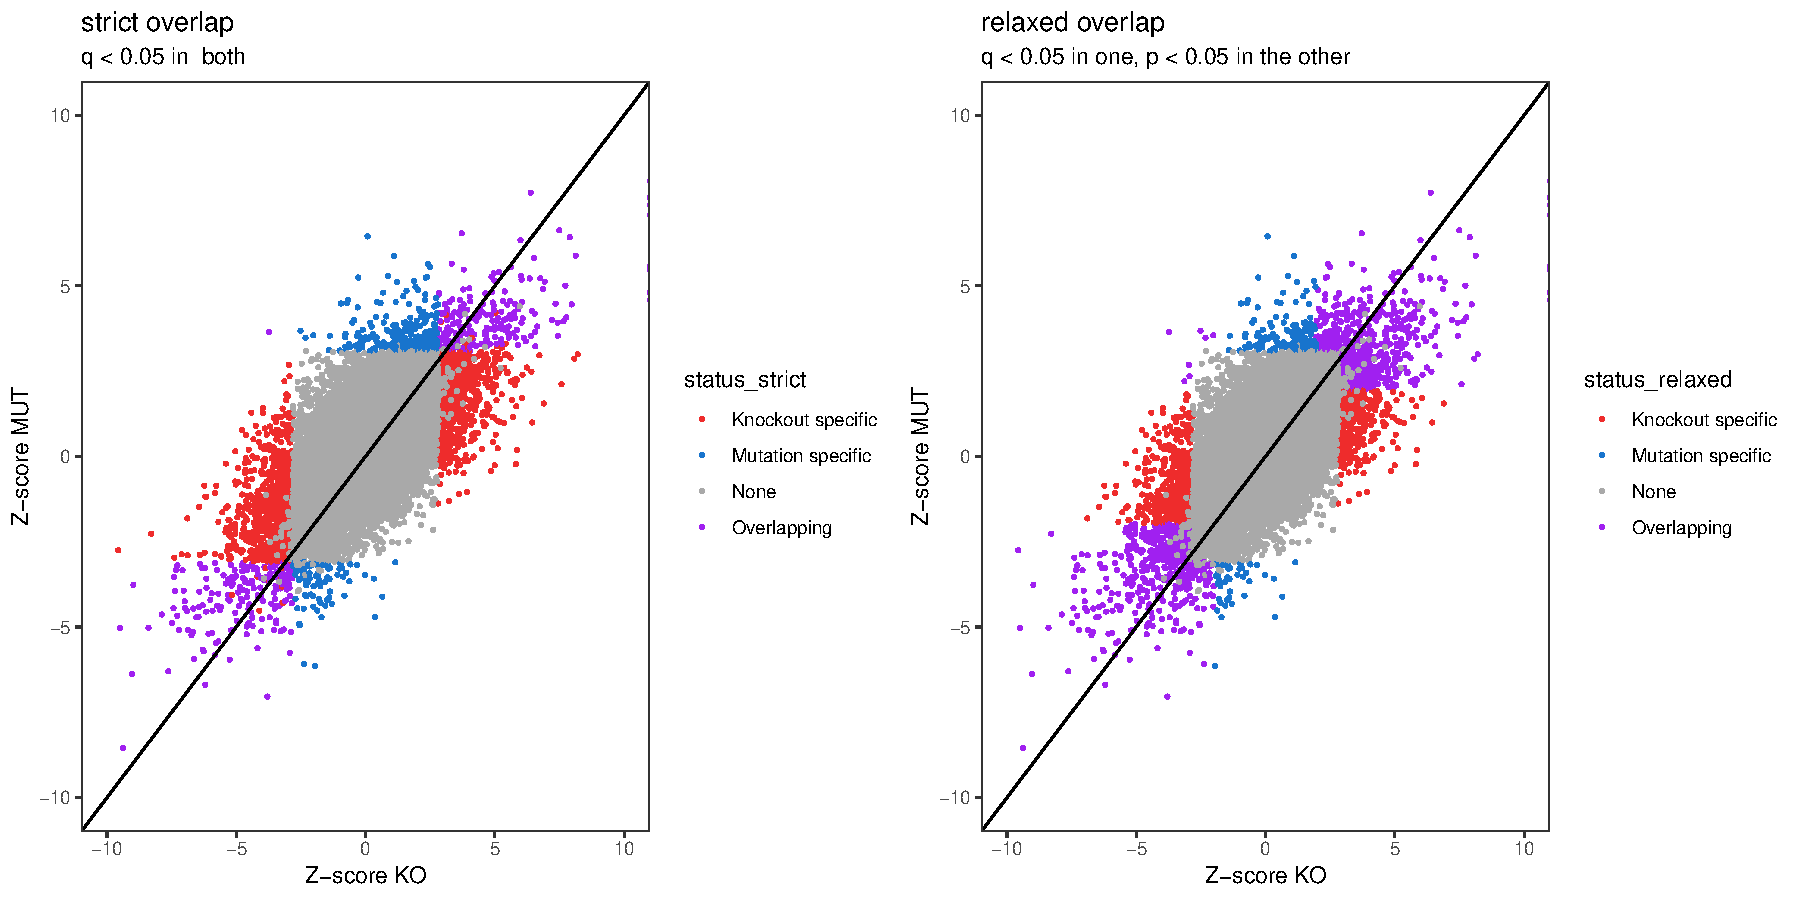
\includegraphics[width=\textwidth]{Figures/06_fus_meta/overlap_type_z_score_plot.pdf}
	\caption{\textbf{Strict and relaxed overlaps of differential expressed genes between FUS KO and FUS MUT joint models.}}
			Each gene plotted as a signed Z-score comparisons constructed from the raw p-value and the sign of the estimated $log_2$ fold change.

	\label{fig:fus_zscore_overlap}
\end{figure}


%Imputing sex from chrY expression
\begin{figure}
	\centering
	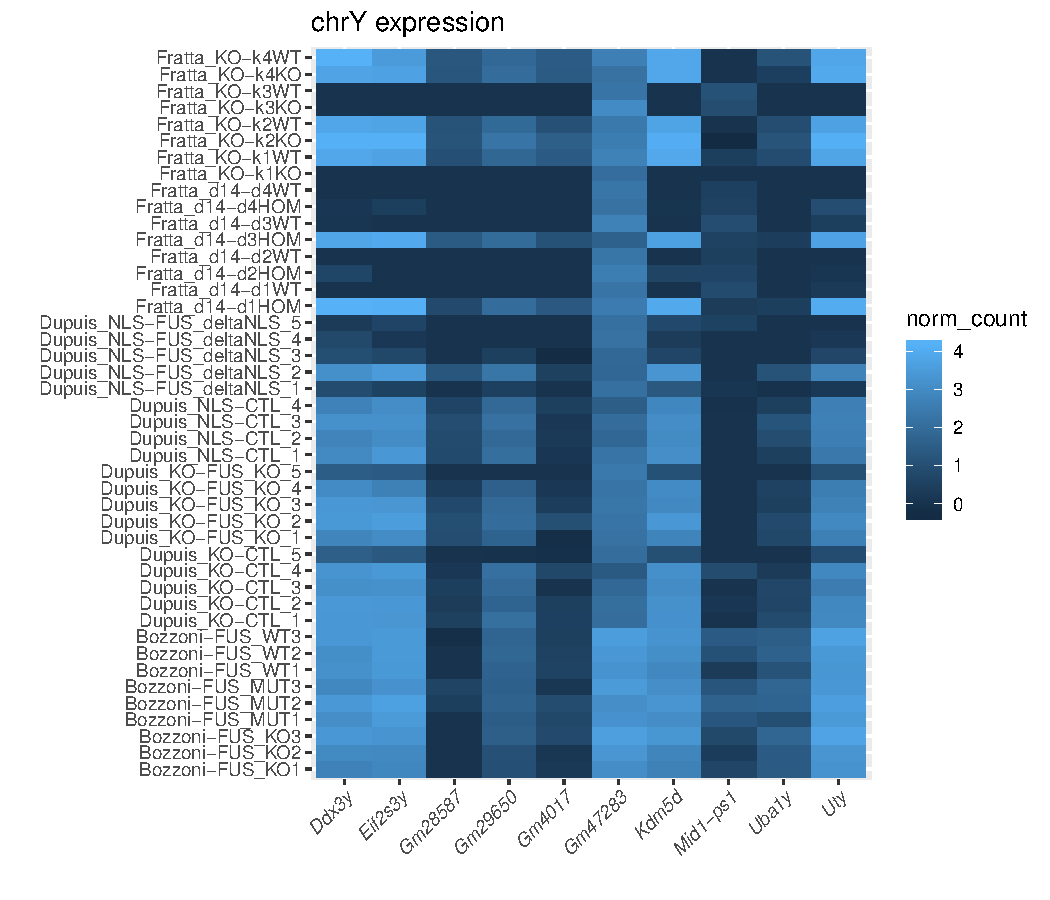
\includegraphics[width=\textwidth]{Figures/06_fus_meta/sex_heatmap.pdf}
	\caption{\textbf{ chrY expression for each sample allows for sex to be imputated } }
	The top 10 most highly expressed mouse Y chromosome genes are plotted for each sample with a library-size normalised read count.
	One gene, Gm47283 shows expression in all samples due to it having a paralogue on the X chromosome. 
	The other 9 genes clearly separate samples in to two groups. 
	All Bozzoni samples appear to be male, whereas Dupuis and Fratta samples are mixed.
	
	
	\label{fig:fus_sex_heatmap}
\end{figure}
%RNA-seq traces of 3 splicing events

\begin{figure}
	\centering
	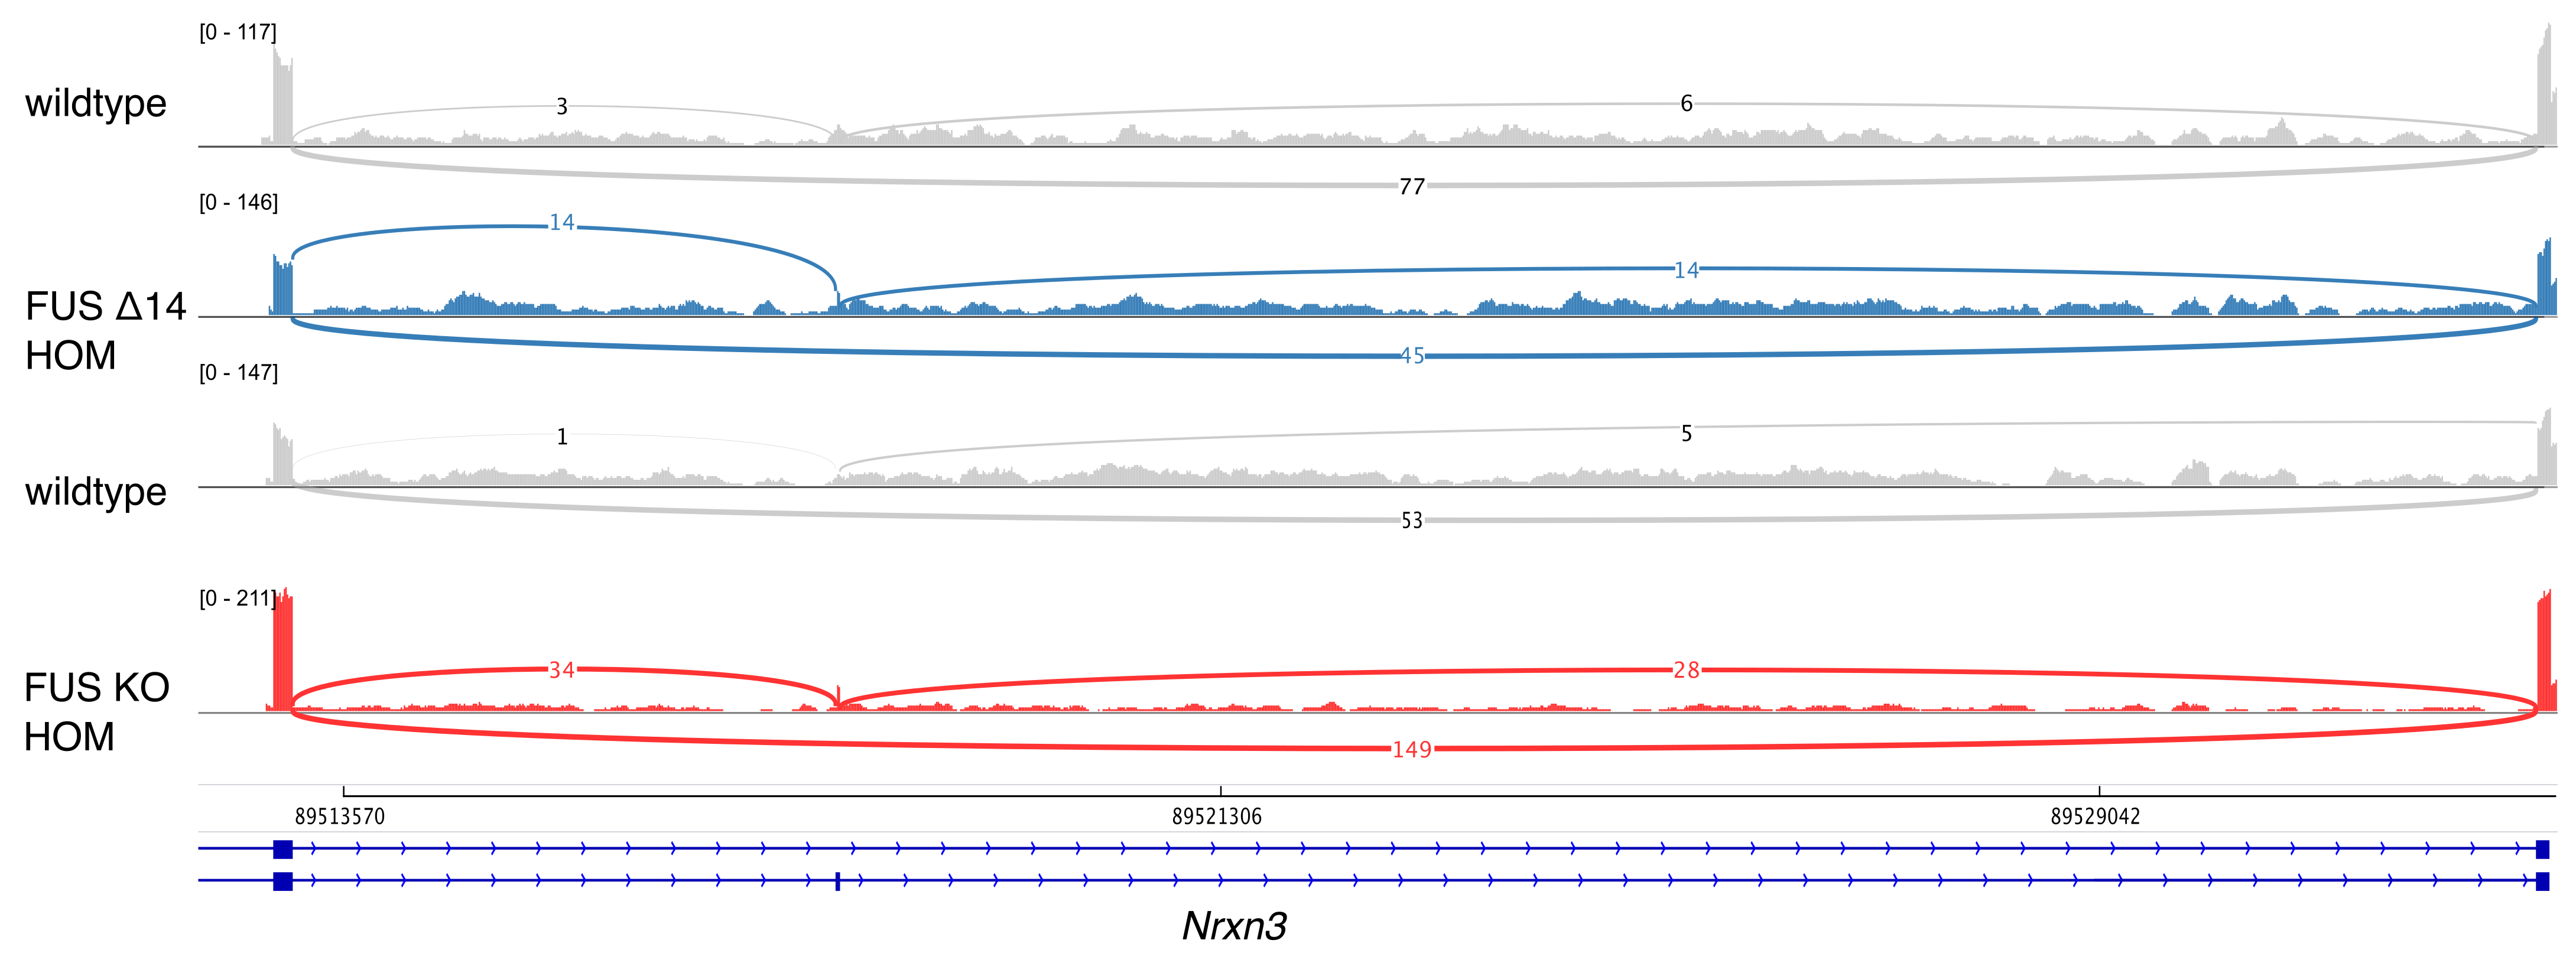
\includegraphics[width=\textwidth]{Figures/06_fus_meta/Nrxn3.png}
	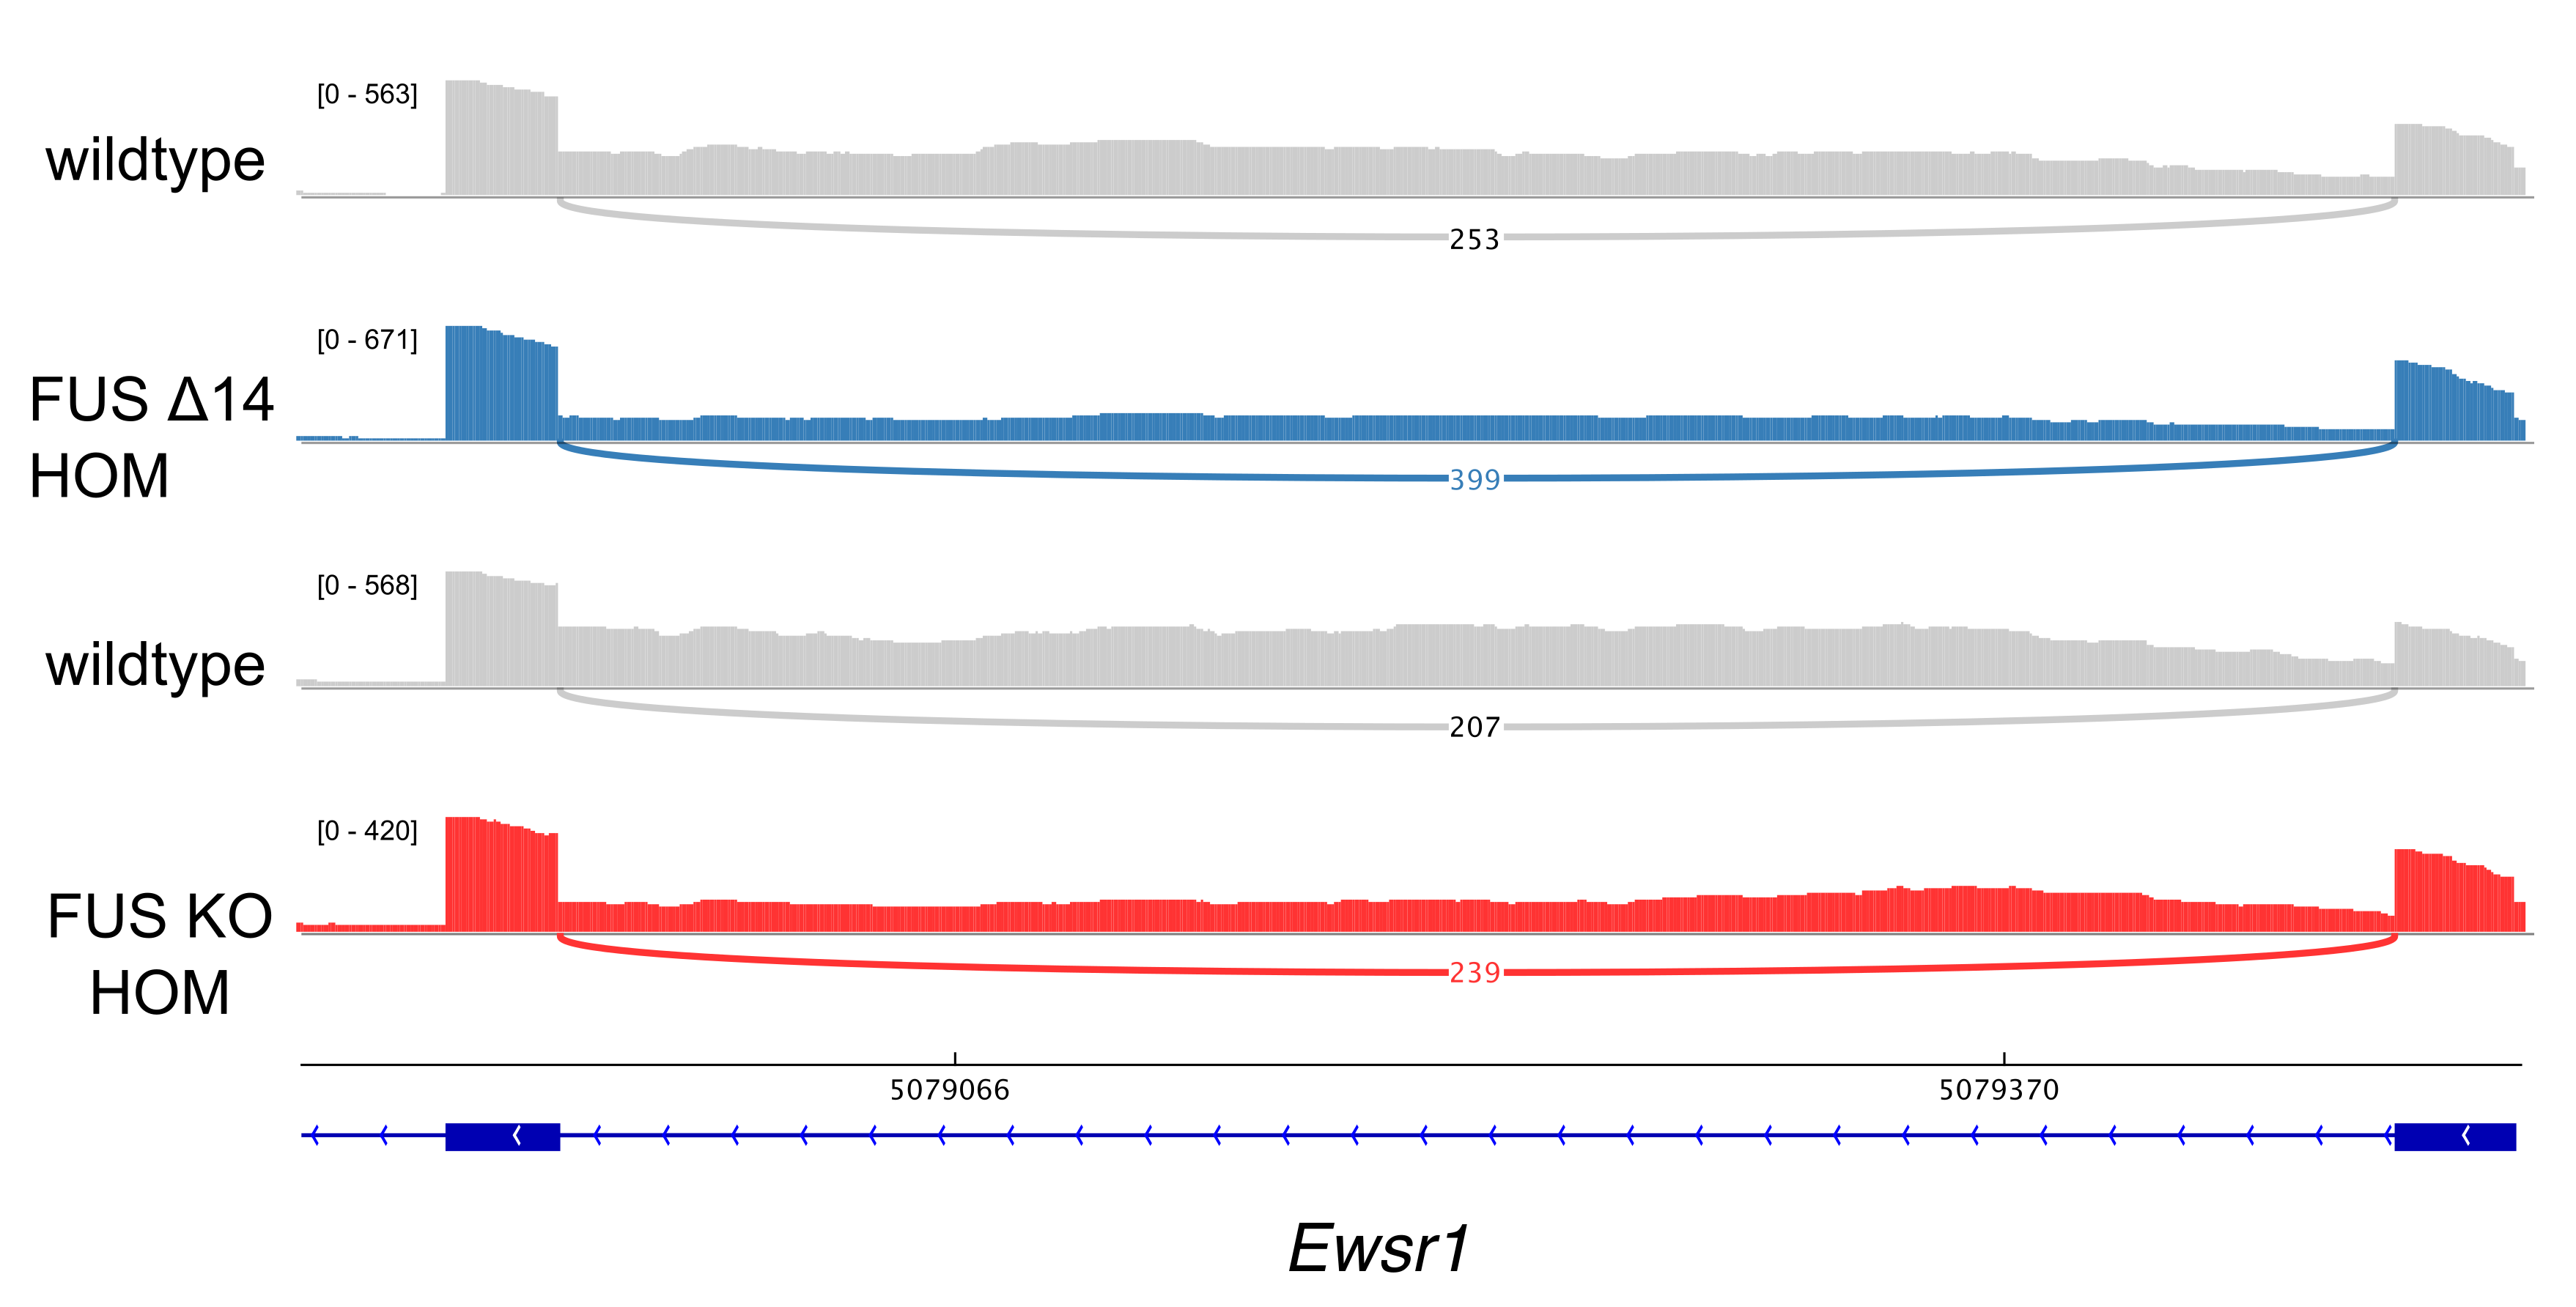
\includegraphics[width=10cm]{Figures/06_fus_meta/Ewsr1.png}
	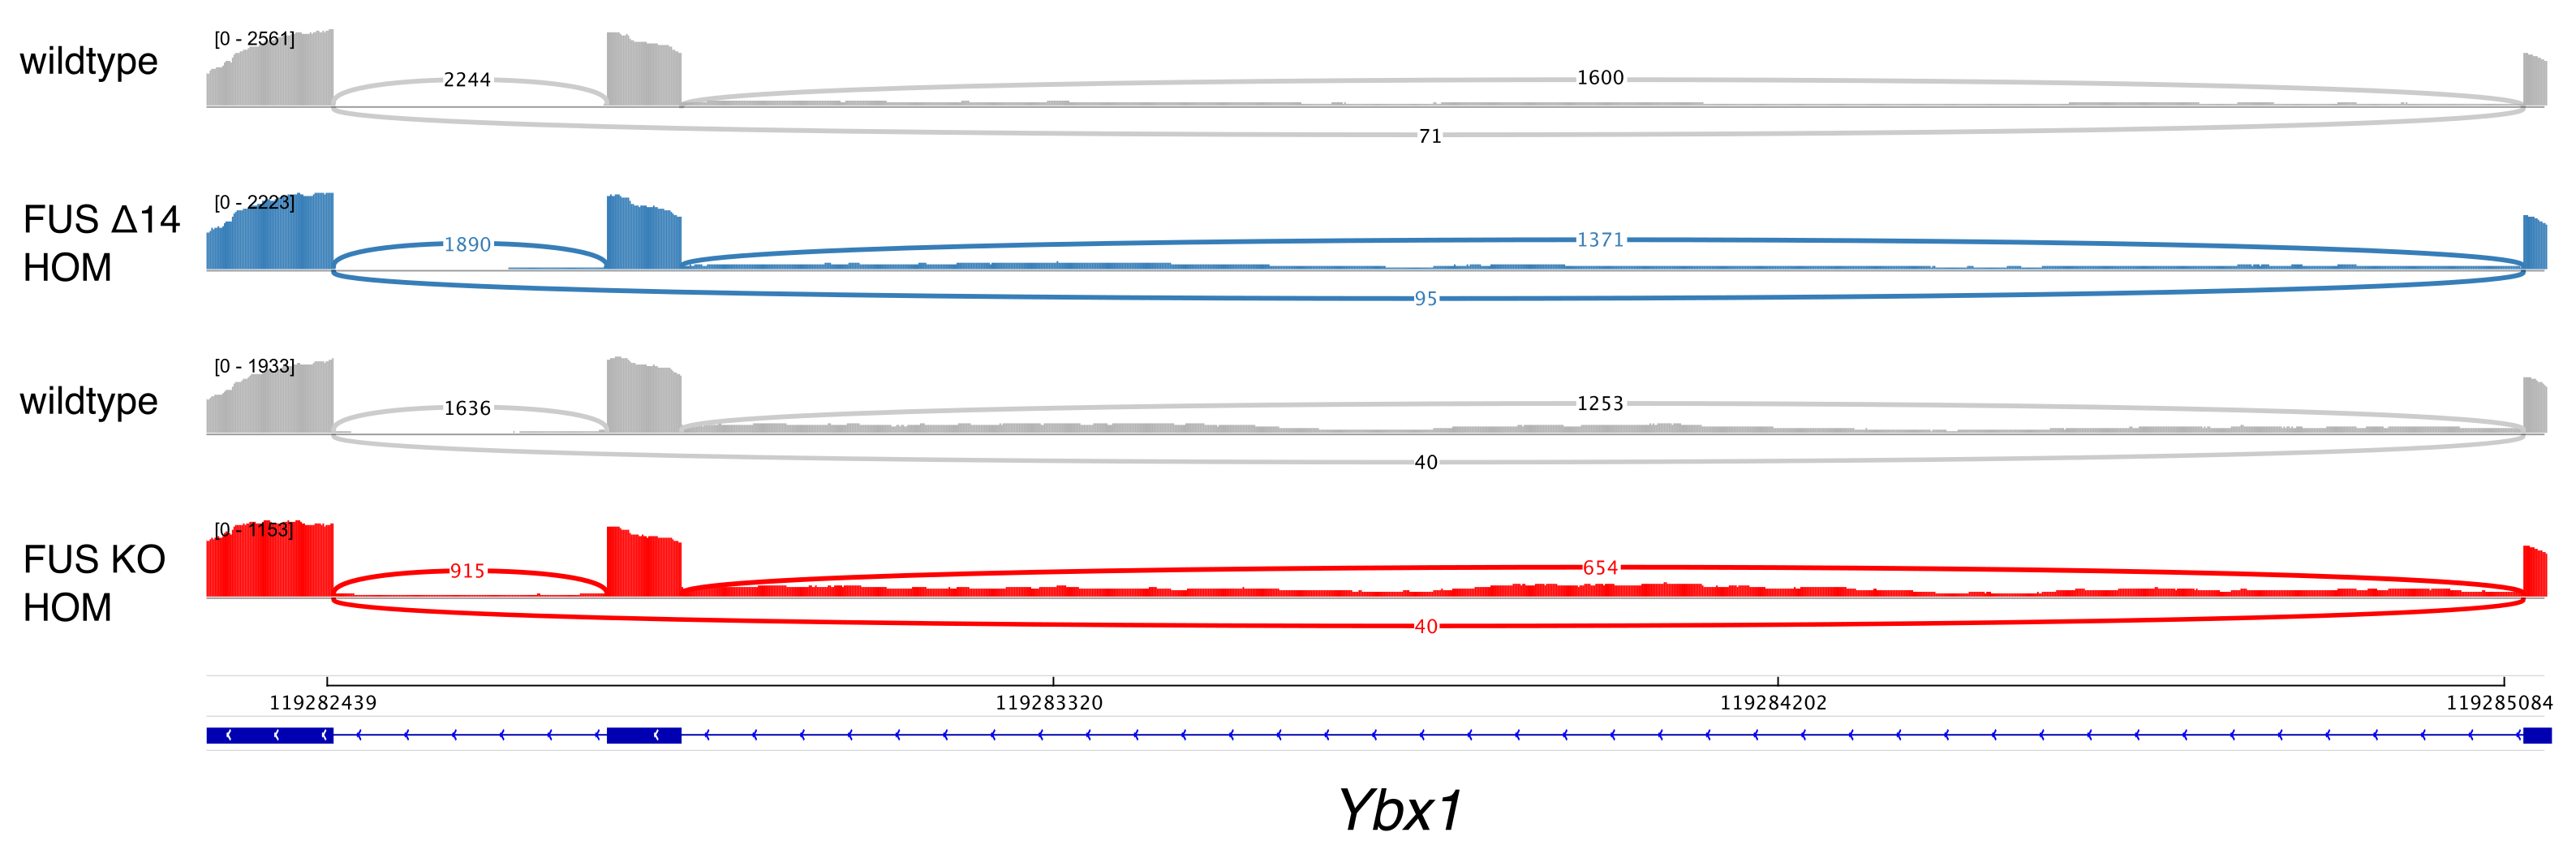
\includegraphics[width=\textwidth]{Figures/06_fus_meta/Ybx1.png}
	\caption{\textbf{RNA-seq traces from three splicing events found in both FUS KO and FUS MUT} }
	Sashimi plots from IGV show read coverage and splice junction counts for a cassette exon in \textit{Nrxn3}, a retained intron in \textit{Ewsr1} and a complex splicing event in \textit{Ybx1}.
	A homozygous FUS$\Delta$14 sample is shown in blue with a littermate control in grey. A homozygous FUS knockout sample is shown in red with its respective littermate control above in grey.
	\label{fig:fus_traces}
\end{figure}




\clearpage

\section*{Publications}

I have attached 4 published papers in which I had a prominent role.


\subsection*{Quantitative analysis of cryptic splicing associated with TDP-43 depletion}

I processed all the RNA-seq data. I designed and performed all analyses with advice and guidance from the other authors. I wrote the manuscript with advice and guidance from the other authors. I am the sole first author.

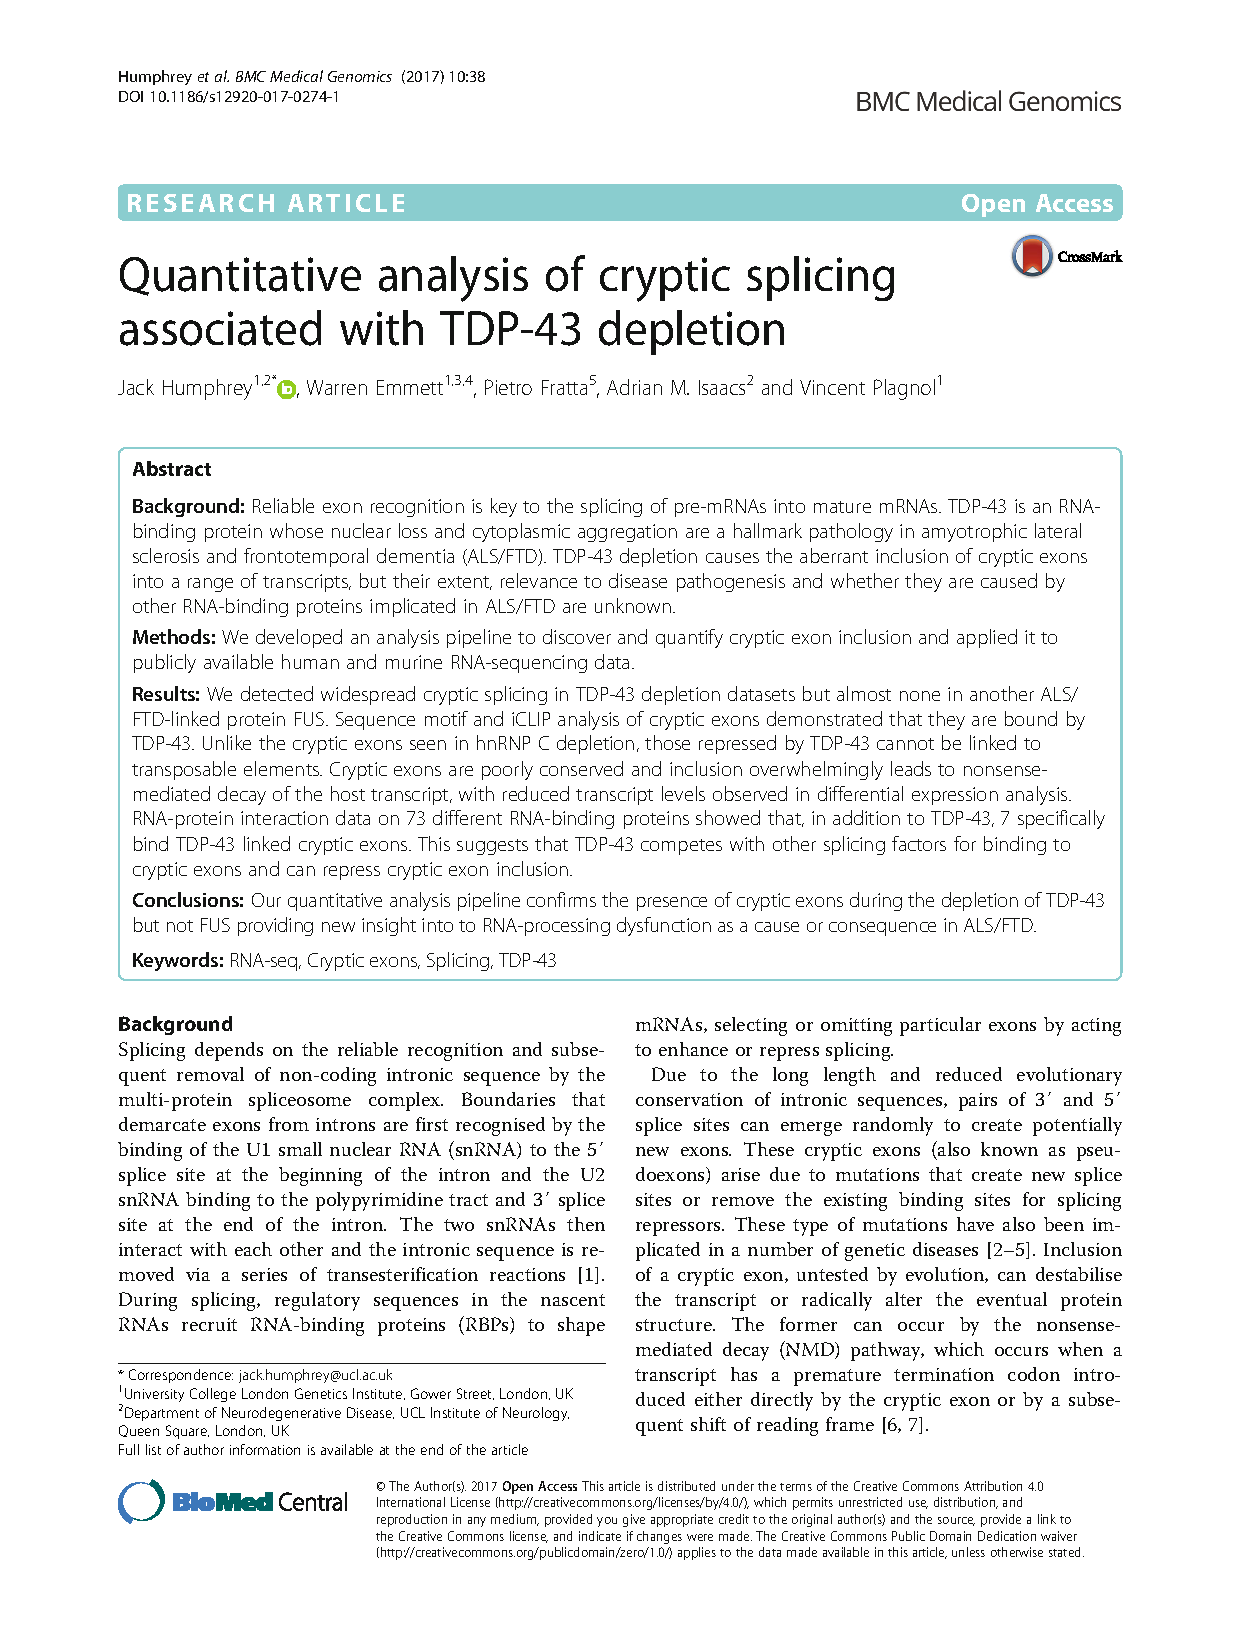
\includepdf[pages=-]{Appendices/Humphrey_Cryptic_Exons.pdf}

\subsection*{Humanized mutant FUS drives progressive motor neuron degeneration without aggregation in FUSDelta14 knockin mice}

I processed all the RNA-seq data. I designed and performed the differential expression and gene ontology analyses presented in Figure 4. I wrote the relevant methods section and assisted Dr Anny Devoy with intepretation of the data from my analyses.

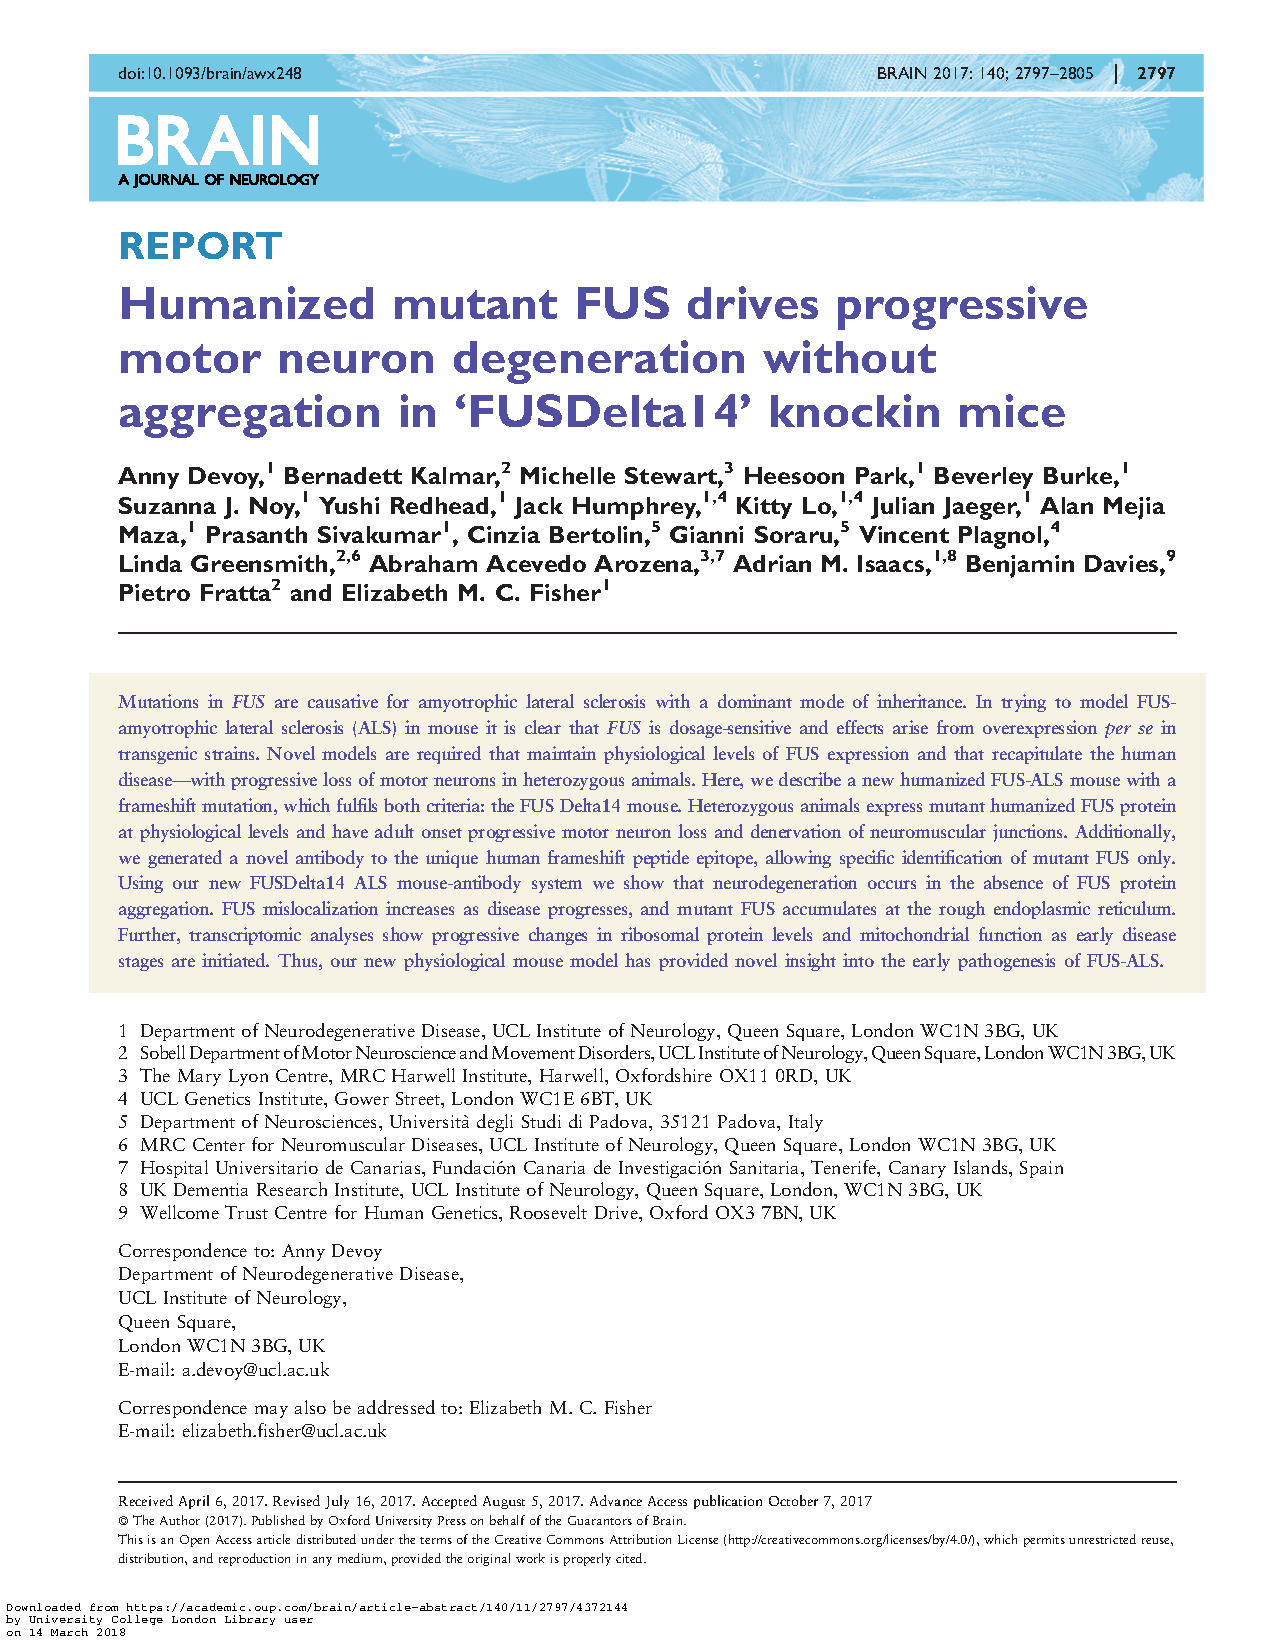
\includepdf[pages=-]{Appendices/Devoy_FUS_mouse.pdf}

\subsection*{Mice with endogenous TDP-43 mutations exhibit gain of splicing function and characteristics of amyotrophic lateral sclerosis}

I processed all the RNA-seq data, assisted by Dr Kitty Lo. Dr Lo and I designed the splicing analyses together and I continued and finished the project after her departure. My work is included in Figures 2 and 5. I contributed to the writing of the manuscript and wrote all the relevant methods section. I received a joint first authorship credit.
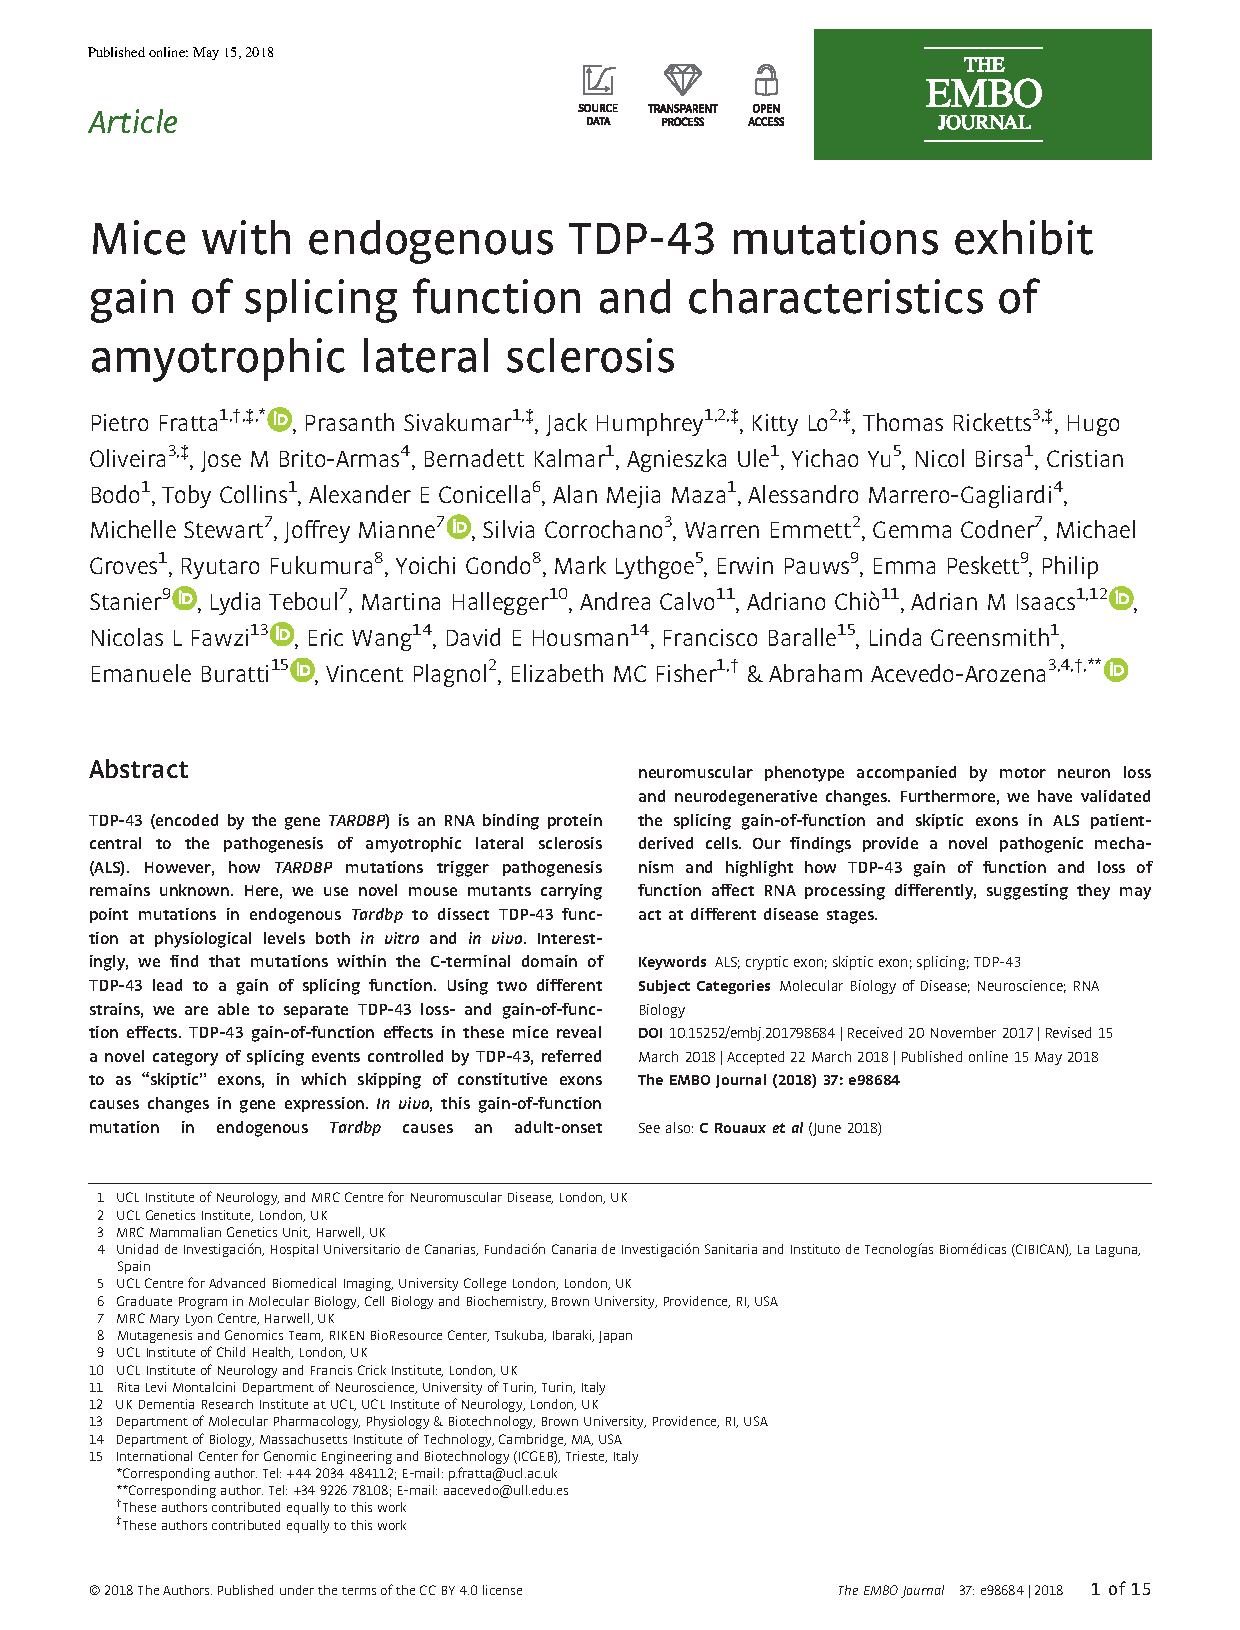
\includepdf[pages=-]{Appendices/Fratta_TDP_mice.pdf}


%\subsection*{Annotation-free quanitification of RNA splicing with Leafcutter}
%
%While on a short fellowship at Stanford University, USA, I was involved in the development of Leafcutter, a software package to run differential splicing analysis on RNA-seq data. I designed and created an interactive web-based application for users to visualise and explore the results of using the tool. A screenshot from the tool is used in Figure 1 of the paper. I am an active maintainer of the Leafcutter Github repository (github.com/davidaknowles/leafcutter)
%\includepdf[pages=1-9]{Appendices/Li_Leafcutter.pdf}

\end{appendices}

% PUBLICATIONS - leave out for github
%\input{Chapters/publications.tex}

\cleardoublepage
\end{document}